\documentclass{article}

% Informations

%Modules 
\usepackage[greek,english,french]{babel}
\usepackage{graphicx}                       % Gestion des images
\usepackage{caption}                        % Gestion des titres
\usepackage{appendix}                       % Gestion de l'annexe
\usepackage[utf8]{inputenc}                 % Encodage du texte
\usepackage{multicol}                       % Gestion des multi-colonnes des tableaux
\usepackage{multirow}
\usepackage{booktabs}                       % Importation des traits horizontaux des tableaux
\usepackage{siunitx}                        % Gestion des unités
\usepackage{mwe,lipsum}                     % Modules de Minimal Working Examples
\usepackage{amsmath,amssymb,amsbsy}         % Ajout d'options dans le mode 'math'
\usepackage{todonotes}                      % Ajout des notes en marge
\usepackage{mathtools}                      % Autres outils pour le mode 'math'
\usepackage[a4paper]{geometry}                       % Options de mise en page
\usepackage{listings}
\usepackage{color,xcolor}
\usepackage{csquotes}
\usepackage{textcomp}
\usepackage{fancyhdr}
\usepackage{lmodern}
\usepackage[T1]{fontenc}
\usepackage{lato}
\usepackage{titling}
\usepackage{datetime}
\usepackage[version=4]{mhchem}
\usepackage{enumitem}
\usepackage{pdfpages}
\usepackage{stmaryrd}
\usepackage{hyphenat}
\usepackage{tablefootnote}
\usepackage{cases}
\usepackage{bbm}
\usepackage{empheq}
\usepackage{gensymb}
\usepackage{pythonhighlight}
\usepackage{tfrupee}

% Police d'écriture
\renewcommand\familydefault{\sfdefault}

% Définition de couleurs
\definecolor{Bleu_ENSPS}{RGB}{0,119,139}
\usepackage[colorlinks=true,allcolors=Bleu_ENSPS]{hyperref} 

% Options de format pour les unités (SIUnitX package)
\sisetup{
    detect-all,
    locale                  = FR,
    sticky-per,
    inter-unit-product      = {.},
    per-mode                = reciprocal-positive-first,
    % scientific-notation     = true,
}

\DeclareSIUnit\octet{o}
\DeclareSIUnit\year{an}
\DeclareSIUnit\ans{ans}
\DeclareSIUnit\watthour{Wh}
\DeclareSIUnit\degreehour{\degree Ch}
\DeclareSIUnit\degreeday{\degree C.day}
\DeclareSIUnit\degreedays{\degree C.days}
\DeclareSIUnit\euro{€}
\DeclareSIUnit\tCOeq{t\ce{CO_2}éq}
\DeclareSIUnit\inhab{hab}
\DeclareSIUnit\indianrupee{\rupee}

%Options de largeur de marges, verticales et horizontales
\geometry{hmargin=3cm,vmargin=2cm}
\setlength{\parindent}{7mm}

% Mise en page
\pagestyle{fancy}
\setlength{\headheight}{14pt}
\renewcommand\headrulewidth{0.5pt}
\renewcommand\footrulewidth{0.5pt}
\fancyhead[C]{\thedate}
\fancyhead[R]{}%\rightmark
\fancyhead[L]{}

% Bibliographie
% \usepackage[style=authoryear]{biblatex}
\usepackage[style=authoryear]{biblatex}
\DefineBibliographyExtras{french}{\restorecommand\mkbibnamefamily}

\AtEveryBibitem{%
  \clearlist{language}%
  \clearlist{urldate}
  % \clearlist{url}
  \clearfield{month}
  \clearfield{day}
  \clearfield{note}
}
% \DeclareFieldFormat{url}{}
\DeclareFieldFormat{urldate}{}

\DeclareFieldFormat{journaltitle}{\textit{#1}}
\DeclareFieldFormat{title}{#1}

\setlength\bibitemsep{\itemsep}
% \AtEveryCite{\color{Bleu_ENSPS}}

\addbibresource{/home/amounier/Documents/Bibliographie/bibliographie_bib.bib}

% All name in hyperlink (cite biblatex)
\makeatletter
\let\abx@macro@citeOrig\abx@macro@cite
\renewbibmacro{cite}{%
   \bibhyperref{%
   \let\bibhyperref\relax\relax%
   \abx@macro@citeOrig%
   }%
}
\let\abx@macro@textciteOrig\abx@macro@textcite
\renewbibmacro{textcite}{%
   \bibhyperref{%
   \let\bibhyperref\relax\relax%
   \abx@macro@textciteOrig%
   }%
}%
\makeatother

% Passage des mots table et figure dans les lien hypertextes
\makeatletter
\renewcommand\p@table{Table~\@ }
\renewcommand\p@figure{Figure~\@ }
\makeatother

% Styles équations
%\numberwithin{equation}{section}

%Autres commandes
% \newcommand{\CO}{\ce{CO_2}}
\newcommand{\mail}[1]{\href{mailto:#1}{#1}}

% Titre ---------------------------------------
\date{\today}
\title{Projection des taux d'équipement en climatisation}
\author{\href{mailto:andre.mounier@ens-paris-saclay.fr}{André Mounier}}

\begin{document}

{\huge \noindent \thetitle}

\vspace{3mm}
{\Large \noindent \theauthor}

% Contenu -------------------------------------

\vspace{1cm}

La projection des taux d'équipement se base sur le modèle de taux d'équipement de l'équation \eqref{eq:es} (\cite{mcneil_future_2008,isaac_modeling_2009,akpinar-ferrand_modeling_2010}), dont les coefficients ont été identifiés pour l'année 2021. 
\begin{equation}
   \label{eq:es}
   \tau(\mathrm{CDD26},\mathrm{GDP}) = \left(\vphantom{\frac{1}{1}}1- \exp{\big(-\alpha\cdot \left(\mathrm{CDD26}-\beta\right)\big)}\right) \times \left(\frac{1}{1+\exp\left(-\gamma\cdot \left(\mathrm{GDP}-\delta\right)\right)}\right)
\end{equation}

\noindent
Avec,
\begin{equation*}
   \begin{dcases}
      \alpha = \SI{1.45e-3}{\per\degreeday}\\
      \beta = \SI{-2.40e1}{\degreedays}\\
      \gamma = \text{\SI{1.35e-5}{\per\indianrupee}}\\
      \delta = \text{\SI{3.10e5}{\indianrupee}}\\
   \end{dcases}
\end{equation*}

Les scénarios socioéconomiques et climatiques utilisés sont les \textit{shared socioeconomic pathways} (SSP) (\cite{van_vuuren_shared_2017}). Pour calculer le nombre de systèmes de climatisation par état, trois variables sont nécessaires : 
\begin{itemize}
   \item Les CDD26, \textit{via} la température;
   \item Le PIB par habitant;
   \item Le nombre de ménages, \textit{via} le nombre d'habitants.\\
\end{itemize}

L'ensemble des données, résultats et codes sont disponibles sur un dépôt distant git : \url{https://github.com/amounier/ac_india/}.

\section{Projections de CDD26}
   \subsection{Liste des modèles}

   Pour caractériser l'incertitude climatique, nous mobilisons plusieurs modèles climatiques globaux (GCM) issus du programme CMIP6 (\cite{eyring_overview_2016}). Les modèles climatiques utilisés pour les différents SSP considérés sont décrits dans la \ref{tab:climate_model}. Les modèles CMCC permettent une cohérence avec les données de réanalyses historiques, IITM est un modèle indien, HadGEM et GFDL sont utilisés pour les projections des facteurs de production des énergies renouvelables.  

   \begin{table}[h!]
   \centering
   \caption{\label{tab:climate_model} Modèles climatiques mobilisés}
   % \resizebox{\columnwidth}{!}{
   {\small
   \begin{tabular}{lccccr}
   \toprule
   Modèle & SSP1-2.6 & SSP2-4.5 & SSP3-7.0 & SSP5-8.5 & Référence \\
   \midrule 
   CMCC-ESM2 & \checkmark & \checkmark & & \checkmark & \cite{vichi_global_2011} \\
   CMCC-CM2-SR5 &  &  & \checkmark &  & \cite{cherchi_global_2019} \\
   IITM-ESM & \checkmark & \checkmark & \checkmark & \checkmark & \cite{swapna_iitm_2015} \\
   HadGEM3-GC31-MM & \checkmark &  &  & \checkmark & \cite{williams_met_2018} \\
   HadGEM3-GC31-LL &  & \checkmark &  &  & \cite{williams_met_2018} \\
   CanESM5 &  &  & \checkmark & \checkmark & \cite{swart_canadian_2019}\\
   MIROC6 & \checkmark & \checkmark & \checkmark & \checkmark & \cite{tatebe_description_2019} \\
   CNRM-CM6-1 & \checkmark & \checkmark & \checkmark & \checkmark & \cite{voldoire_evaluation_2019}\\
   GFDL-ESM4 & \checkmark & \checkmark & \checkmark & \checkmark & \cite{dunne_gfdl_2020} \\
   \bottomrule

   \end{tabular}
   }
\end{table}

\noindent
   Les données sont obtenues \textit{via} l'API du \textit{Climate data store} (\cite{copernicus_climate_change_service_cmip6_2021}). \\

   Sur la \ref{fig:map_diff_temp}, sont représentées la différence des températures moyennes annuelles entre les périodes 2015-2035 et 2080-2100 pour le scénario SSP3-7.0. On remarque que les résolutions et les niveaux de réchauffement sont variables entre les différents modèles.

    \begin{figure}[ht]
      \centering
      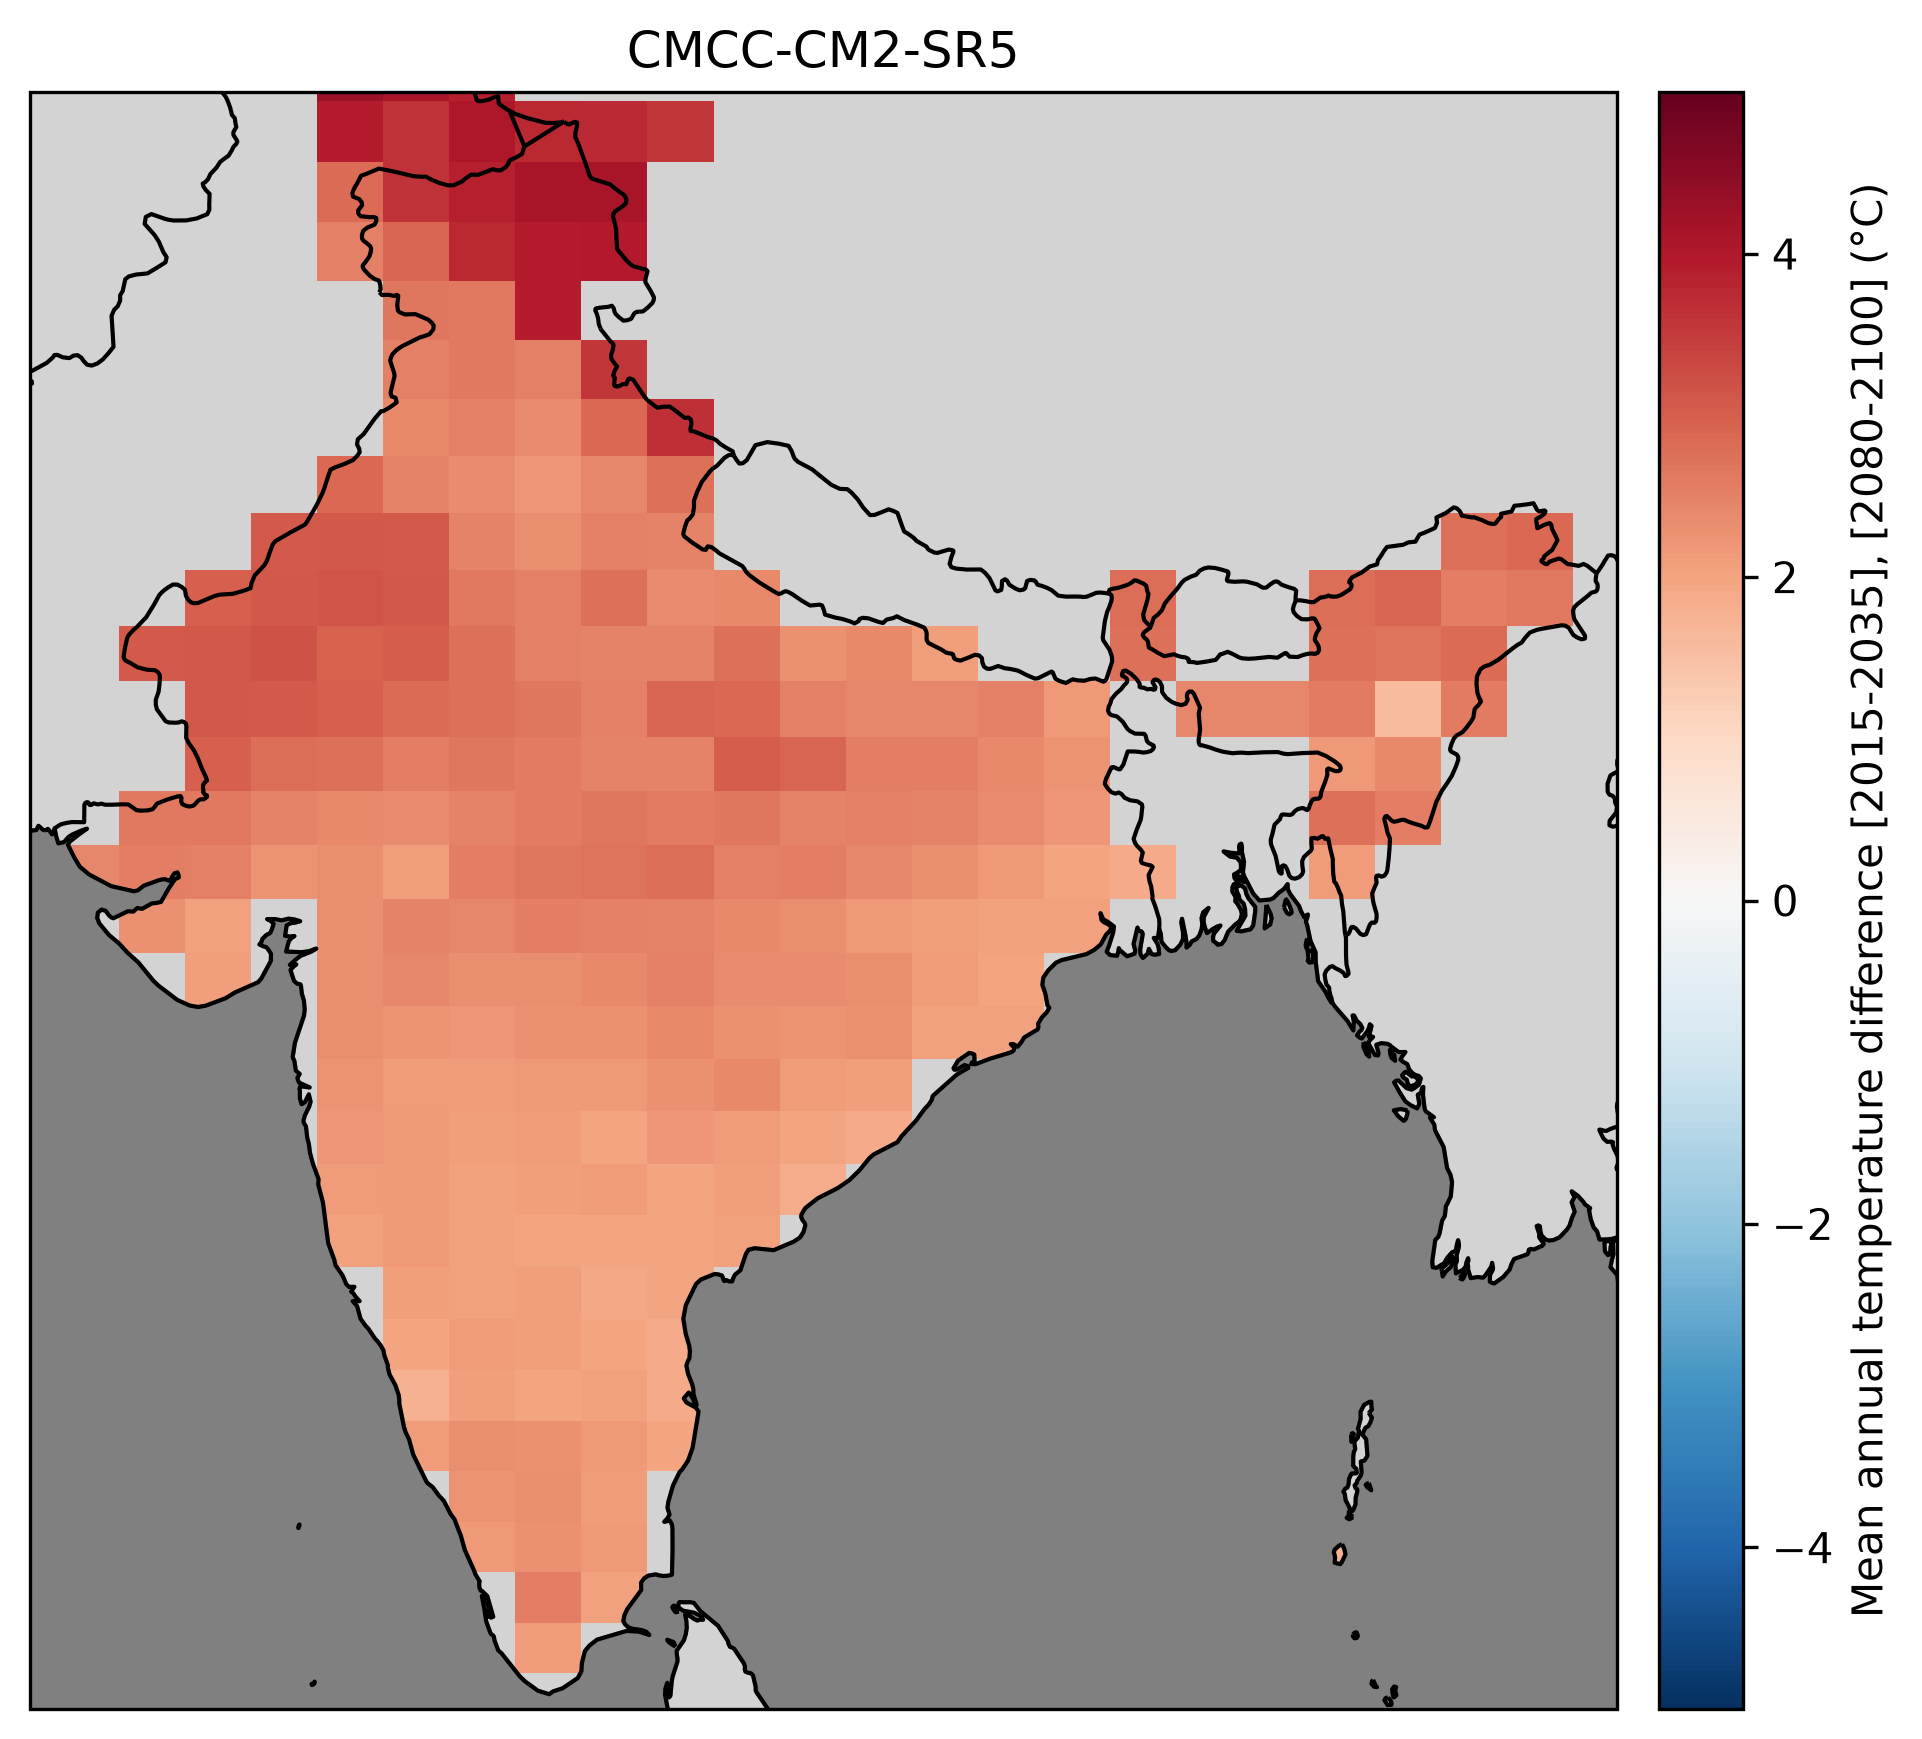
\includegraphics[width=0.32\columnwidth]{figures/annual_difference_ssp3_7_0_cmcc_cm2_sr5.png}
      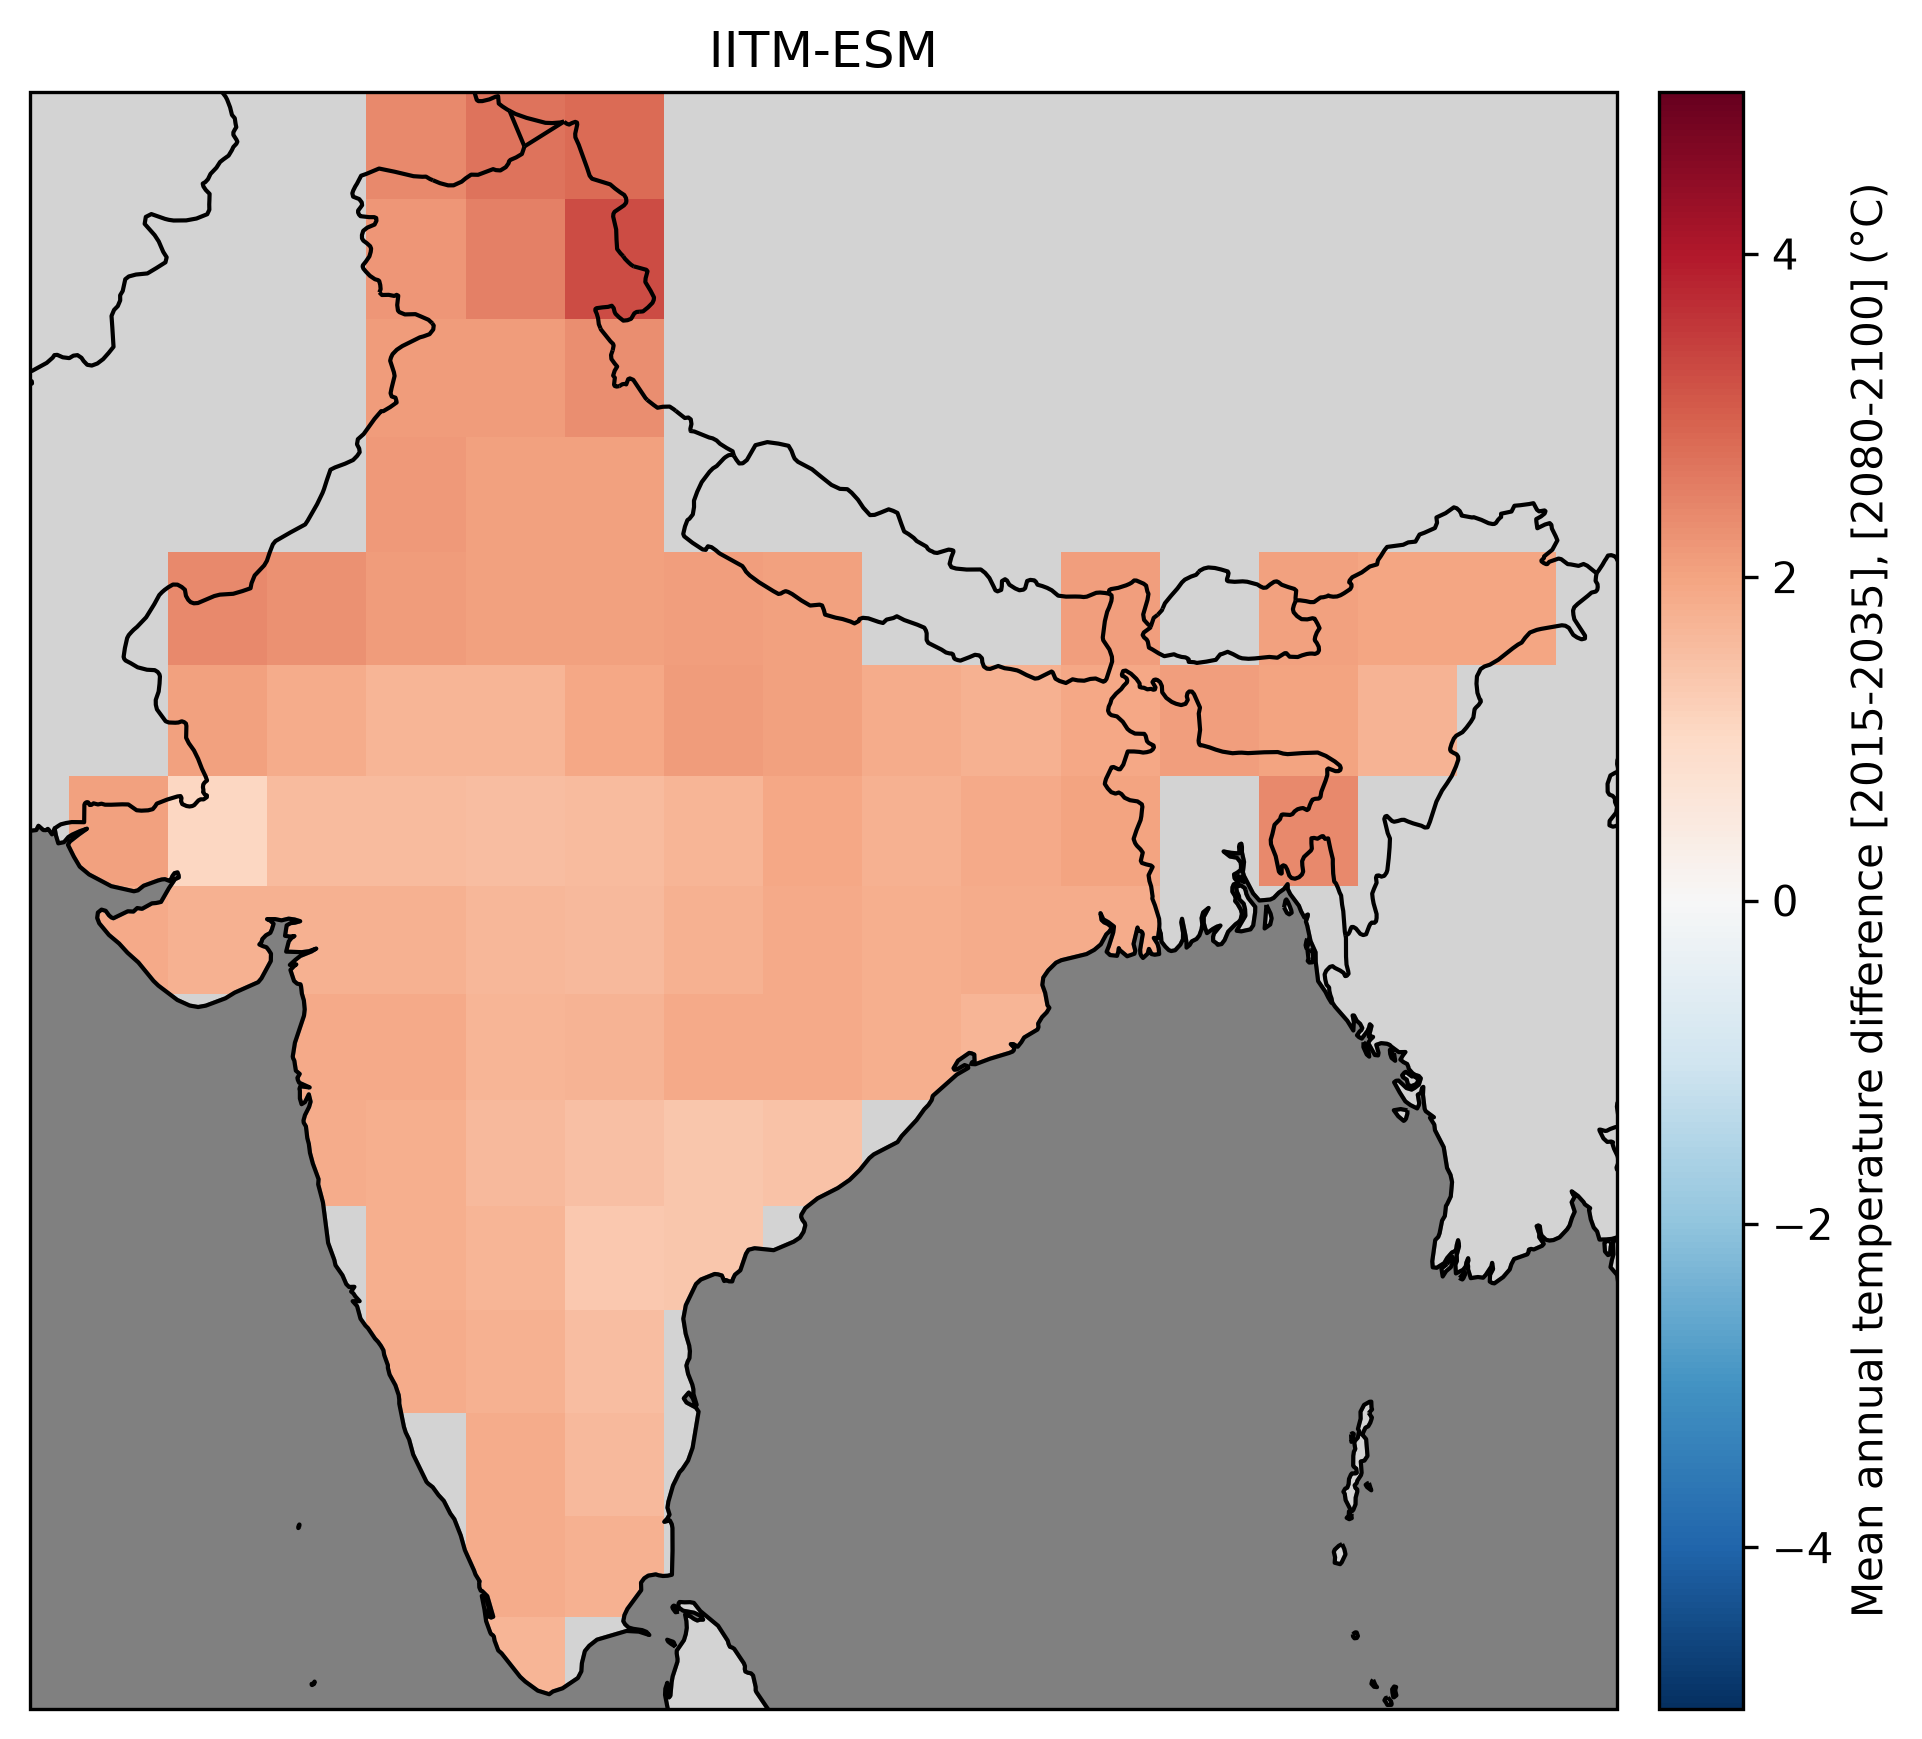
\includegraphics[width=0.32\columnwidth]{figures/annual_difference_ssp3_7_0_iitm_esm.png}
      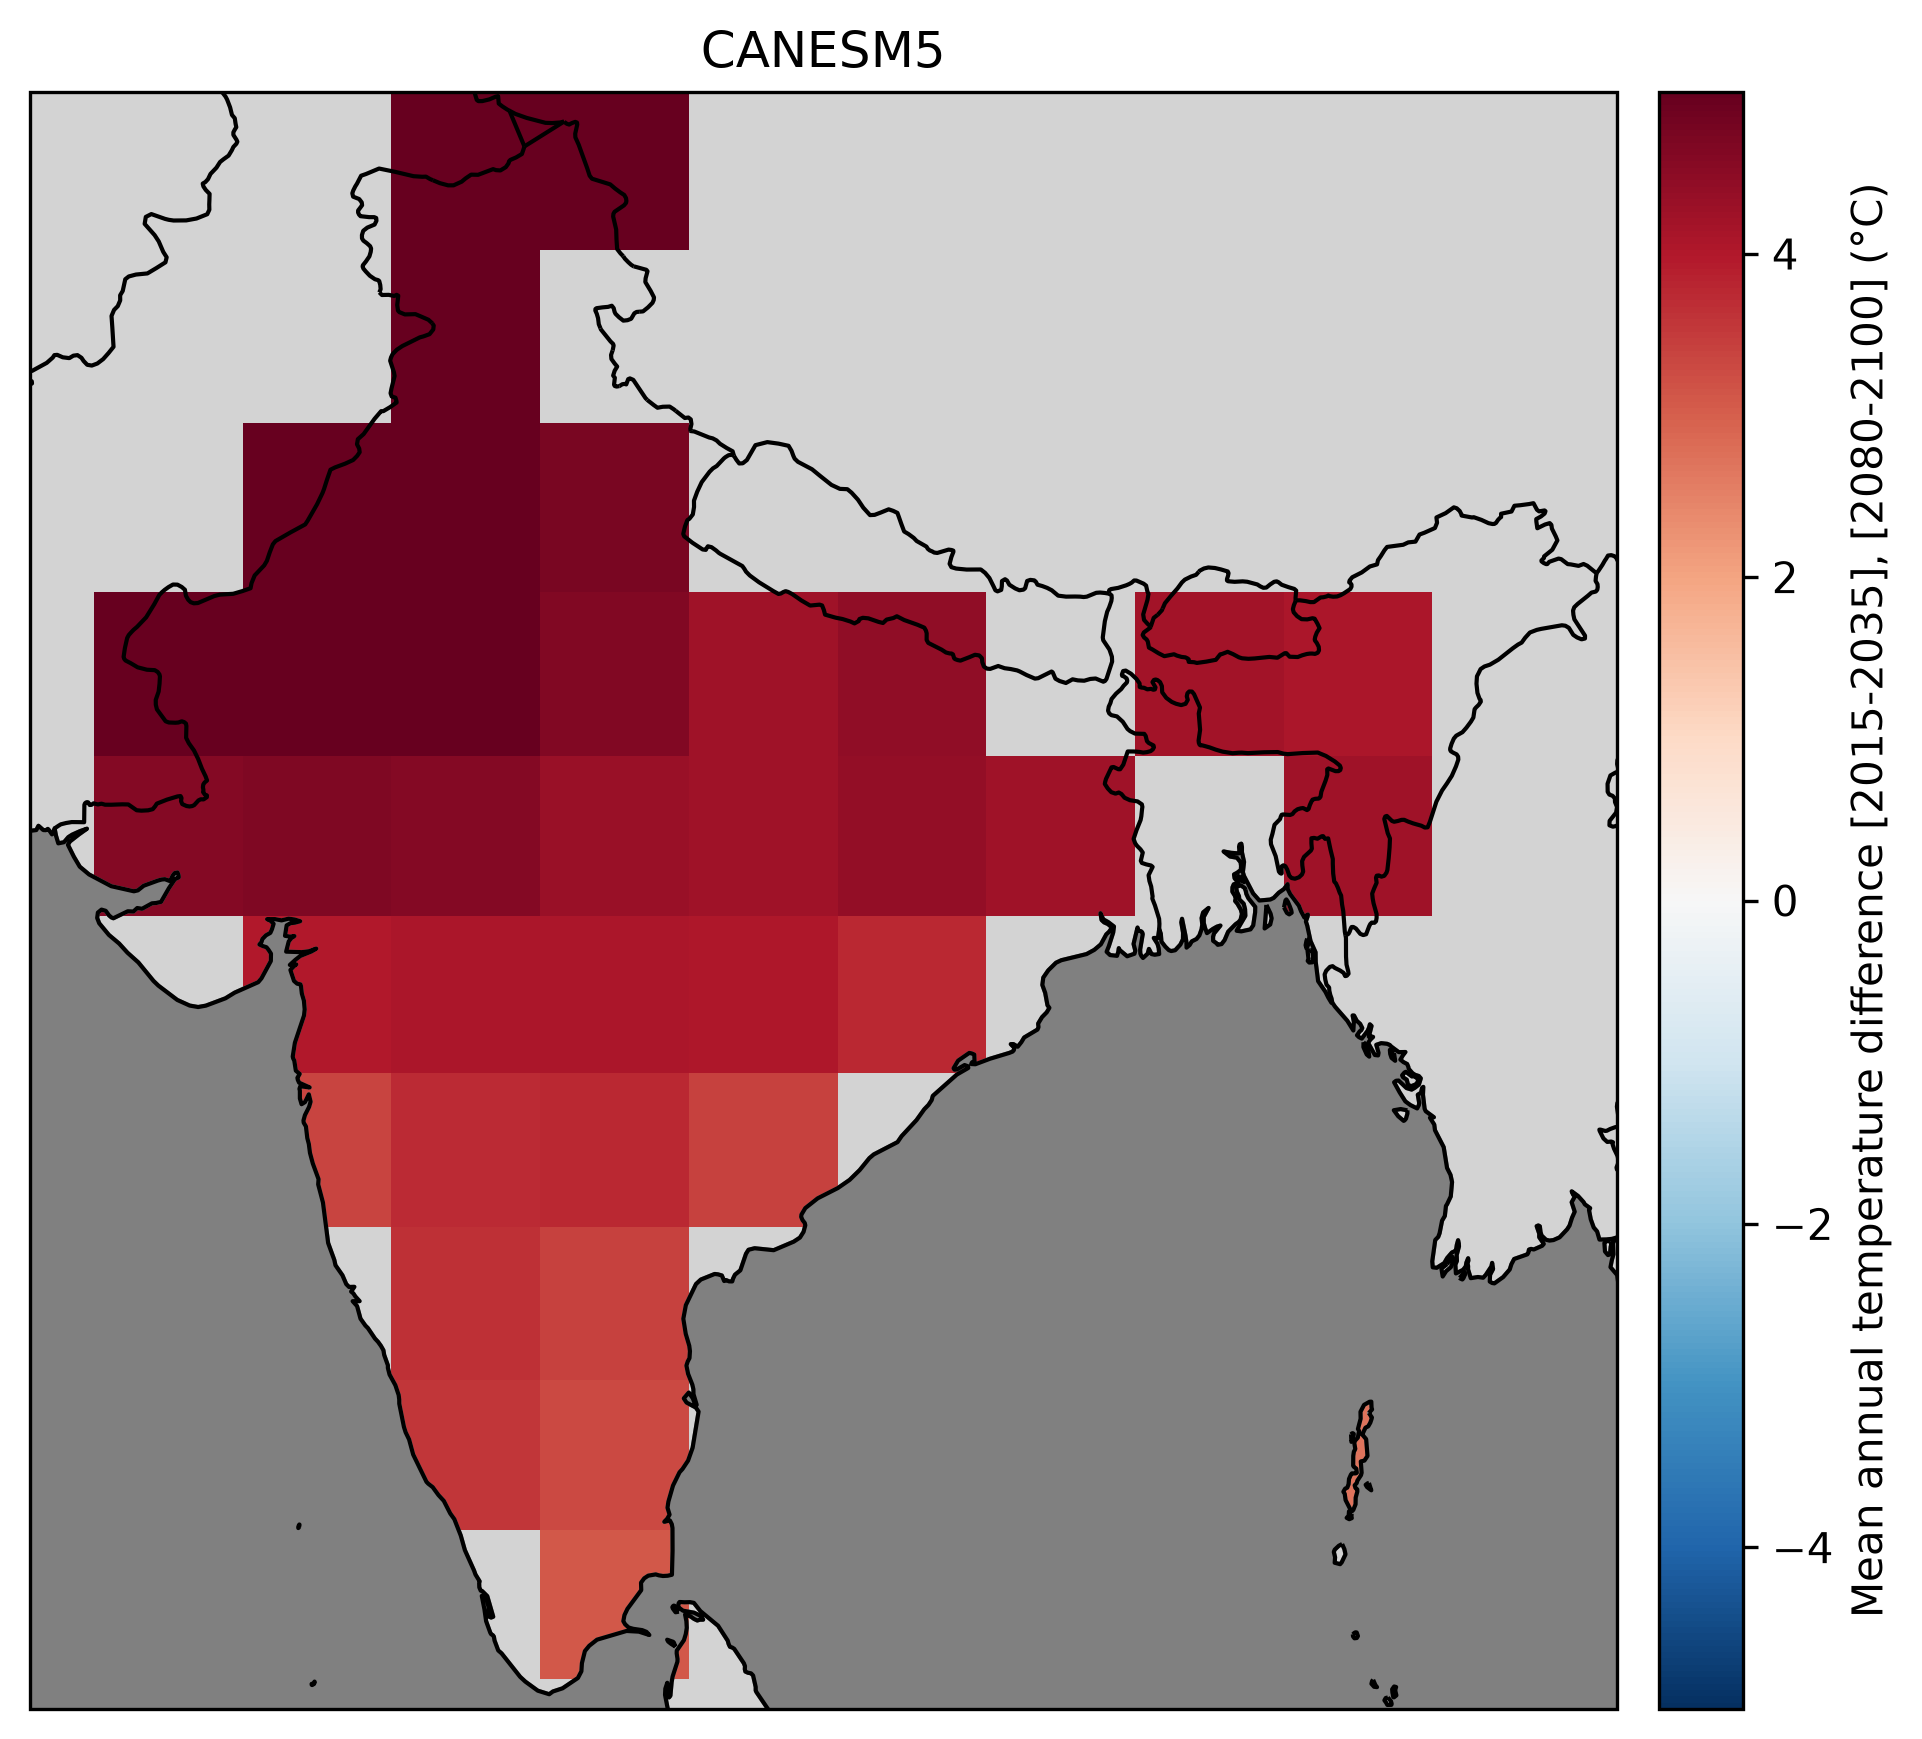
\includegraphics[width=0.32\columnwidth]{figures/annual_difference_ssp3_7_0_canesm5.png}\\
      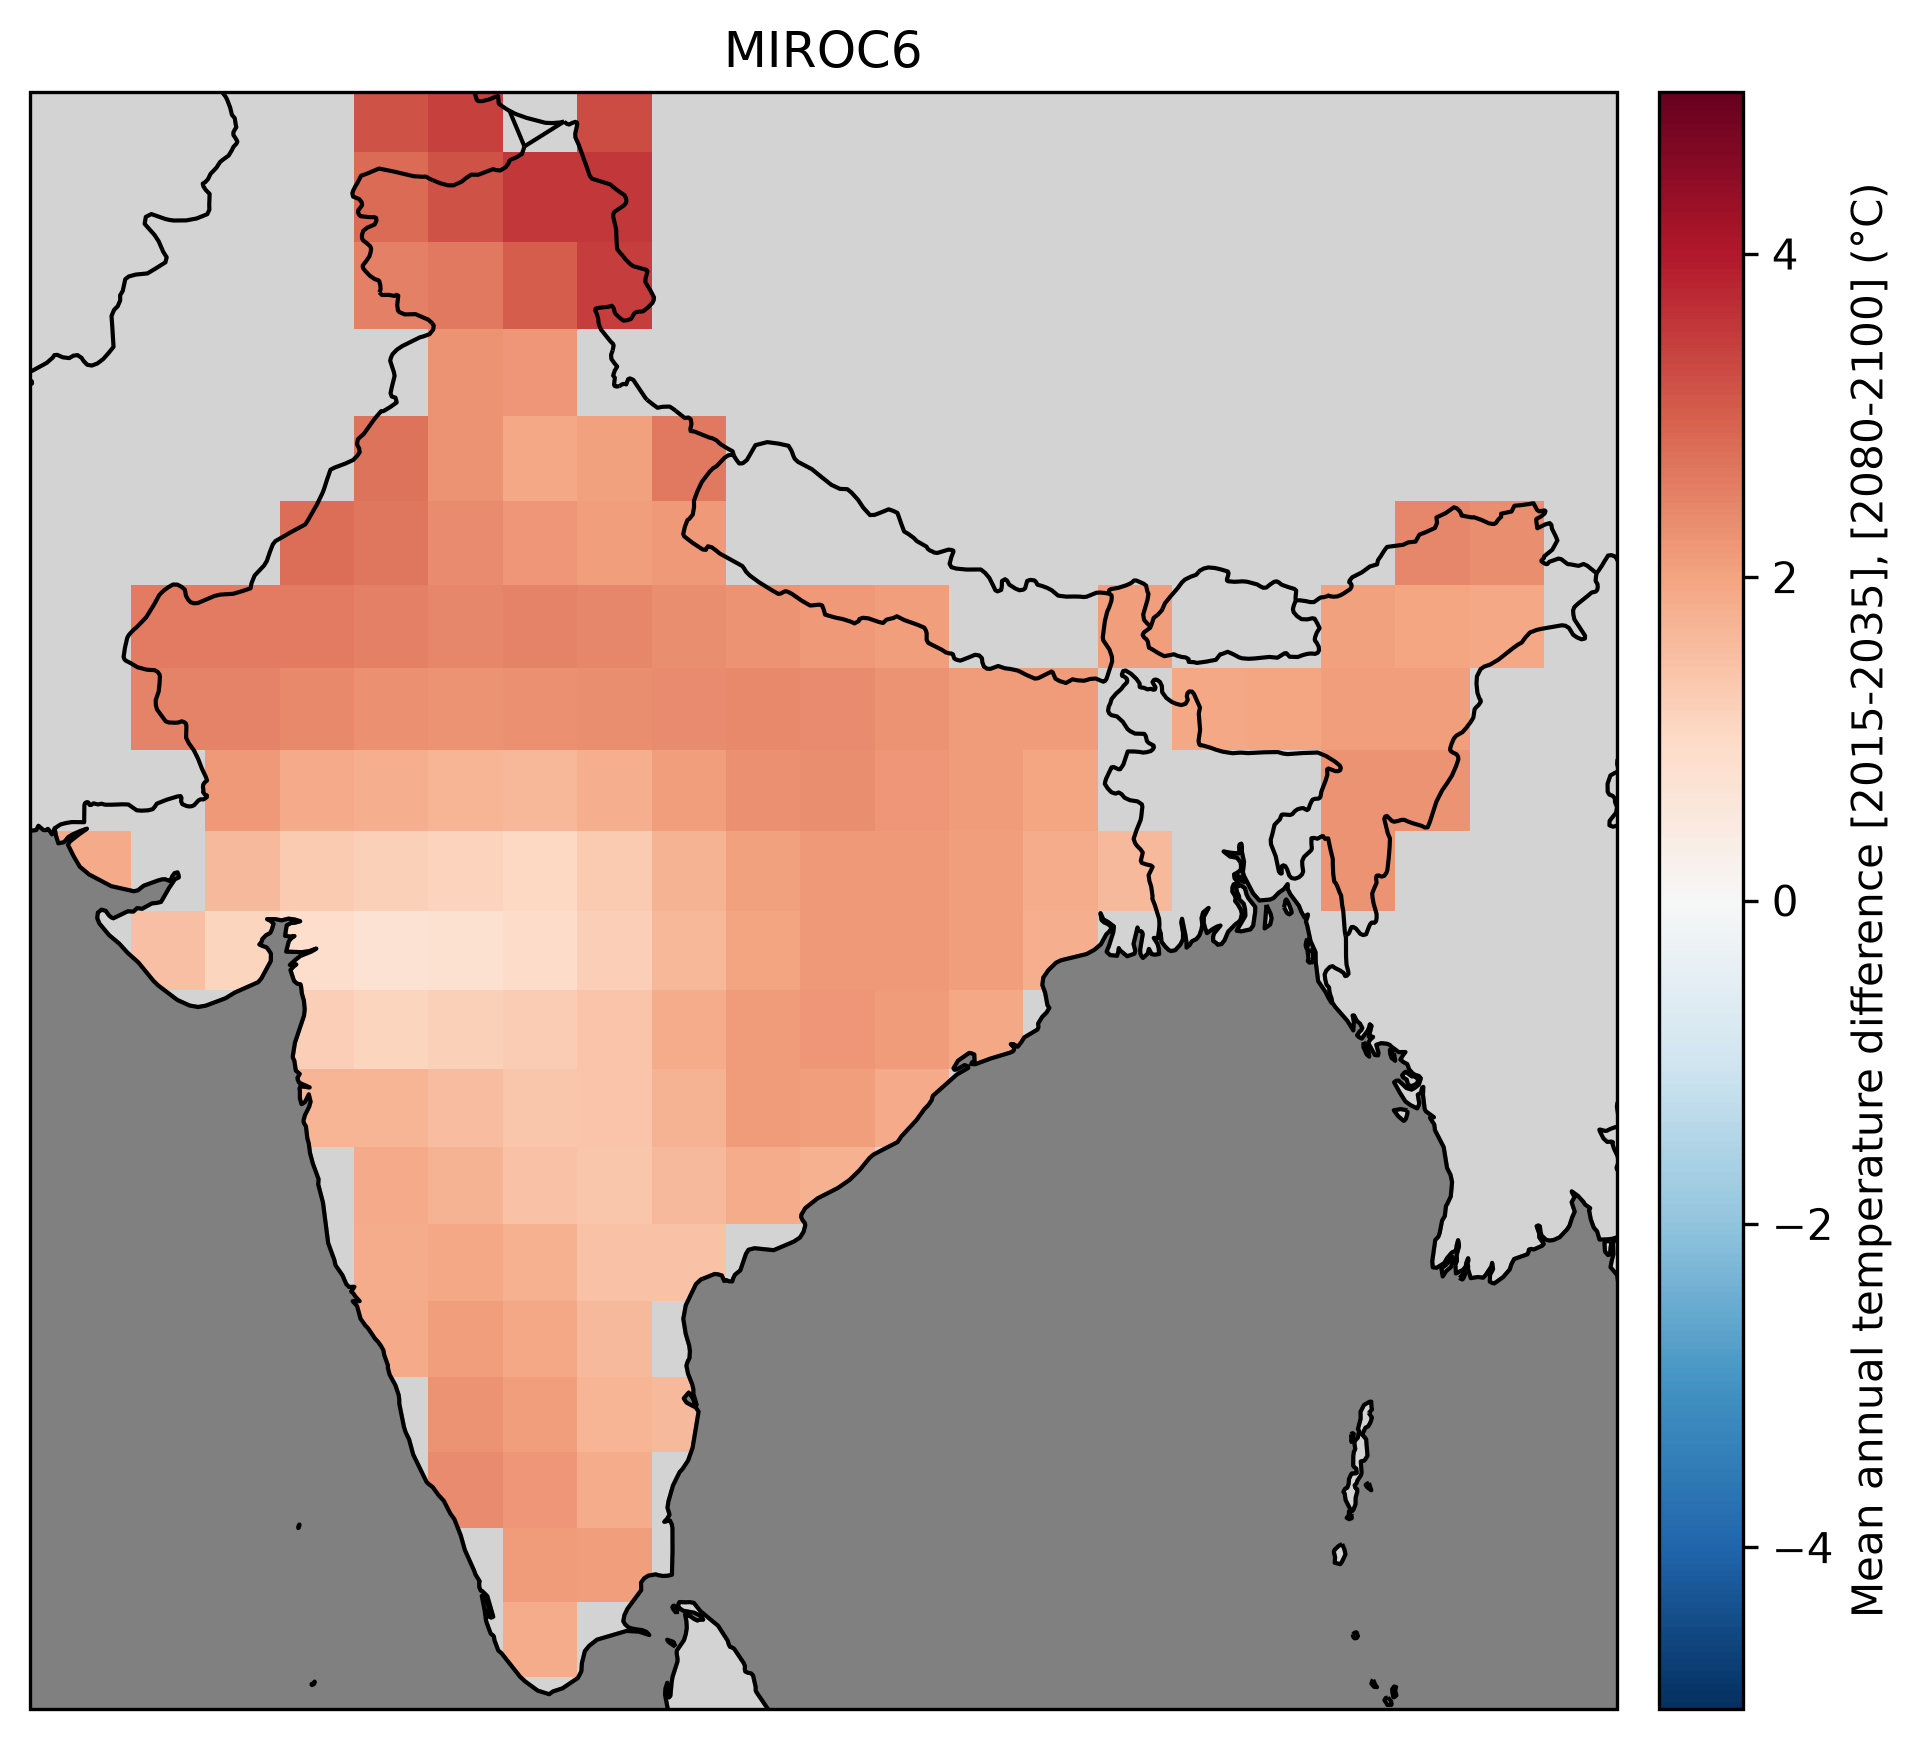
\includegraphics[width=0.32\columnwidth]{figures/annual_difference_ssp3_7_0_miroc6.png}
      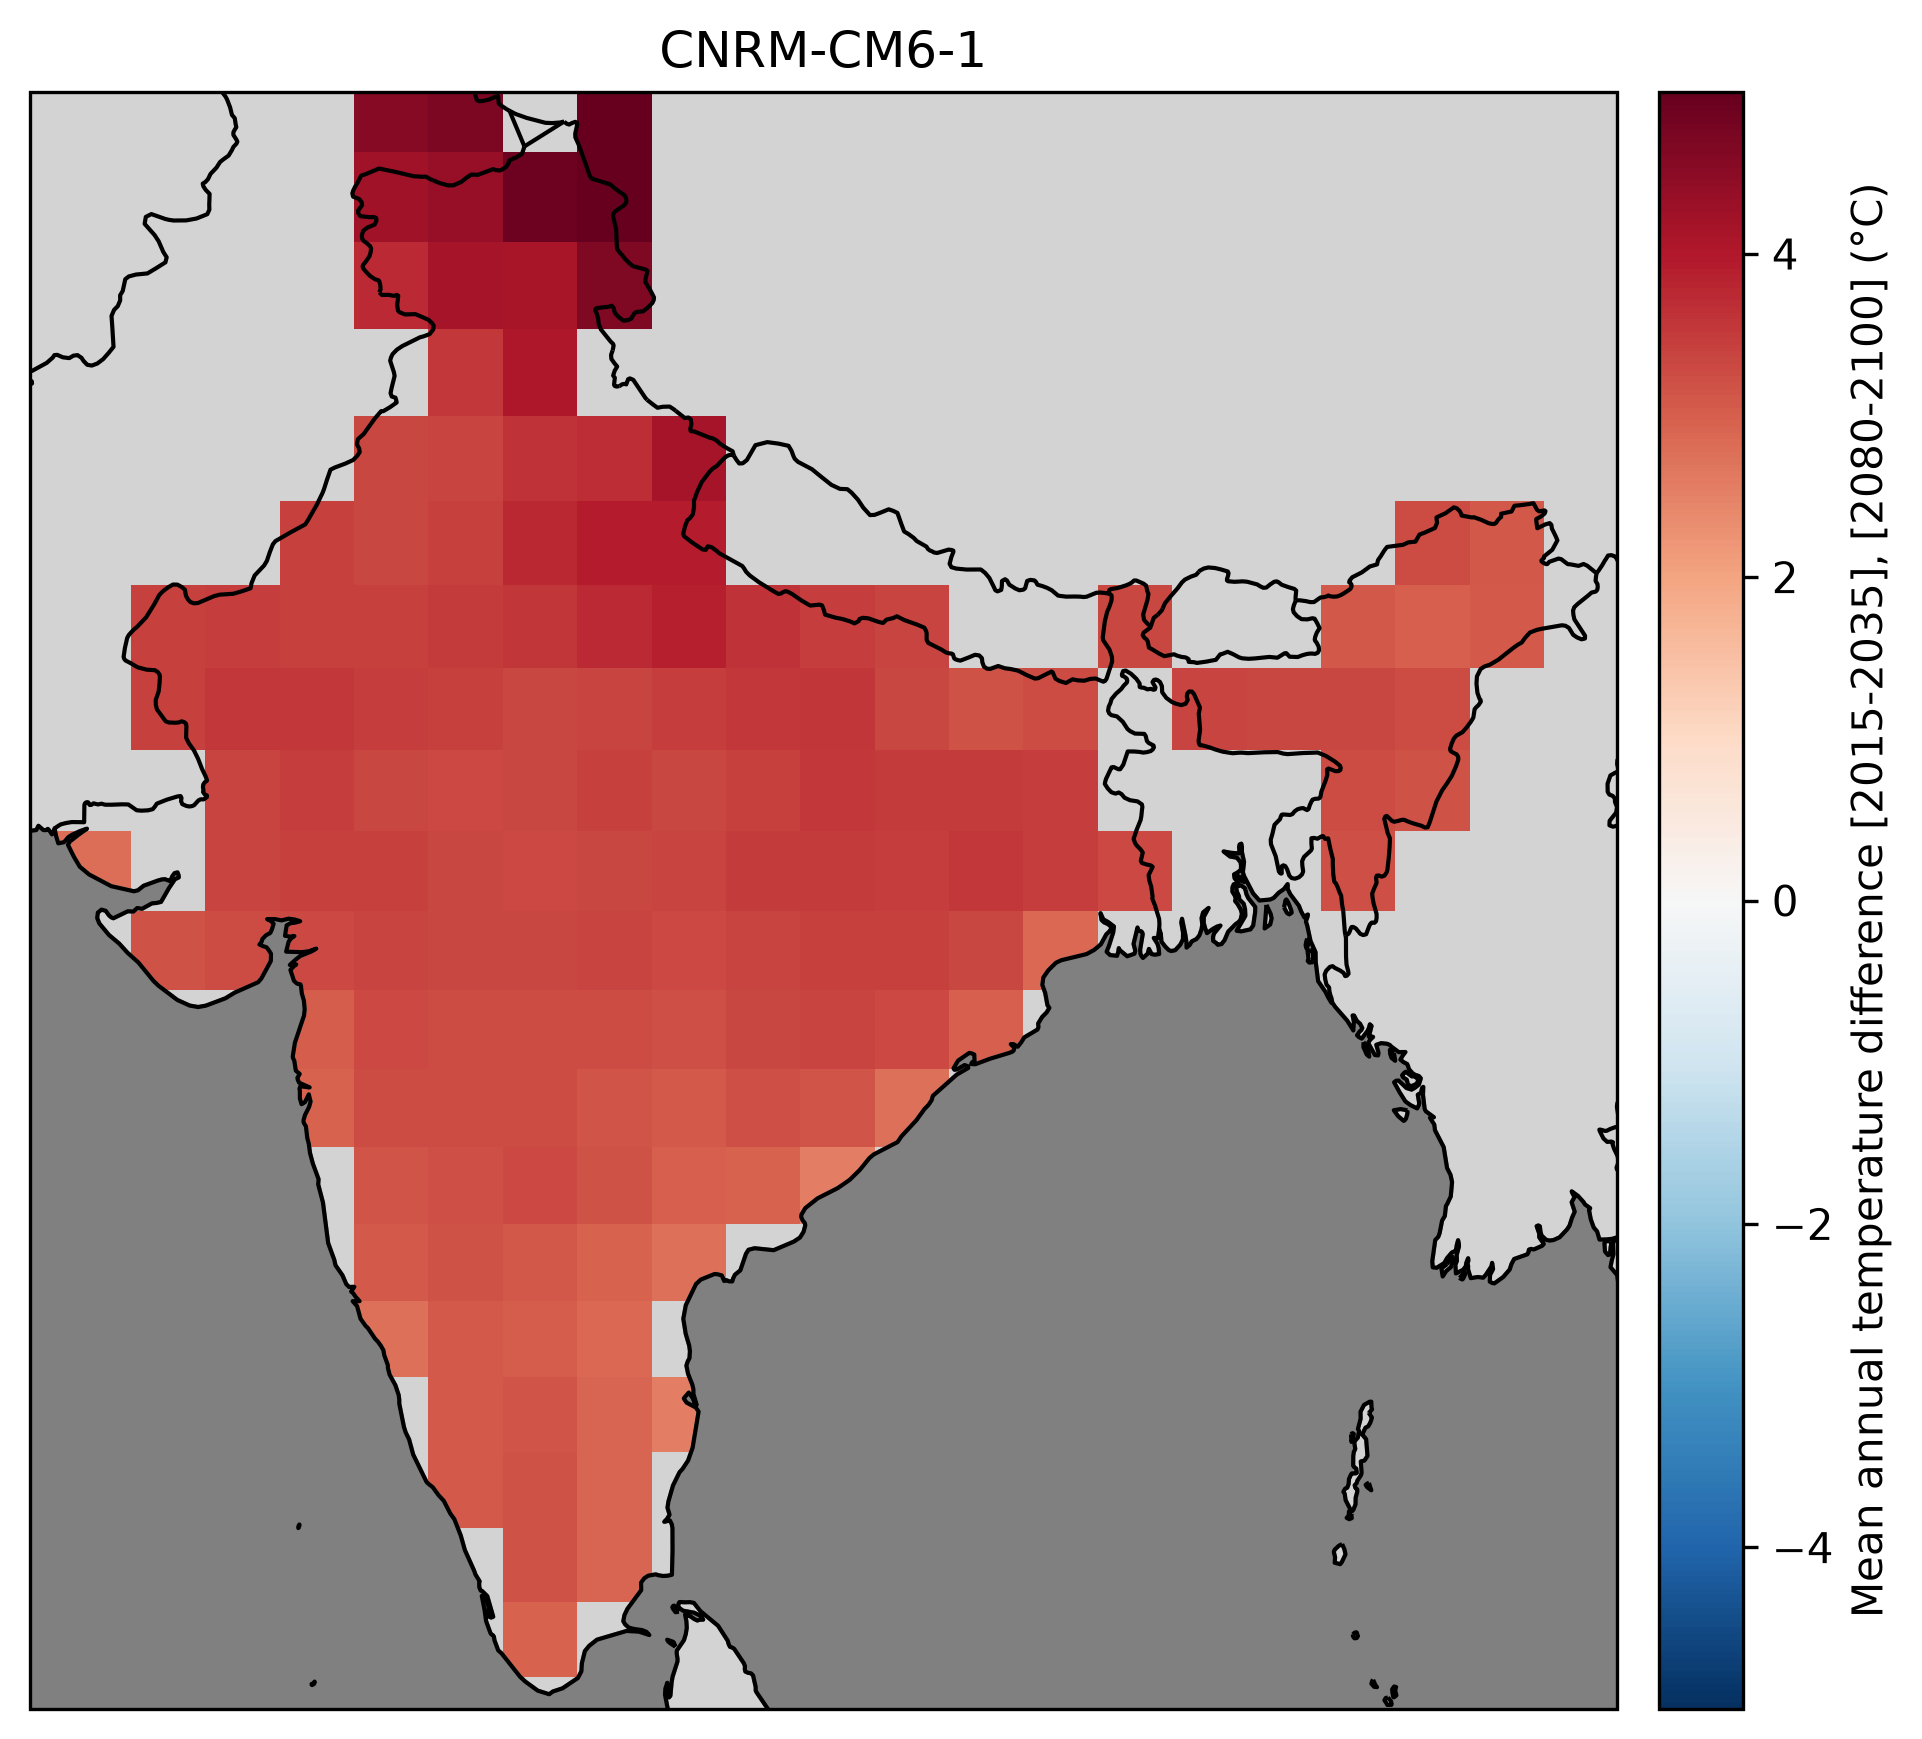
\includegraphics[width=0.32\columnwidth]{figures/annual_difference_ssp3_7_0_cnrm_cm6_1.png}
      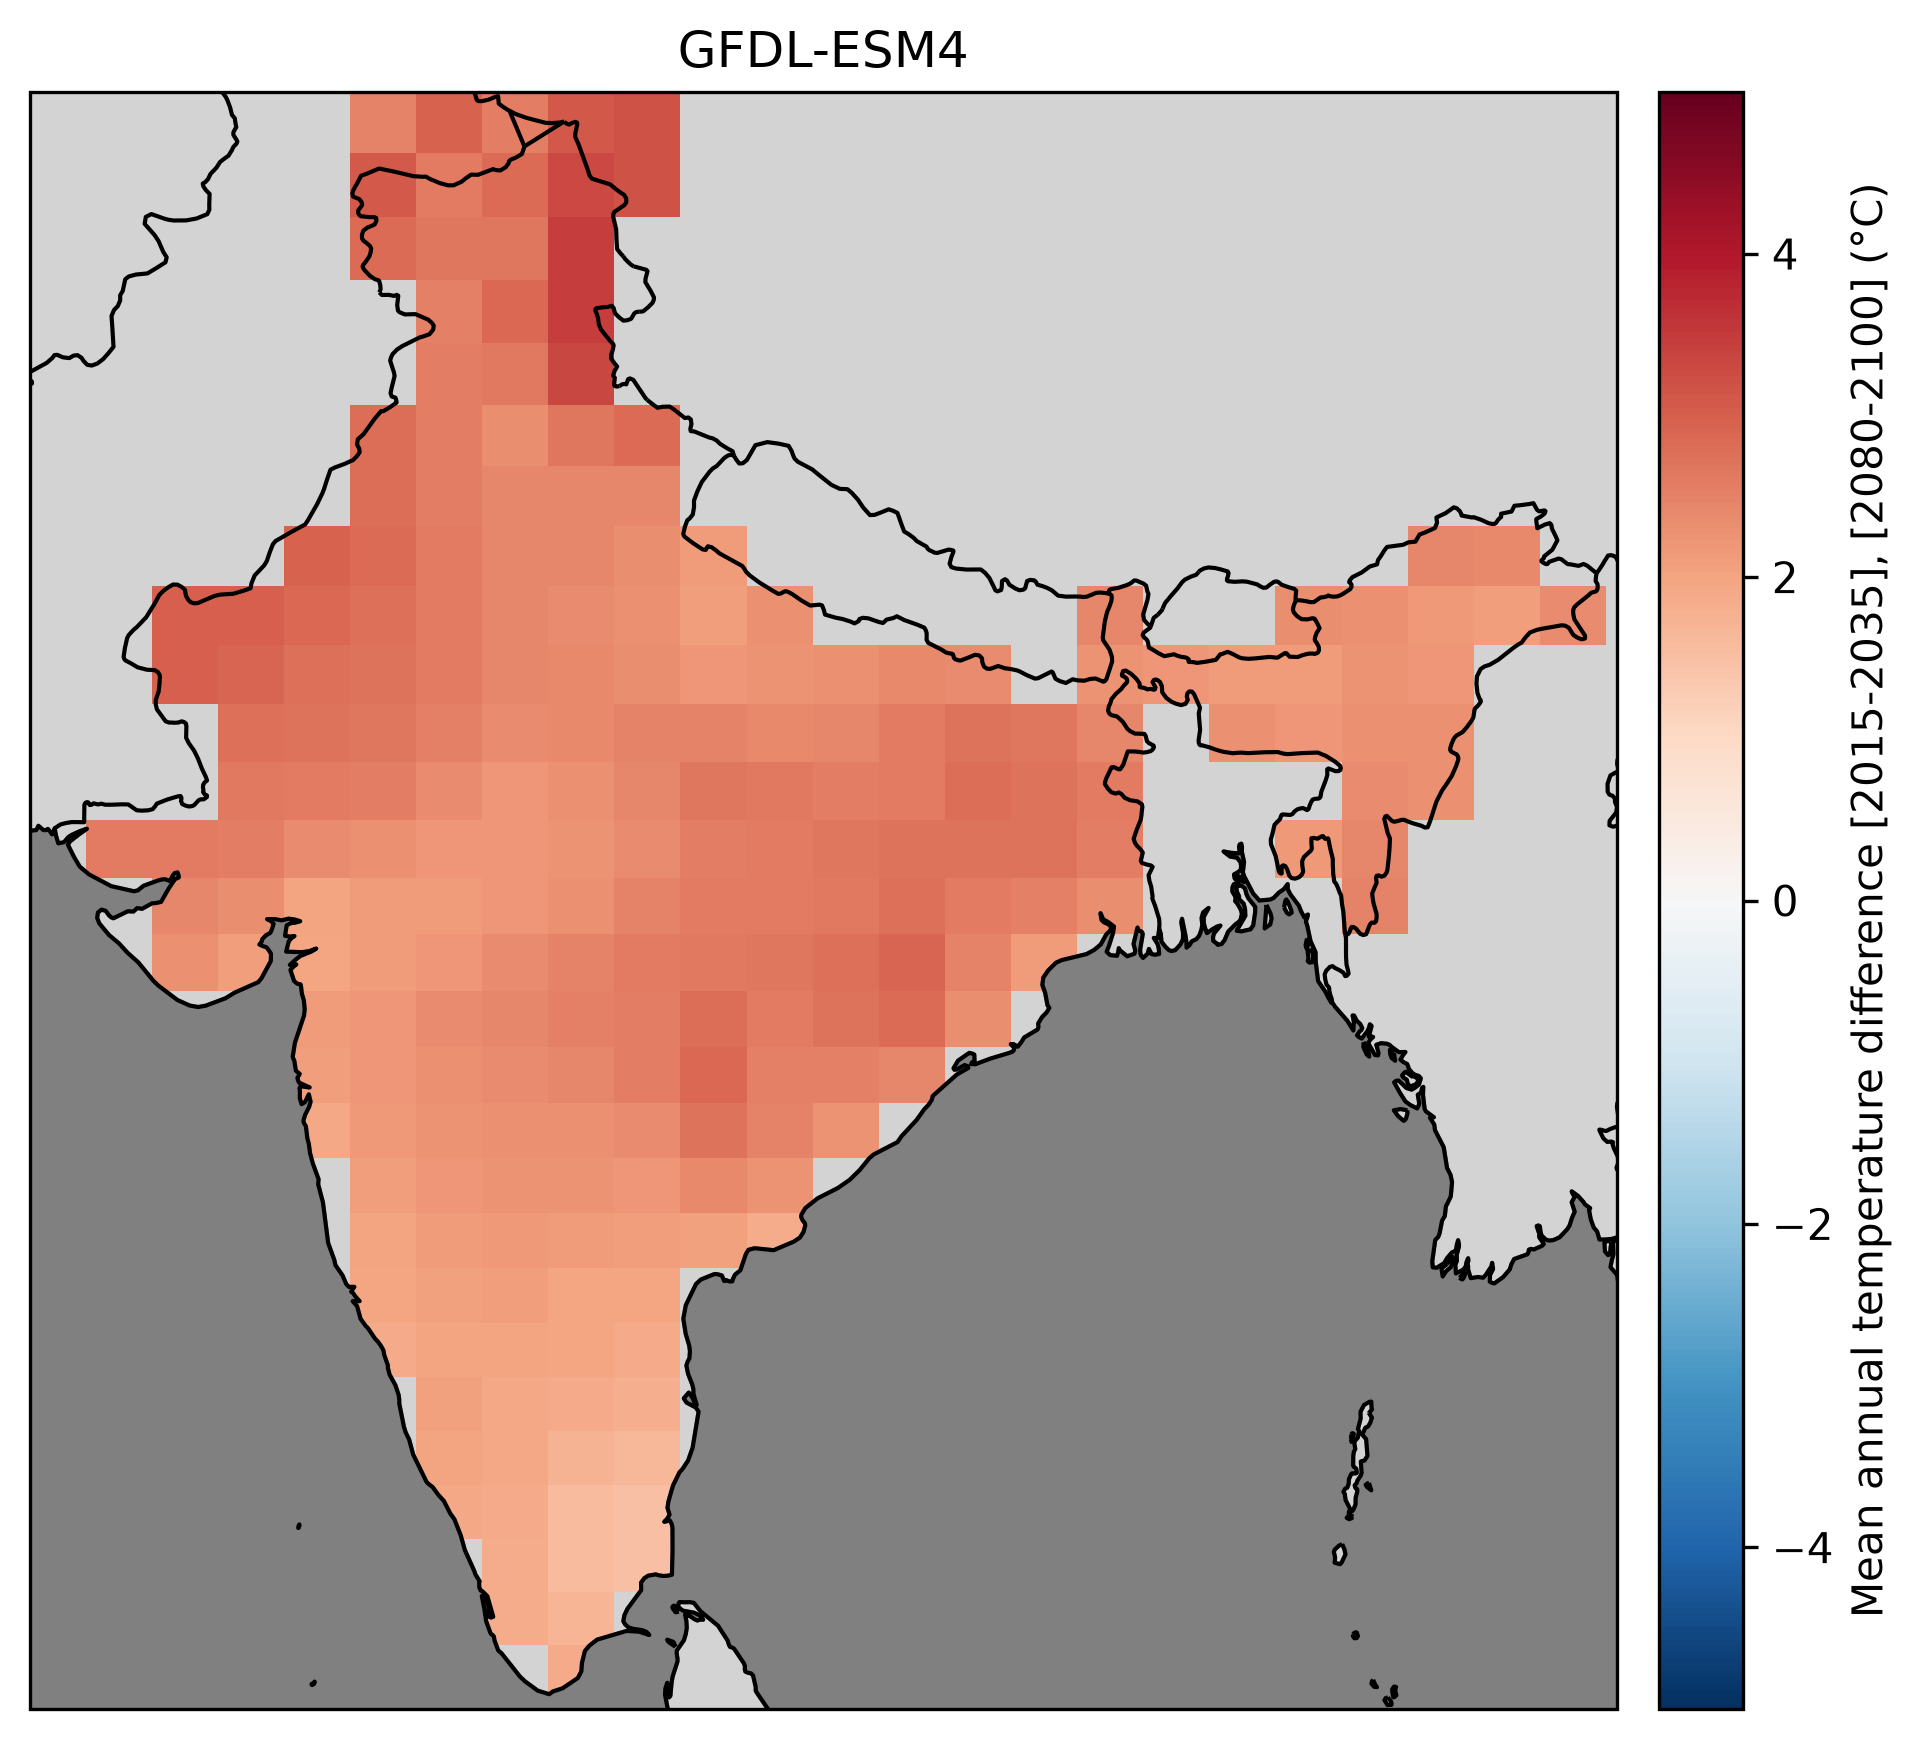
\includegraphics[width=0.32\columnwidth]{figures/annual_difference_ssp3_7_0_gfdl_esm4.png}
      \caption{\label{fig:map_diff_temp} Cartes des différences de températures moyennes annuelles entre 2015-2035 et 2080-2100 pour le scénario SSP3-7.0}
   \end{figure}

   \subsection{Calcul des CDD26}

   À partir des données géographiques des températures journalières de 2015 à 2100, nous calculons des moyennes pondérées par la distribution de population pour chaque état de l'Inde (\cite{ciesin_gridded_2017}). Les frontières des différents états et la répartition de la population sont illustrées \ref{fig:map_population}. Ainsi, on supppose que la répartition de la population reste constante dans le temps. \\

   \begin{figure}[ht]
   \centering
      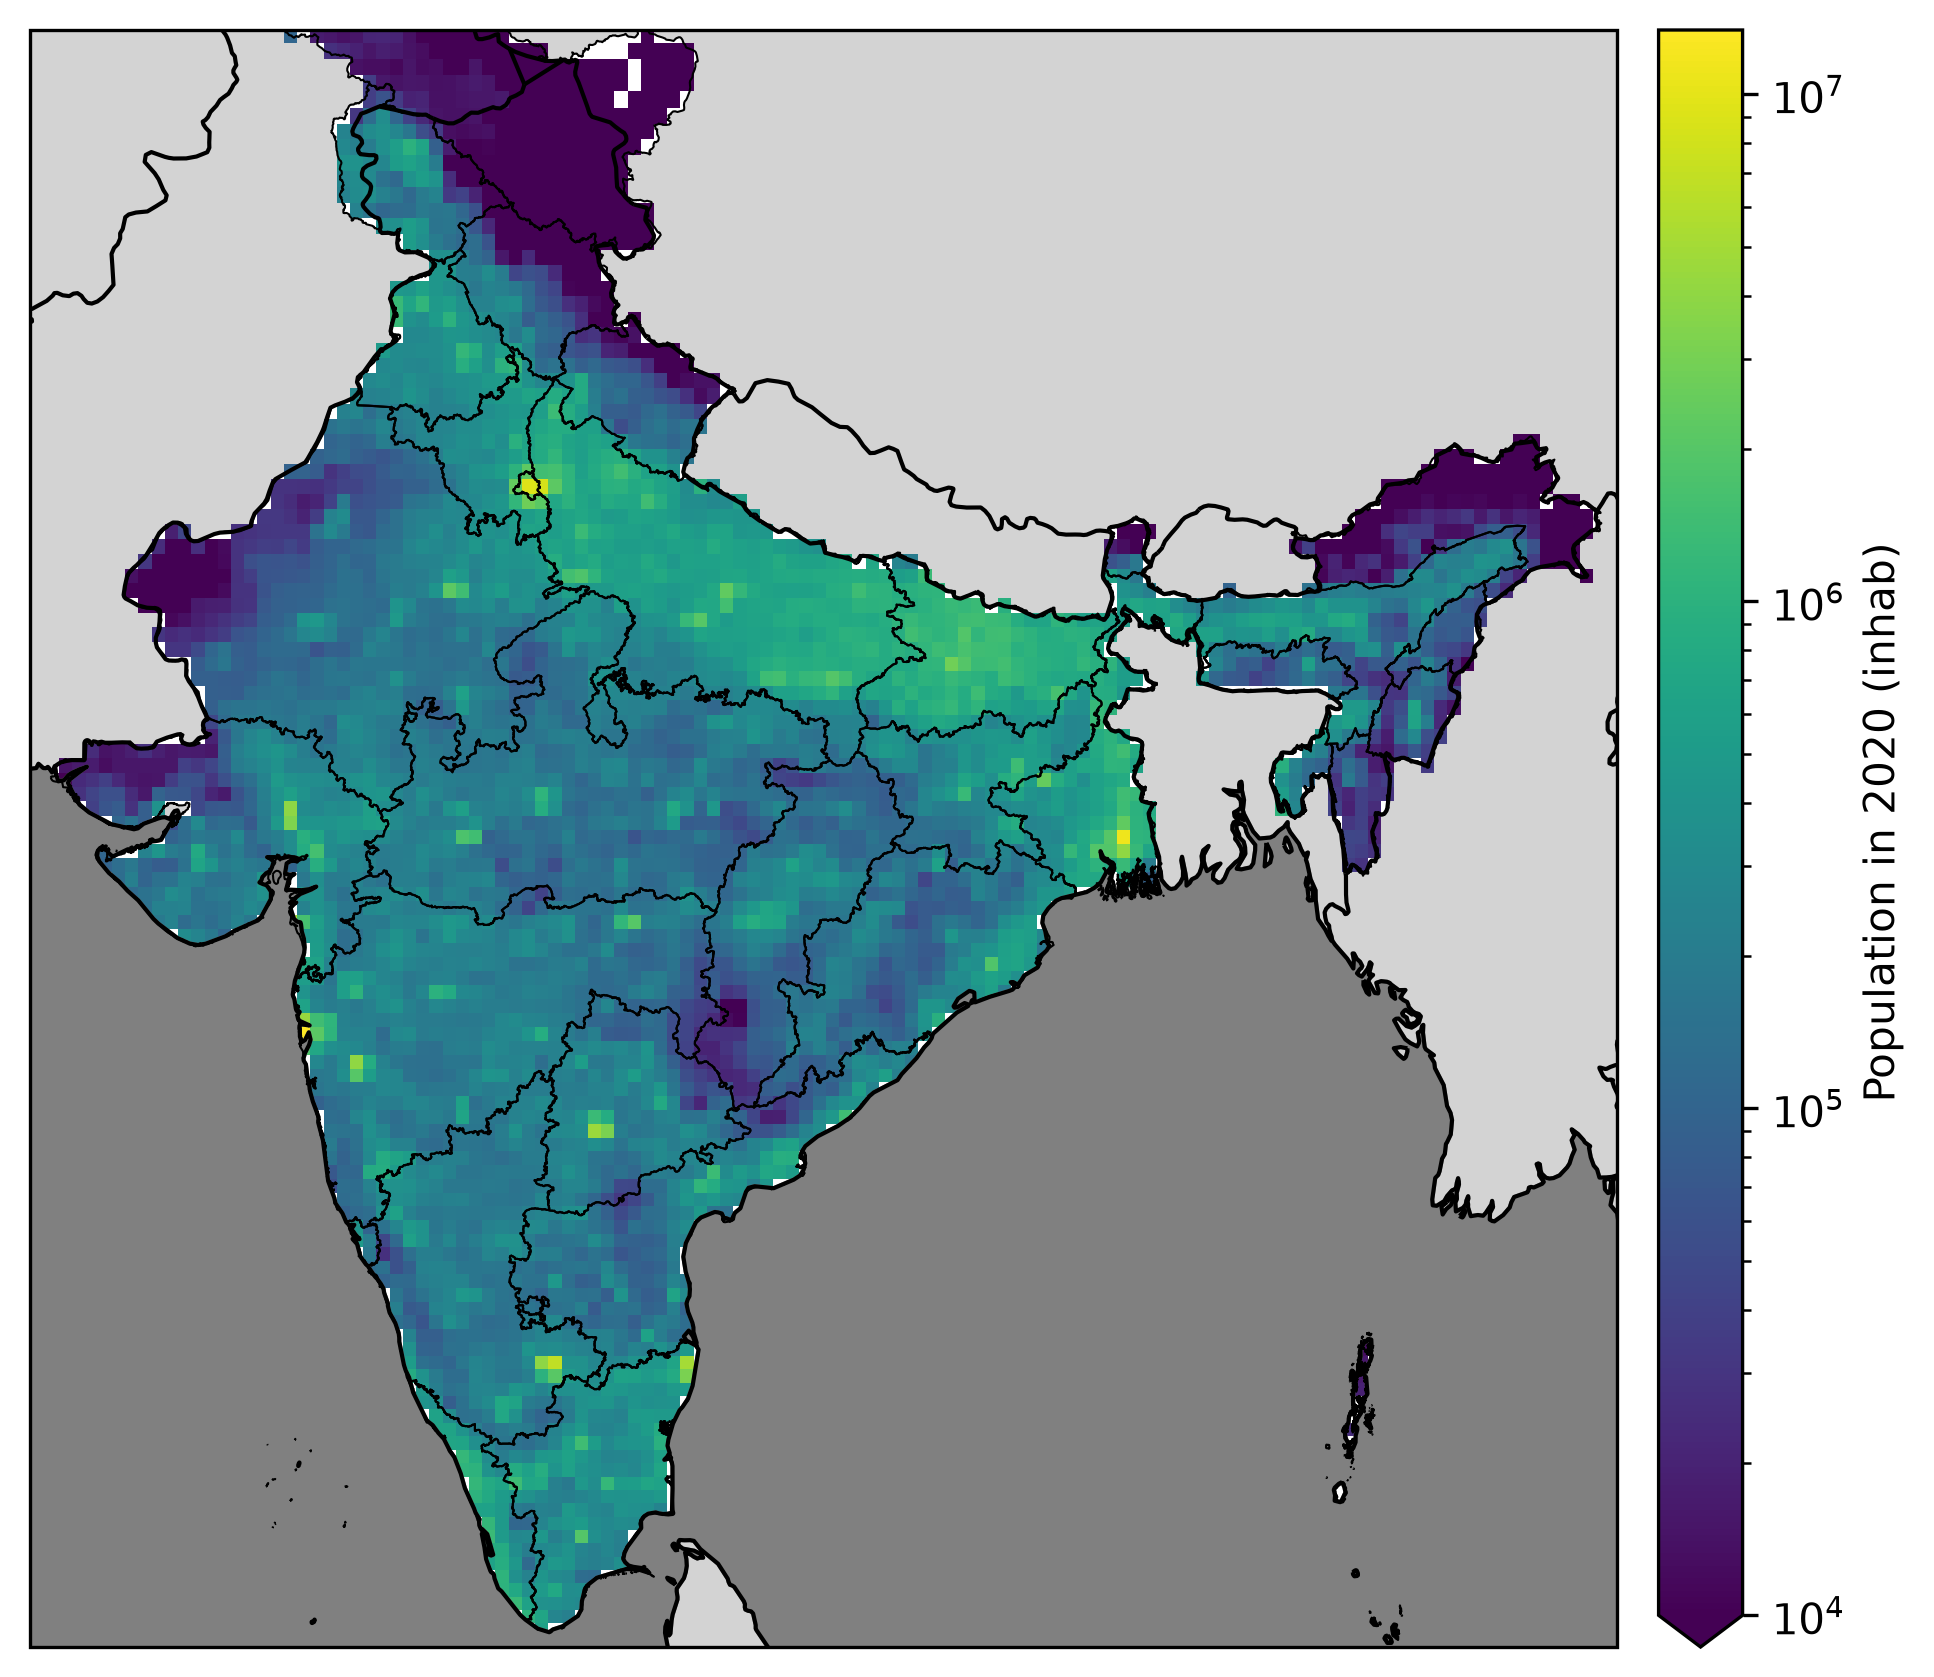
\includegraphics[width=0.49\columnwidth]{figures/map_population.png}
      \caption{\label{fig:map_population} Carte des états et de la population en Inde en 2020}
   \end{figure}

   Le passage des températures journalières aux CDD26 d'une année $y$ se fait d'après l'équation \eqref{eq:cdd}.

   \begin{equation}
      \label{eq:cdd}
      \mathrm{CDD26}(y) = \sum_{d\in y} \left(\bar{T}_d - 26\right)^+
   \end{equation}

   Les valeurs de CDD26 pour chaque état et chaque modèle climatique sont ensuite recalées sur les données historiques de CDD26 (\cite{iea_weather_2023}), utilisées pour la caractérisation des taux d'équipement en climatisation. Les valeurs de recalage (somme ou soustraction d'une valeur constante) sont disponibles dans le fichier \texttt{data/cdd\_calibration.csv} du dépôt git. 

   \subsection{Projection de CDD26}

   On obtient alors les projections de CDD26 par état, de 2015 à 2100, pour chaque scénario et chaque modèle climatique. Les valeurs sont disponibles dans le fichier \texttt{data/AC\_projection.csv} du dépôt git. Les graphes par état sont présentés en annexe de ce document (\ref{sec:projections_par_etat}). À titre d'illustration, la \ref{fig:proj_cdd_india} représente l'évolution des CDD26 pondérés par la distribution de population pour l'ensemble de l'Inde.

   \begin{figure}[ht]
      \centering
      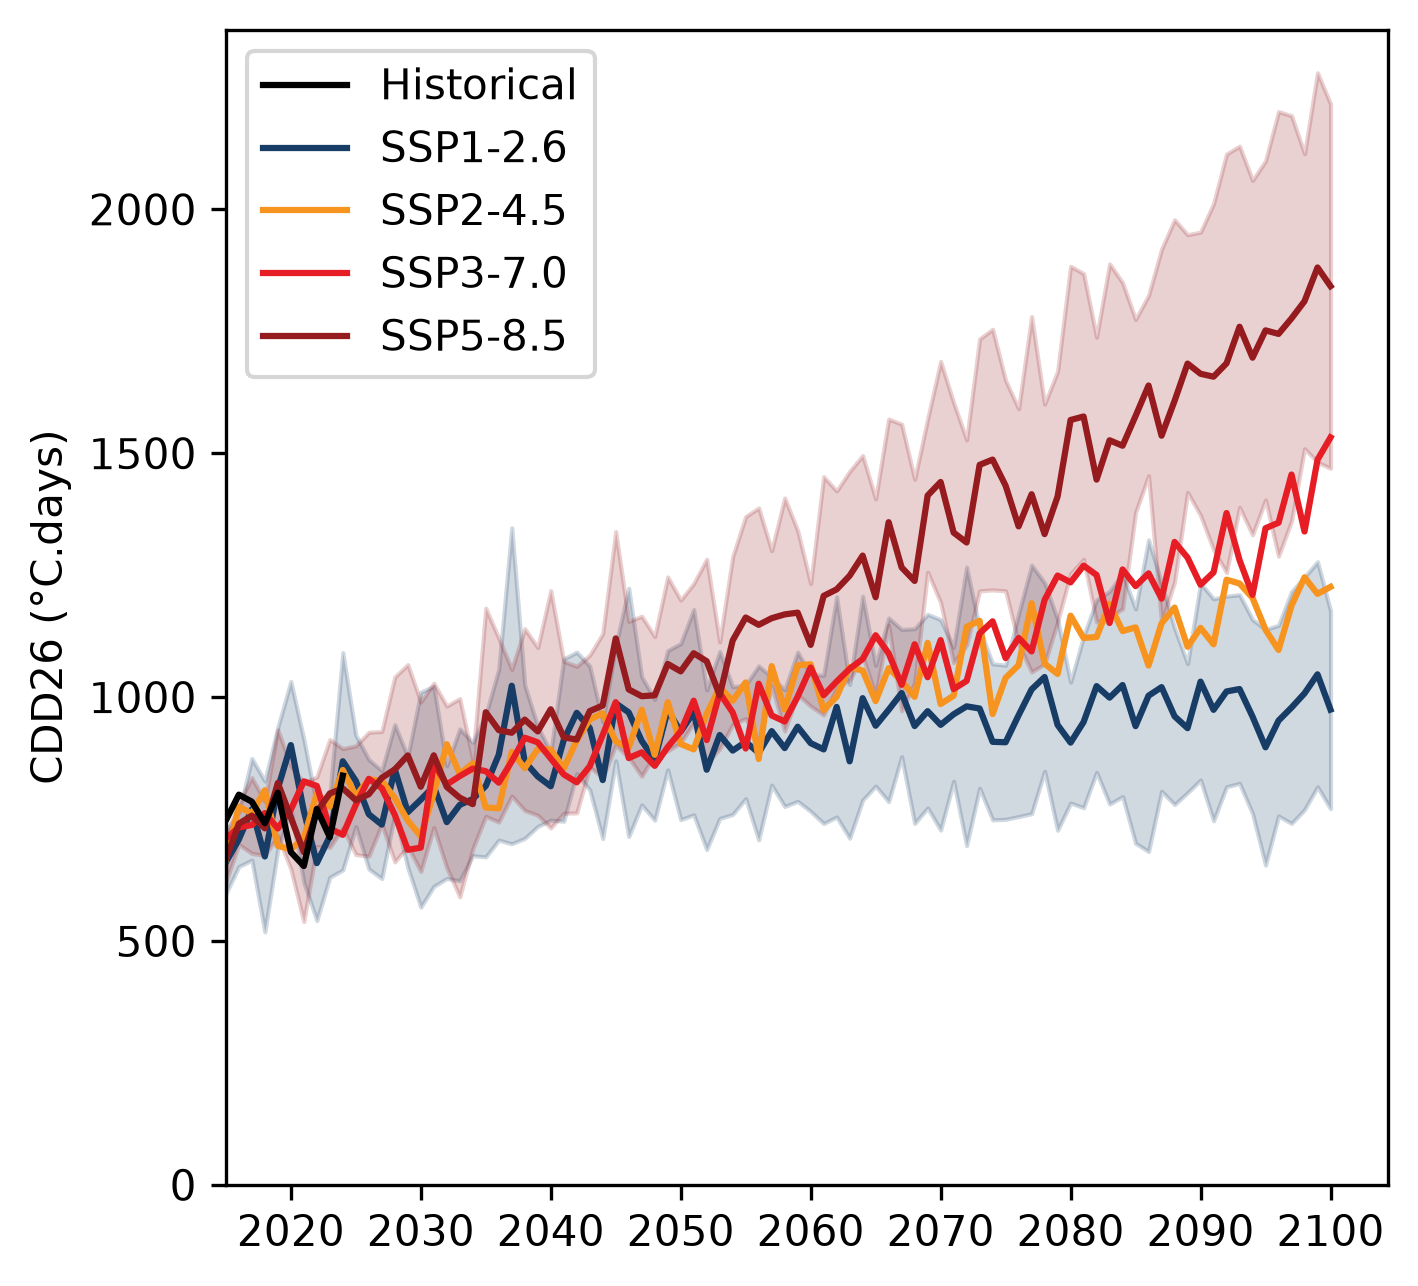
\includegraphics[width=0.49\columnwidth]{figures/projection_cdd26_india.png}
      \caption{\label{fig:proj_cdd_india} Projections des CDD26 en Inde}
   \end{figure}


\section{Projections de PIB par habitant et de population}

Les données de projections de PIB par habitant (\cite{dellink_long-term_2017,k_c_updating_2024}) et de nombre d'habitants (\cite{kc_human_2017,k_c_updating_2024}) sont disponibles à l'échelle nationale, et sont téléchargées depuis la plateforme \textit{Scenario Explorer} (\cite{iiasa_shared_2026}). Les projections sont calibrées sur les données d'enquête de 2021 pour rester cohérent avec l'étape de caractérisation des taux d'équipement. On obtient les projections illustrées \ref{fig:proj_gdp_pop_india}.

   \begin{figure}[ht]
      \centering
      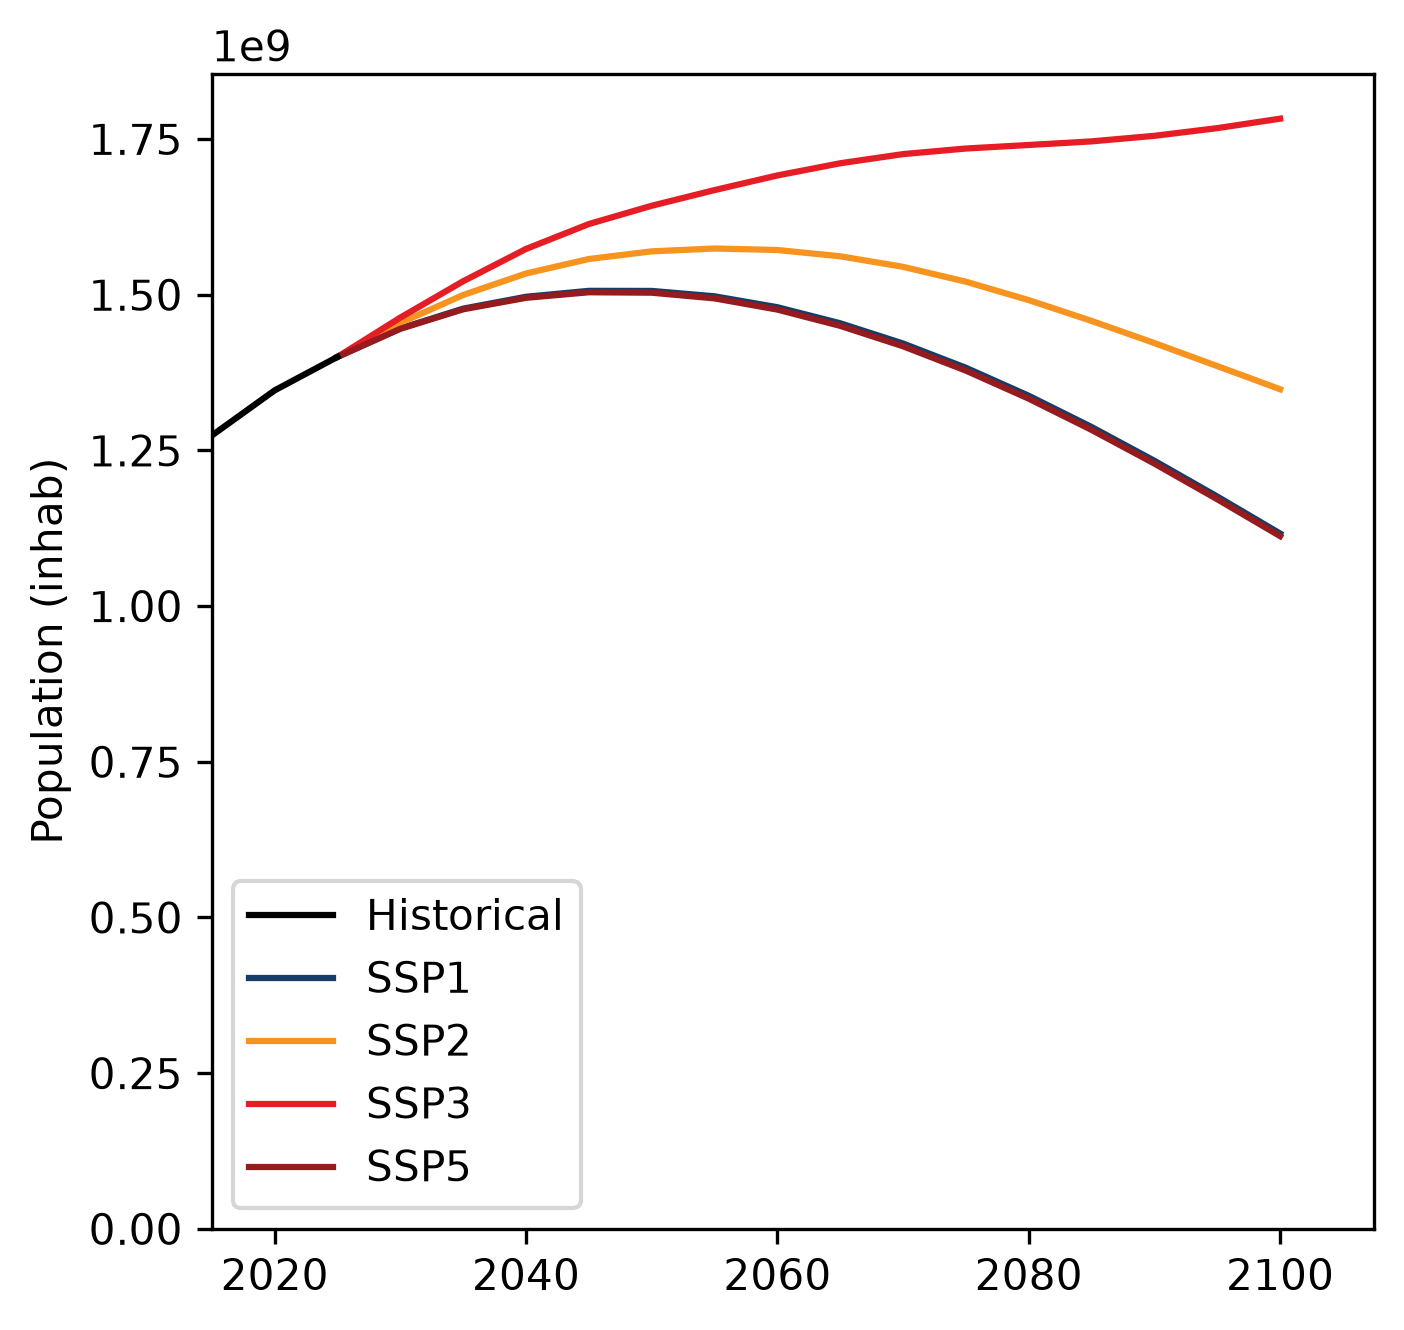
\includegraphics[width=0.49\columnwidth]{figures/projection_population_india.png}
      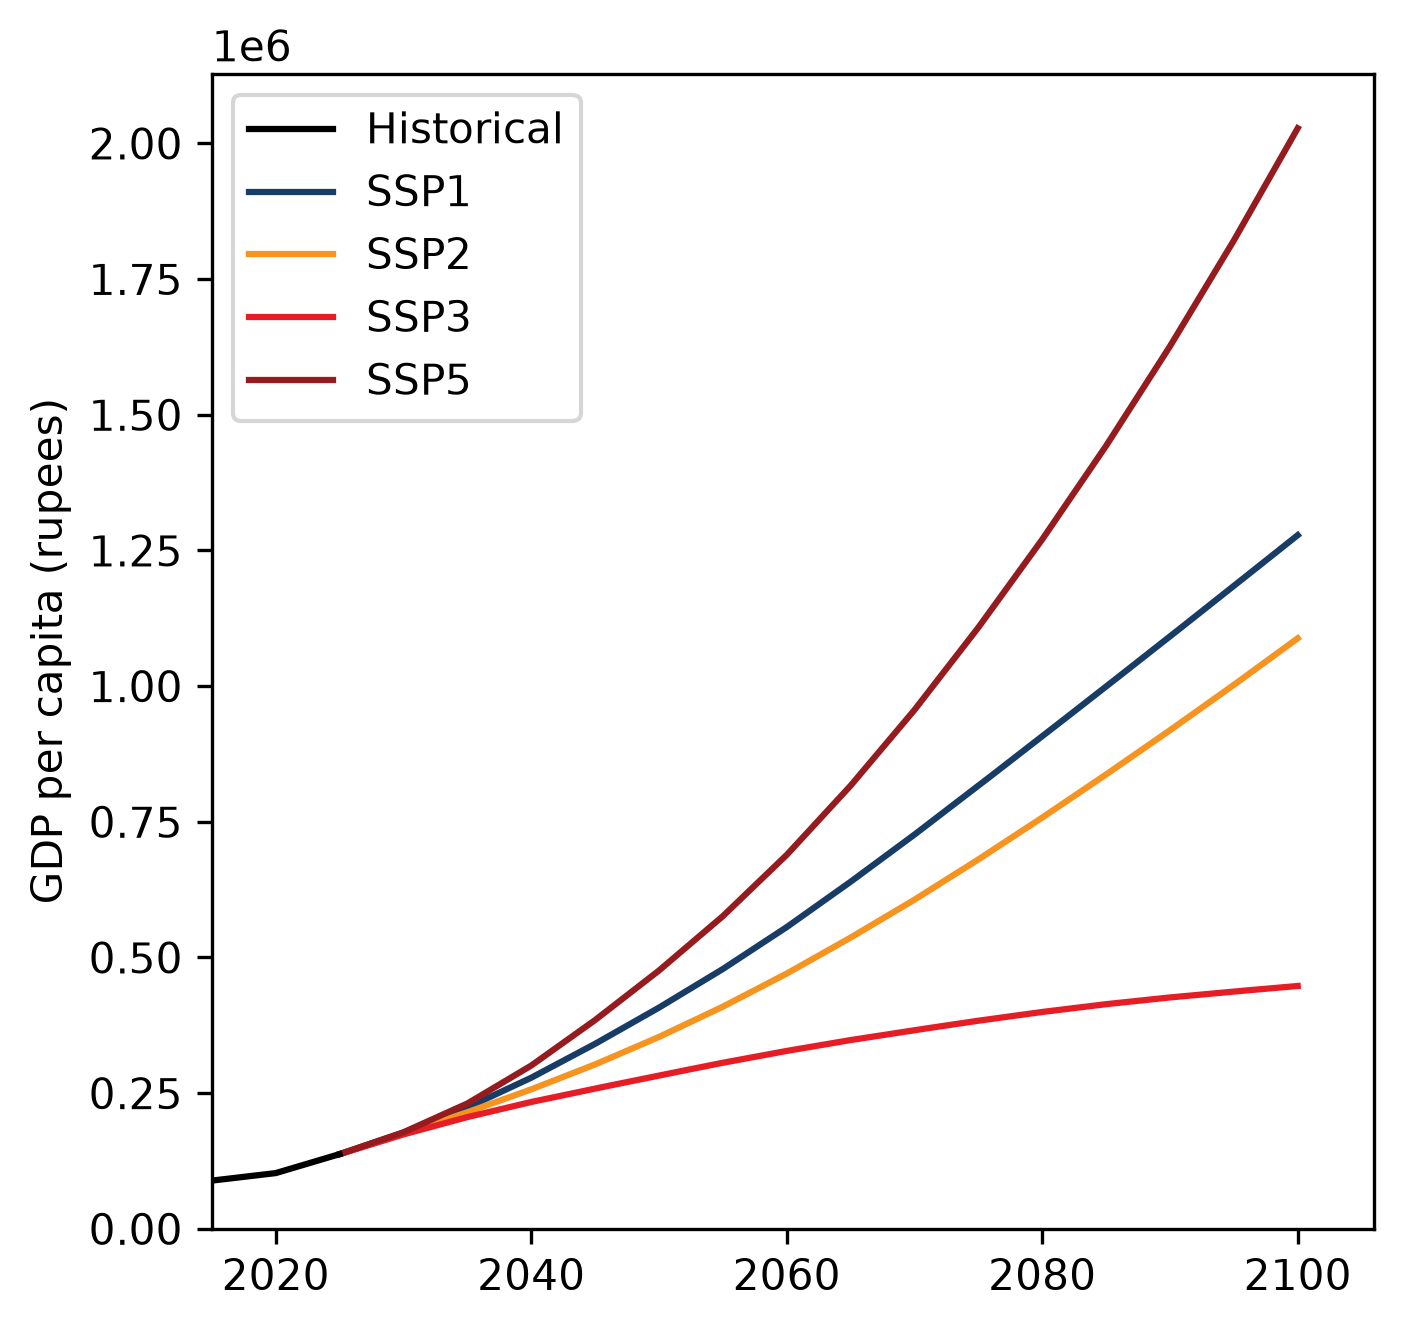
\includegraphics[width=0.49\columnwidth]{figures/projection_gdp_per_capita_india.png}
      \caption{\label{fig:proj_gdp_pop_india} Projections du nombre d'habitants et du PIB par habitant}
   \end{figure}

Ces projections nationales sont ensuite appliquées de manière homogène à l'ensemble des états indiens. Ainsi, en plus de l'hypothèse d'une distribution constante de la population dans le pays, on suppose que l'évolution du PIB par habitant suit la même logique. Pour ensuite avoir le nombre de logements (pour le calcul du nombre de systèmes de climatisation par état), on suppose un nombre constant de personnes par logement, différent selon les états et calculé d'après les données d'enquête de 2023. En moyenne cette valeur vaut \num{4.76}. 

\section{Projections de taux d'équipement et nombre de systèmes de climatisation}

En appliquant les projections de CDD26 et de PIB par habitant (avec une moyenne mobile de période \SI{10}{\ans}) à l'expression décrite \eqref{eq:es}, on obtient les projections de taux d'équipement de climatisation par logement et par état pour chaque scénario et modèle climatique. En multipliant ce taux par le nombre de logements et le nombre moyen de systèmes de climatisation par ménage équipé -- \num{1.23} (\cite{mspi_nss_2023}) -- on obtient des projections de nombres de systèmes. La \ref{fig:proj_ac_india} illustre ces résultats à l'échelle de l'Inde. Les résultats par état sont décrits en annexe (\ref{sec:projections_par_etat}) et disponibles dans le fichier \texttt{data/AC\_projection.csv} du dépôt git.

   \begin{figure}[ht]
      \centering
      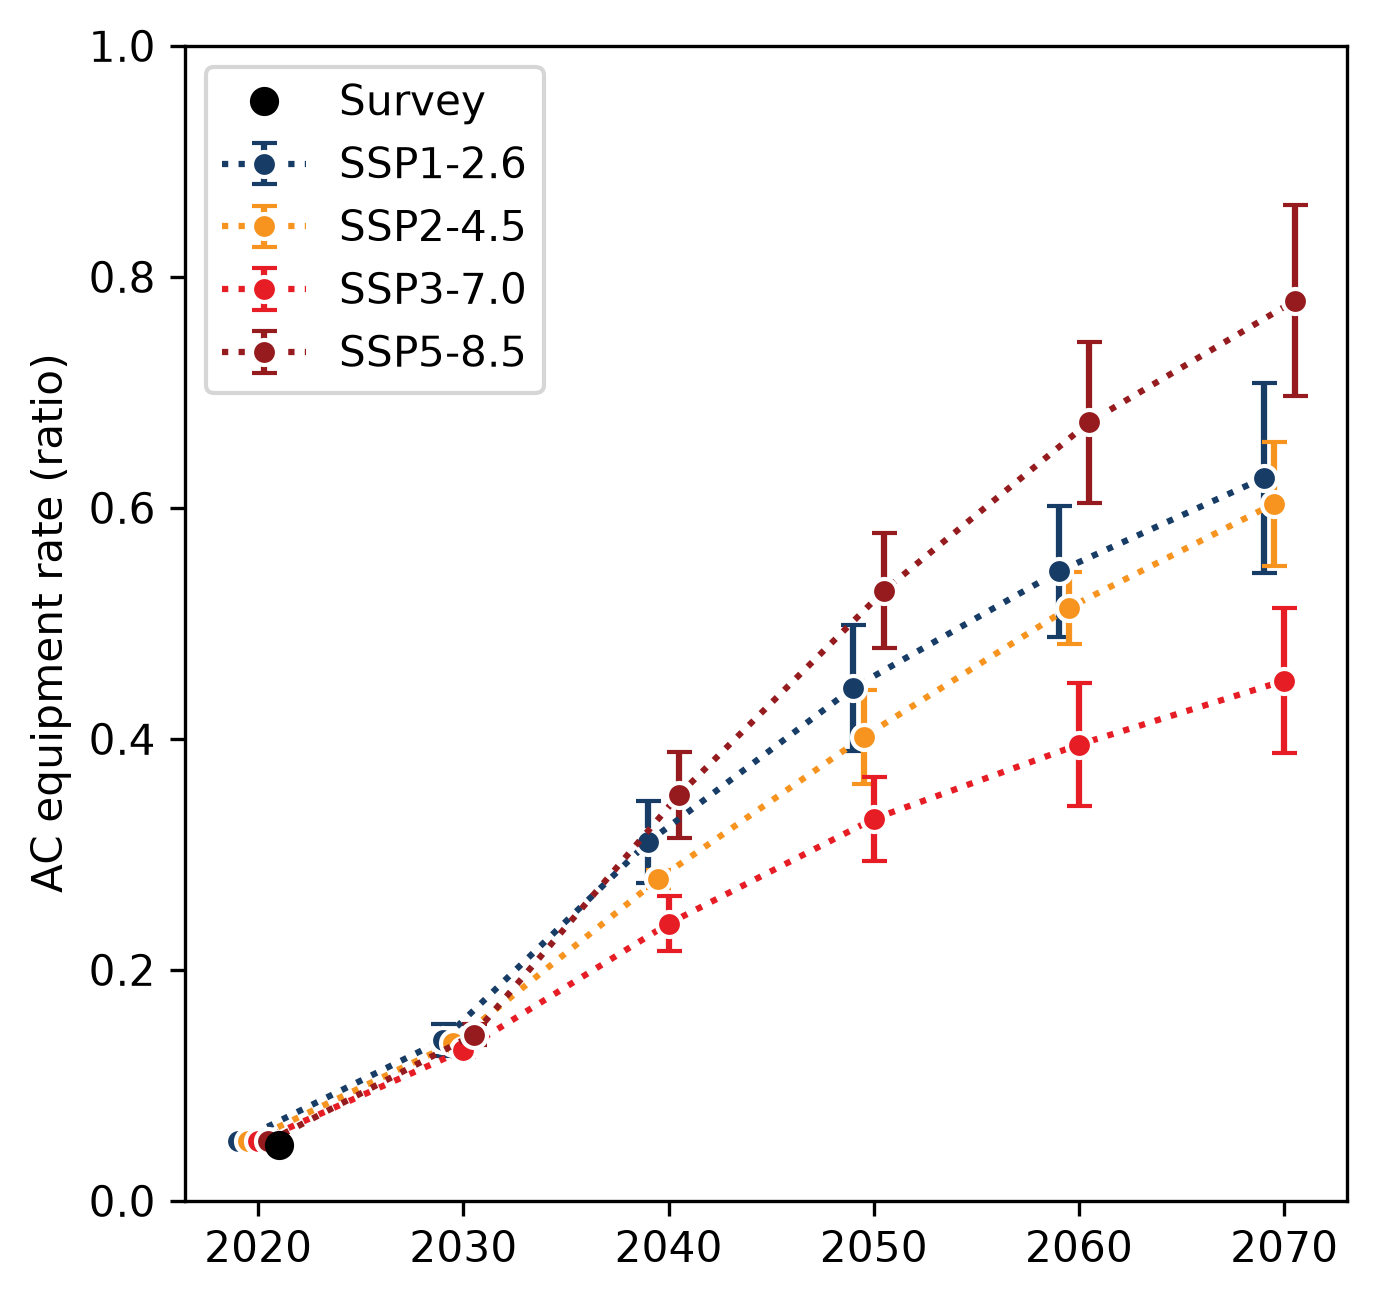
\includegraphics[width=0.49\columnwidth]{figures/projection_ac_rate_india.png}
      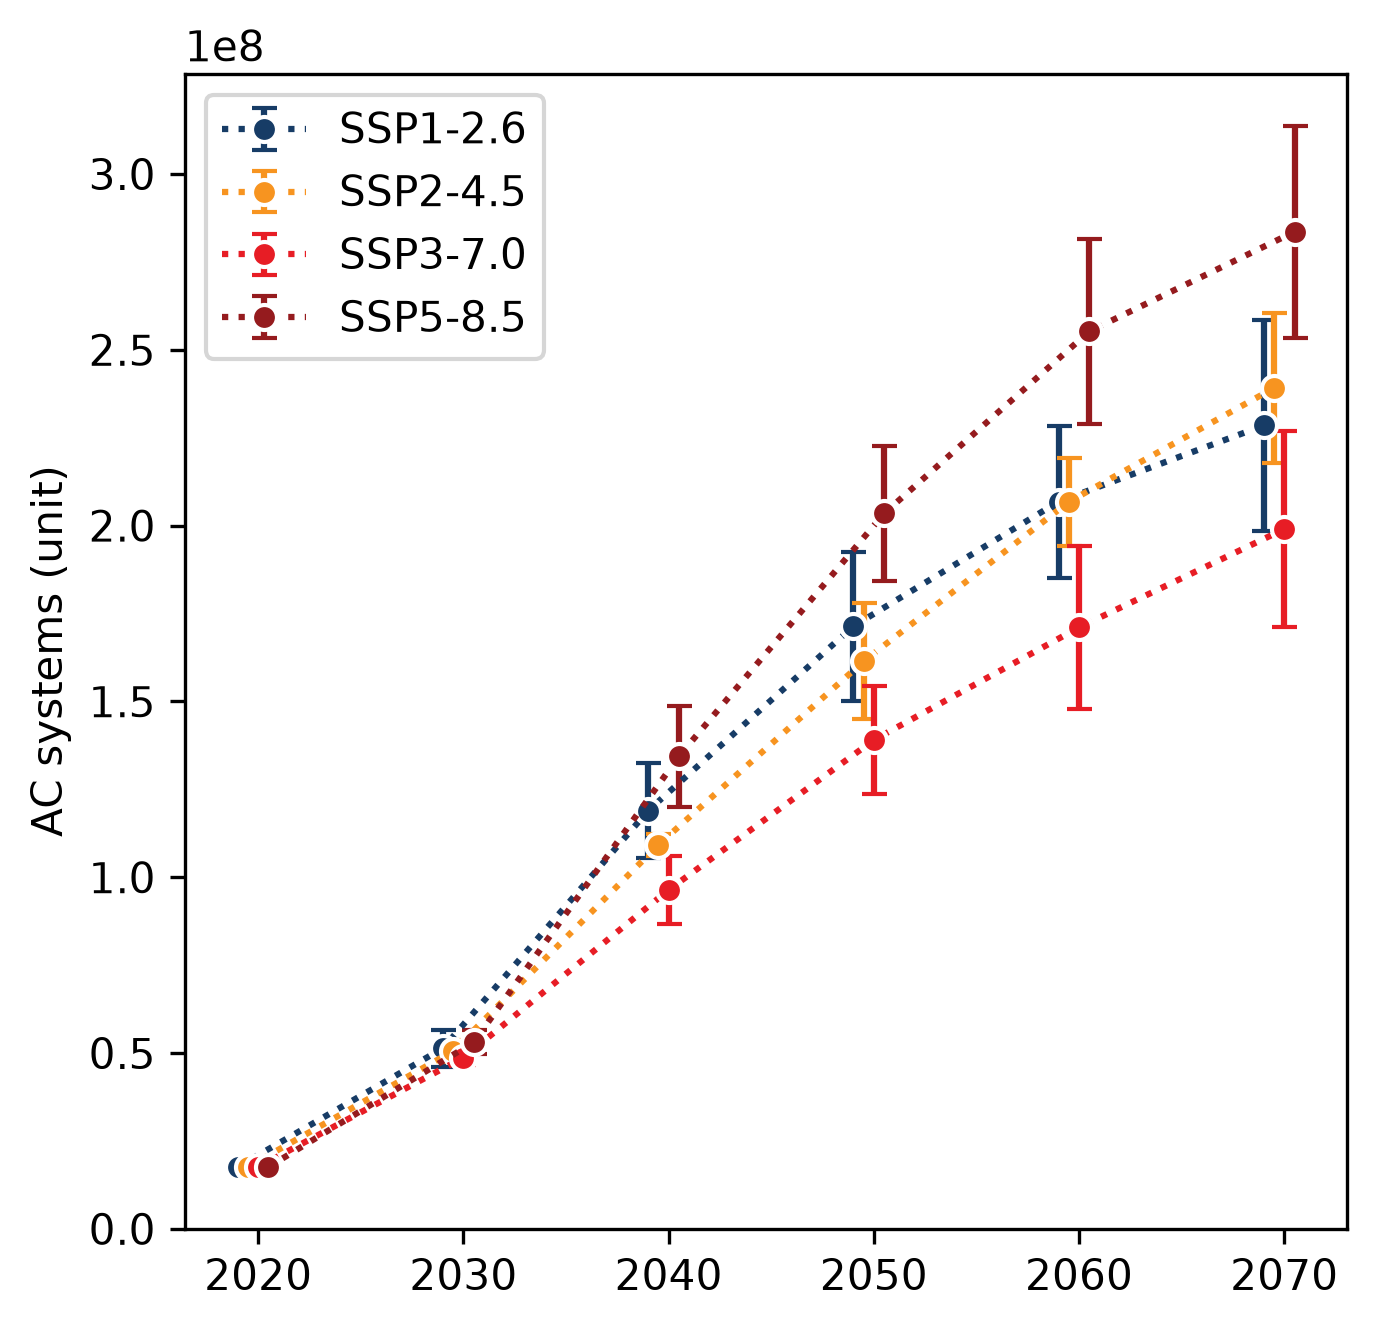
\includegraphics[width=0.49\columnwidth]{figures/projection_ac_systems_india.png}
      \caption{\label{fig:proj_ac_india} Projections du taux d'équipement en climatisation et du nombre de systèmes}
   \end{figure}

\clearpage
\appendix 

\section{Annexes}

\subsection{Projections par état} \label{sec:projections_par_etat}

Certains petits états (Daman and Diu, Andaman and Nicobar, Lakshadweep, Ladakh, Dadra and Nagar Haveli, Arunachal Pradesh, Chandigarh, Jammu and Kashmir) ne sont pas disponibles dans les données climatologiques ou de population et sont exclus de l'analyse. 

\subsubsection{Andhra Pradesh}

\begin{figure}[ht]
   \centering
   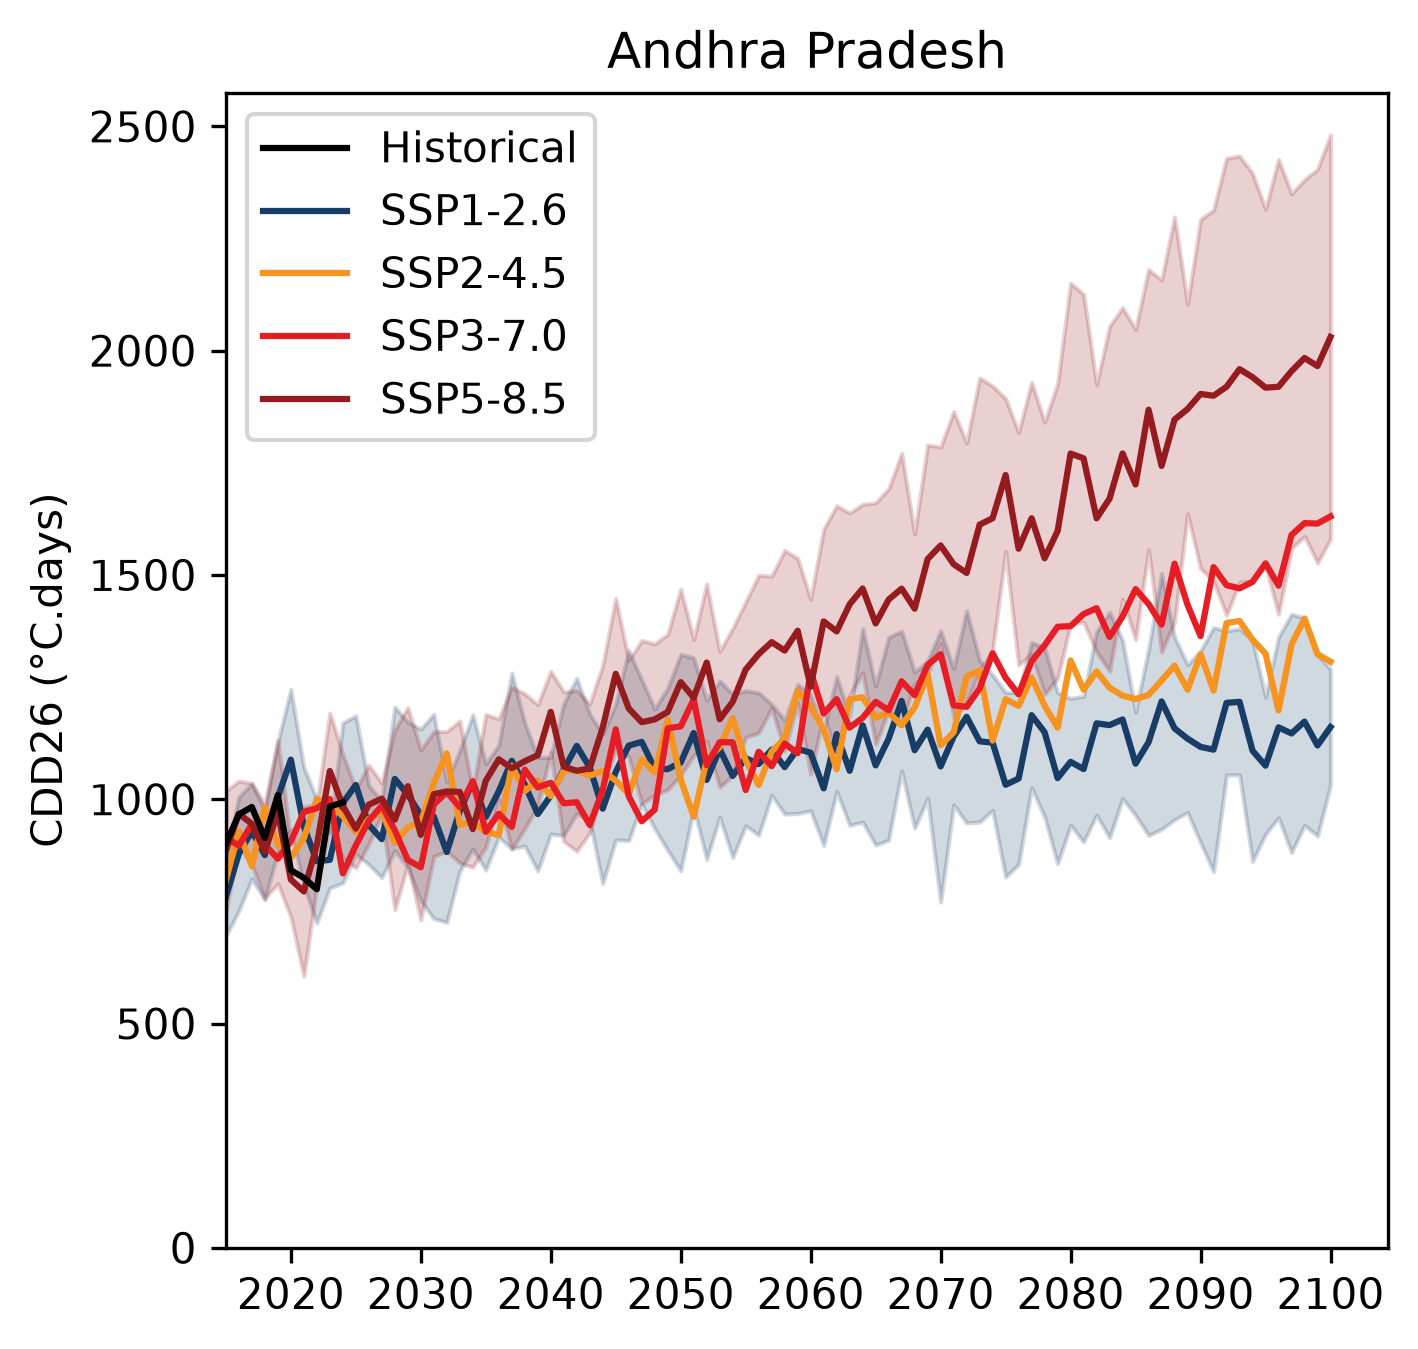
\includegraphics[height=0.25\textheight]{figures/projection_states/projection_cdd26_Andhra Pradesh.png}\hfill
   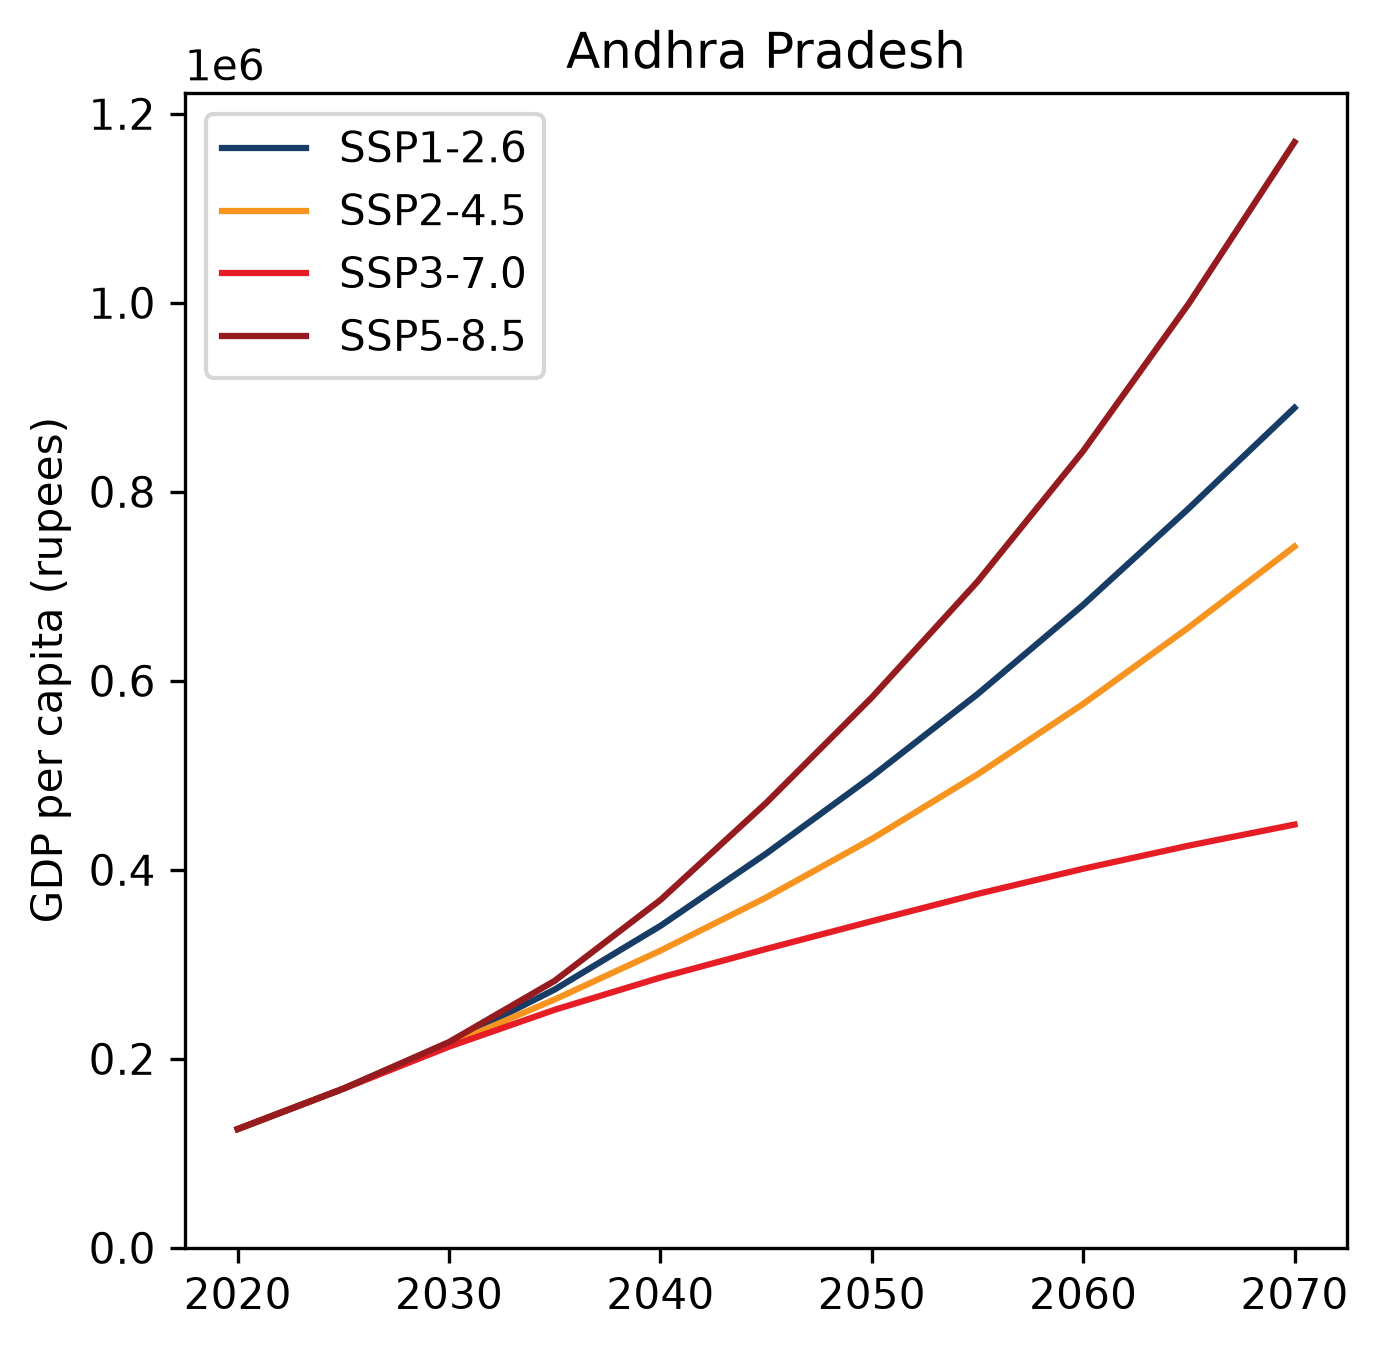
\includegraphics[height=0.25\textheight]{figures/projection_states/projection_gdp_per_capita_Andhra Pradesh.png}\\
   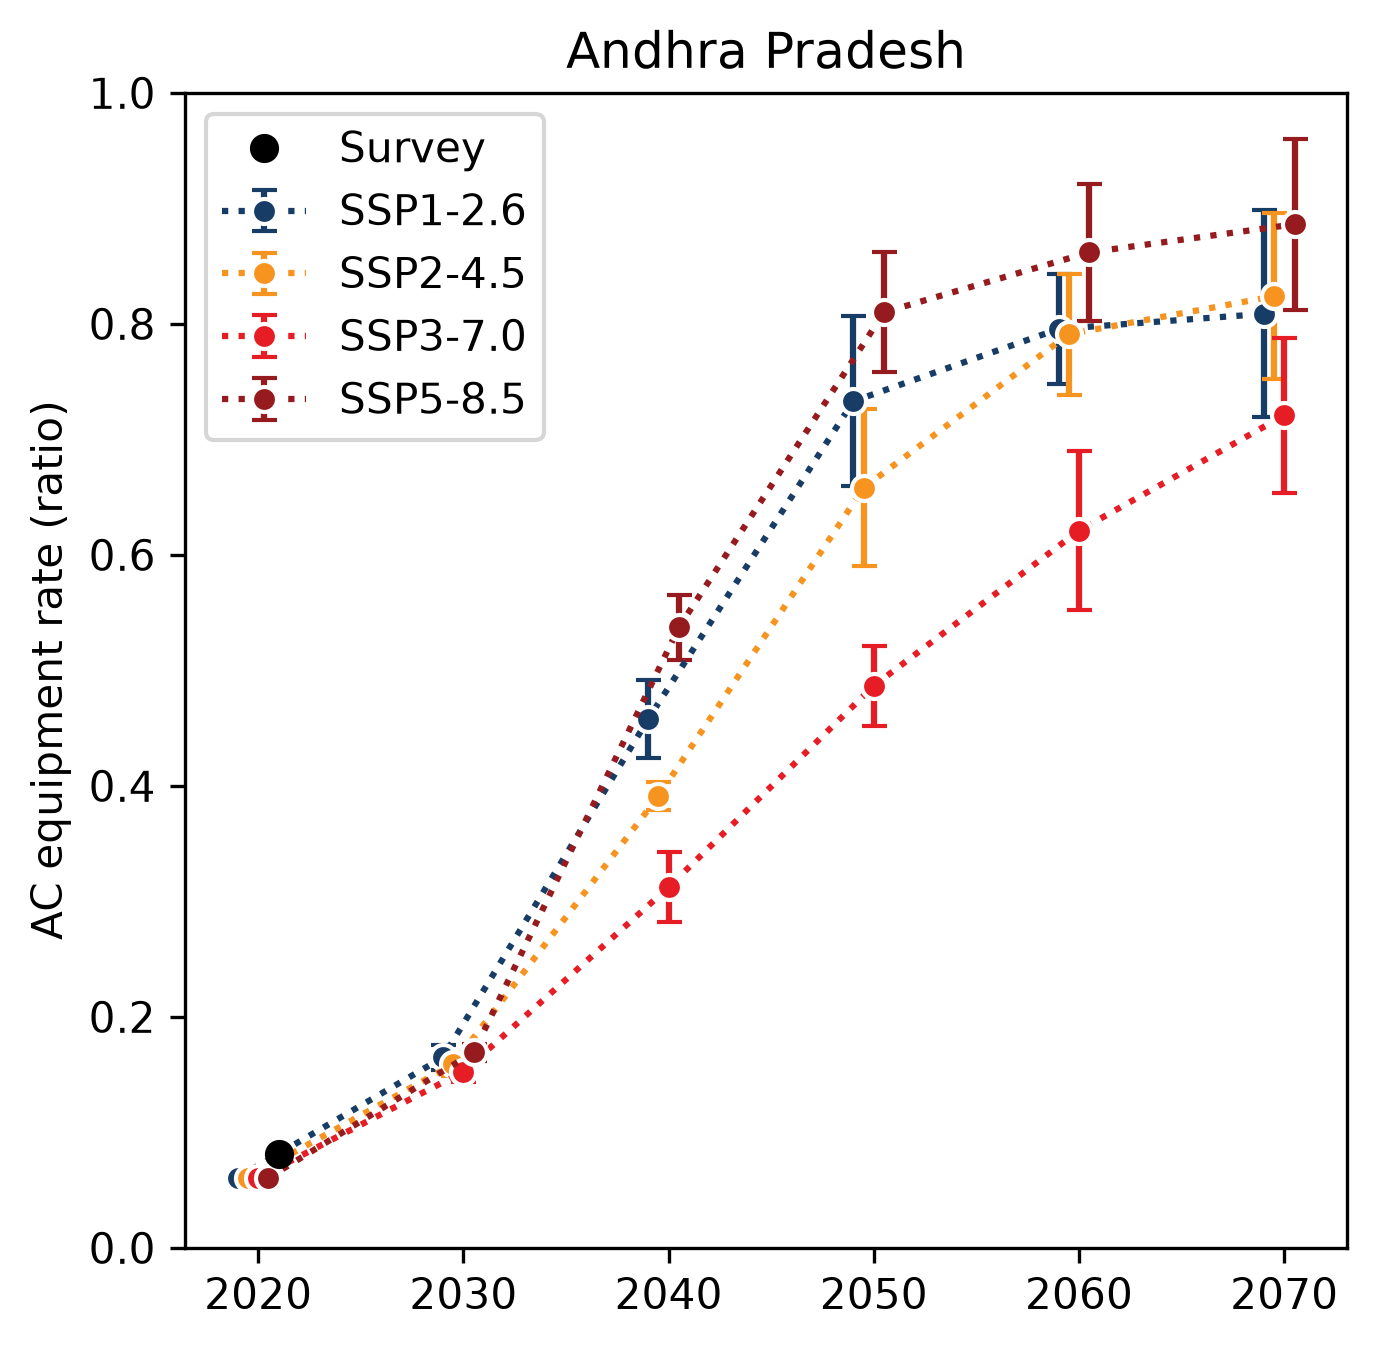
\includegraphics[height=0.25\textheight]{figures/projection_states/projection_ac_rate_Andhra Pradesh.png}\hfill
   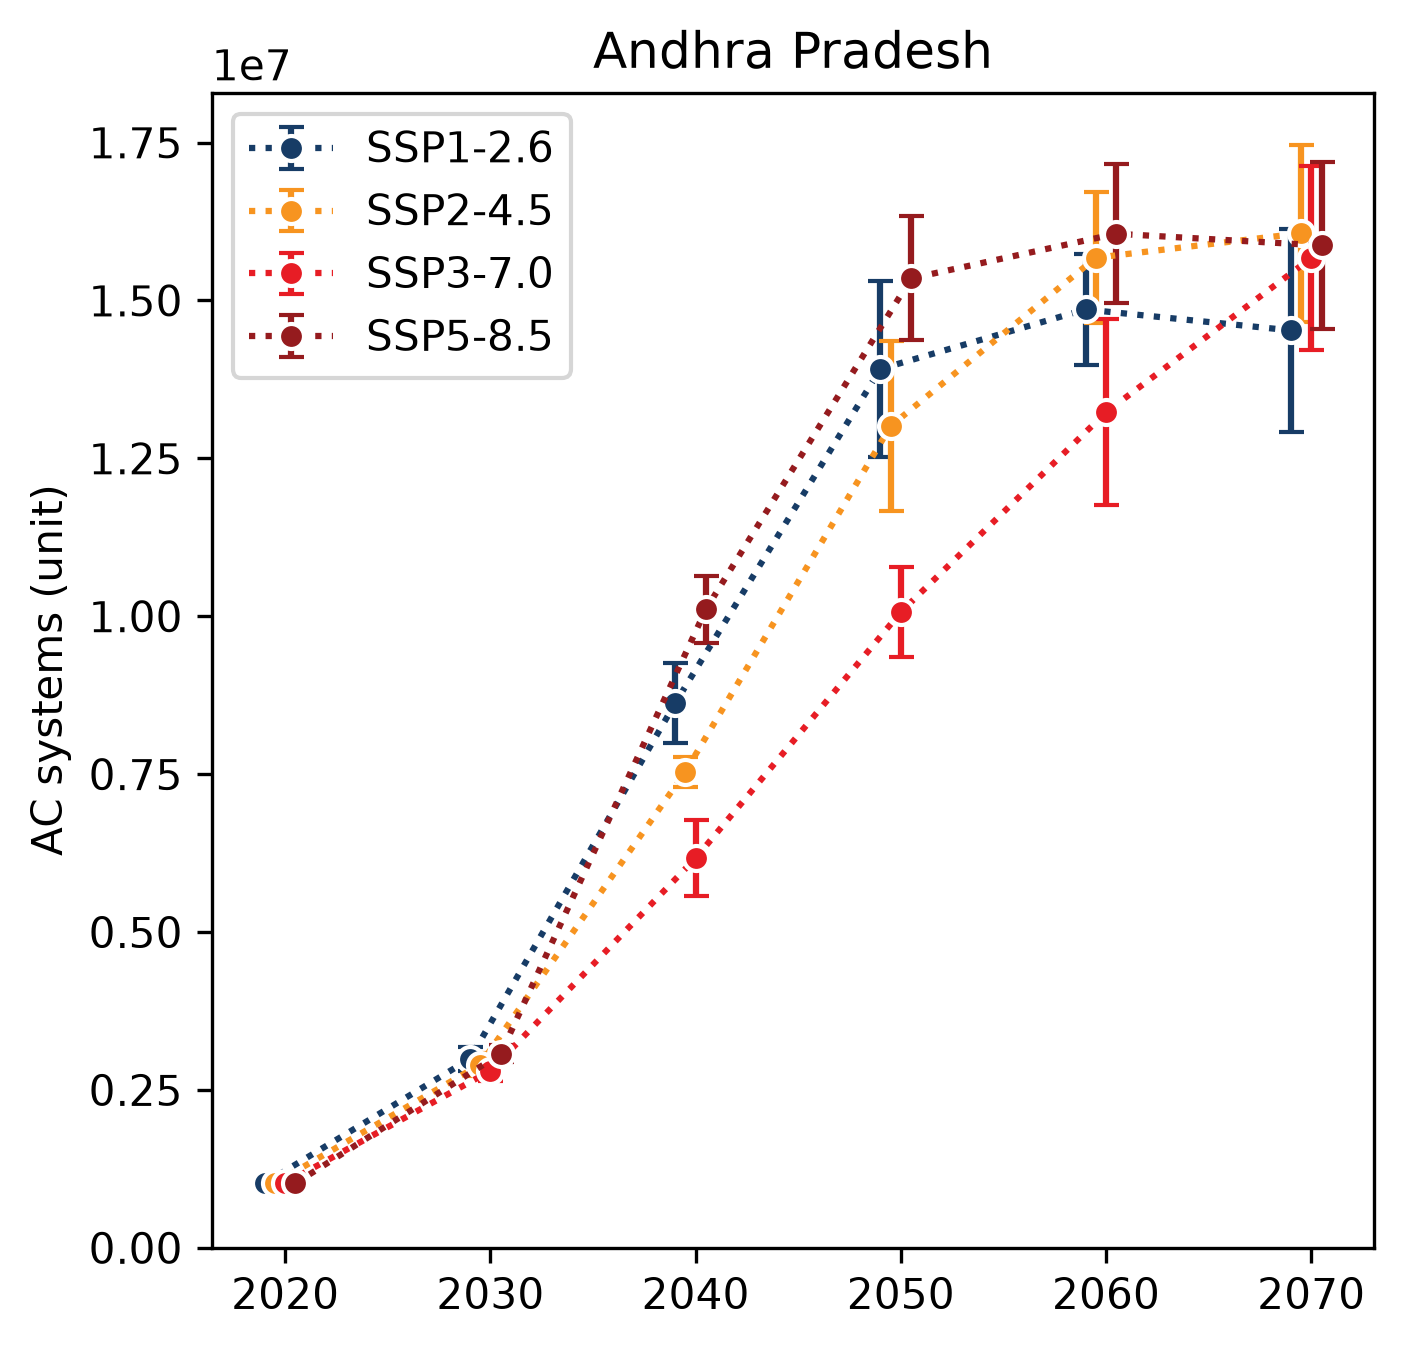
\includegraphics[height=0.25\textheight]{figures/projection_states/projection_ac_systems_Andhra Pradesh.png}
   \caption{Projections des différentes variables pour Andhra Pradesh}
\end{figure}

\clearpage

\subsubsection{Assam}

\begin{figure}[ht]
   \centering
   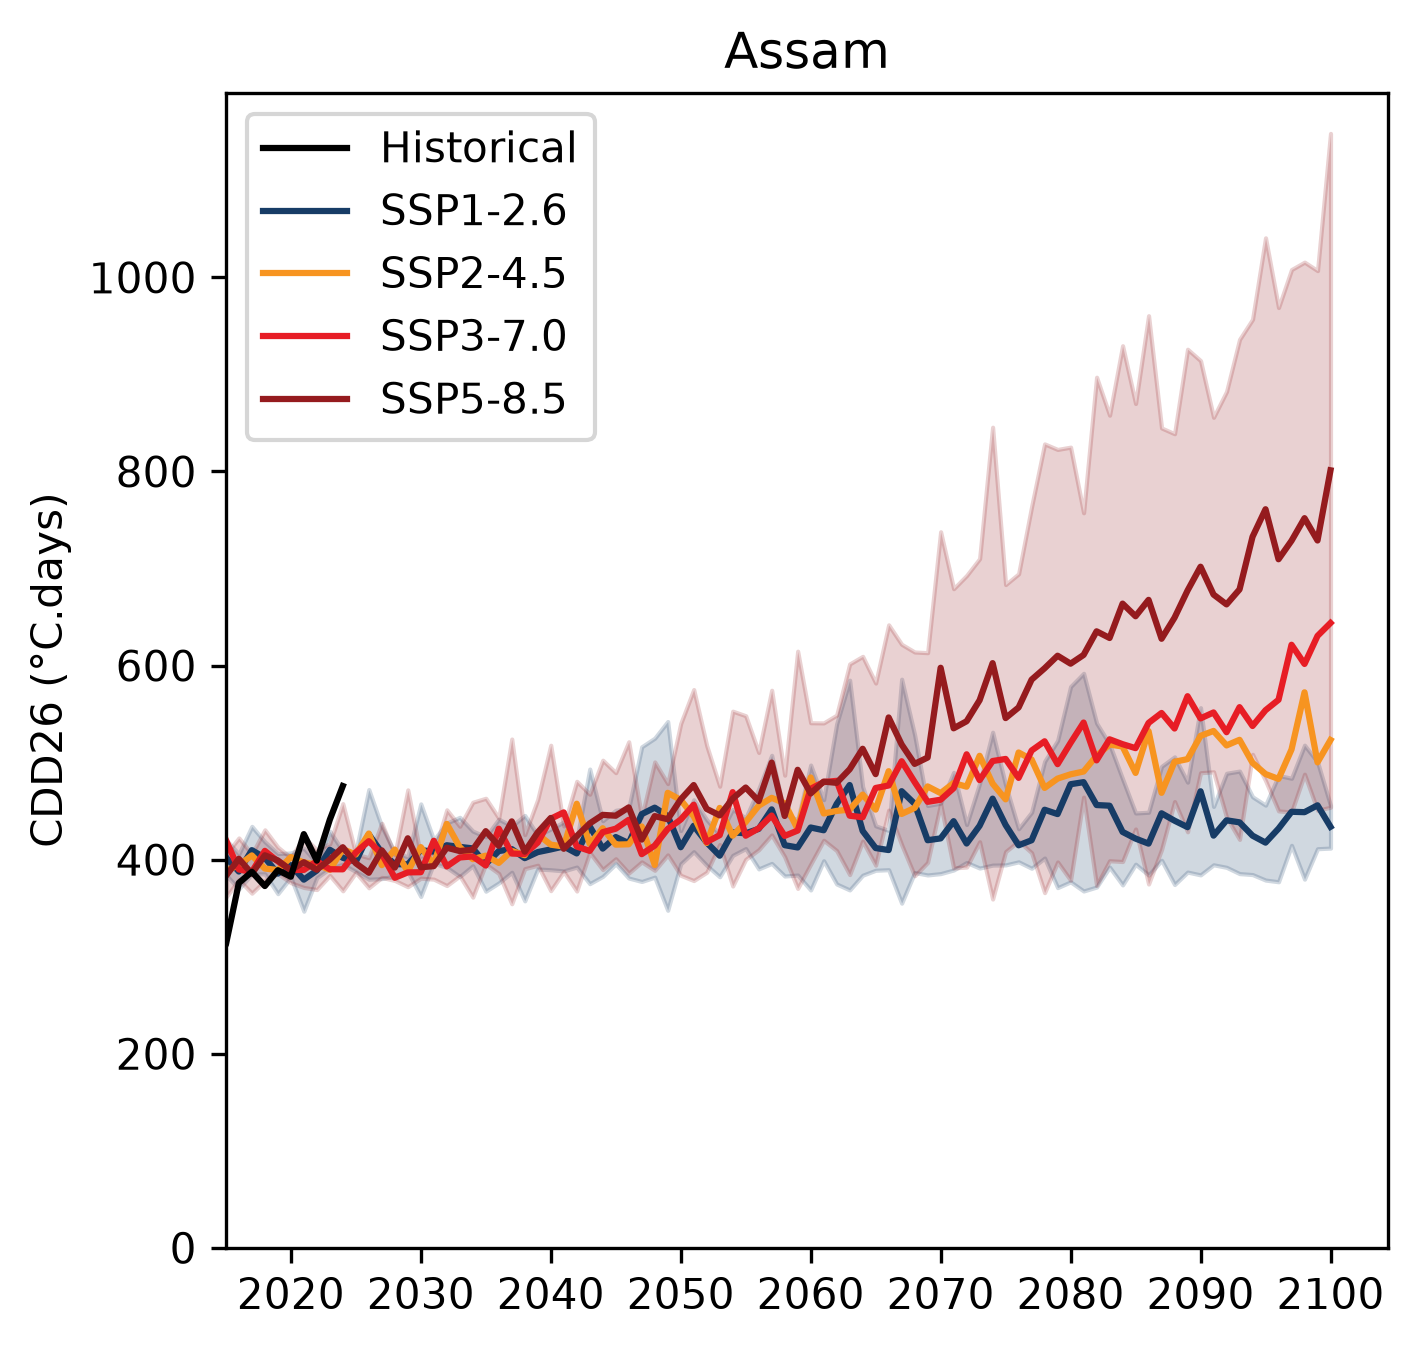
\includegraphics[height=0.25\textheight]{figures/projection_states/projection_cdd26_Assam.png}\hfill
   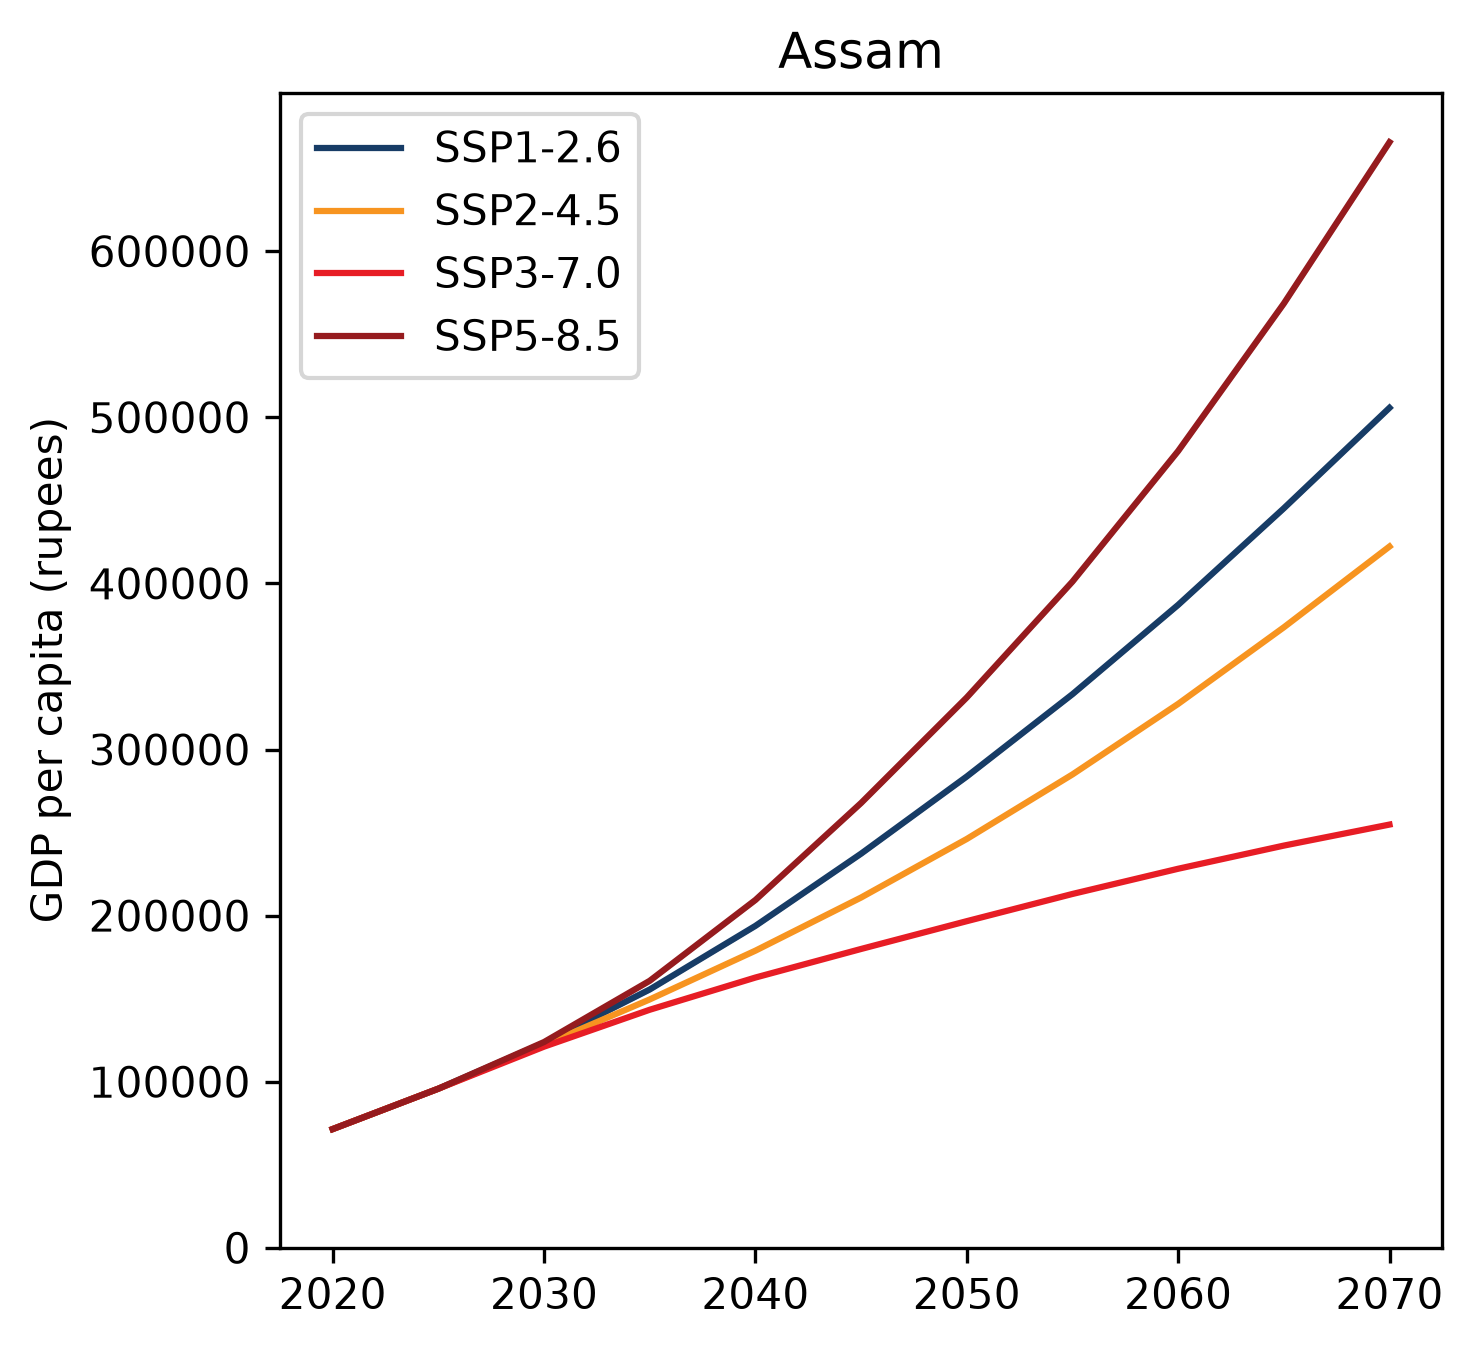
\includegraphics[height=0.25\textheight]{figures/projection_states/projection_gdp_per_capita_Assam.png}\\
   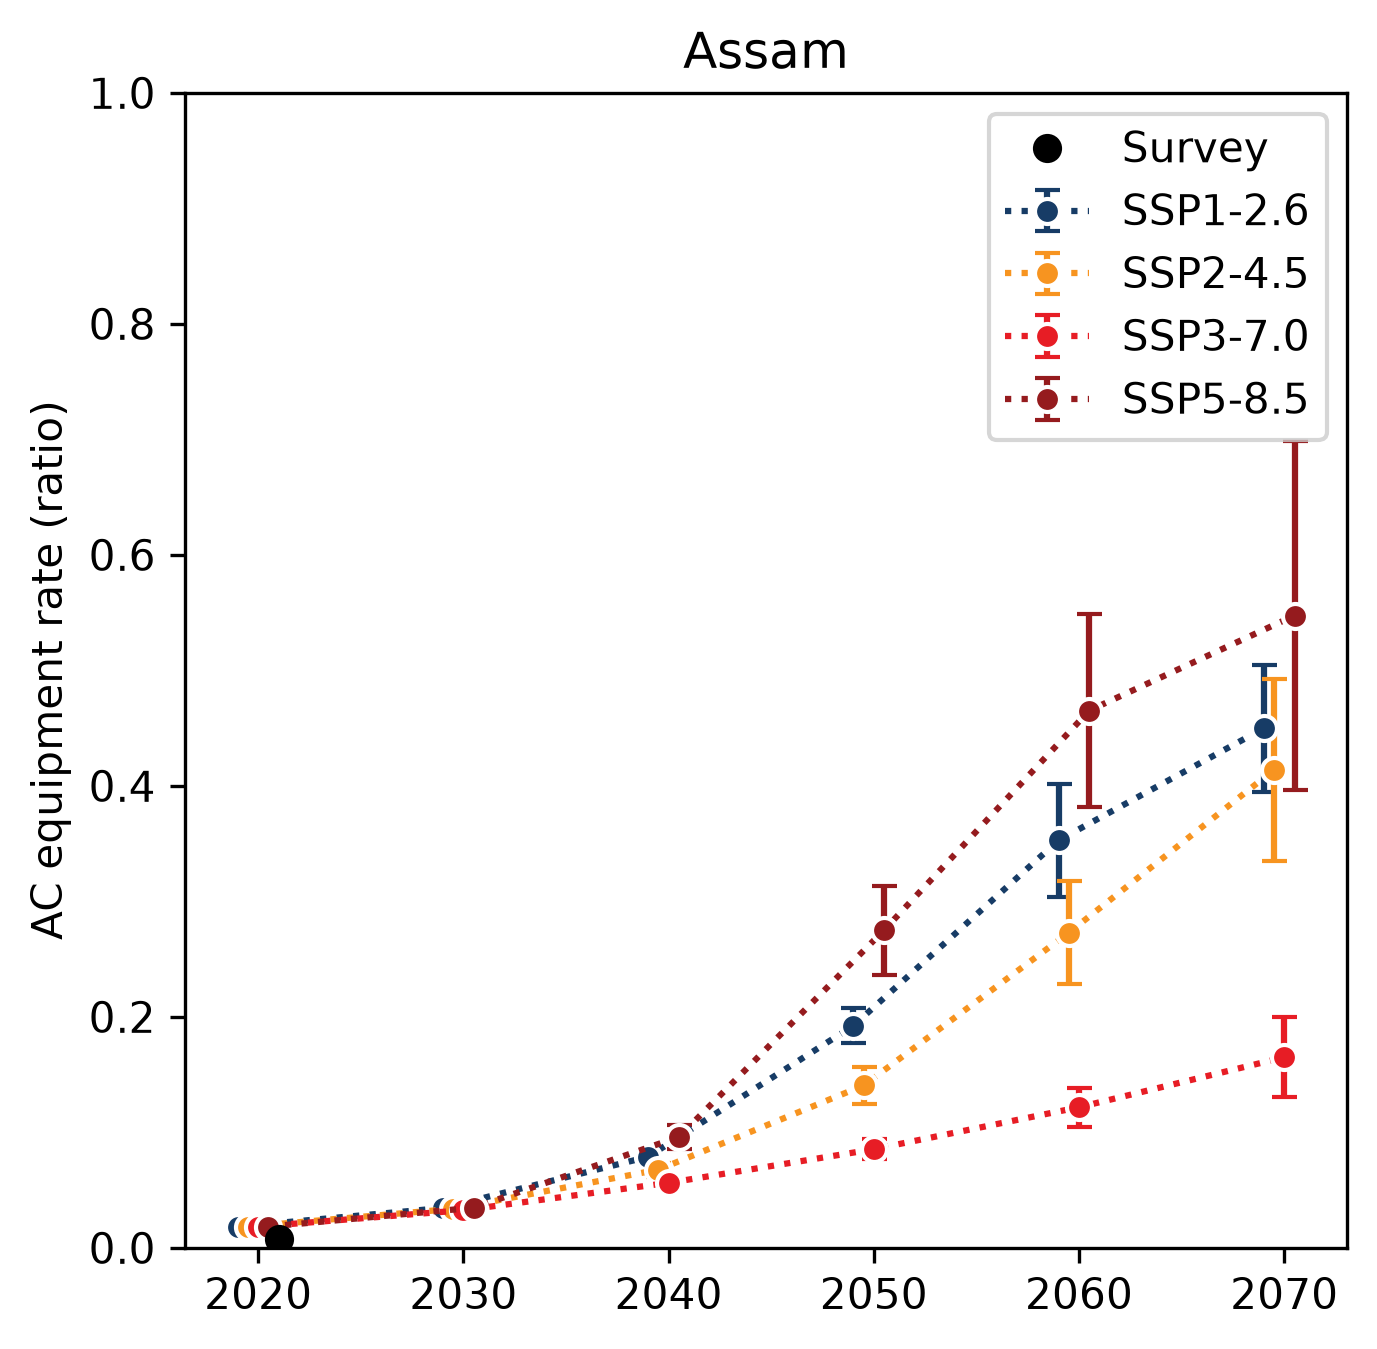
\includegraphics[height=0.25\textheight]{figures/projection_states/projection_ac_rate_Assam.png}\hfill
   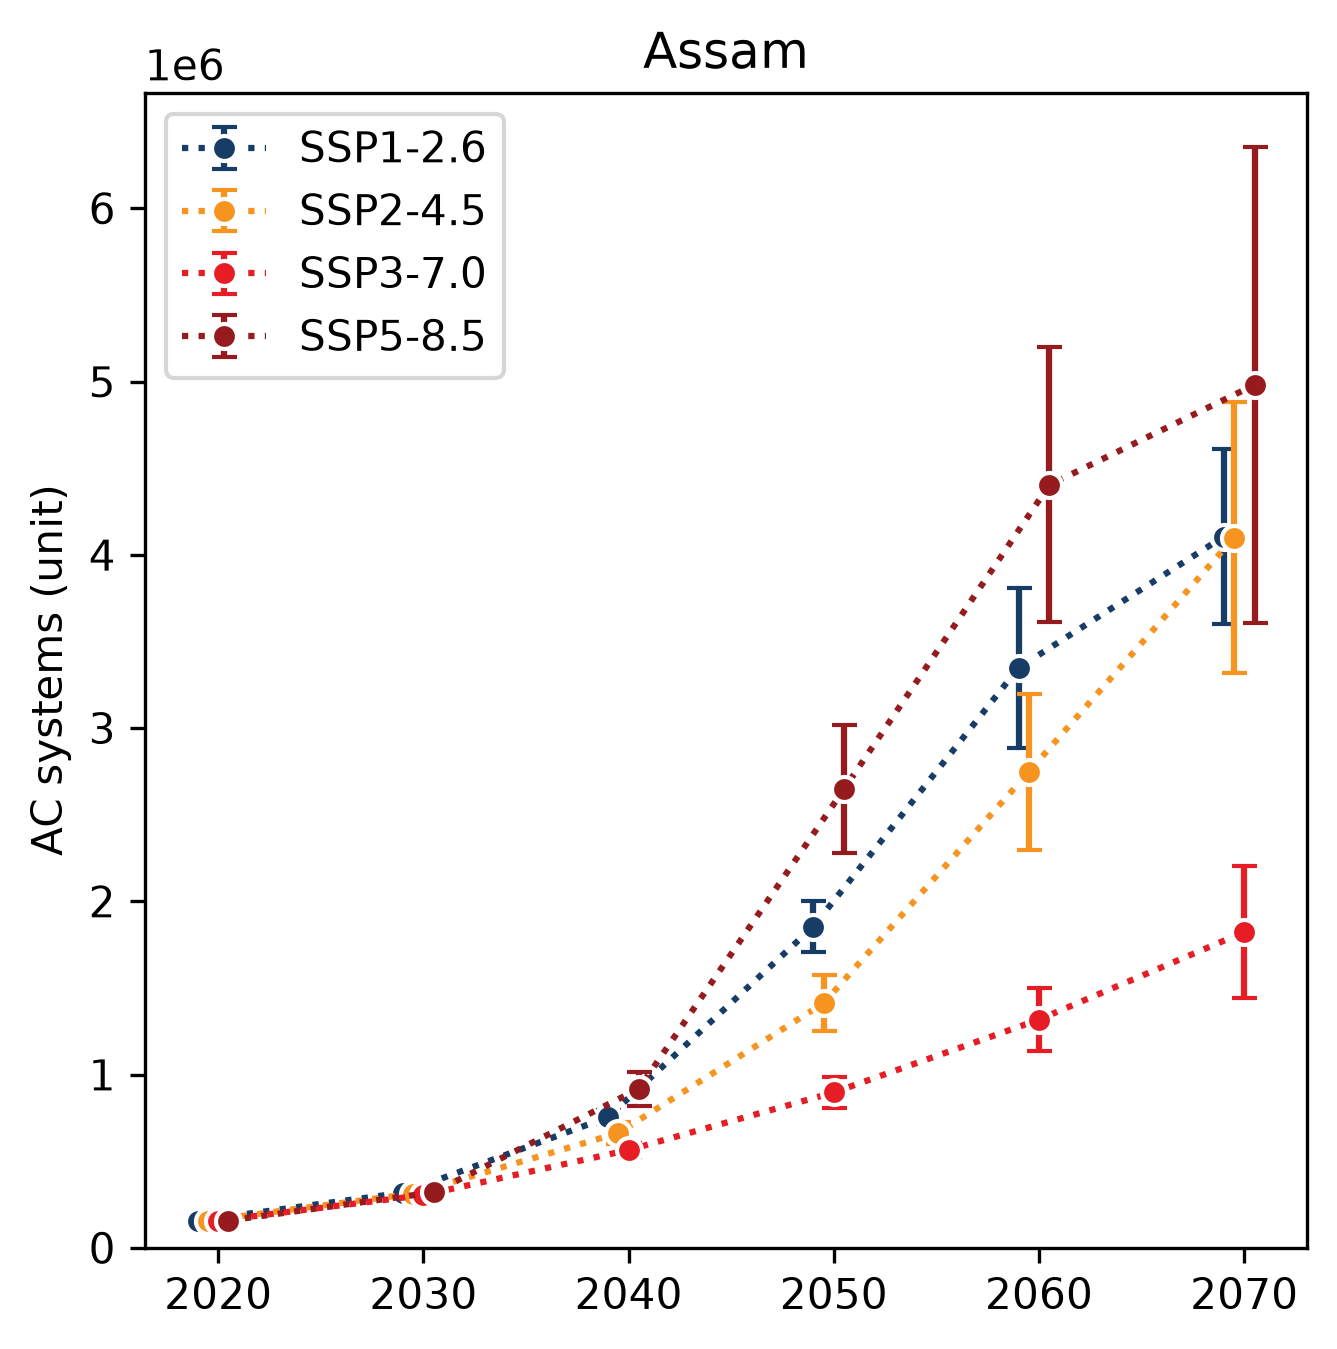
\includegraphics[height=0.25\textheight]{figures/projection_states/projection_ac_systems_Assam.png}
   \caption{Projections des différentes variables pour Assam}
\end{figure}

\clearpage

\subsubsection{Bihar}

\begin{figure}[ht]
   \centering
   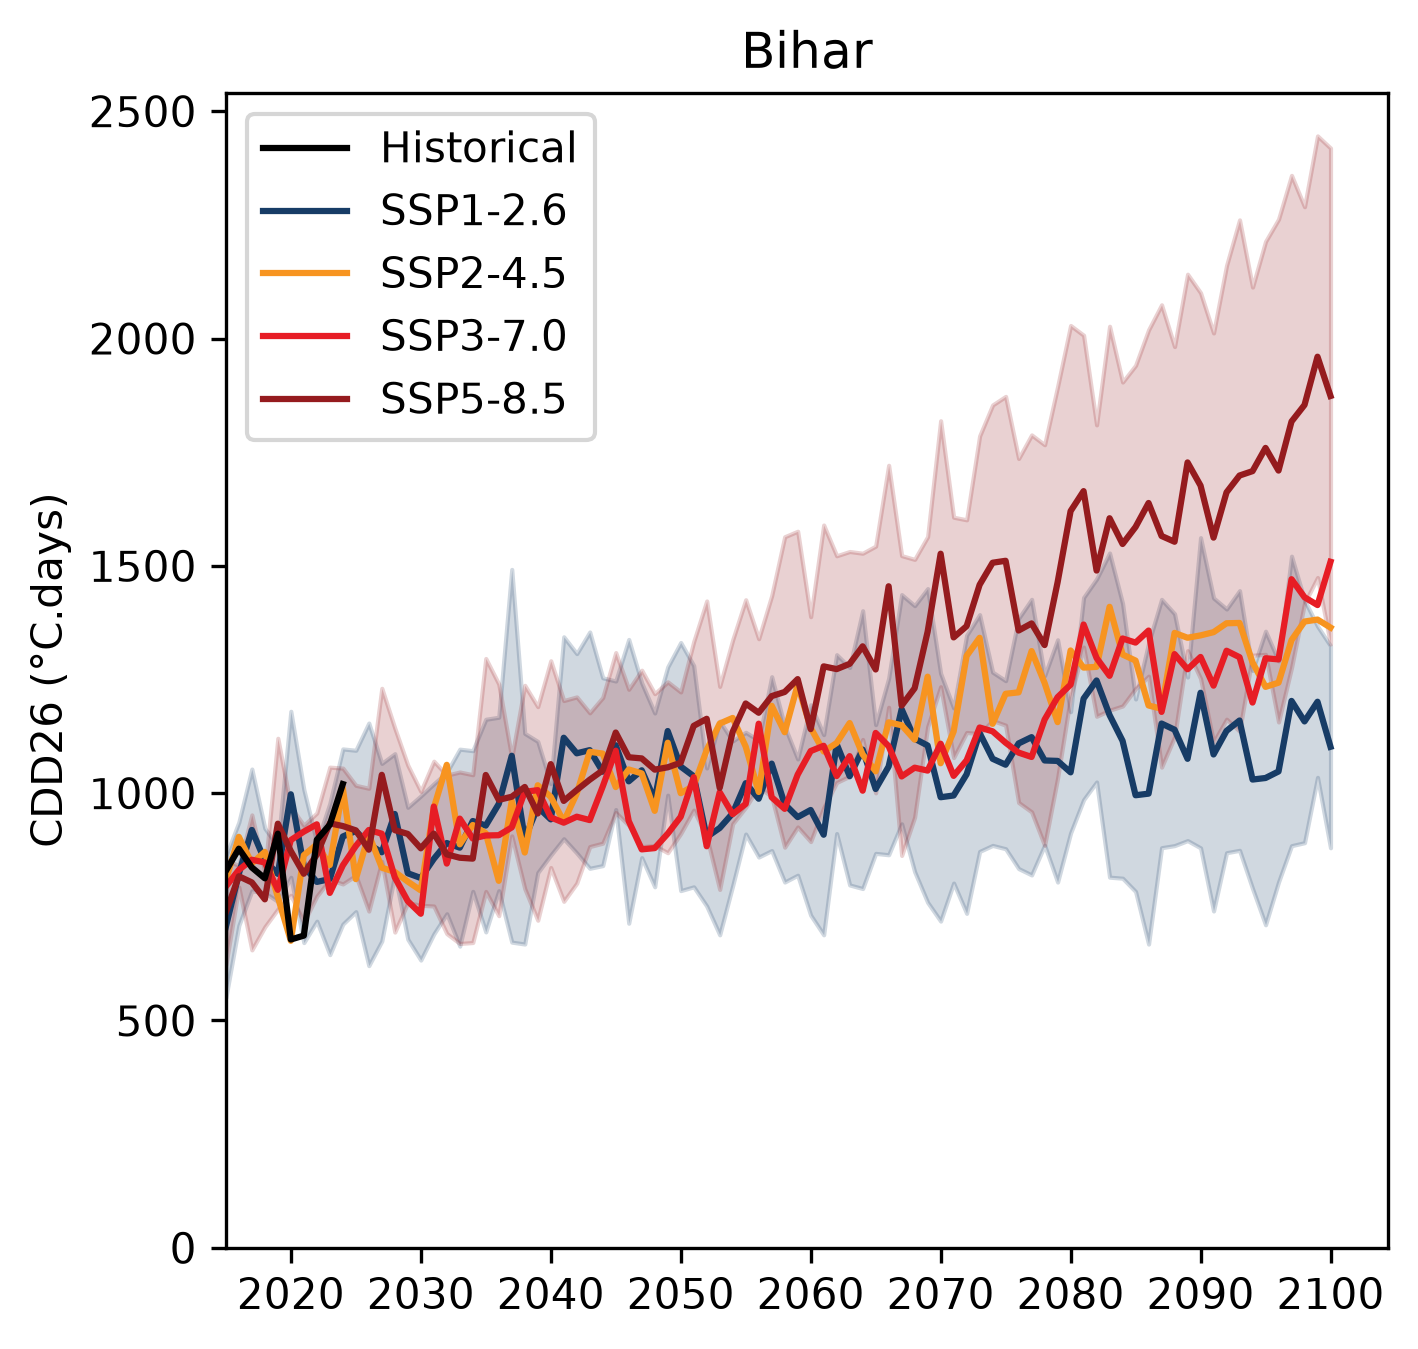
\includegraphics[height=0.25\textheight]{figures/projection_states/projection_cdd26_Bihar.png}\hfill
   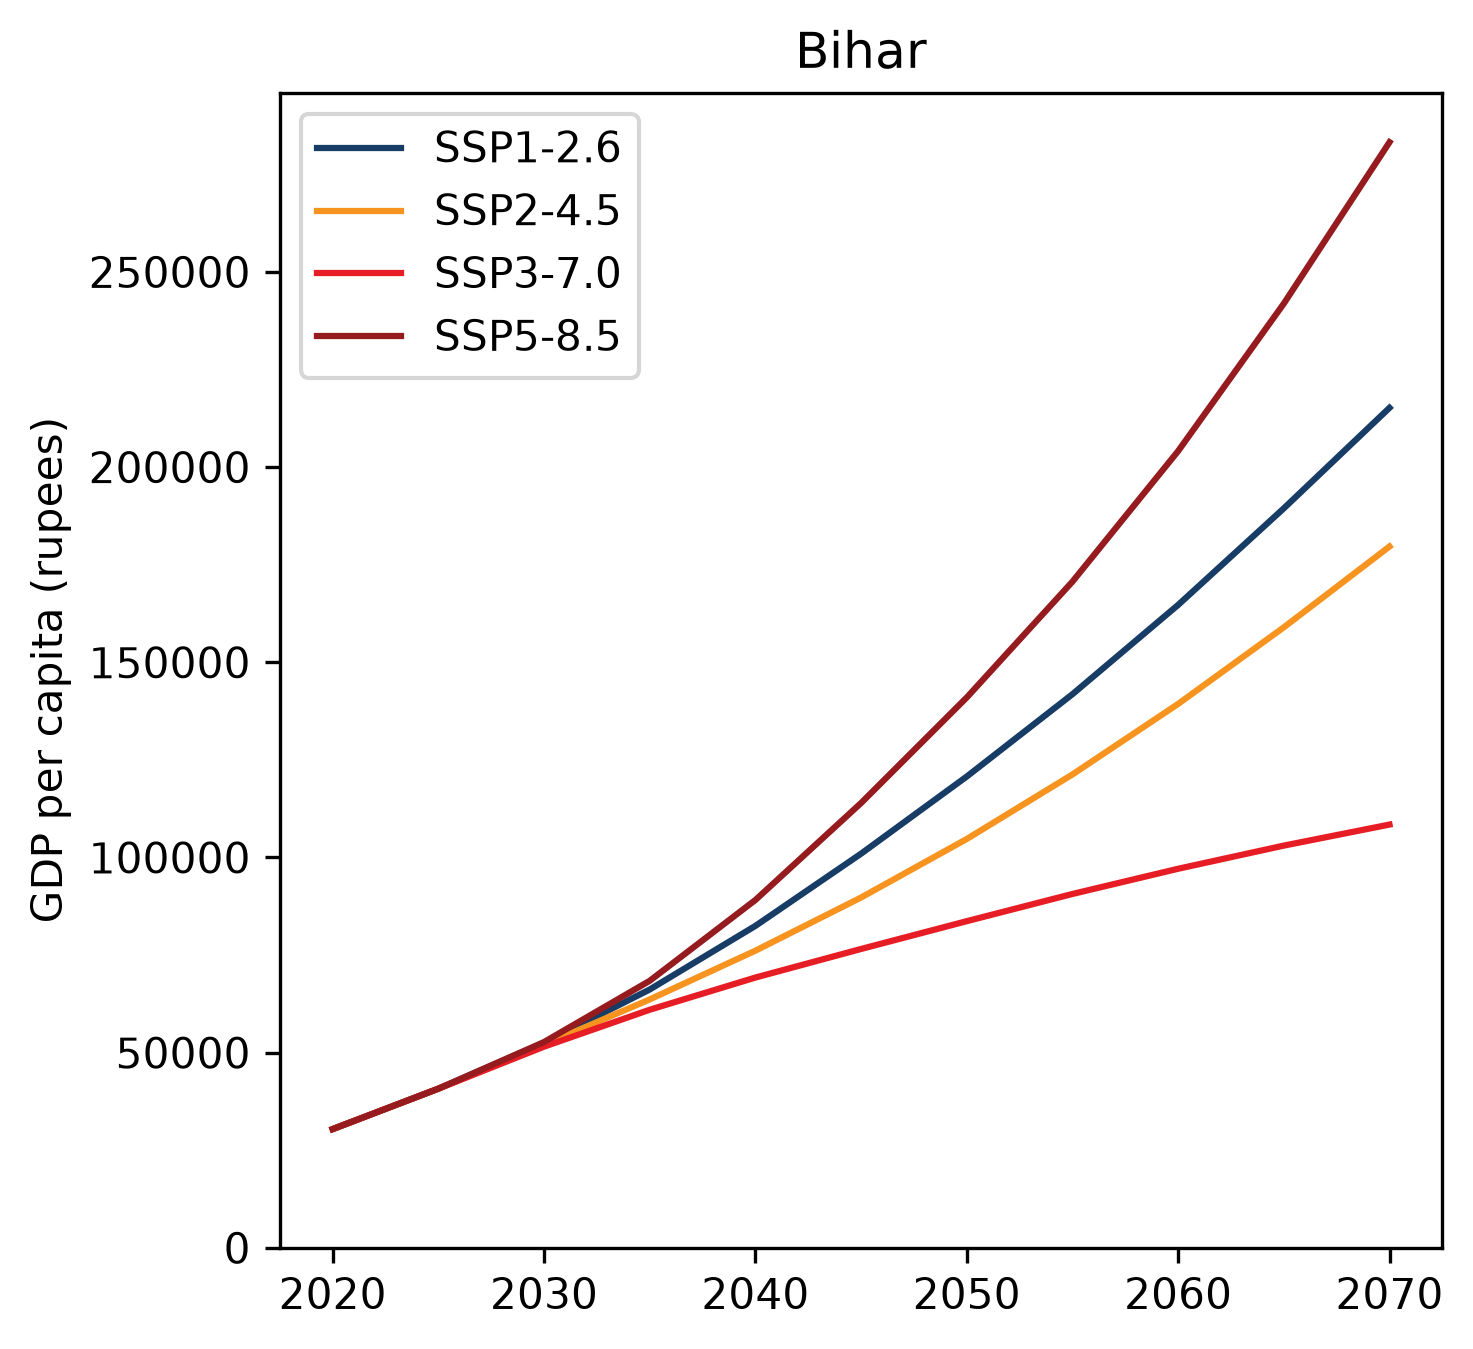
\includegraphics[height=0.25\textheight]{figures/projection_states/projection_gdp_per_capita_Bihar.png}\\
   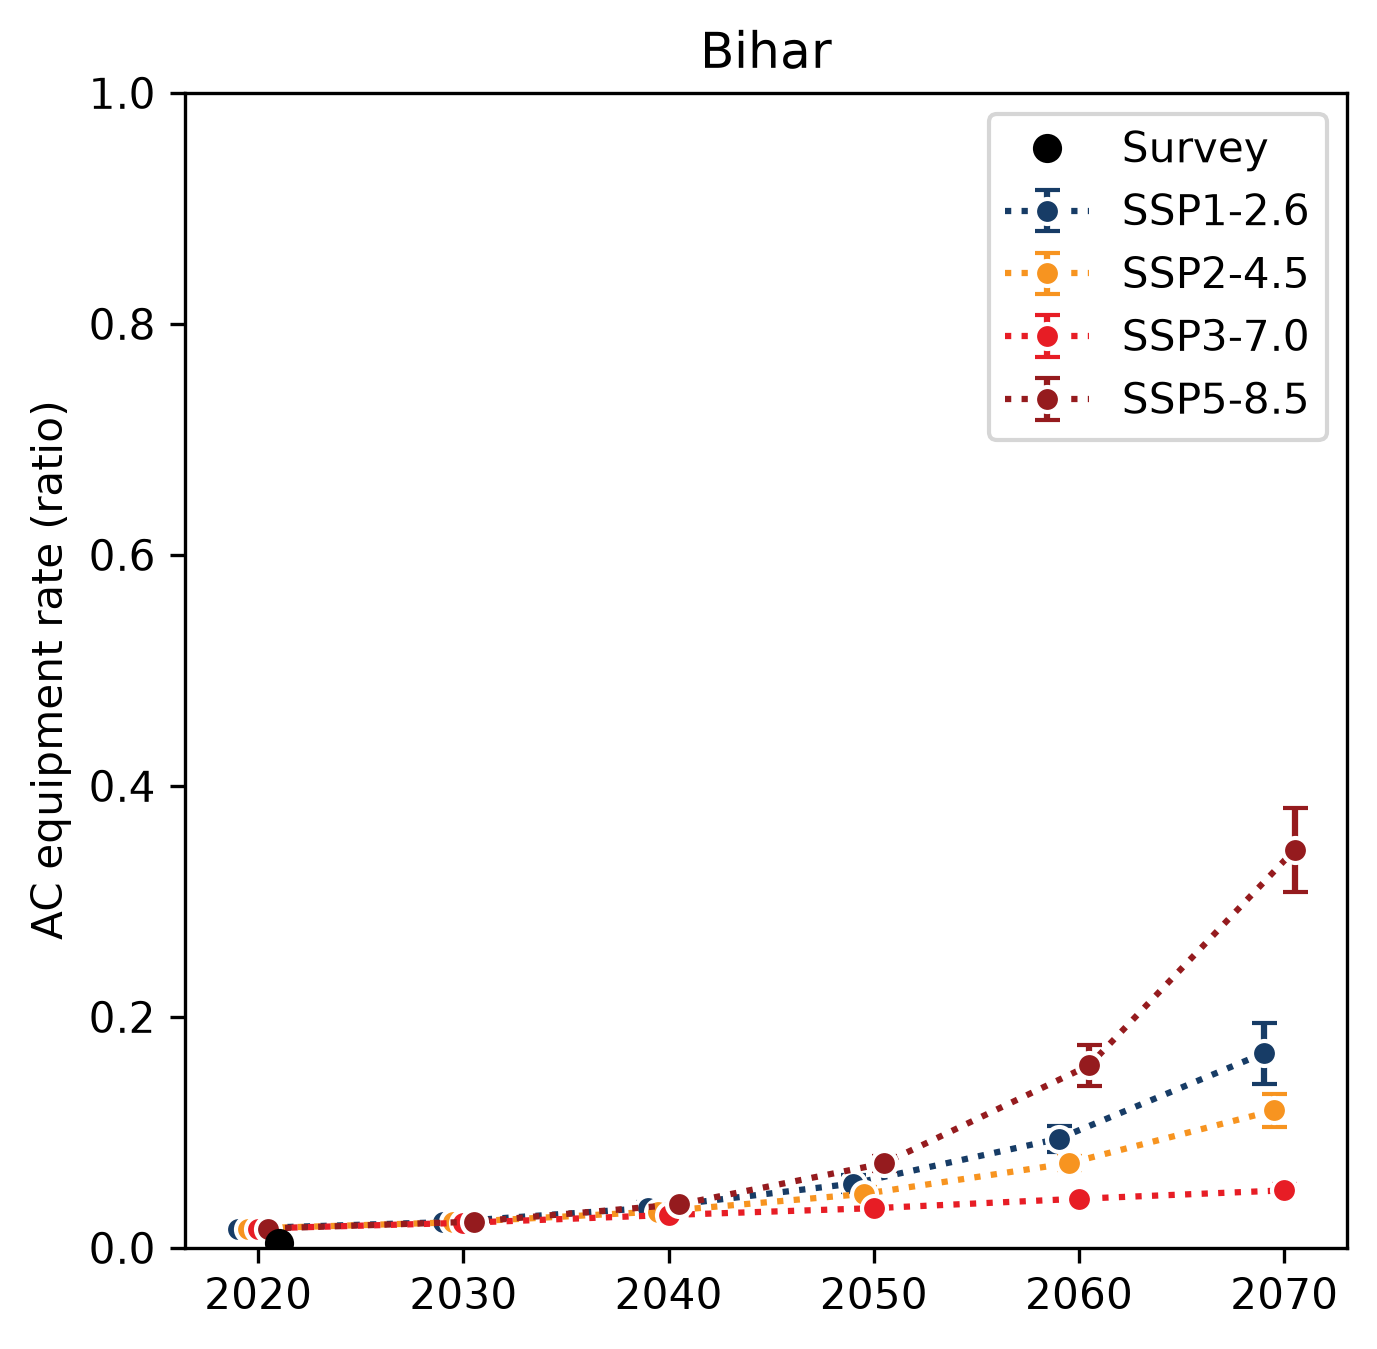
\includegraphics[height=0.25\textheight]{figures/projection_states/projection_ac_rate_Bihar.png}\hfill
   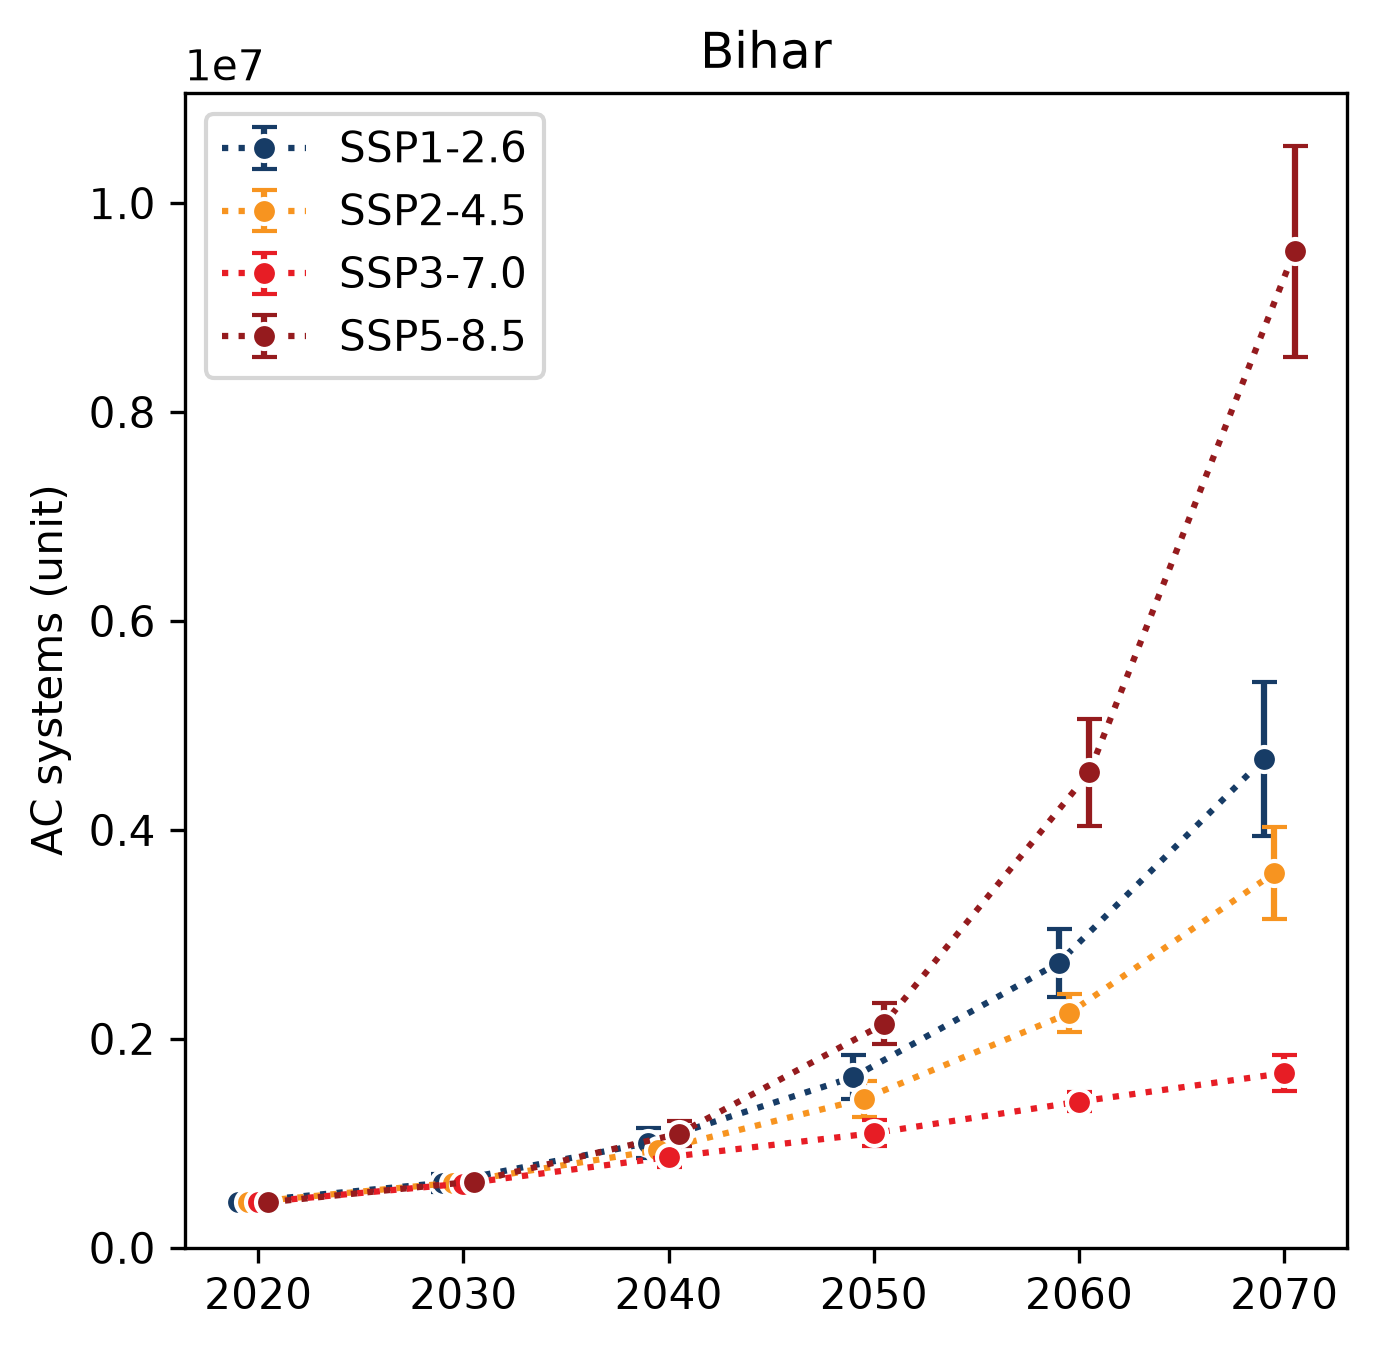
\includegraphics[height=0.25\textheight]{figures/projection_states/projection_ac_systems_Bihar.png}
   \caption{Projections des différentes variables pour Bihar}
\end{figure}

\clearpage

\subsubsection{Chhattisgarh}

\begin{figure}[ht]
   \centering
   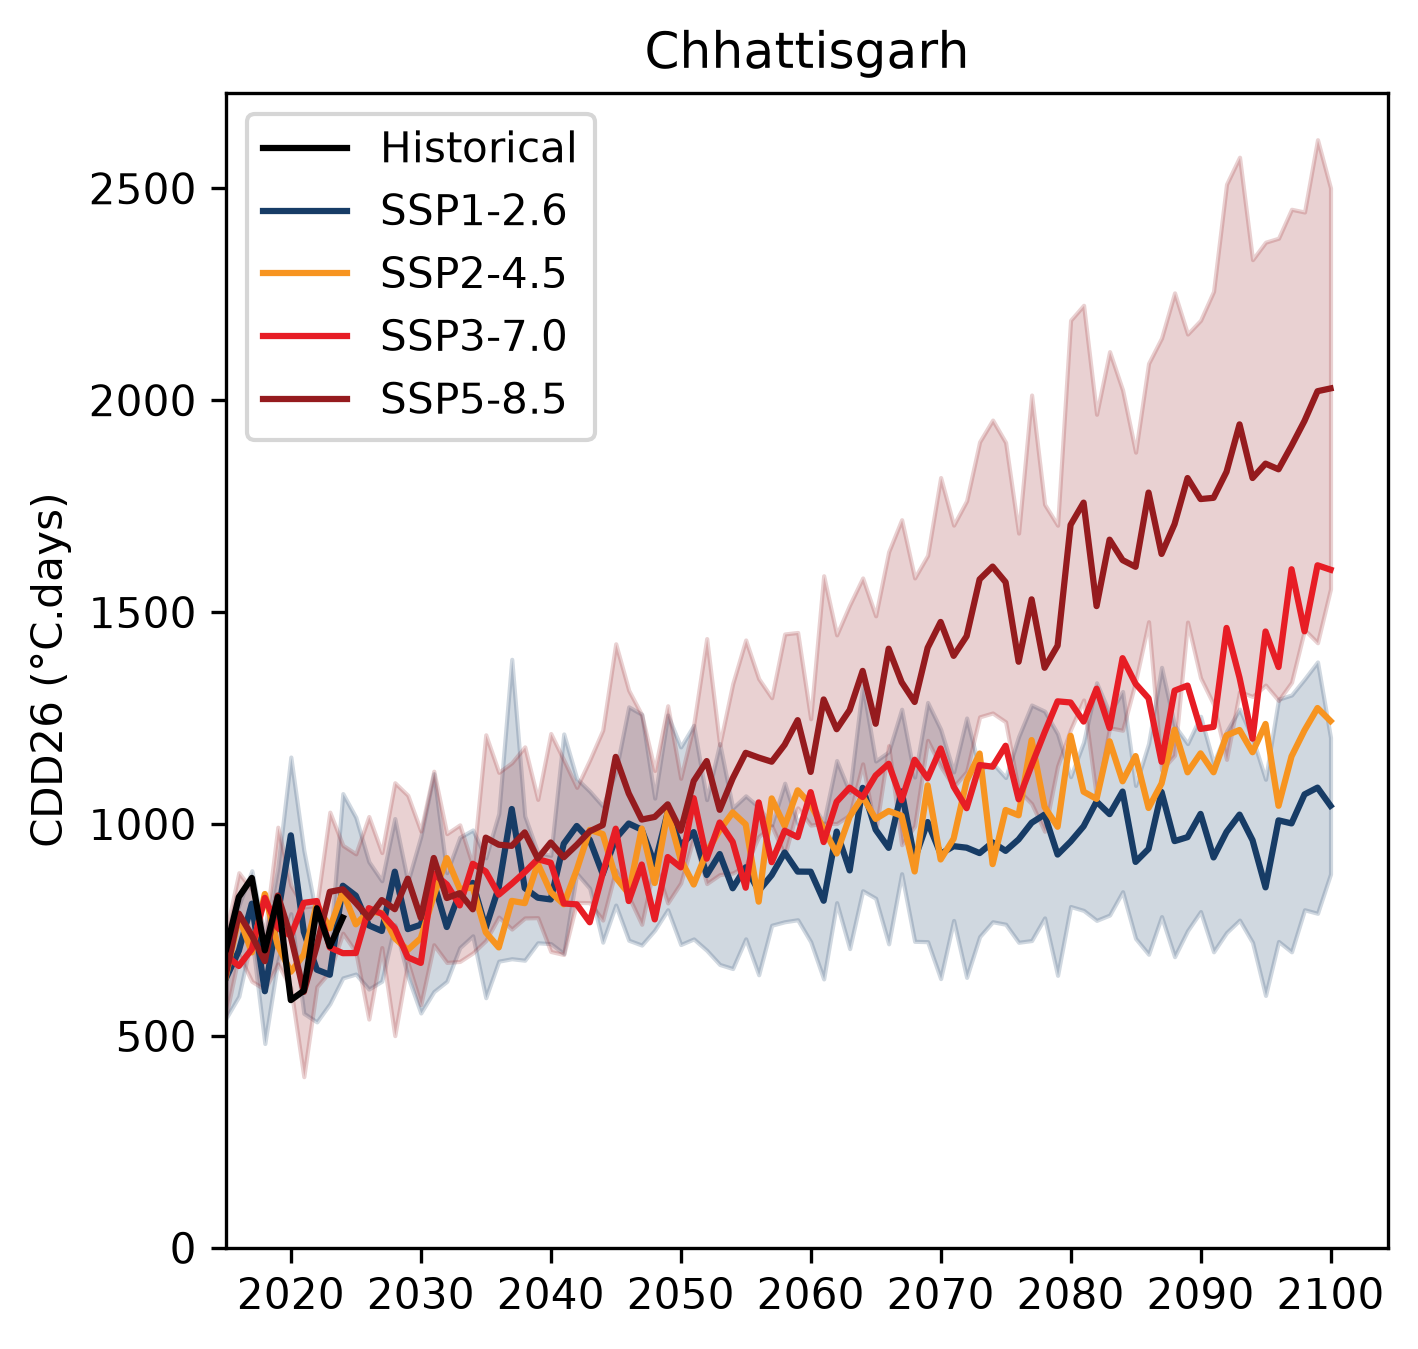
\includegraphics[height=0.25\textheight]{figures/projection_states/projection_cdd26_Chhattisgarh.png}\hfill
   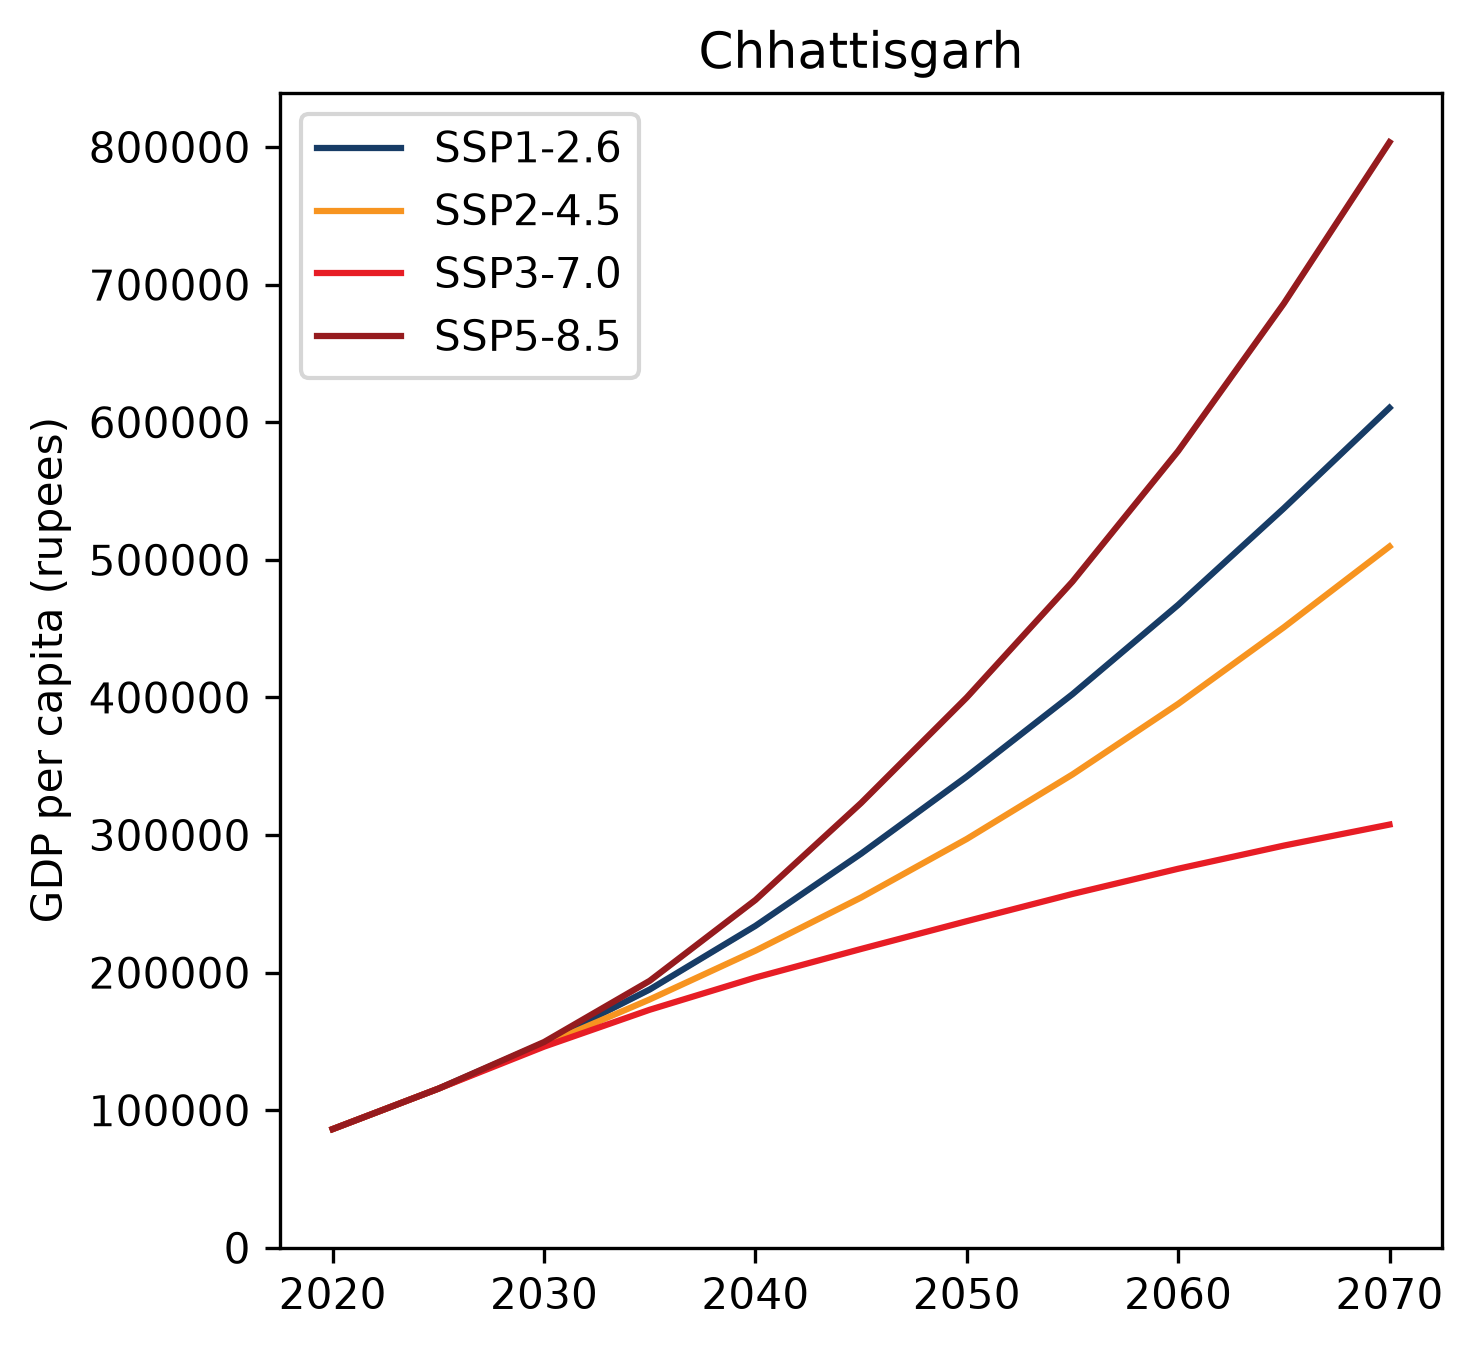
\includegraphics[height=0.25\textheight]{figures/projection_states/projection_gdp_per_capita_Chhattisgarh.png}\\
   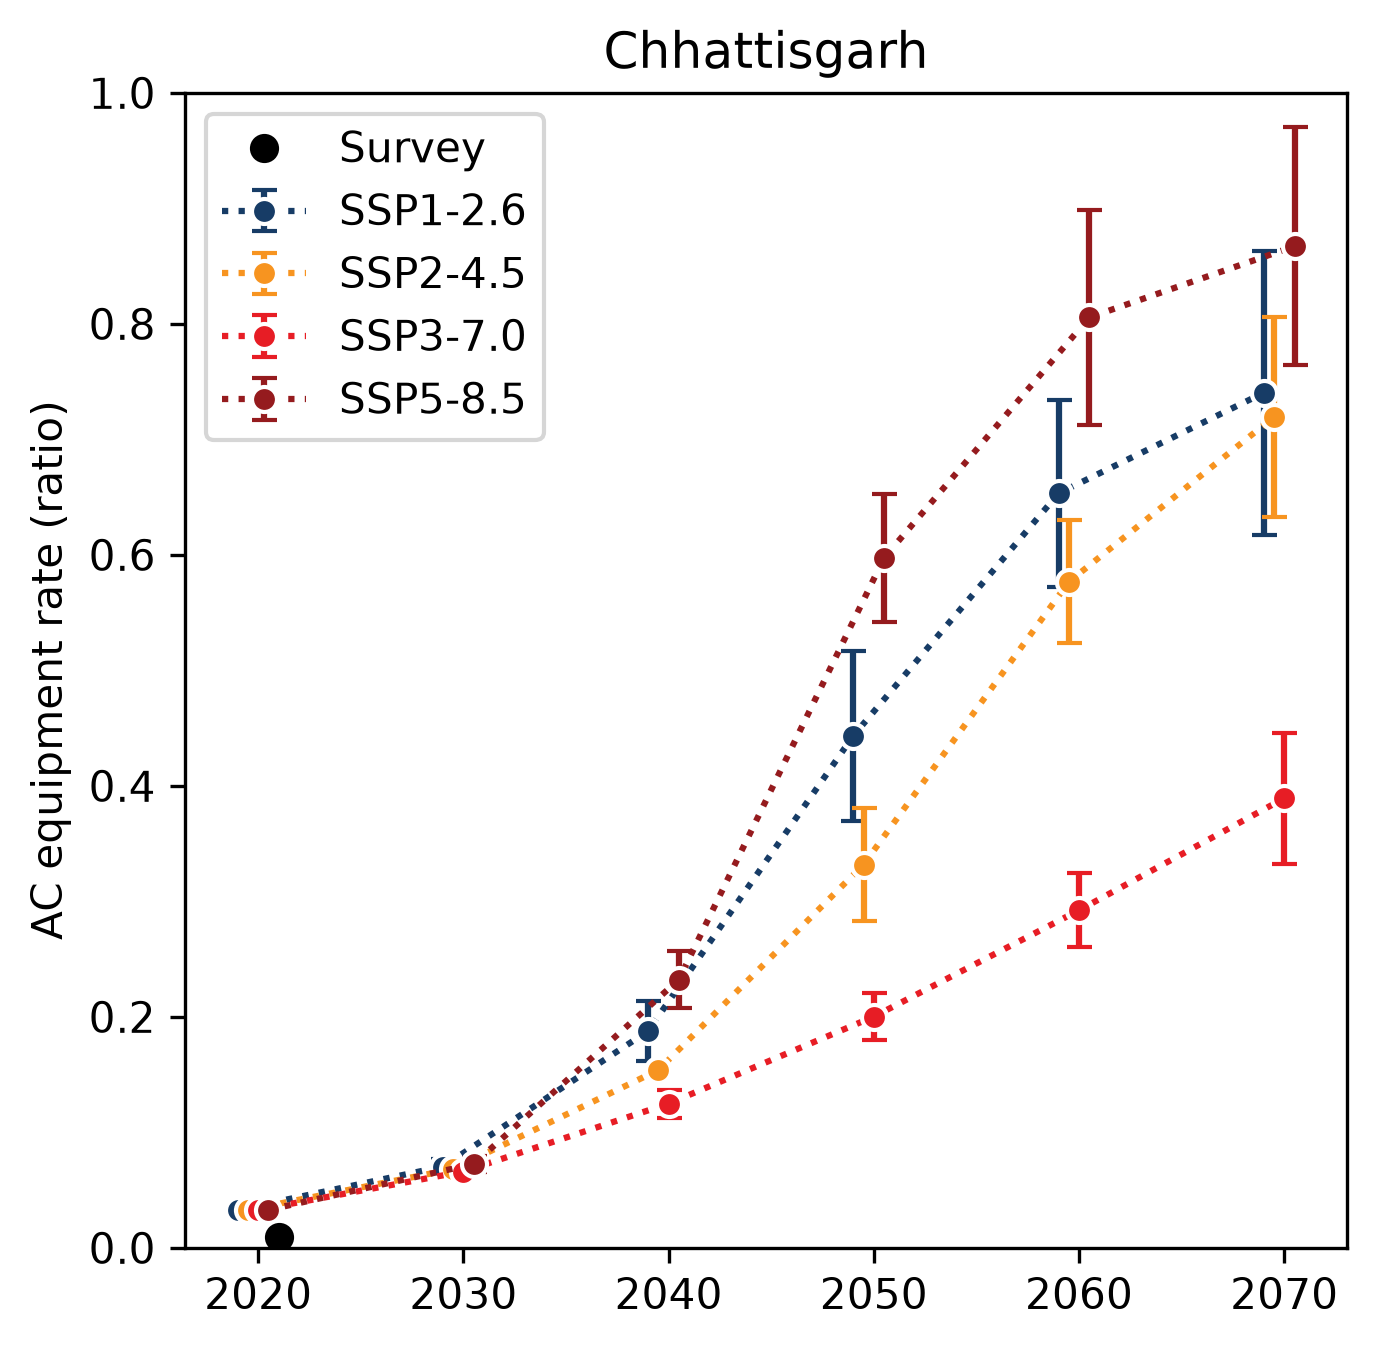
\includegraphics[height=0.25\textheight]{figures/projection_states/projection_ac_rate_Chhattisgarh.png}\hfill
   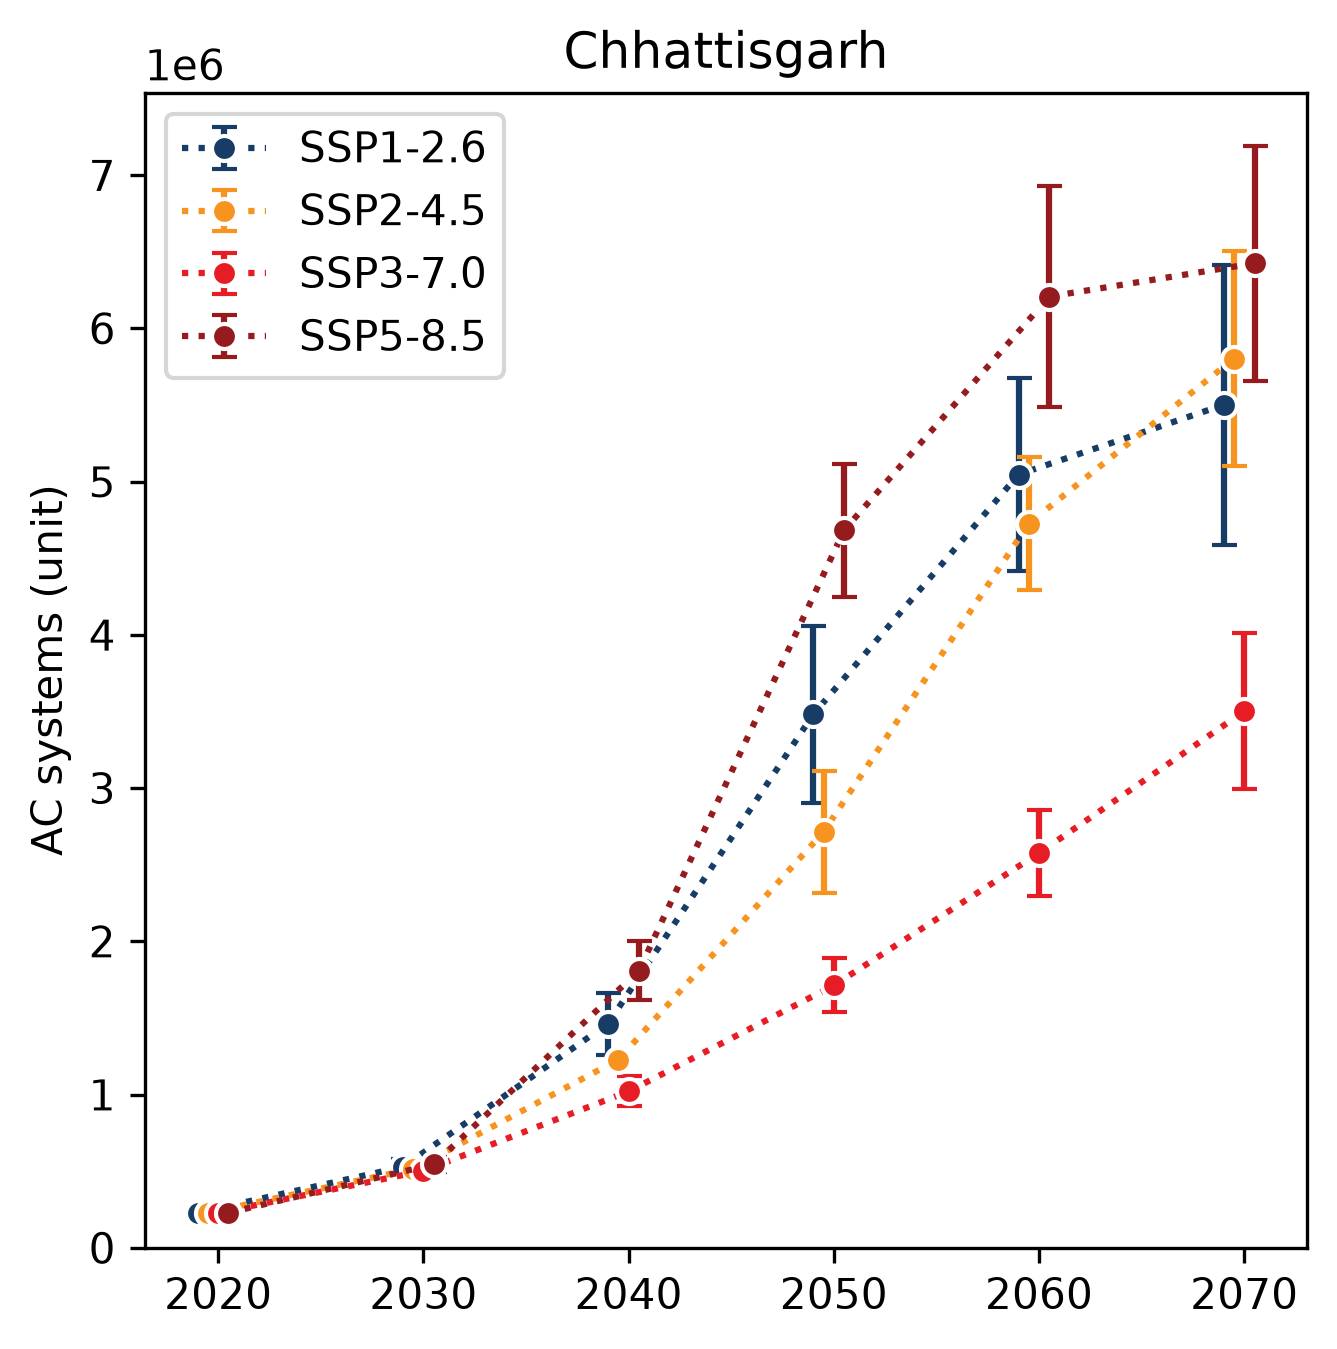
\includegraphics[height=0.25\textheight]{figures/projection_states/projection_ac_systems_Chhattisgarh.png}
   \caption{Projections des différentes variables pour Chhattisgarh}
\end{figure}

\clearpage

\subsubsection{Delhi}

\begin{figure}[ht]
   \centering
   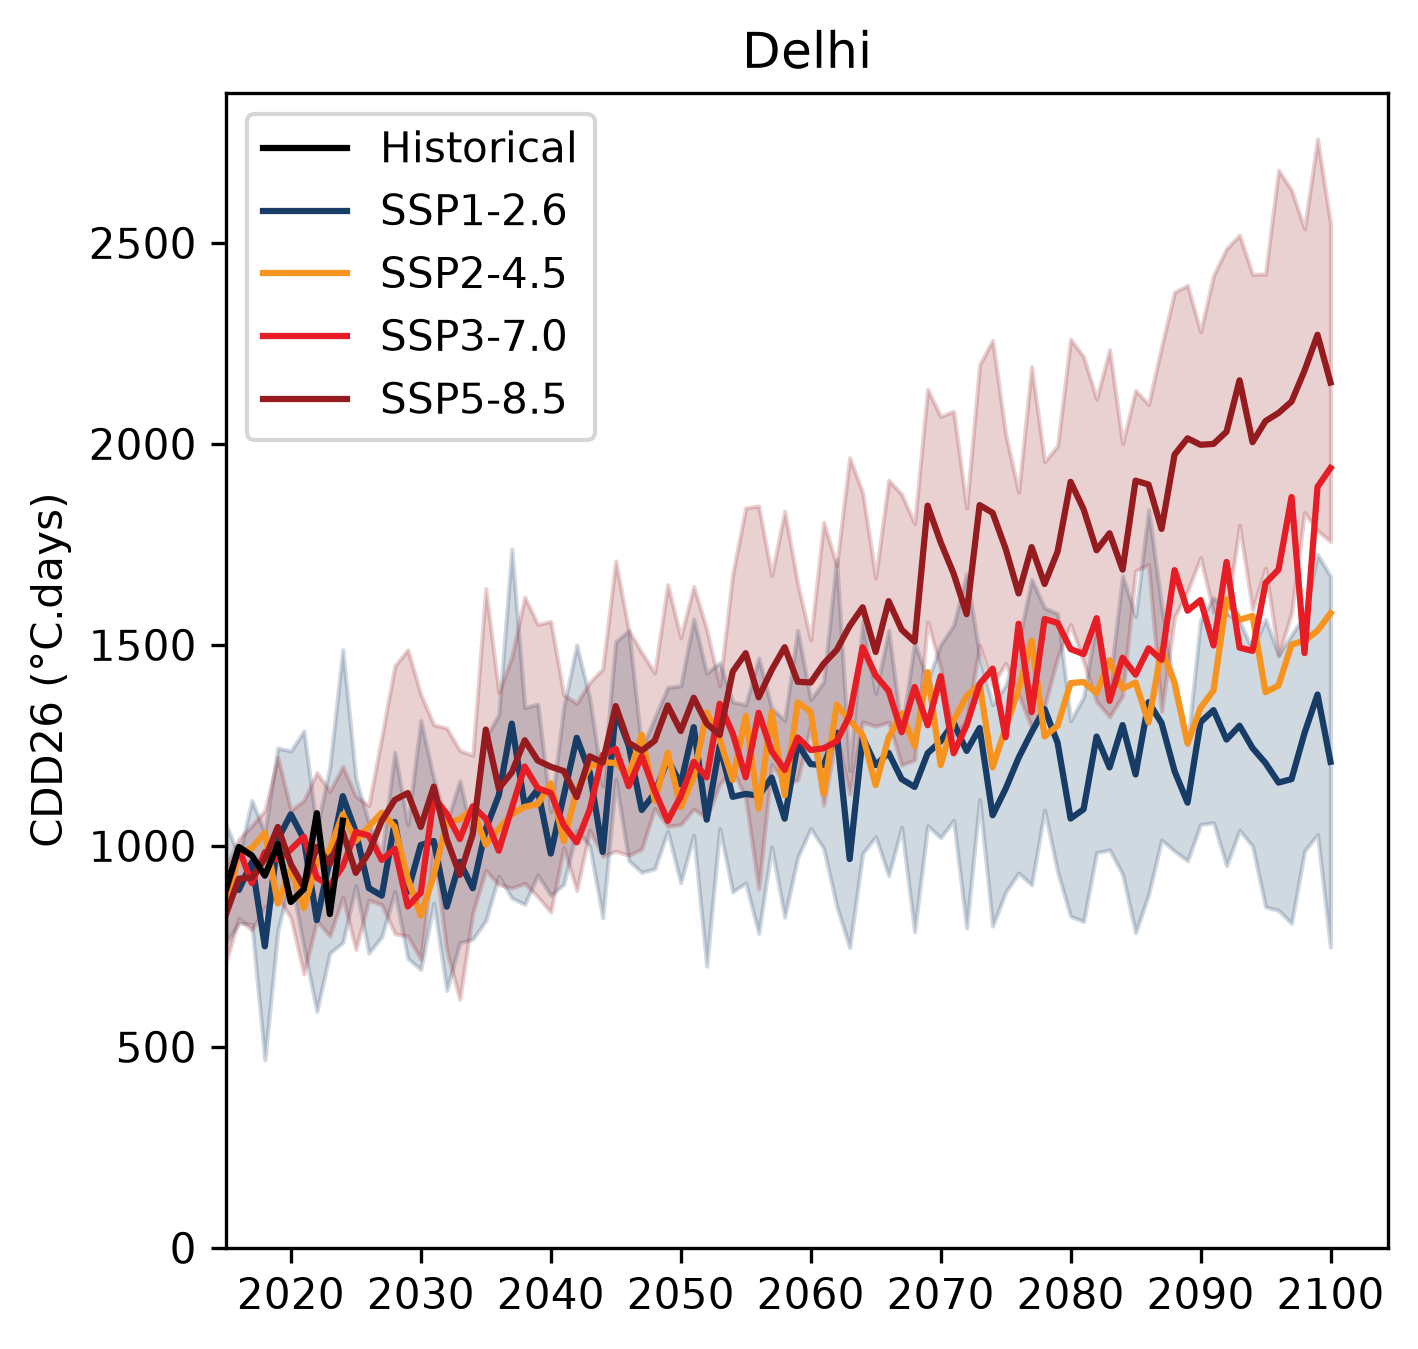
\includegraphics[height=0.25\textheight]{figures/projection_states/projection_cdd26_Delhi.png}\hfill
   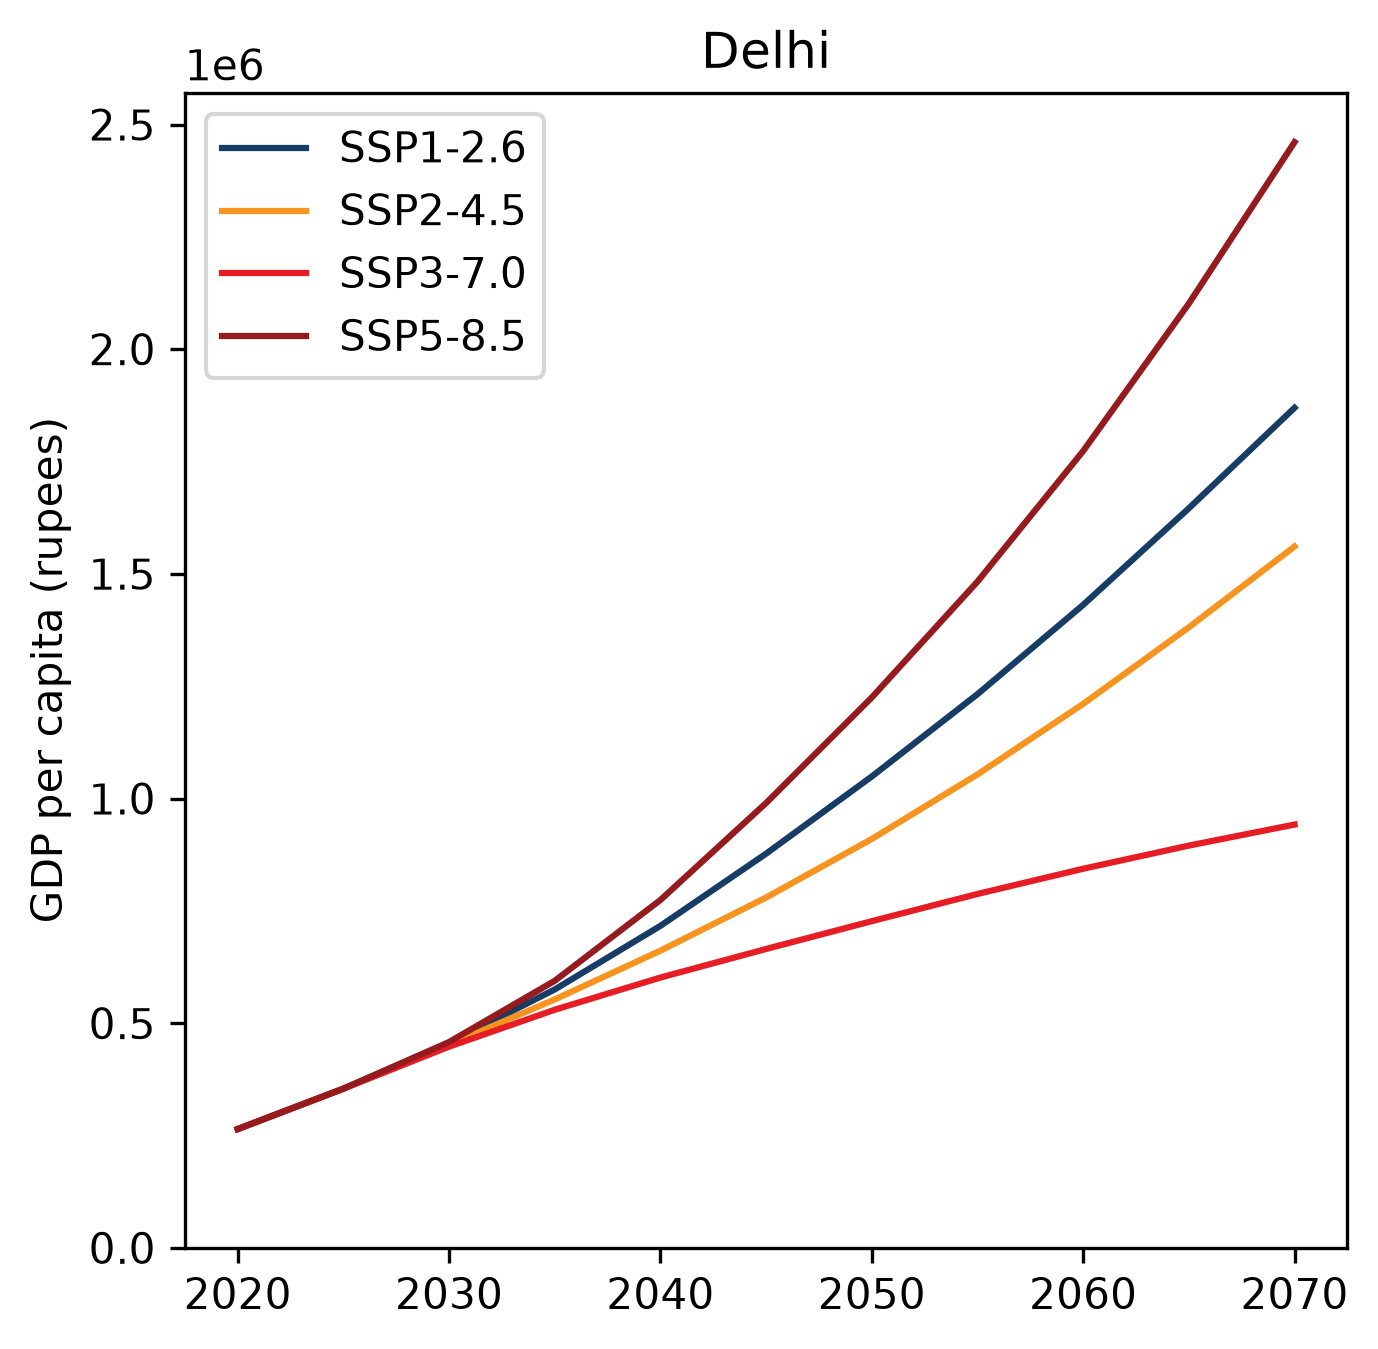
\includegraphics[height=0.25\textheight]{figures/projection_states/projection_gdp_per_capita_Delhi.png}\\
   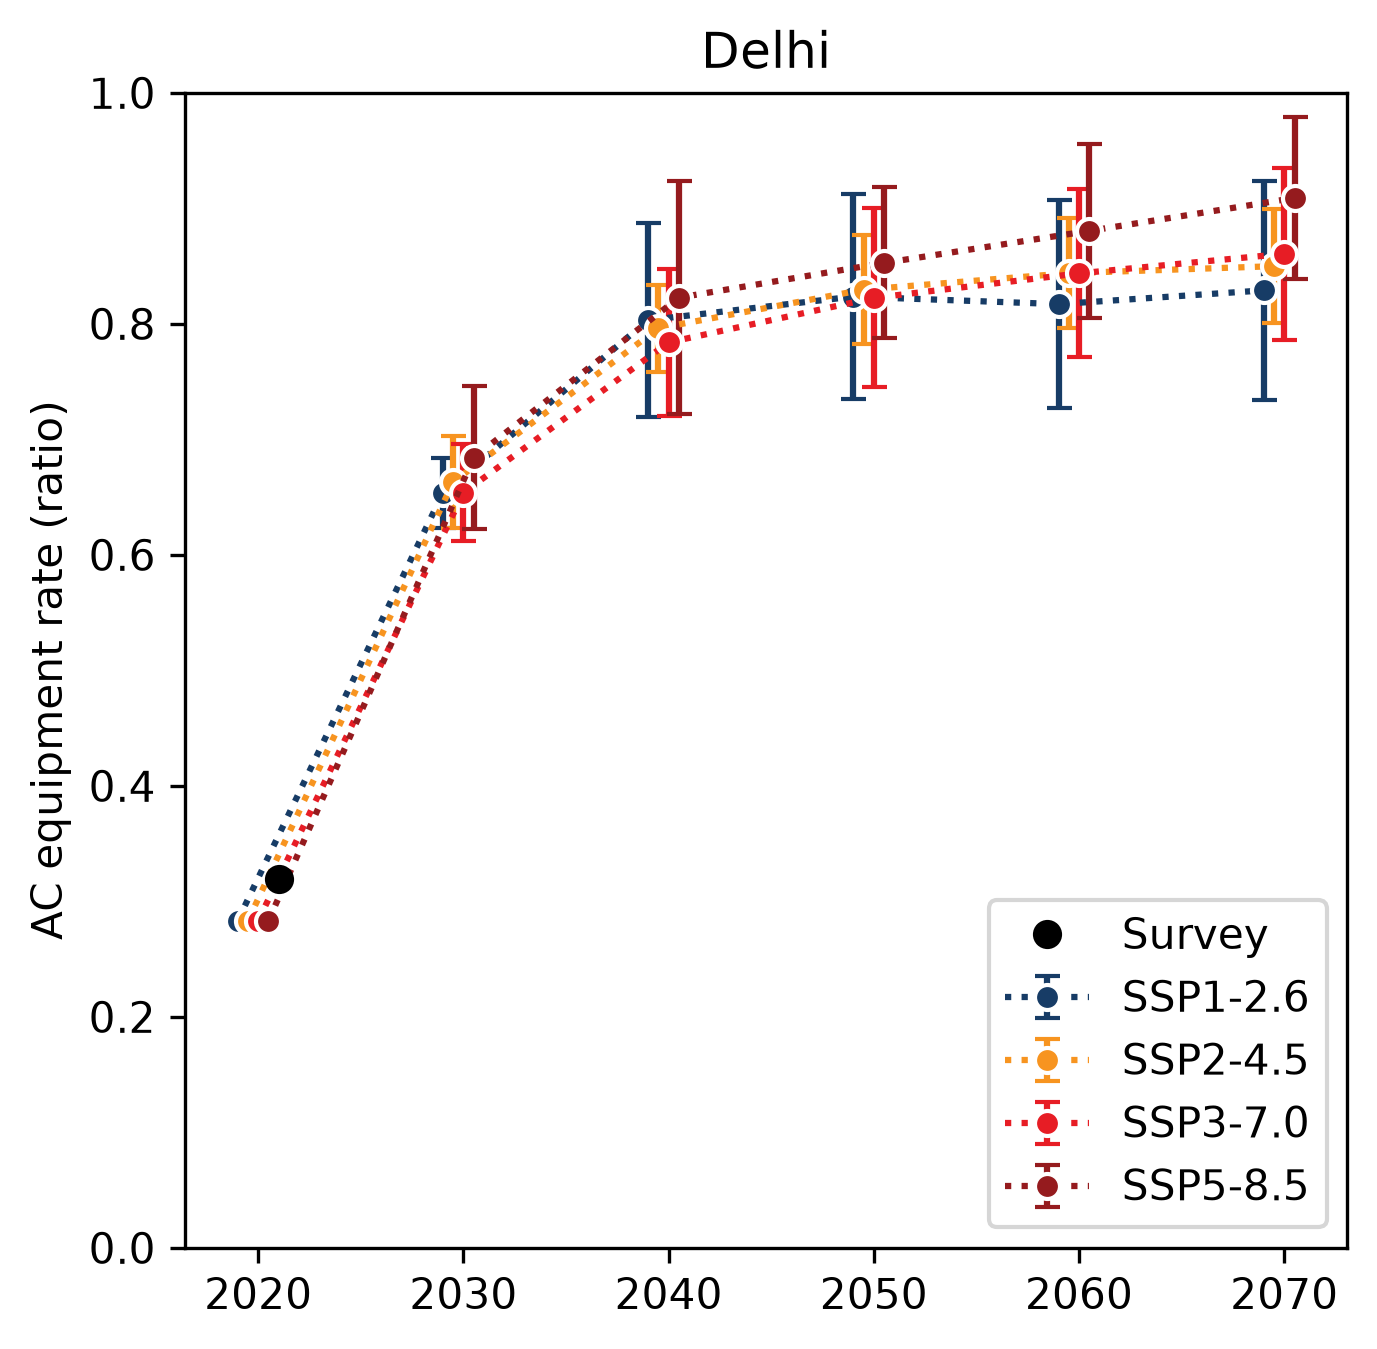
\includegraphics[height=0.25\textheight]{figures/projection_states/projection_ac_rate_Delhi.png}\hfill
   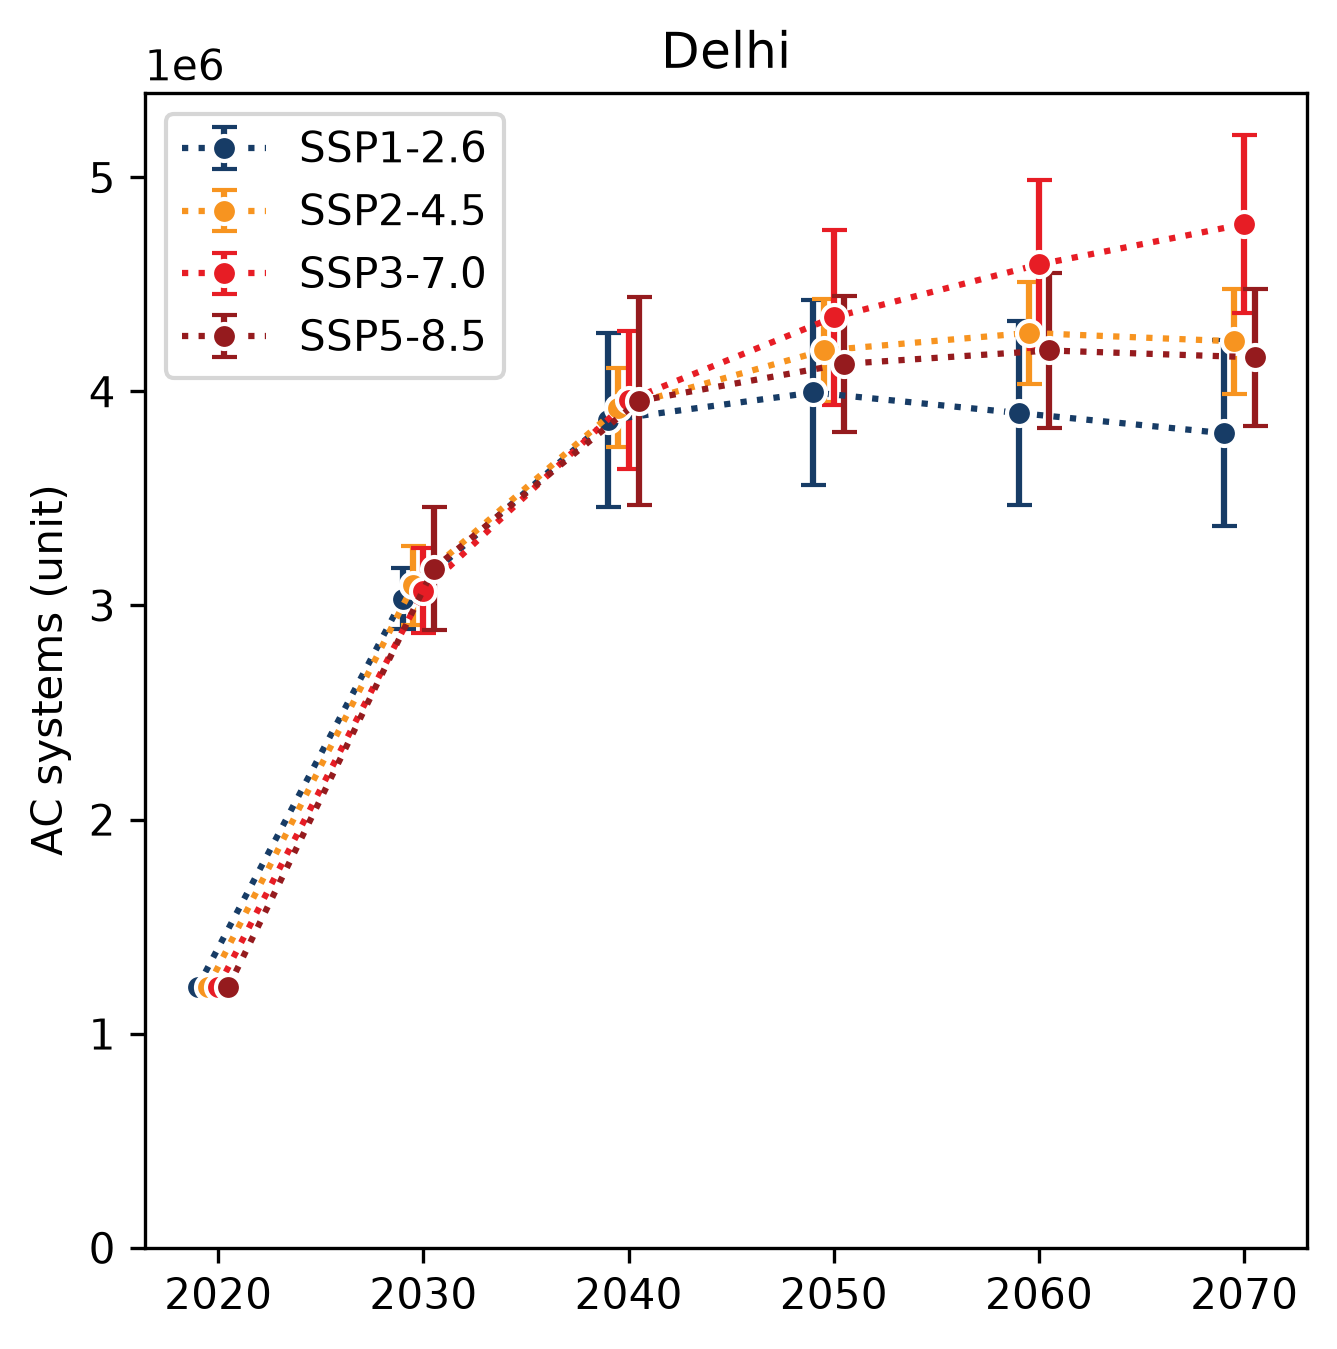
\includegraphics[height=0.25\textheight]{figures/projection_states/projection_ac_systems_Delhi.png}
   \caption{Projections des différentes variables pour Delhi}
\end{figure}

\clearpage

\subsubsection{Goa}

\begin{figure}[ht]
   \centering
   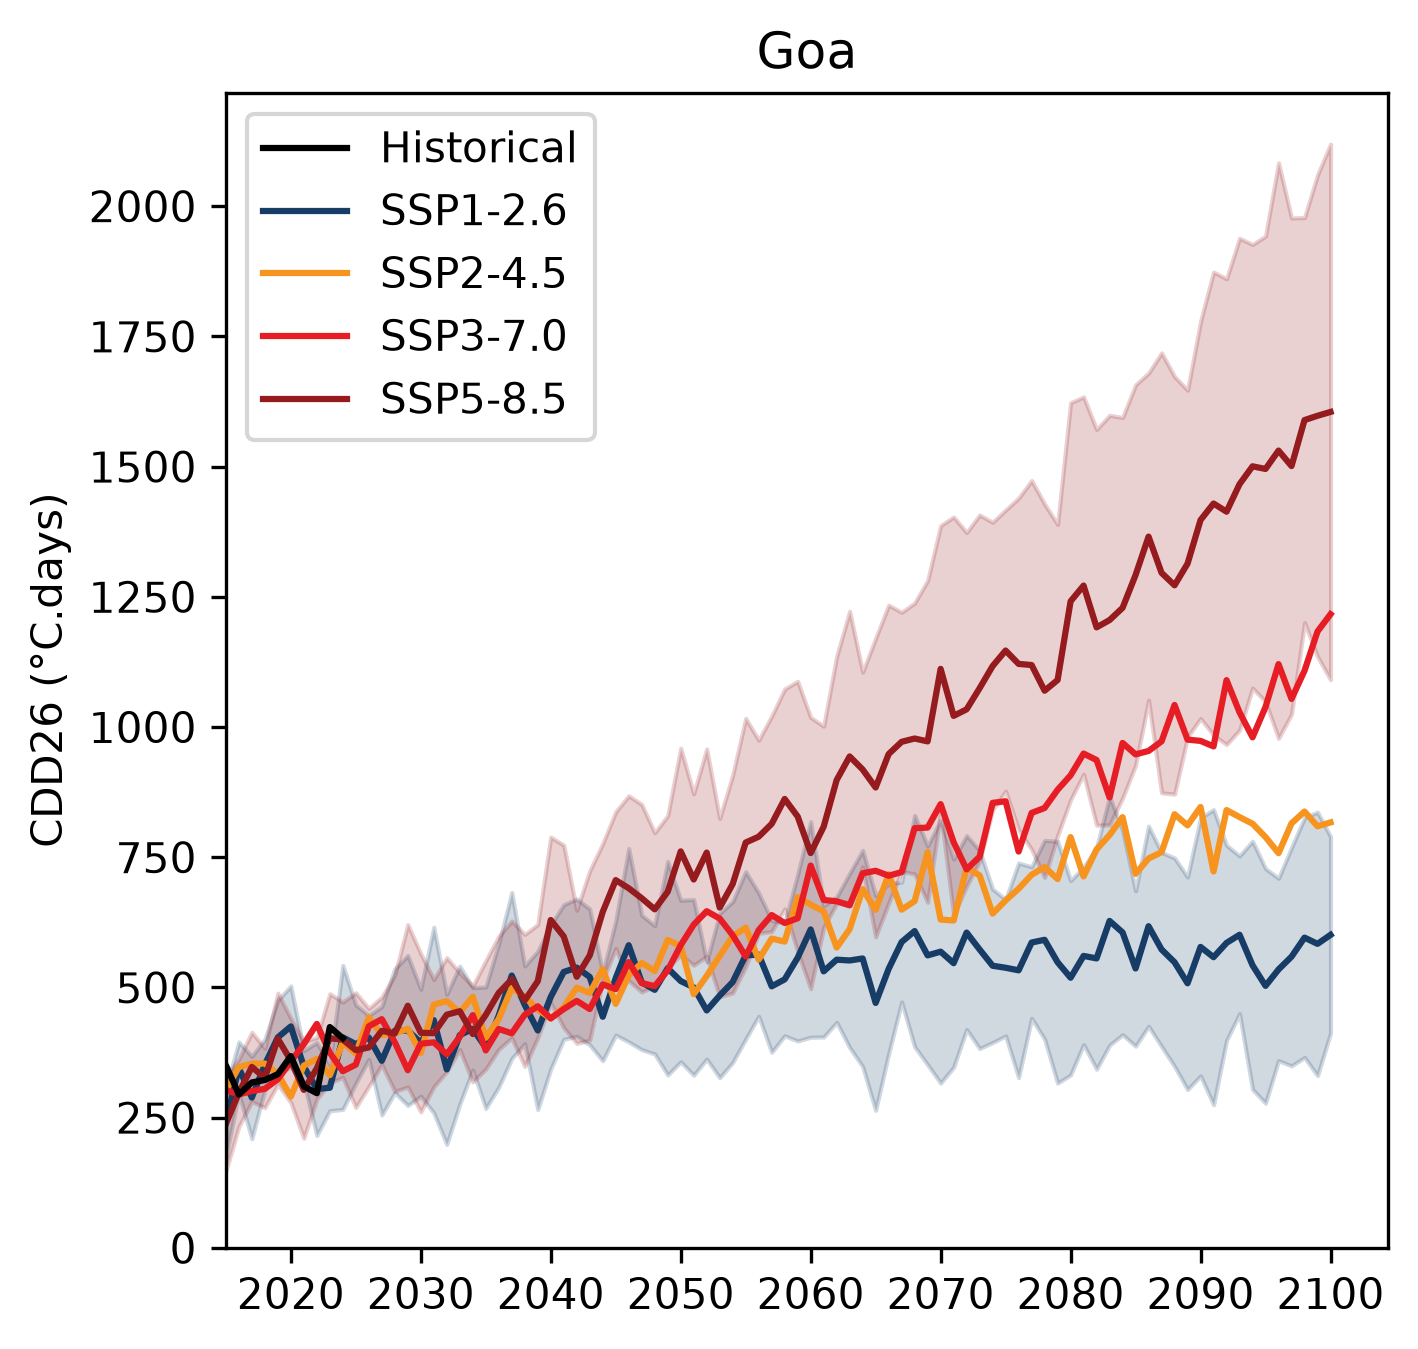
\includegraphics[height=0.25\textheight]{figures/projection_states/projection_cdd26_Goa.png}\hfill
   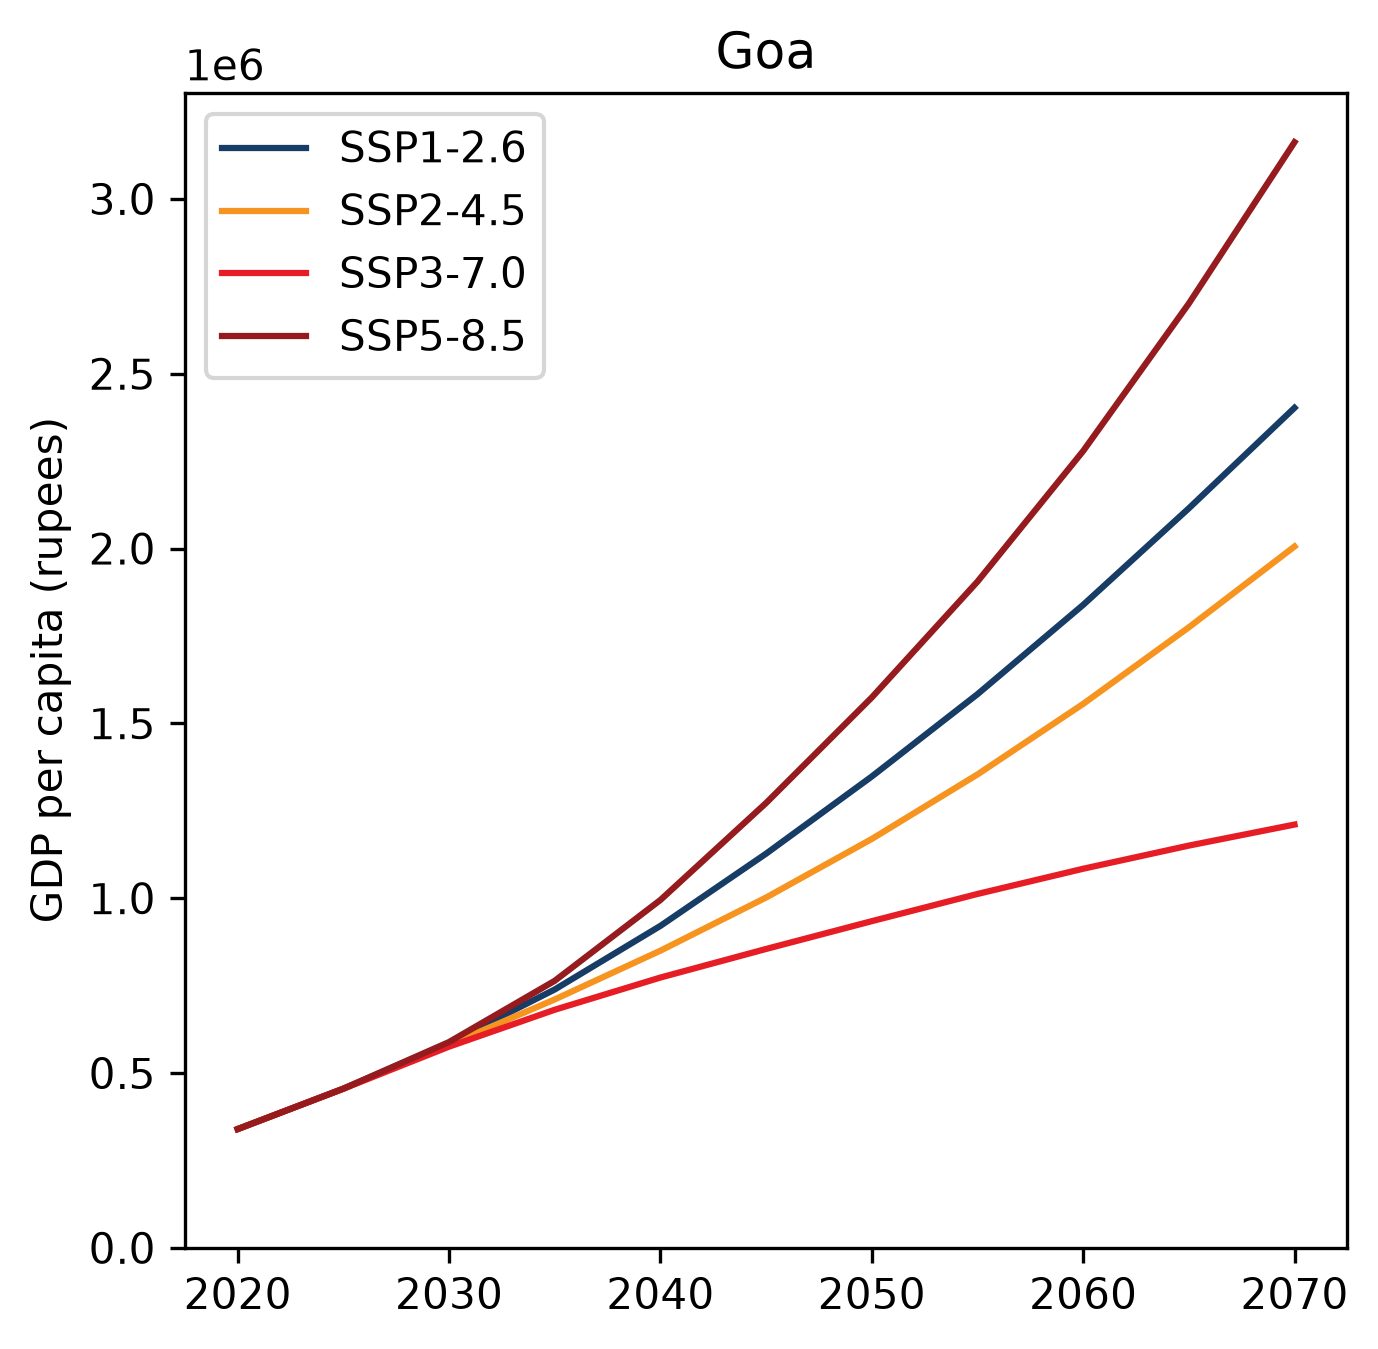
\includegraphics[height=0.25\textheight]{figures/projection_states/projection_gdp_per_capita_Goa.png}\\
   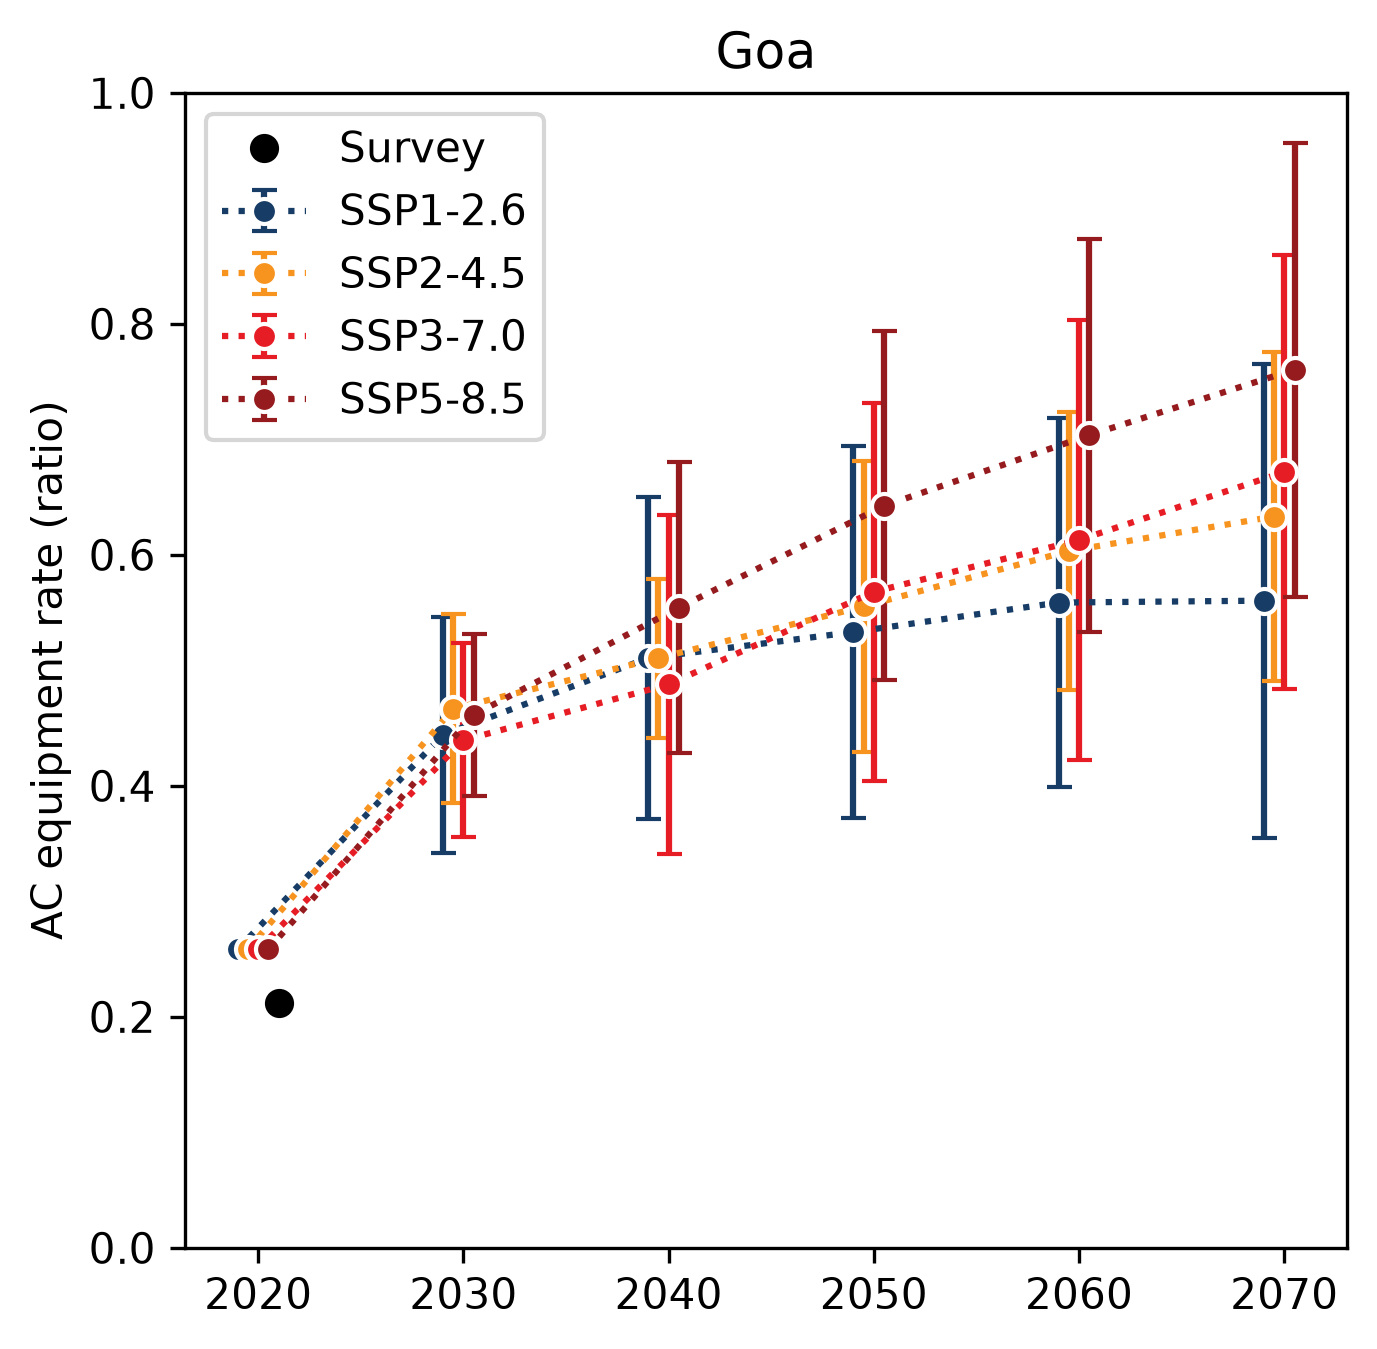
\includegraphics[height=0.25\textheight]{figures/projection_states/projection_ac_rate_Goa.png}\hfill
   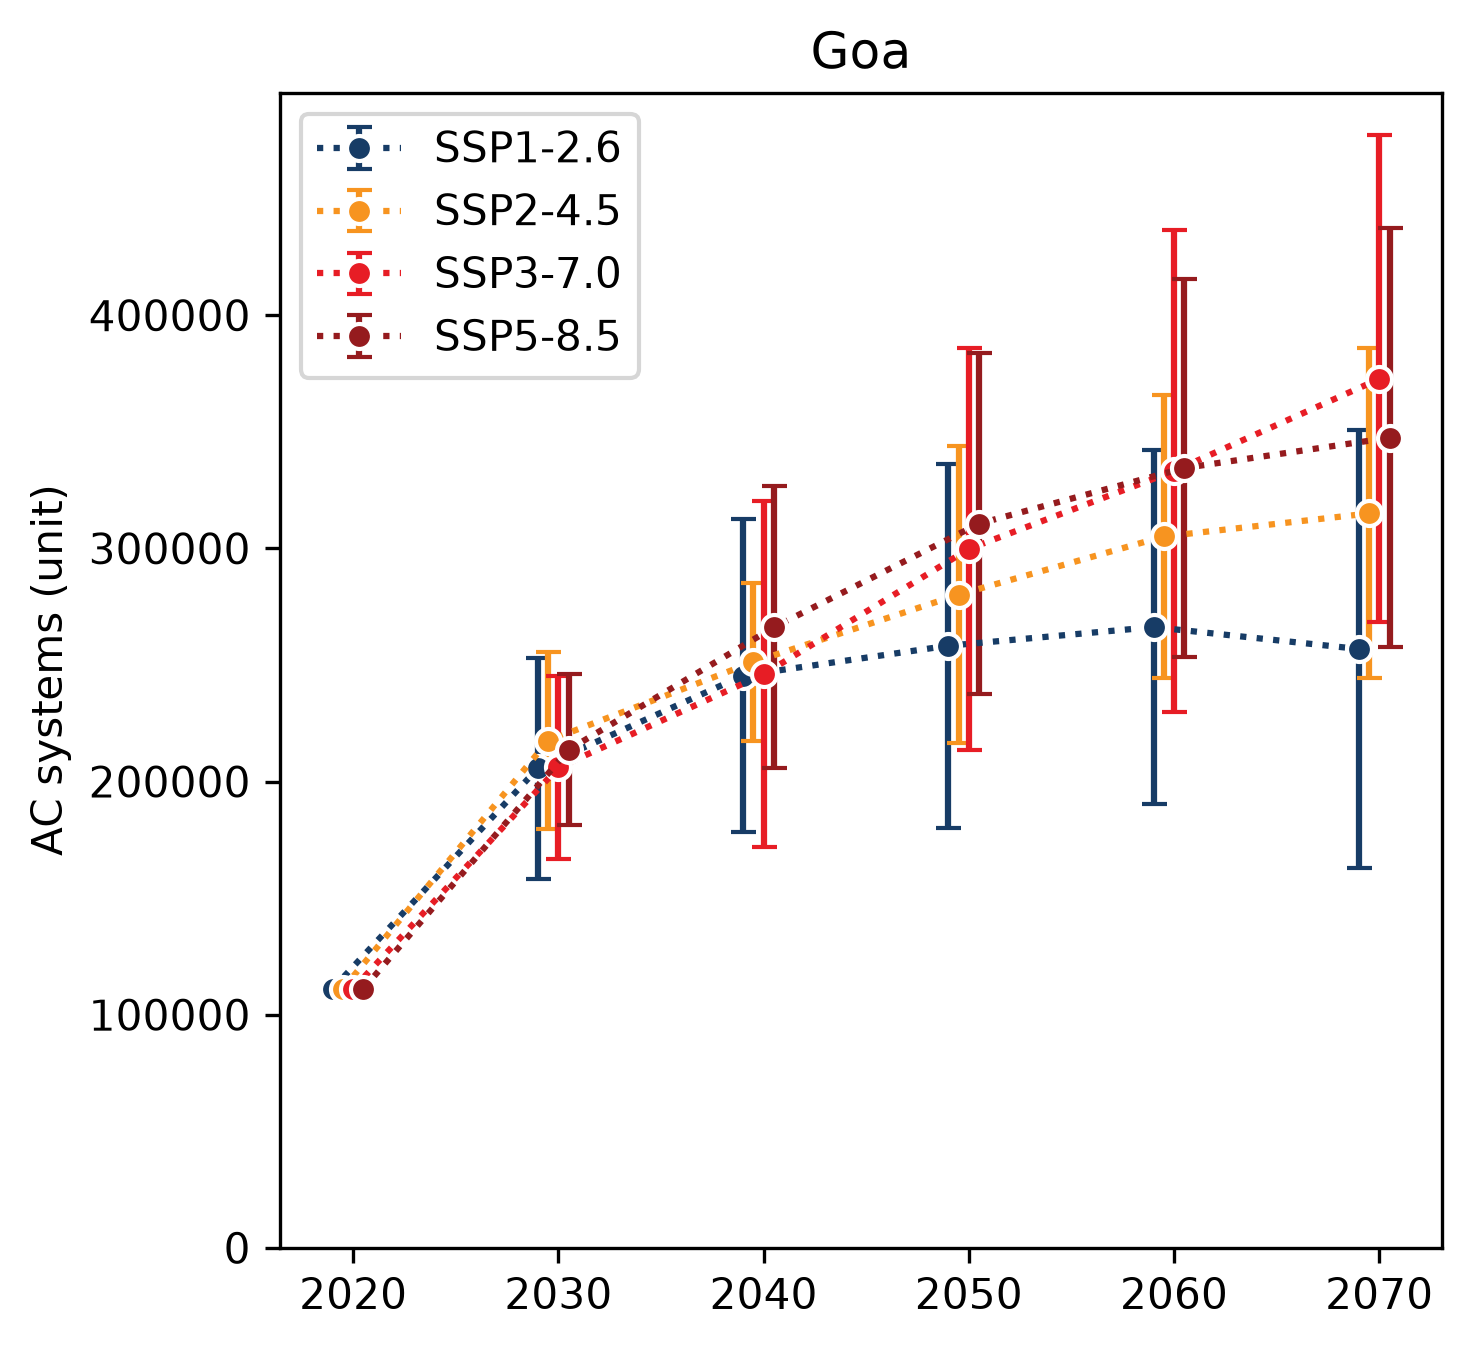
\includegraphics[height=0.25\textheight]{figures/projection_states/projection_ac_systems_Goa.png}
   \caption{Projections des différentes variables pour Goa}
\end{figure}

\clearpage

\subsubsection{Gujarat}

\begin{figure}[ht]
   \centering
   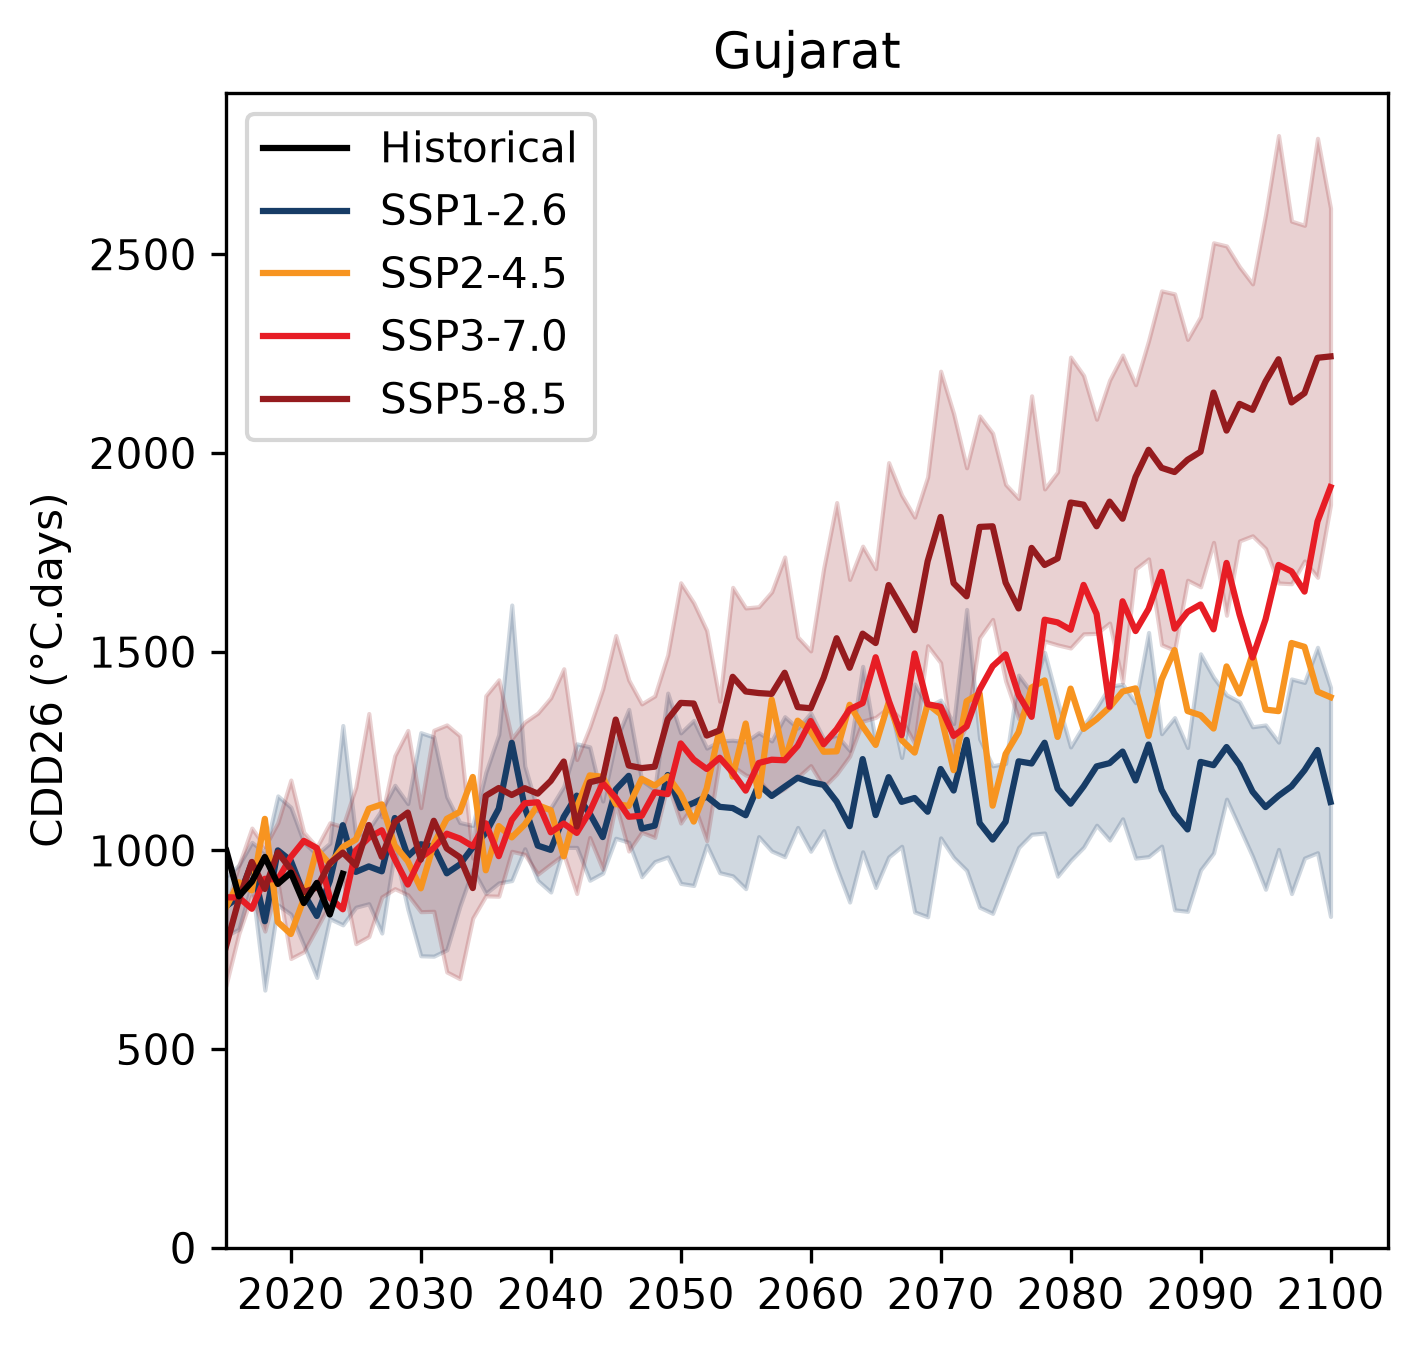
\includegraphics[height=0.25\textheight]{figures/projection_states/projection_cdd26_Gujarat.png}\hfill
   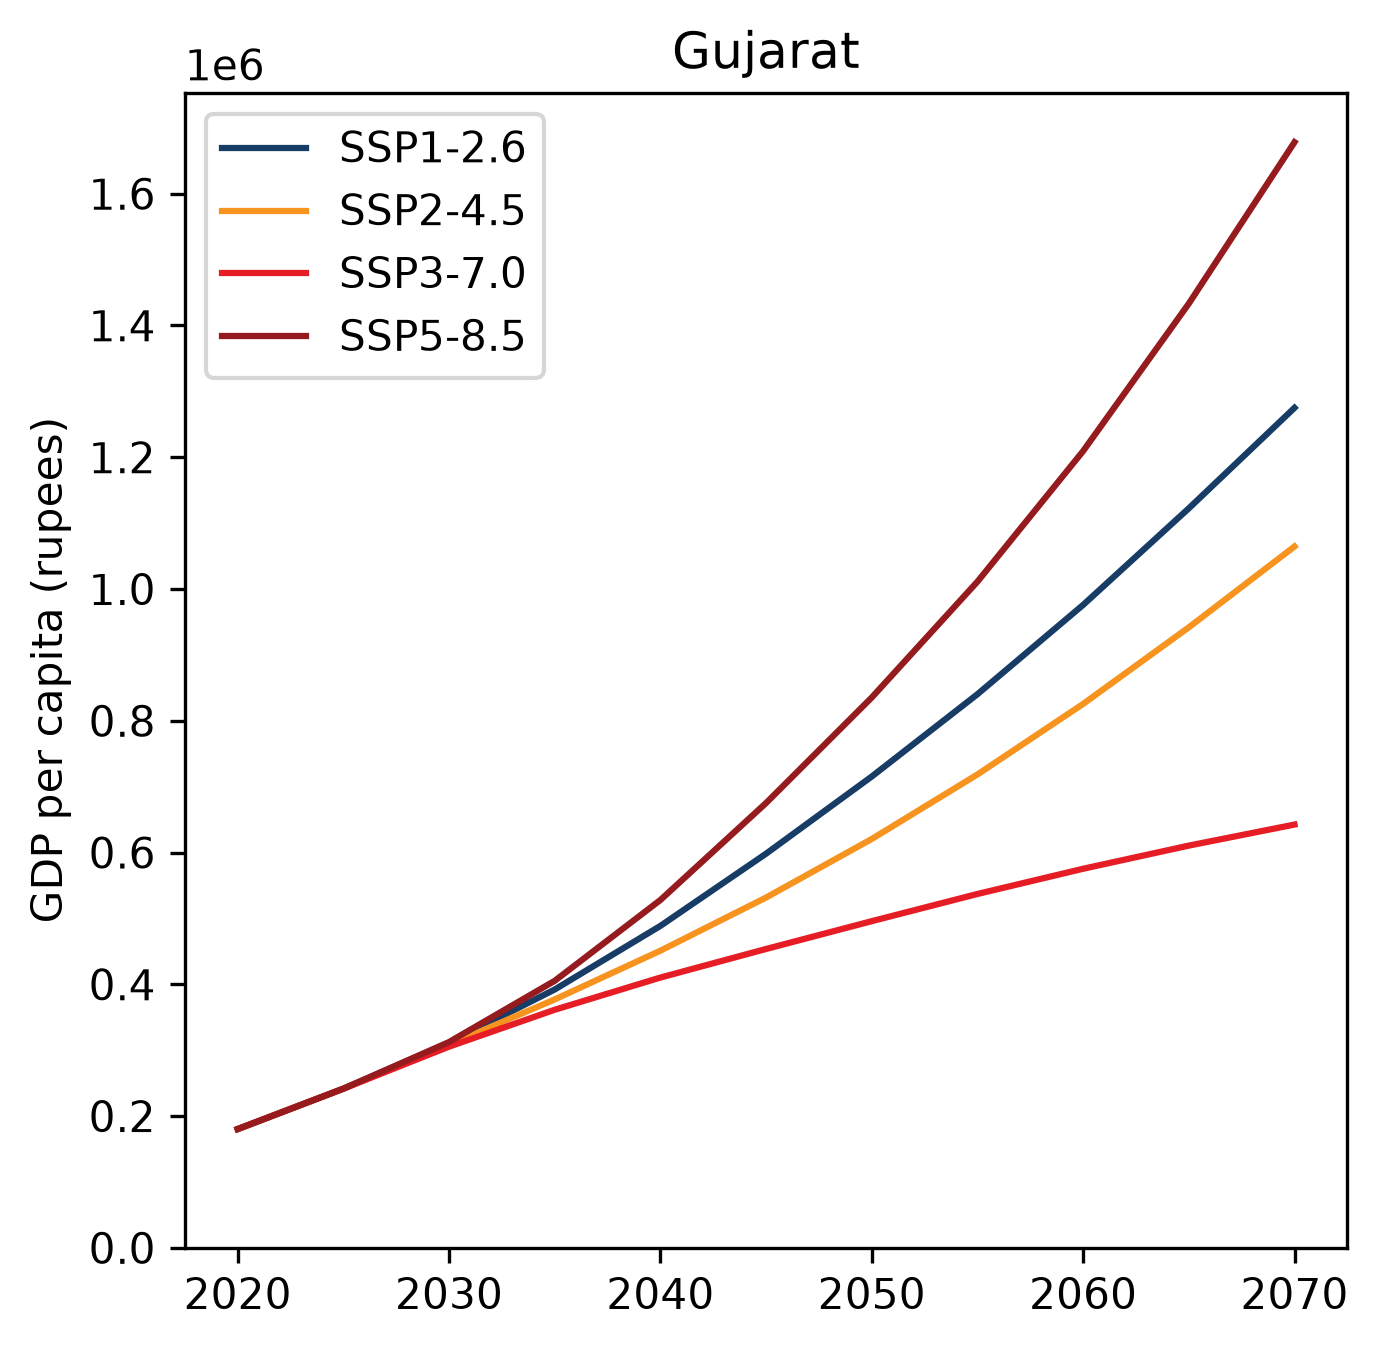
\includegraphics[height=0.25\textheight]{figures/projection_states/projection_gdp_per_capita_Gujarat.png}\\
   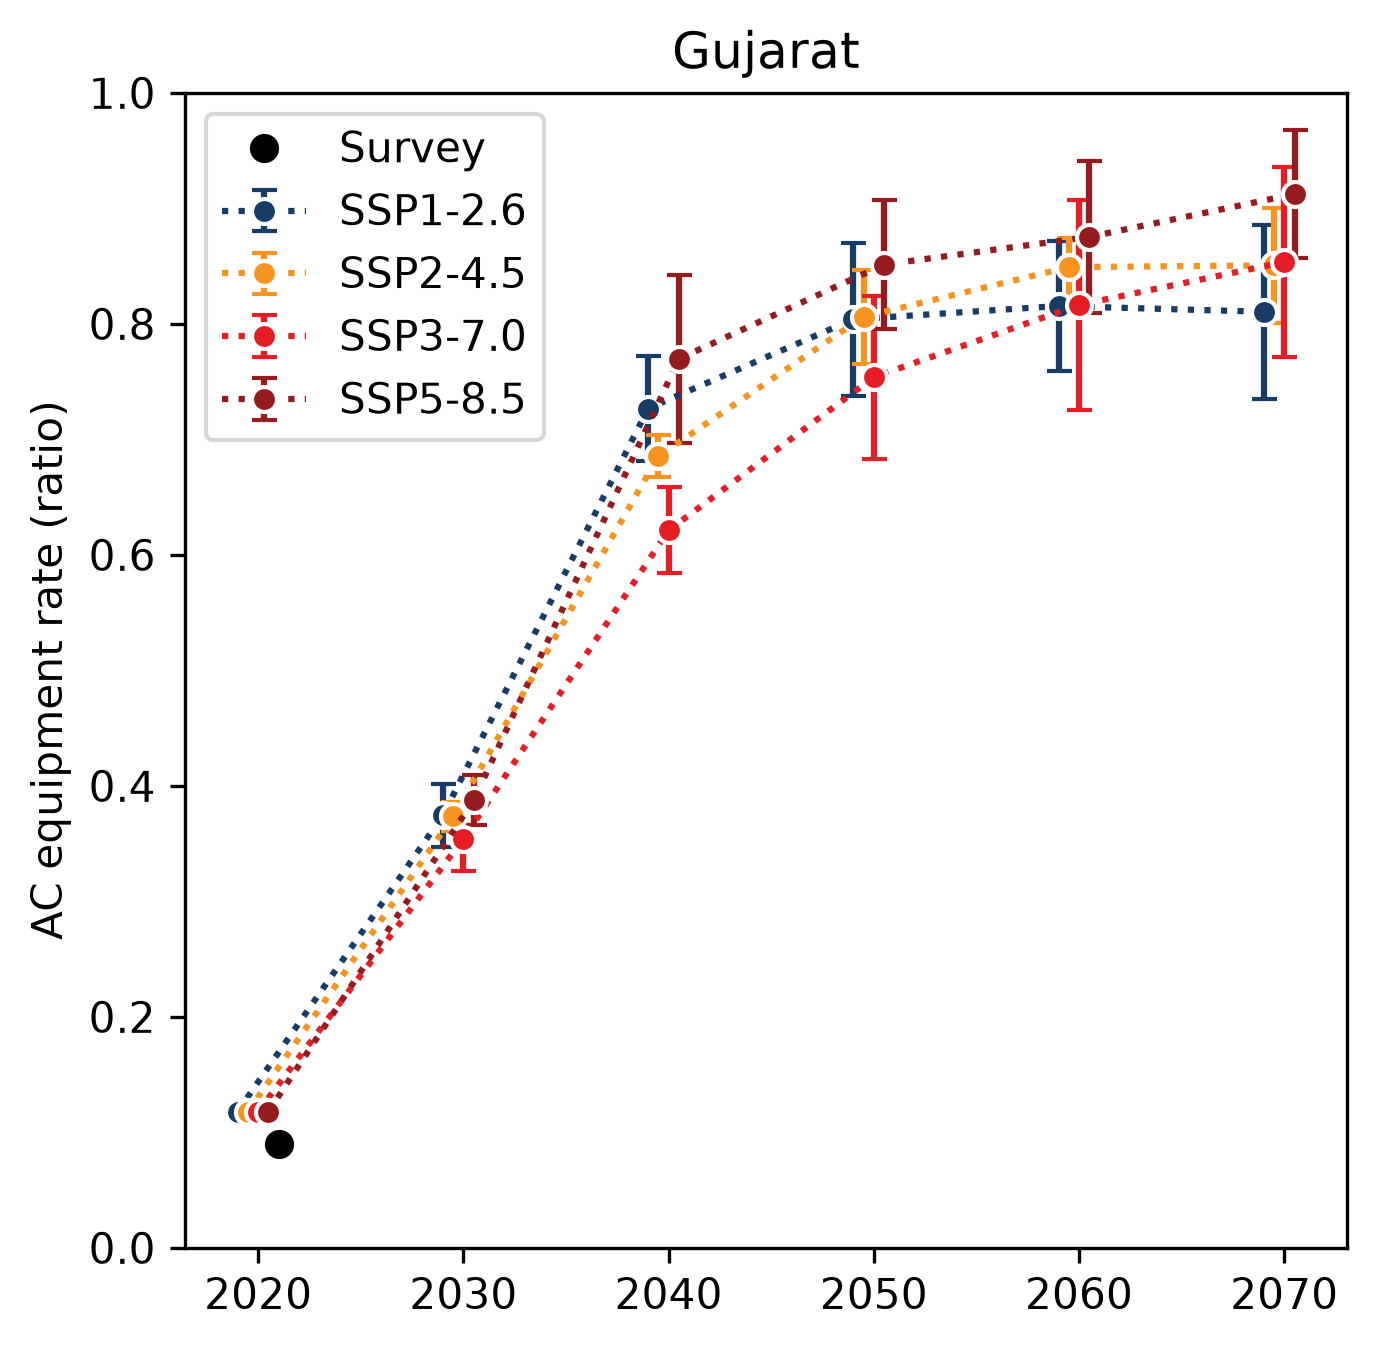
\includegraphics[height=0.25\textheight]{figures/projection_states/projection_ac_rate_Gujarat.png}\hfill
   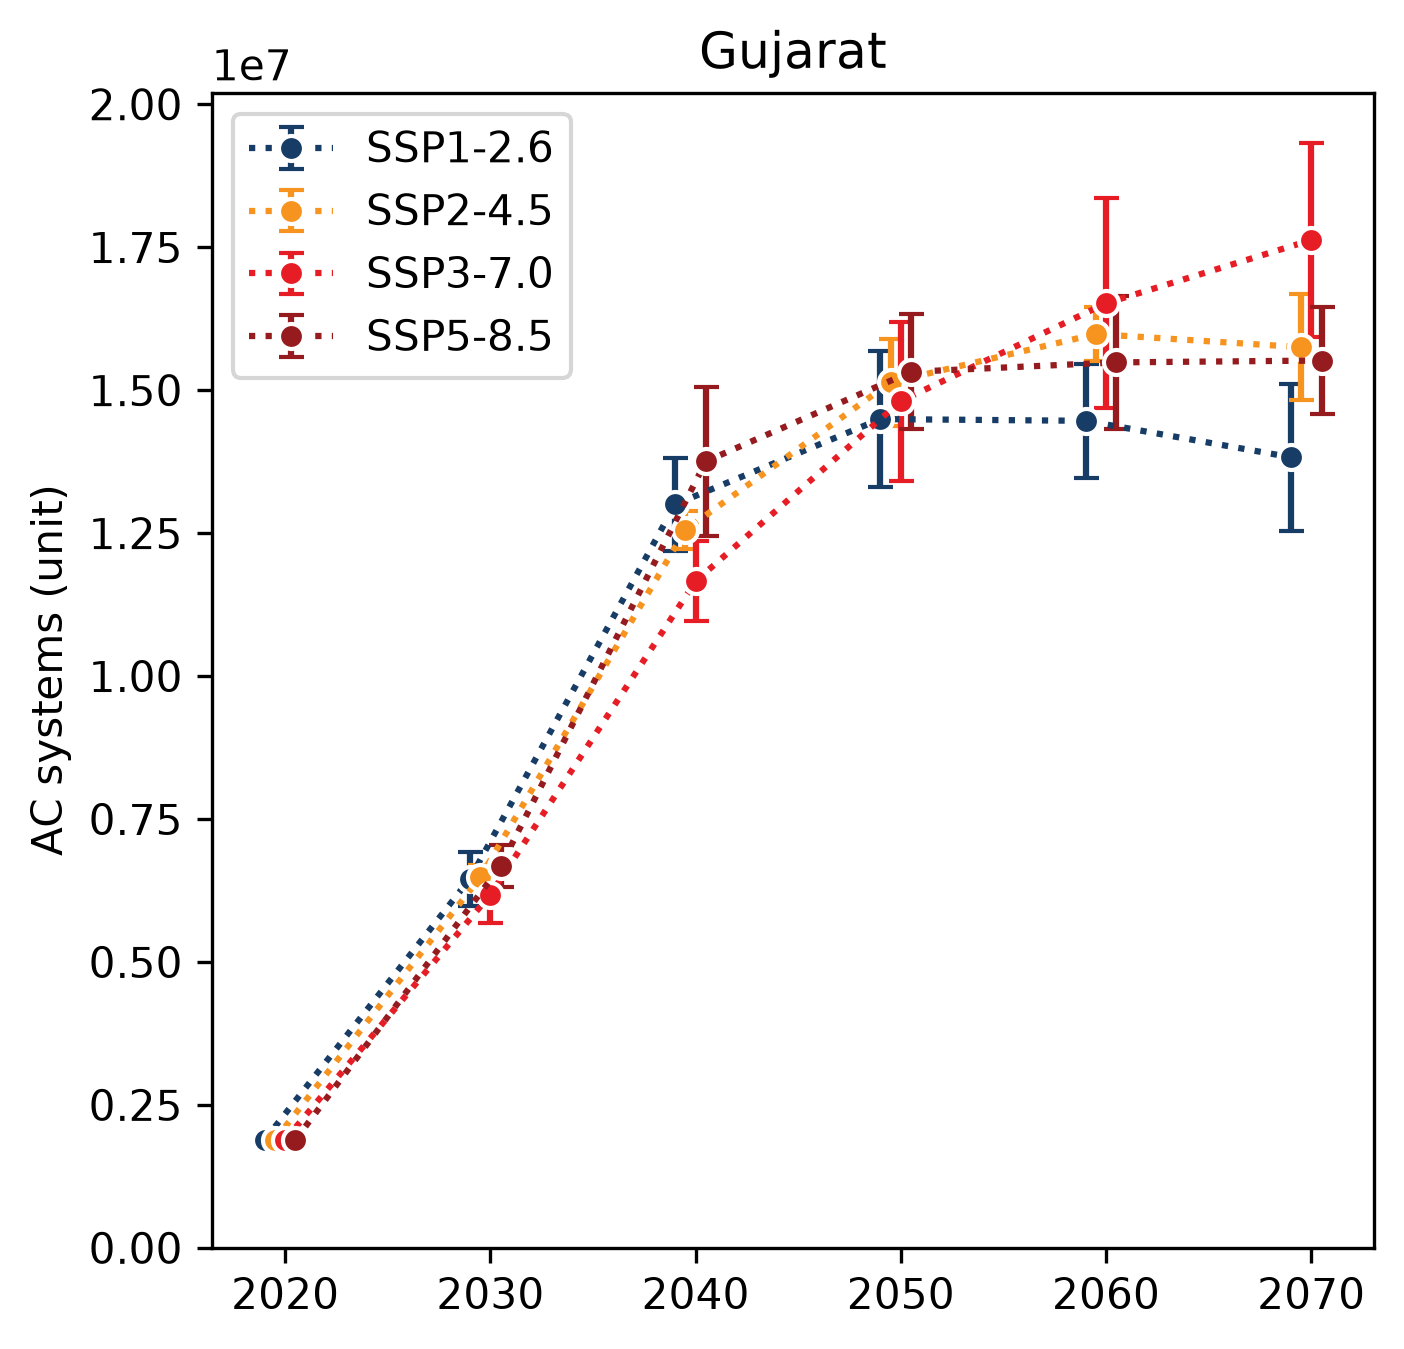
\includegraphics[height=0.25\textheight]{figures/projection_states/projection_ac_systems_Gujarat.png}
   \caption{Projections des différentes variables pour Gujarat}
\end{figure}

\clearpage

\subsubsection{Haryana}

\begin{figure}[ht]
   \centering
   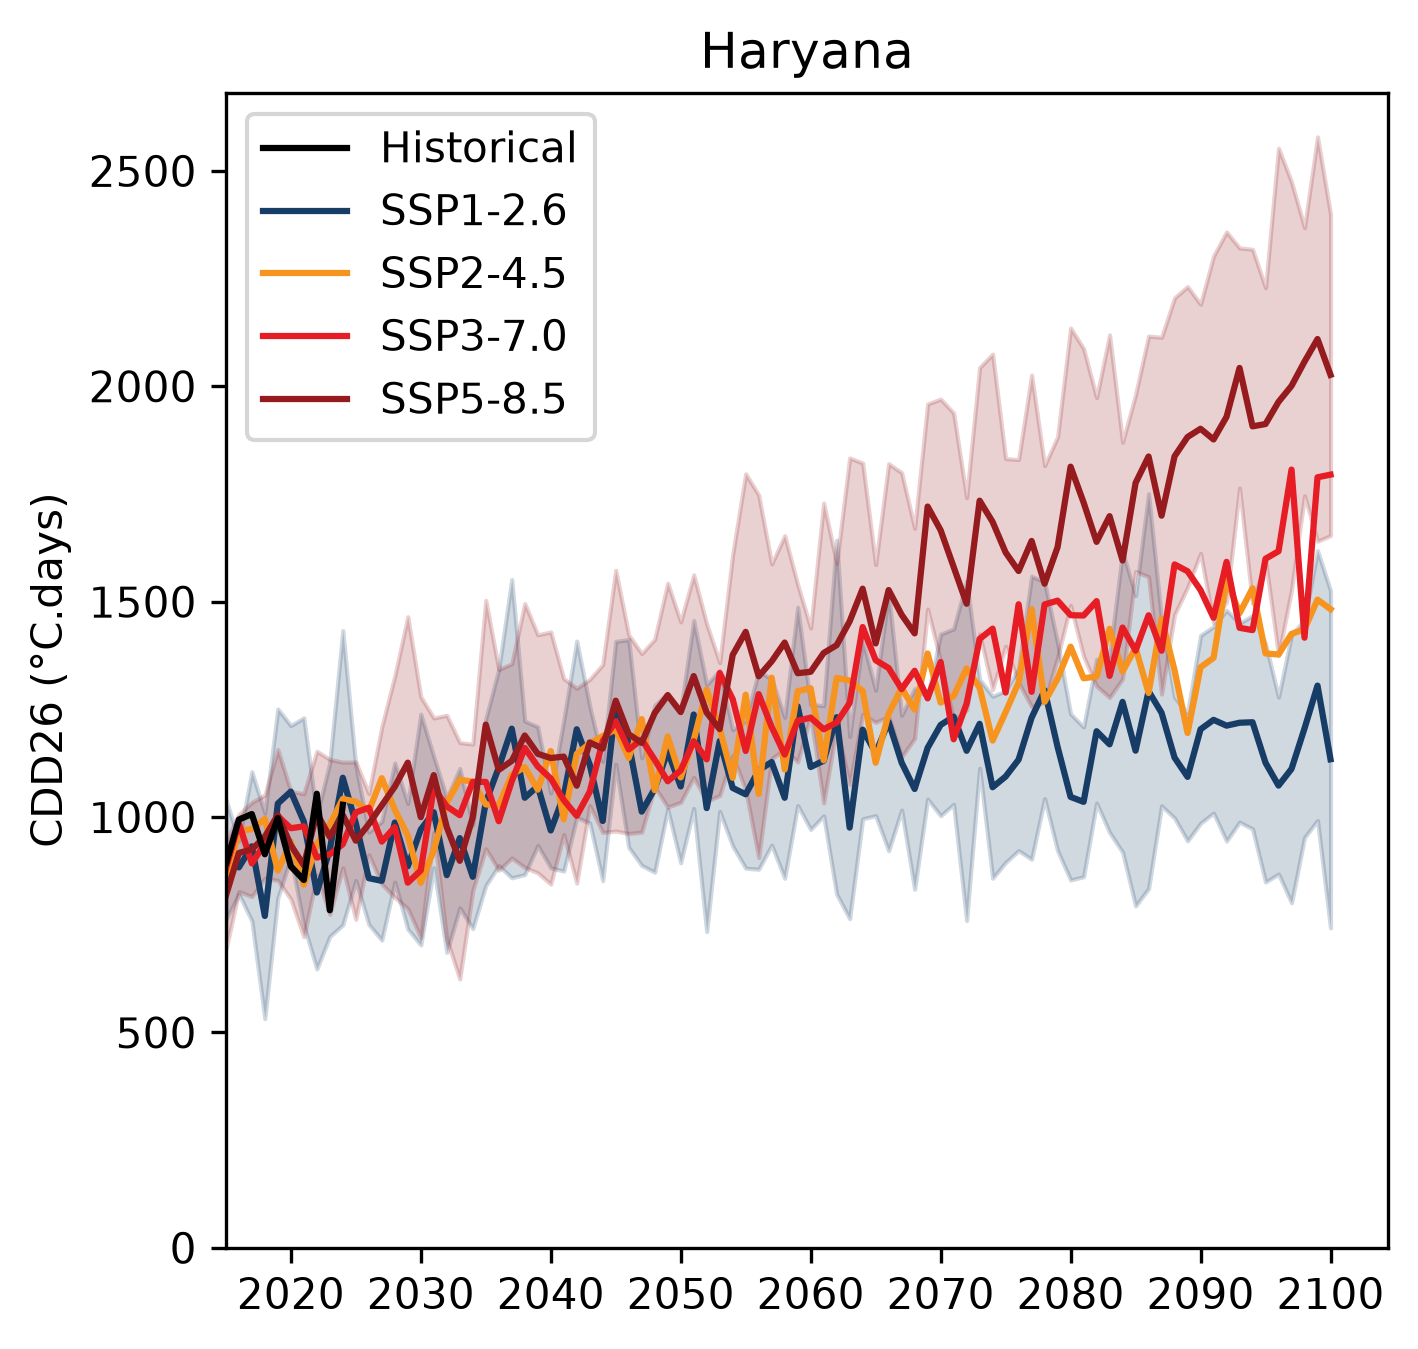
\includegraphics[height=0.25\textheight]{figures/projection_states/projection_cdd26_Haryana.png}\hfill
   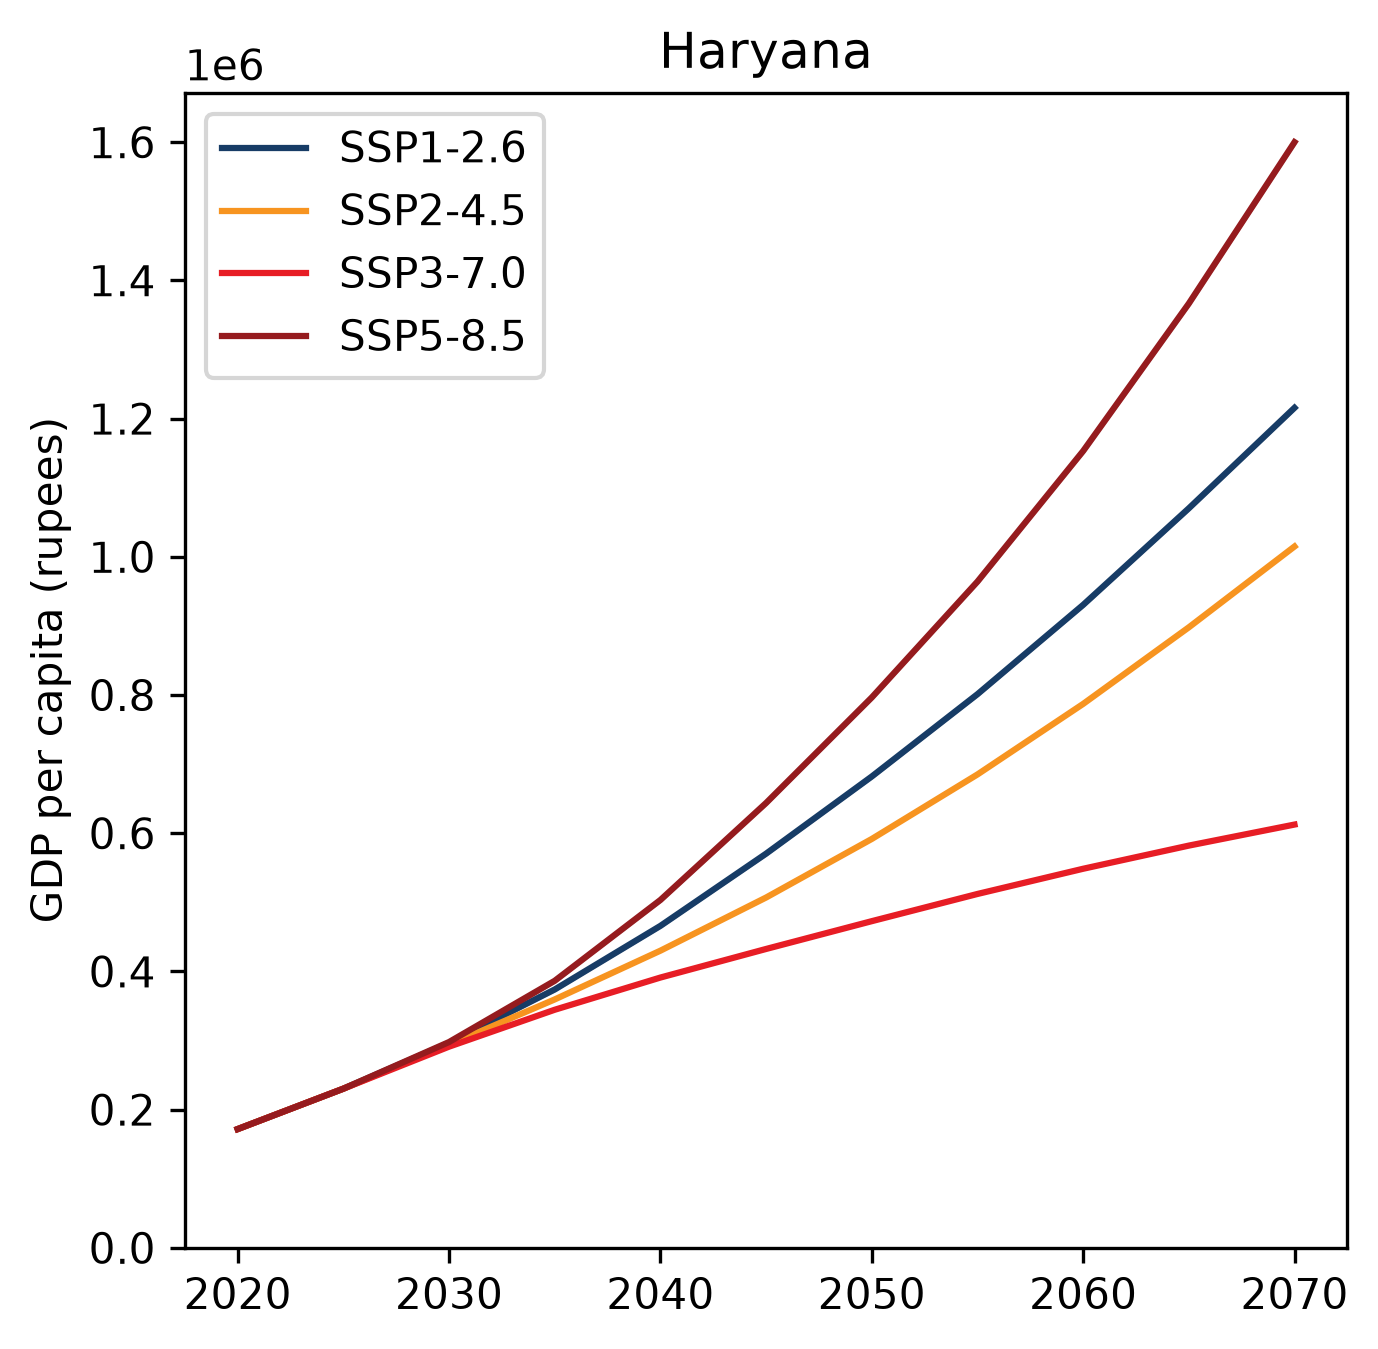
\includegraphics[height=0.25\textheight]{figures/projection_states/projection_gdp_per_capita_Haryana.png}\\
   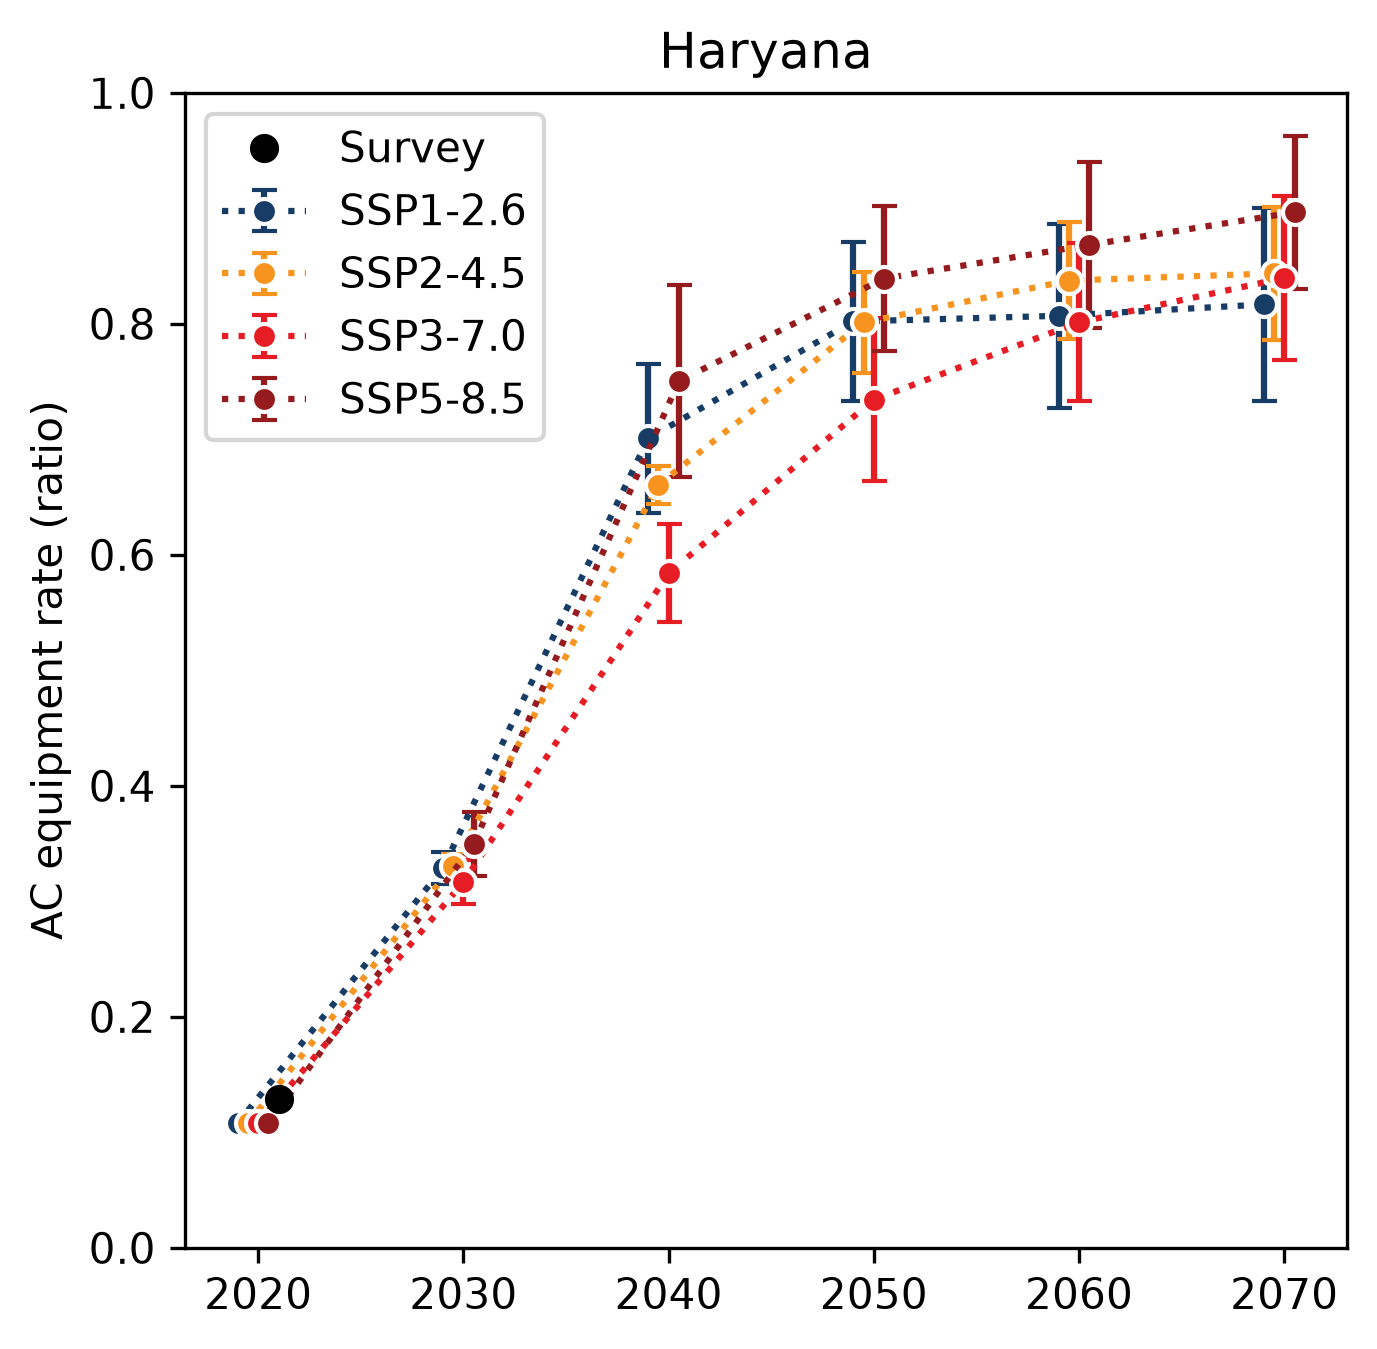
\includegraphics[height=0.25\textheight]{figures/projection_states/projection_ac_rate_Haryana.png}\hfill
   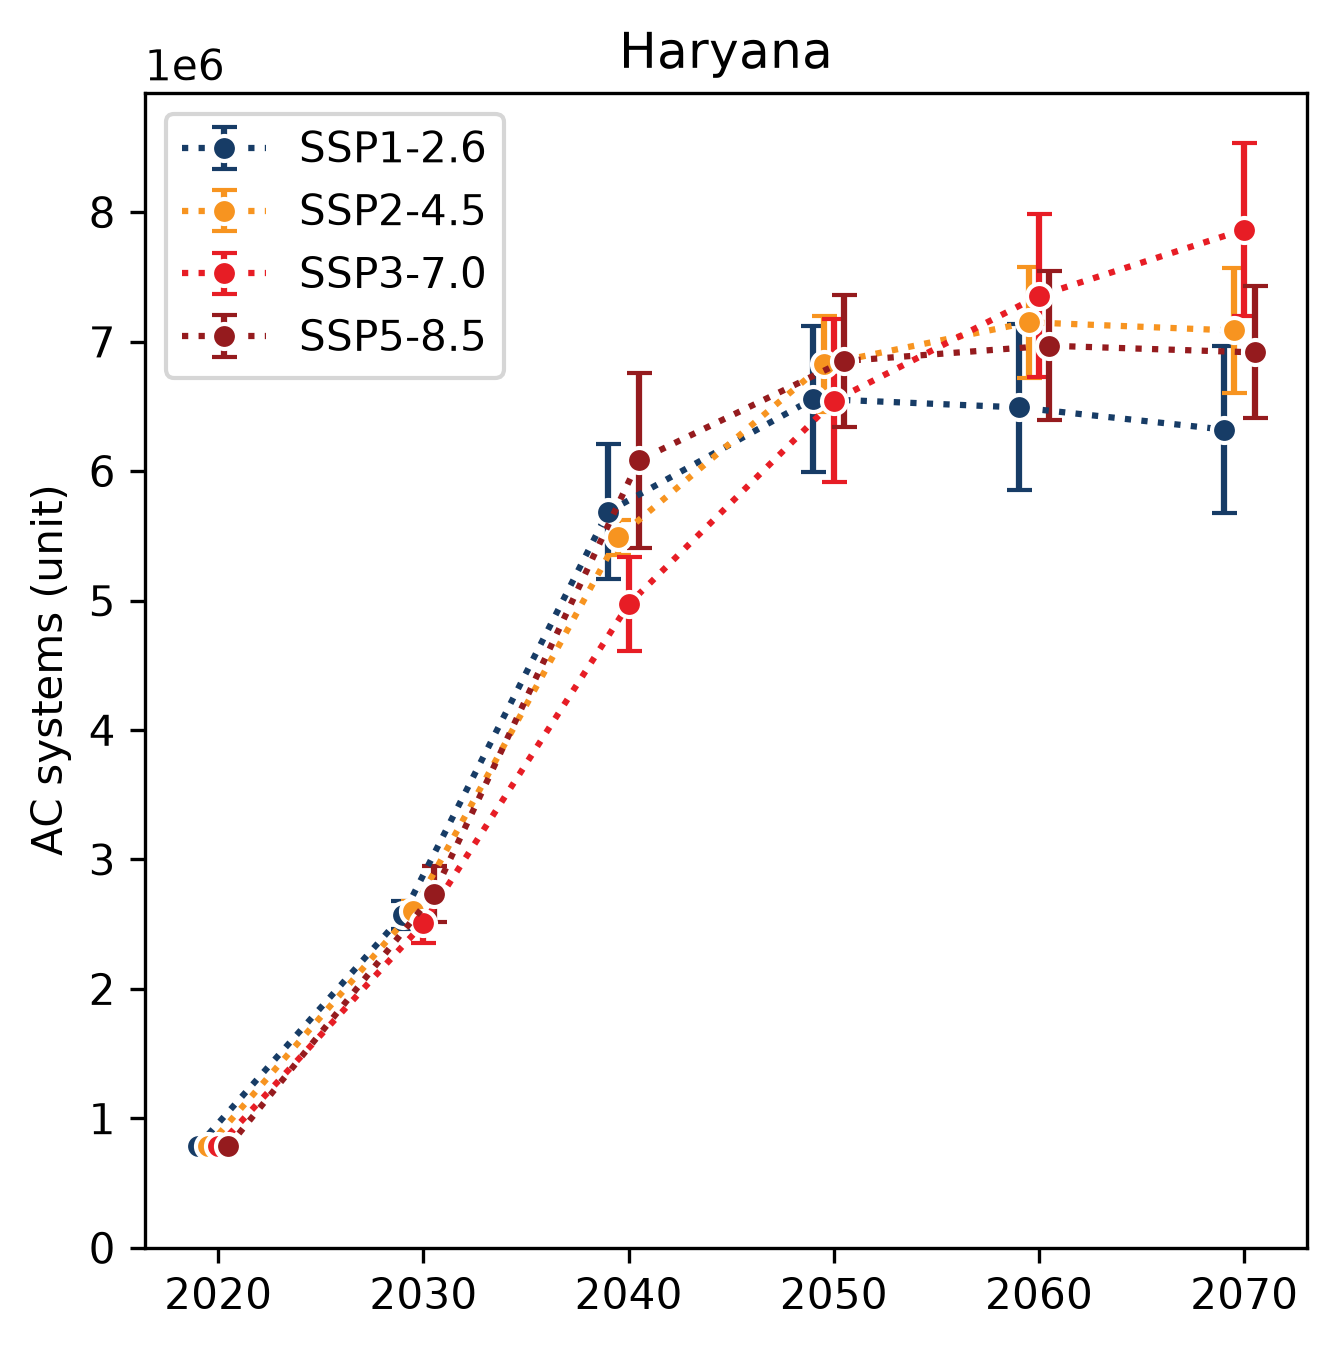
\includegraphics[height=0.25\textheight]{figures/projection_states/projection_ac_systems_Haryana.png}
   \caption{Projections des différentes variables pour Haryana}
\end{figure}

\clearpage

\subsubsection{Himachal Pradesh}

\begin{figure}[ht]
   \centering
   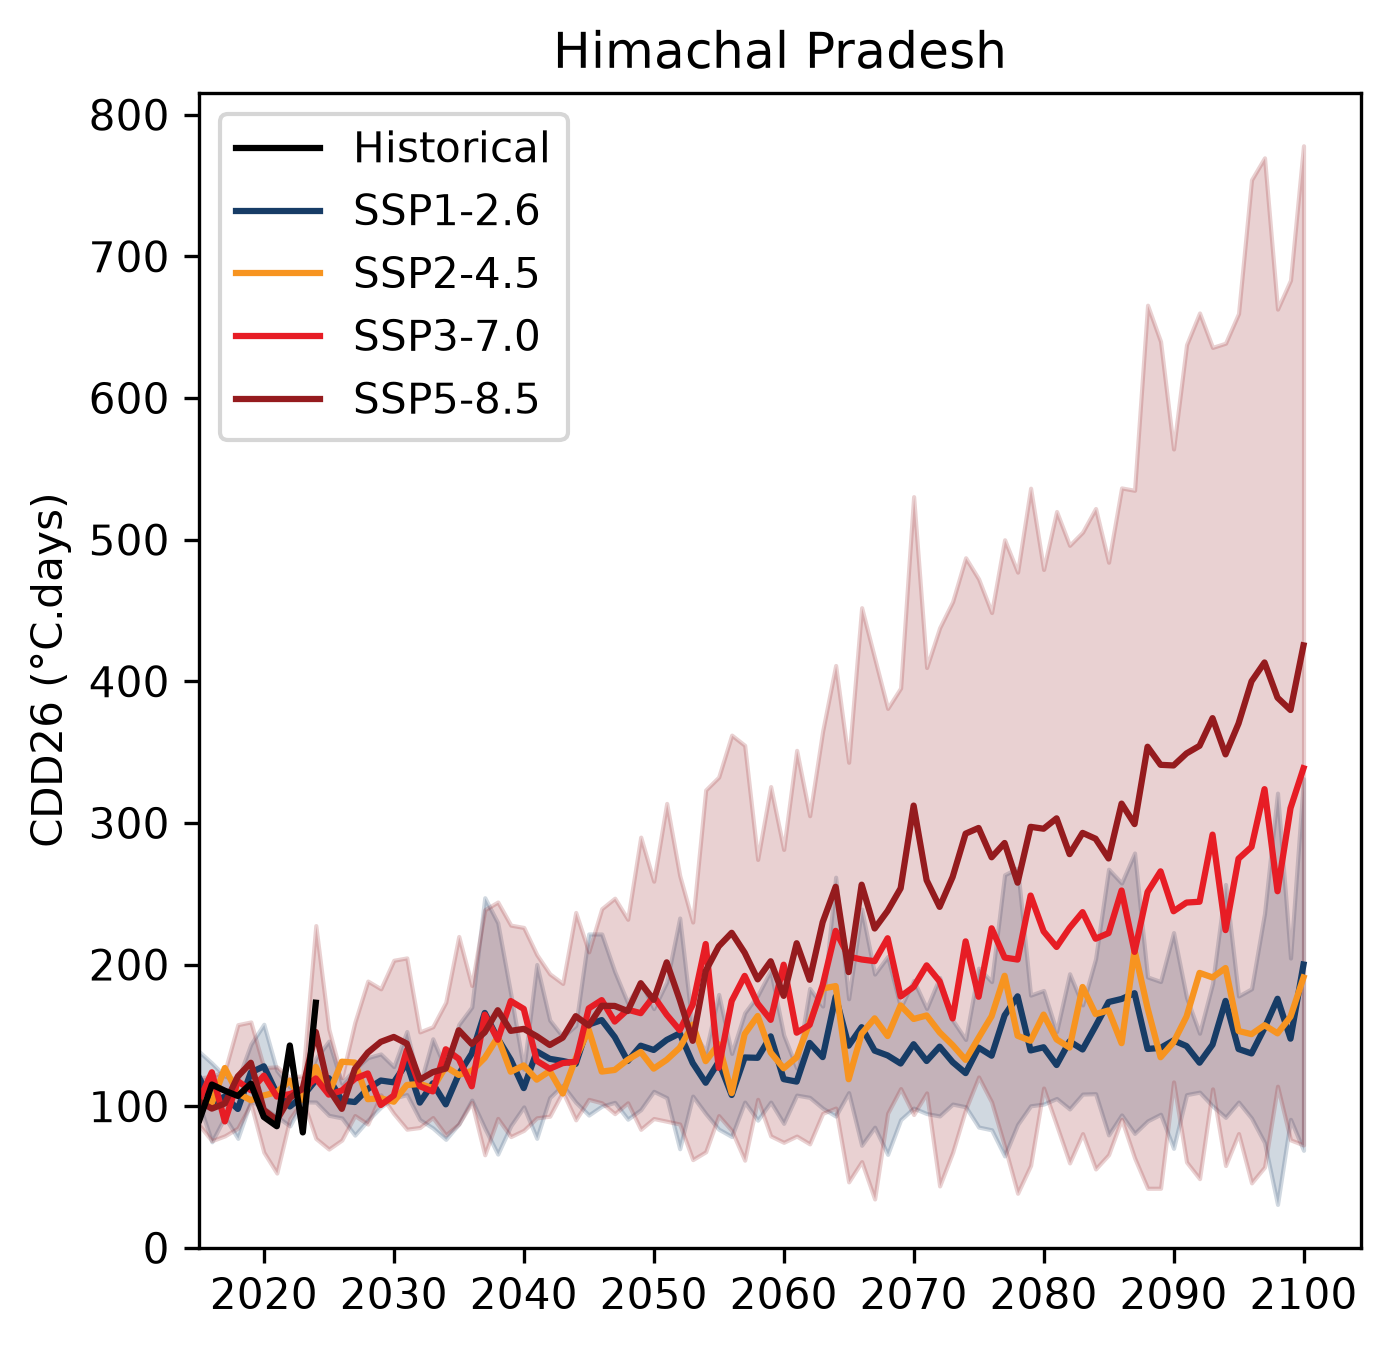
\includegraphics[height=0.25\textheight]{figures/projection_states/projection_cdd26_Himachal Pradesh.png}\hfill
   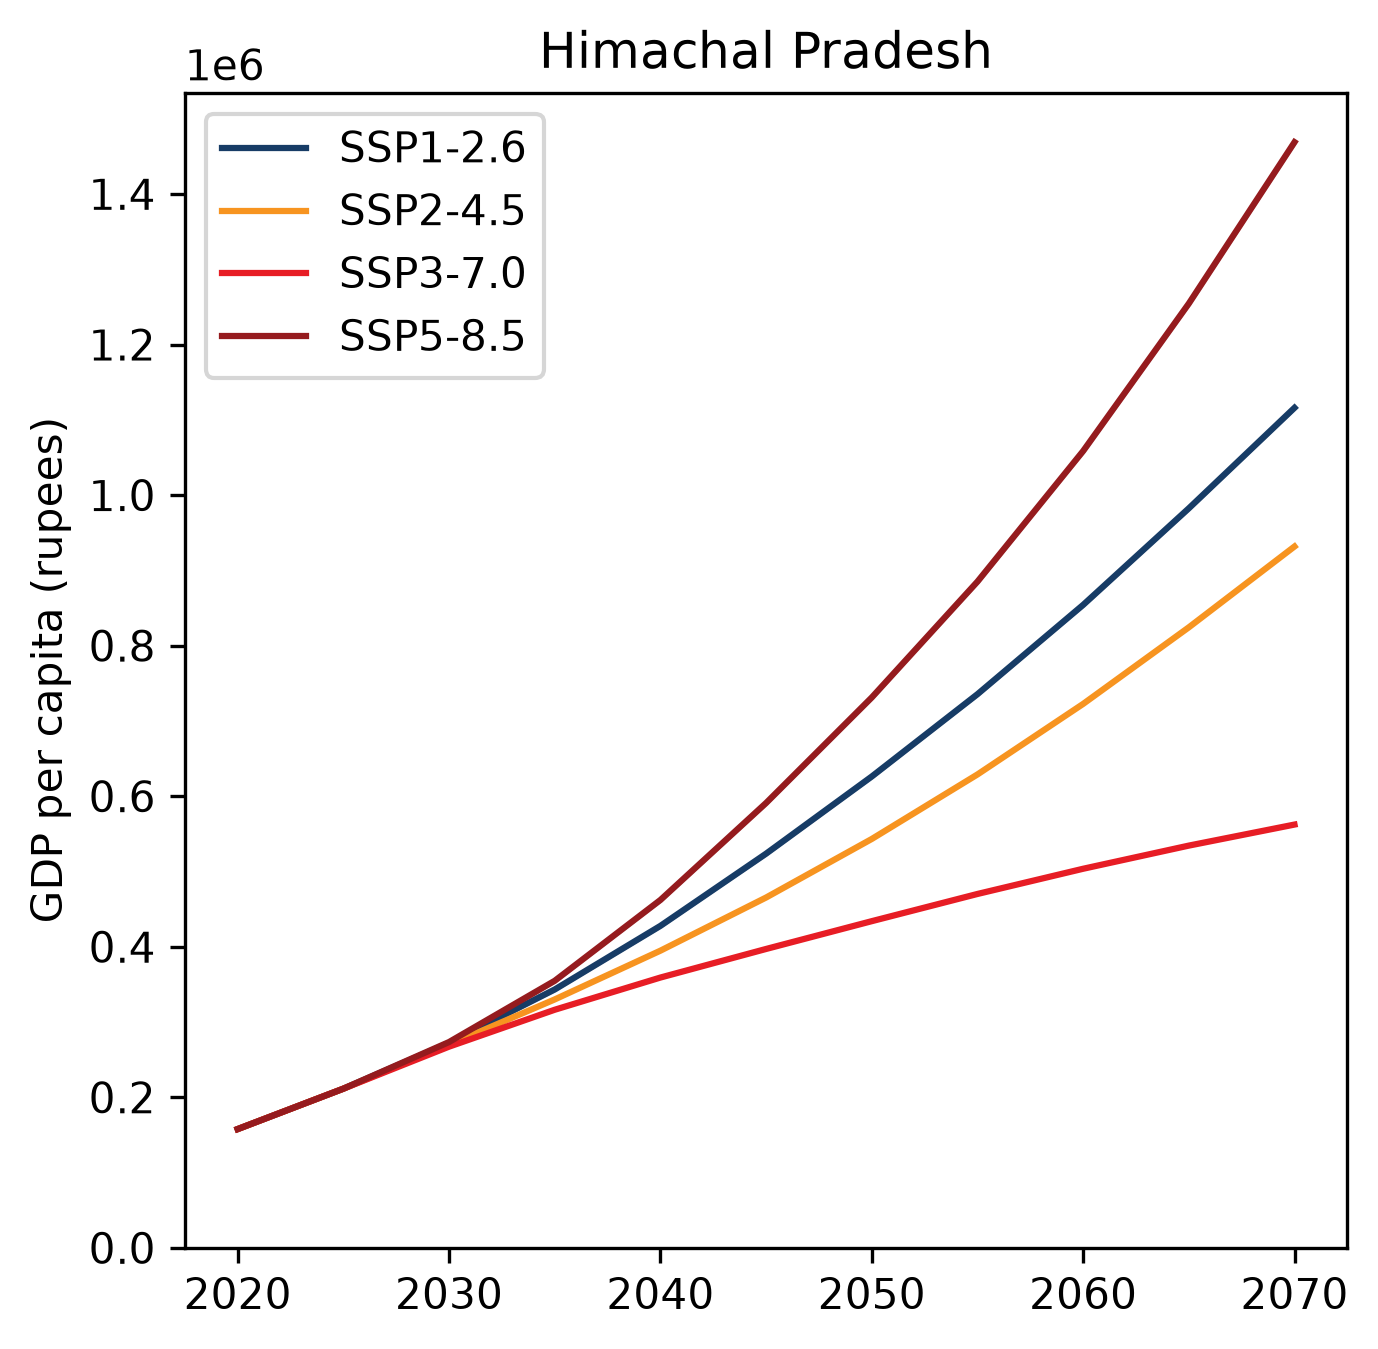
\includegraphics[height=0.25\textheight]{figures/projection_states/projection_gdp_per_capita_Himachal Pradesh.png}\\
   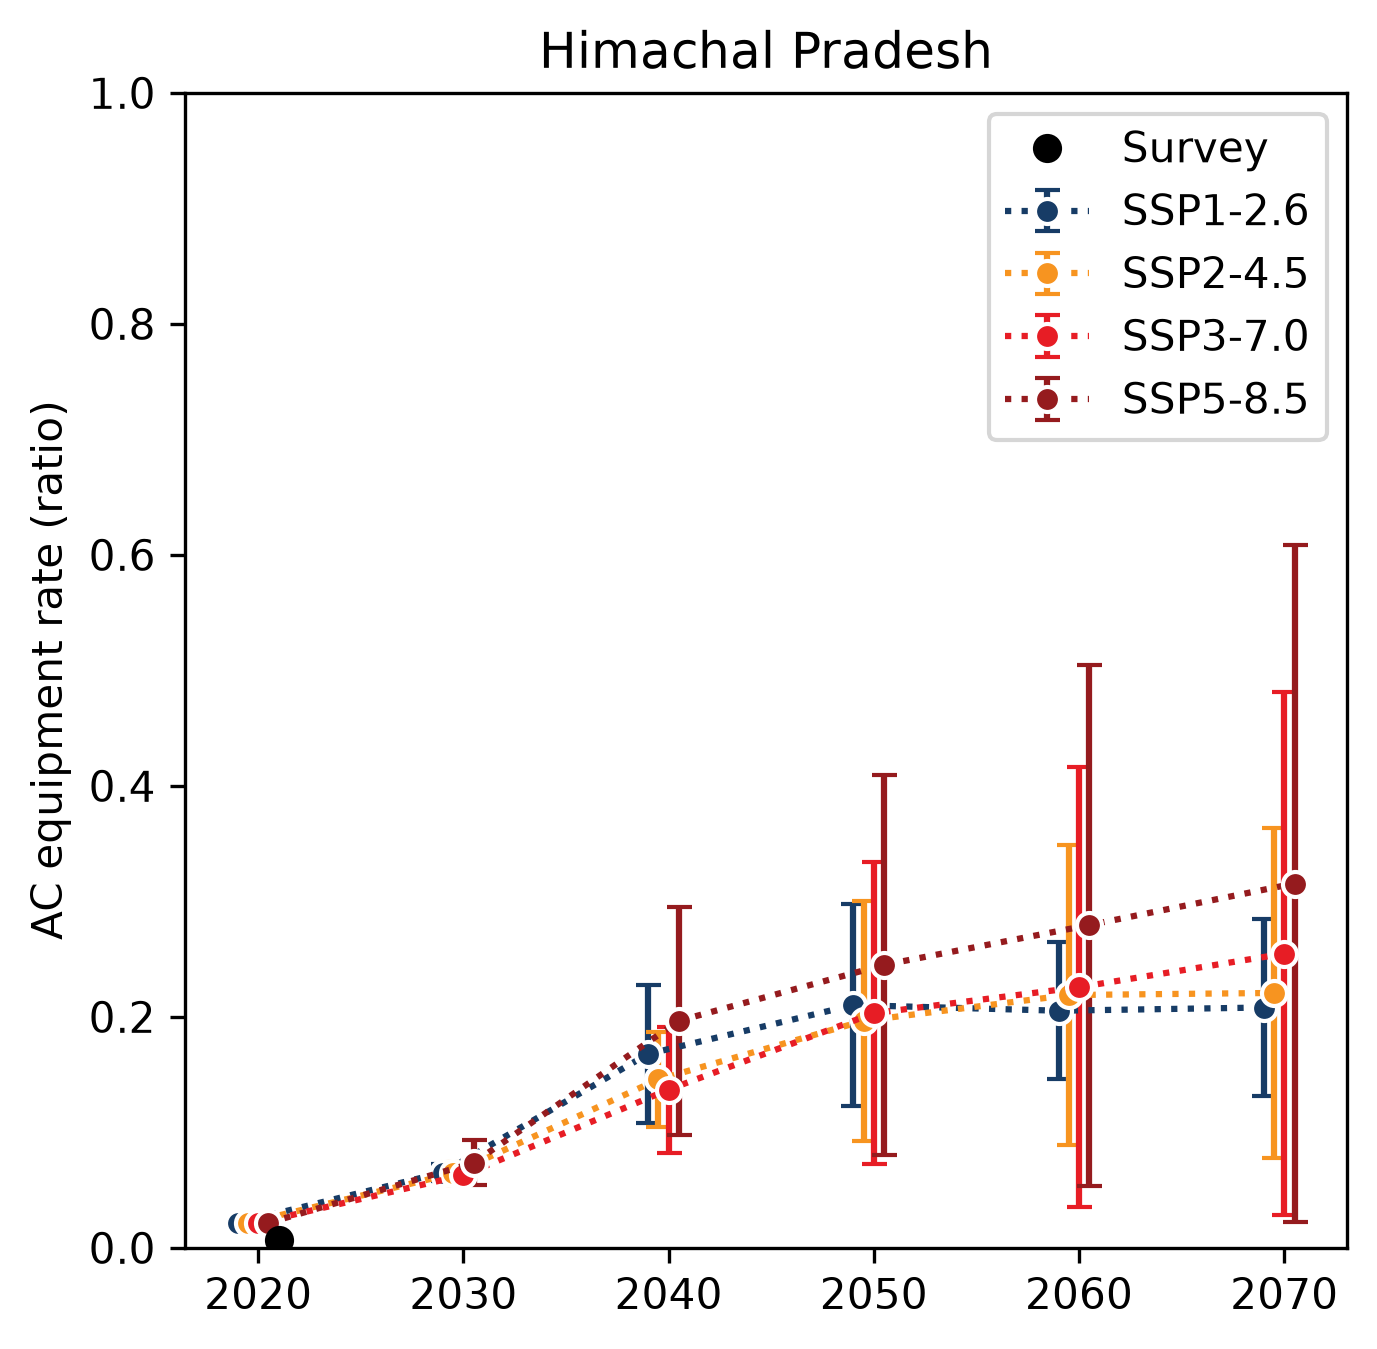
\includegraphics[height=0.25\textheight]{figures/projection_states/projection_ac_rate_Himachal Pradesh.png}\hfill
   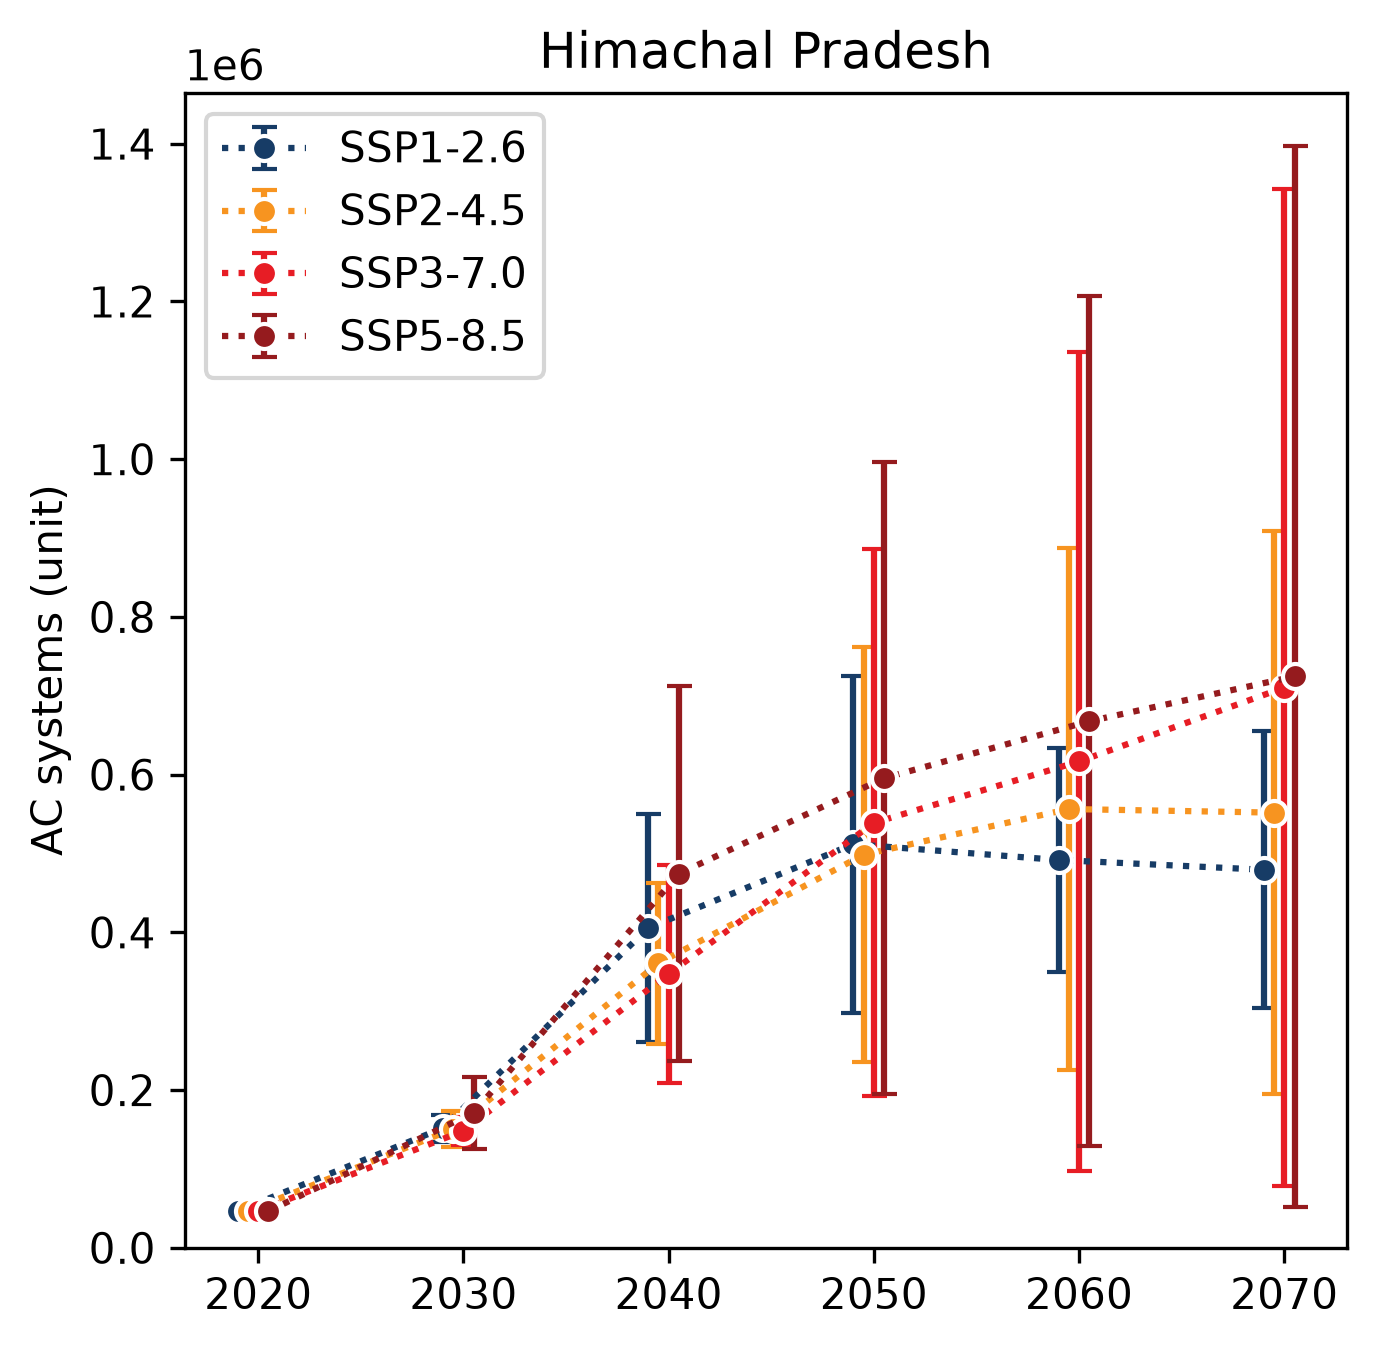
\includegraphics[height=0.25\textheight]{figures/projection_states/projection_ac_systems_Himachal Pradesh.png}
   \caption{Projections des différentes variables pour Himachal Pradesh}
\end{figure}

\clearpage

\subsubsection{Jharkhand}

\begin{figure}[ht]
   \centering
   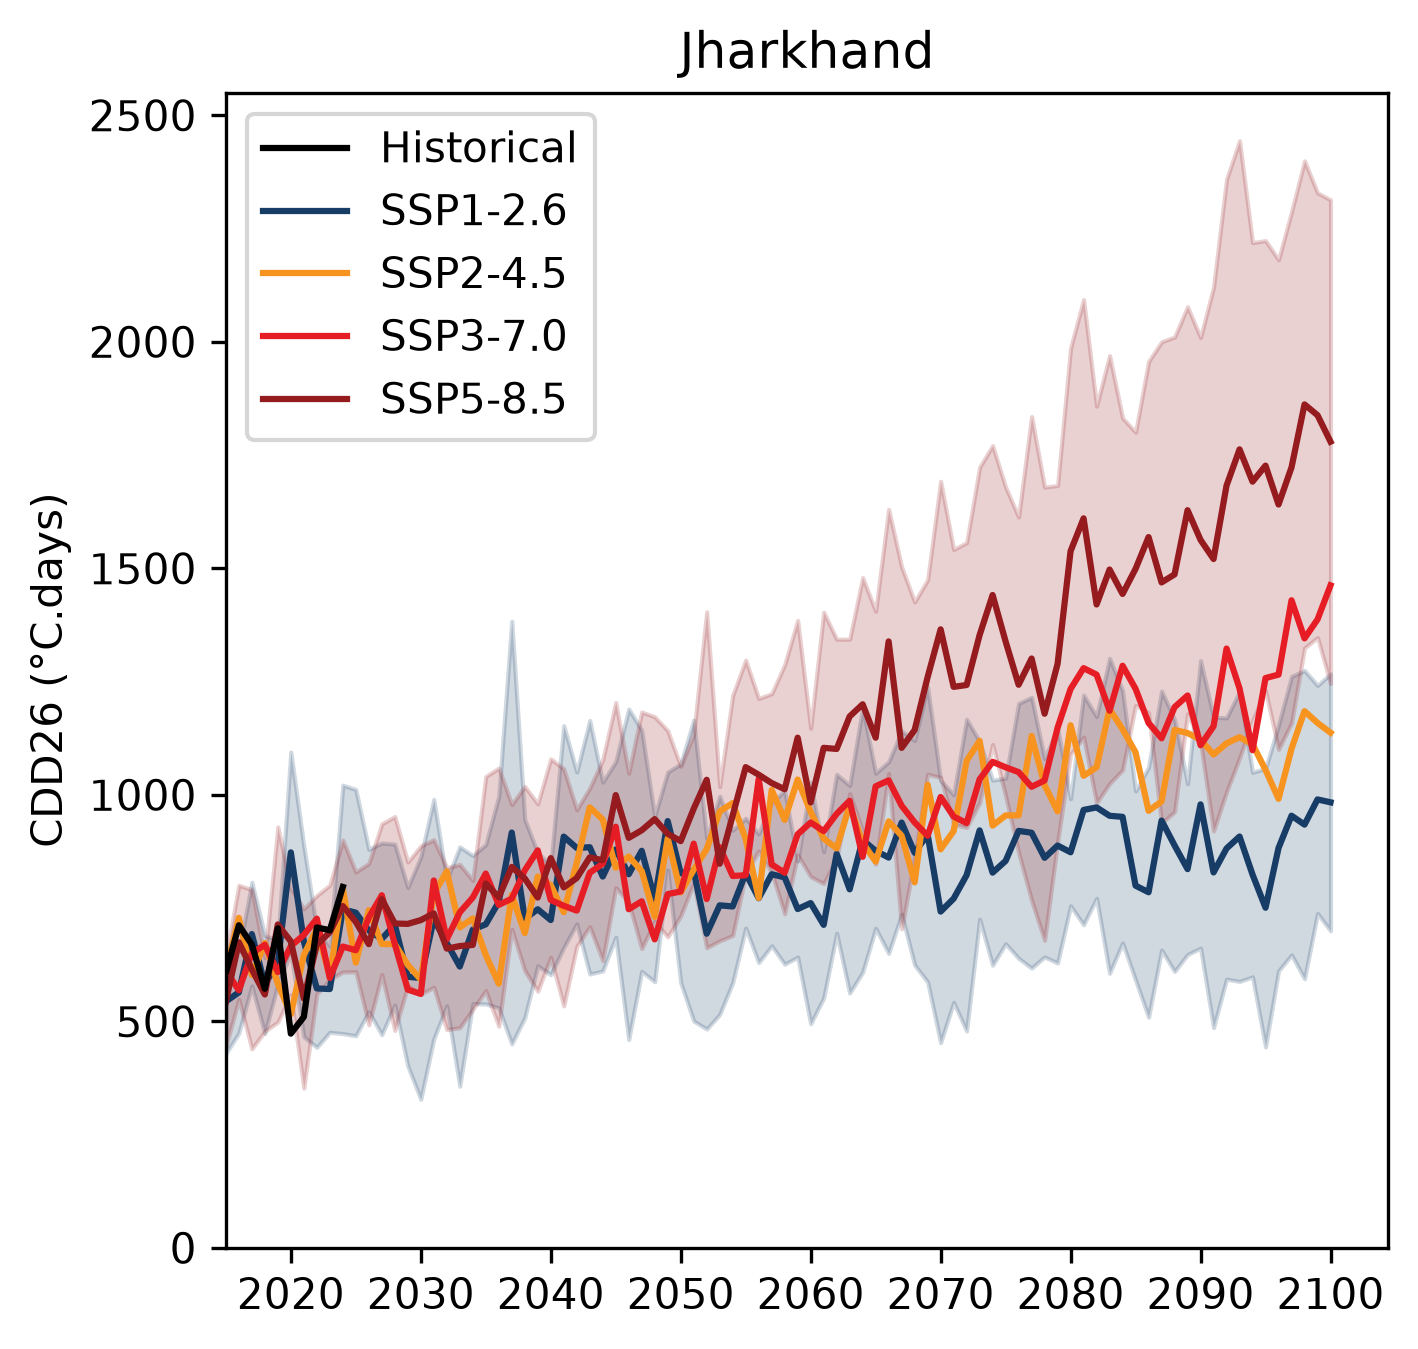
\includegraphics[height=0.25\textheight]{figures/projection_states/projection_cdd26_Jharkhand.png}\hfill
   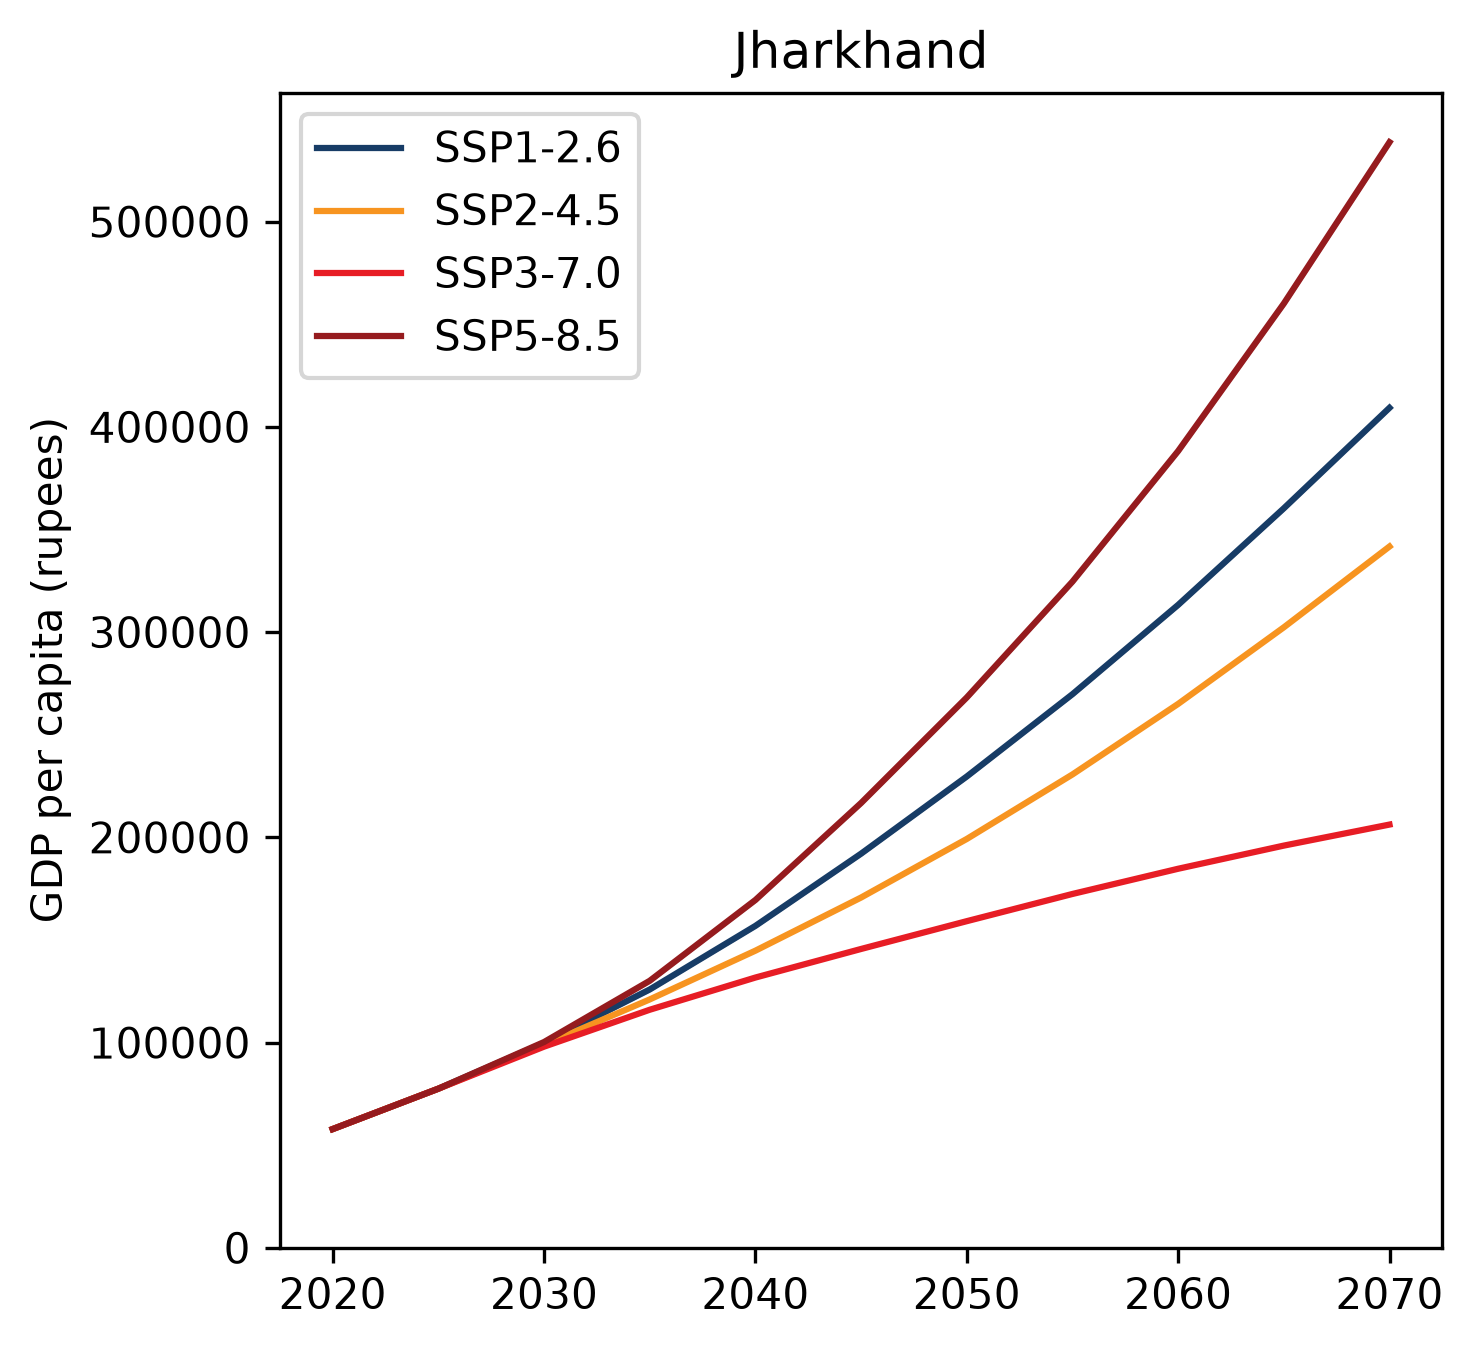
\includegraphics[height=0.25\textheight]{figures/projection_states/projection_gdp_per_capita_Jharkhand.png}\\
   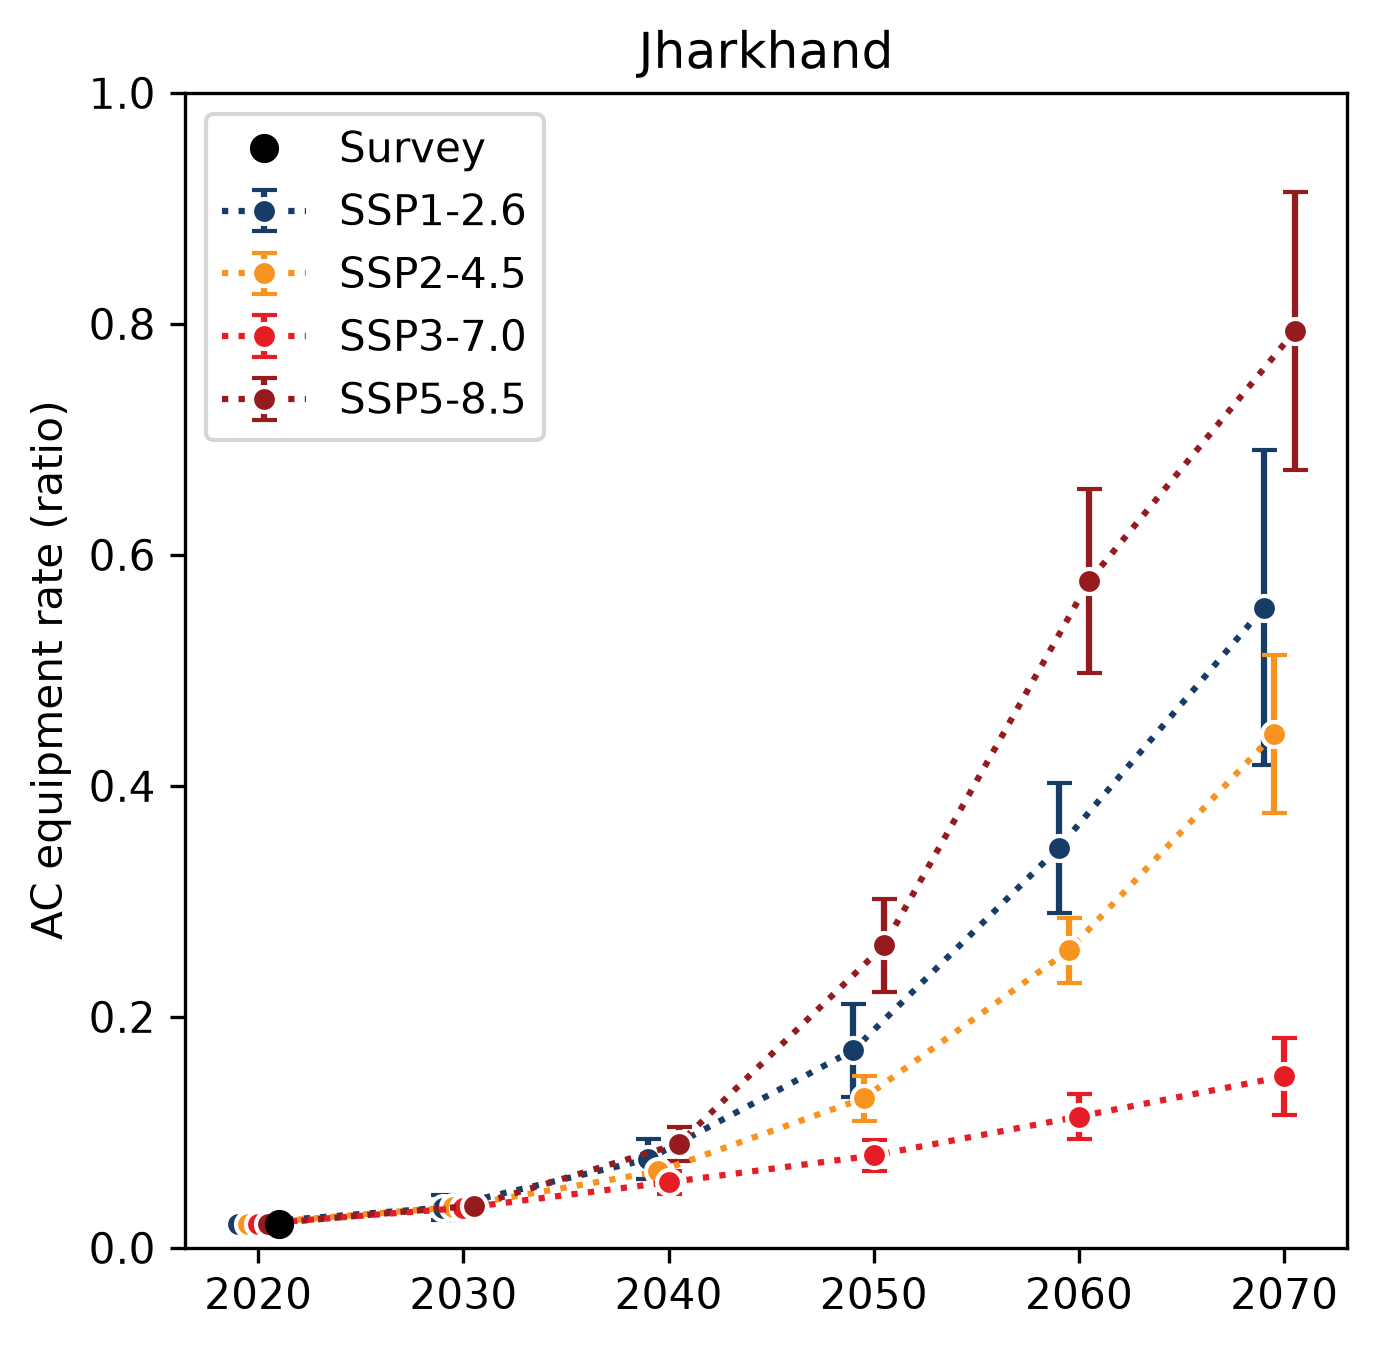
\includegraphics[height=0.25\textheight]{figures/projection_states/projection_ac_rate_Jharkhand.png}\hfill
   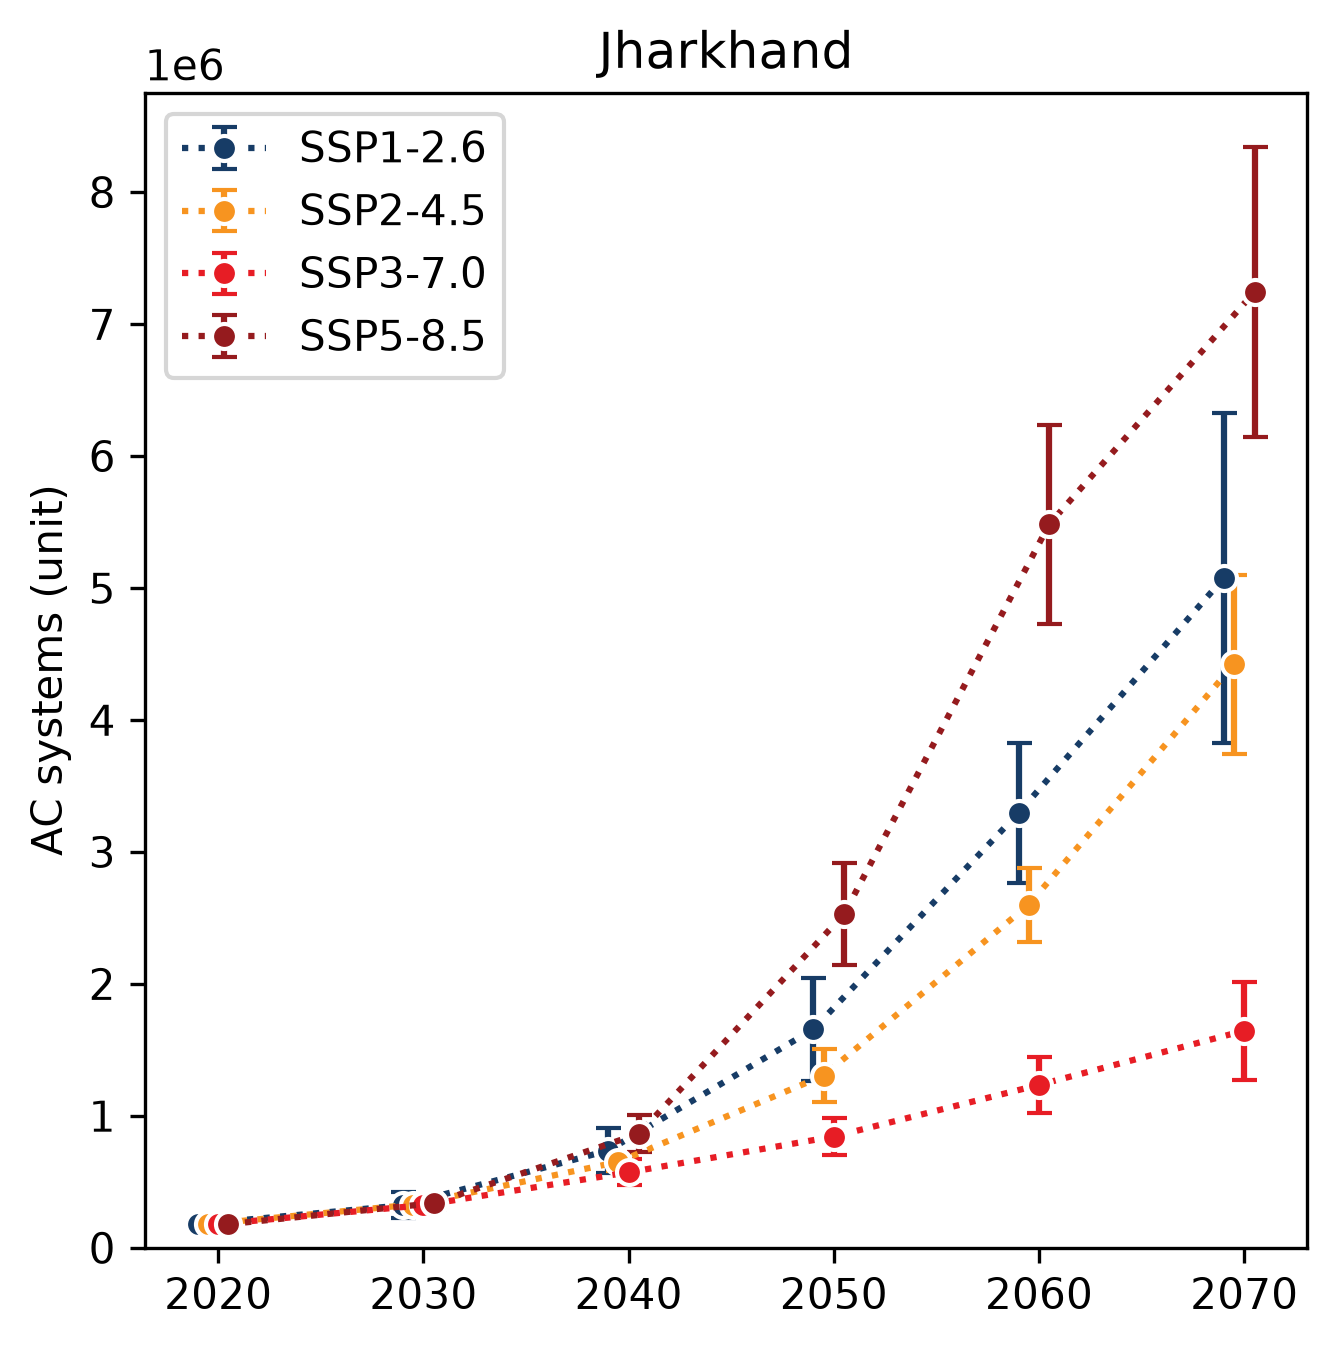
\includegraphics[height=0.25\textheight]{figures/projection_states/projection_ac_systems_Jharkhand.png}
   \caption{Projections des différentes variables pour Jharkhand}
\end{figure}

\clearpage

\subsubsection{Karnataka}

\begin{figure}[ht]
   \centering
   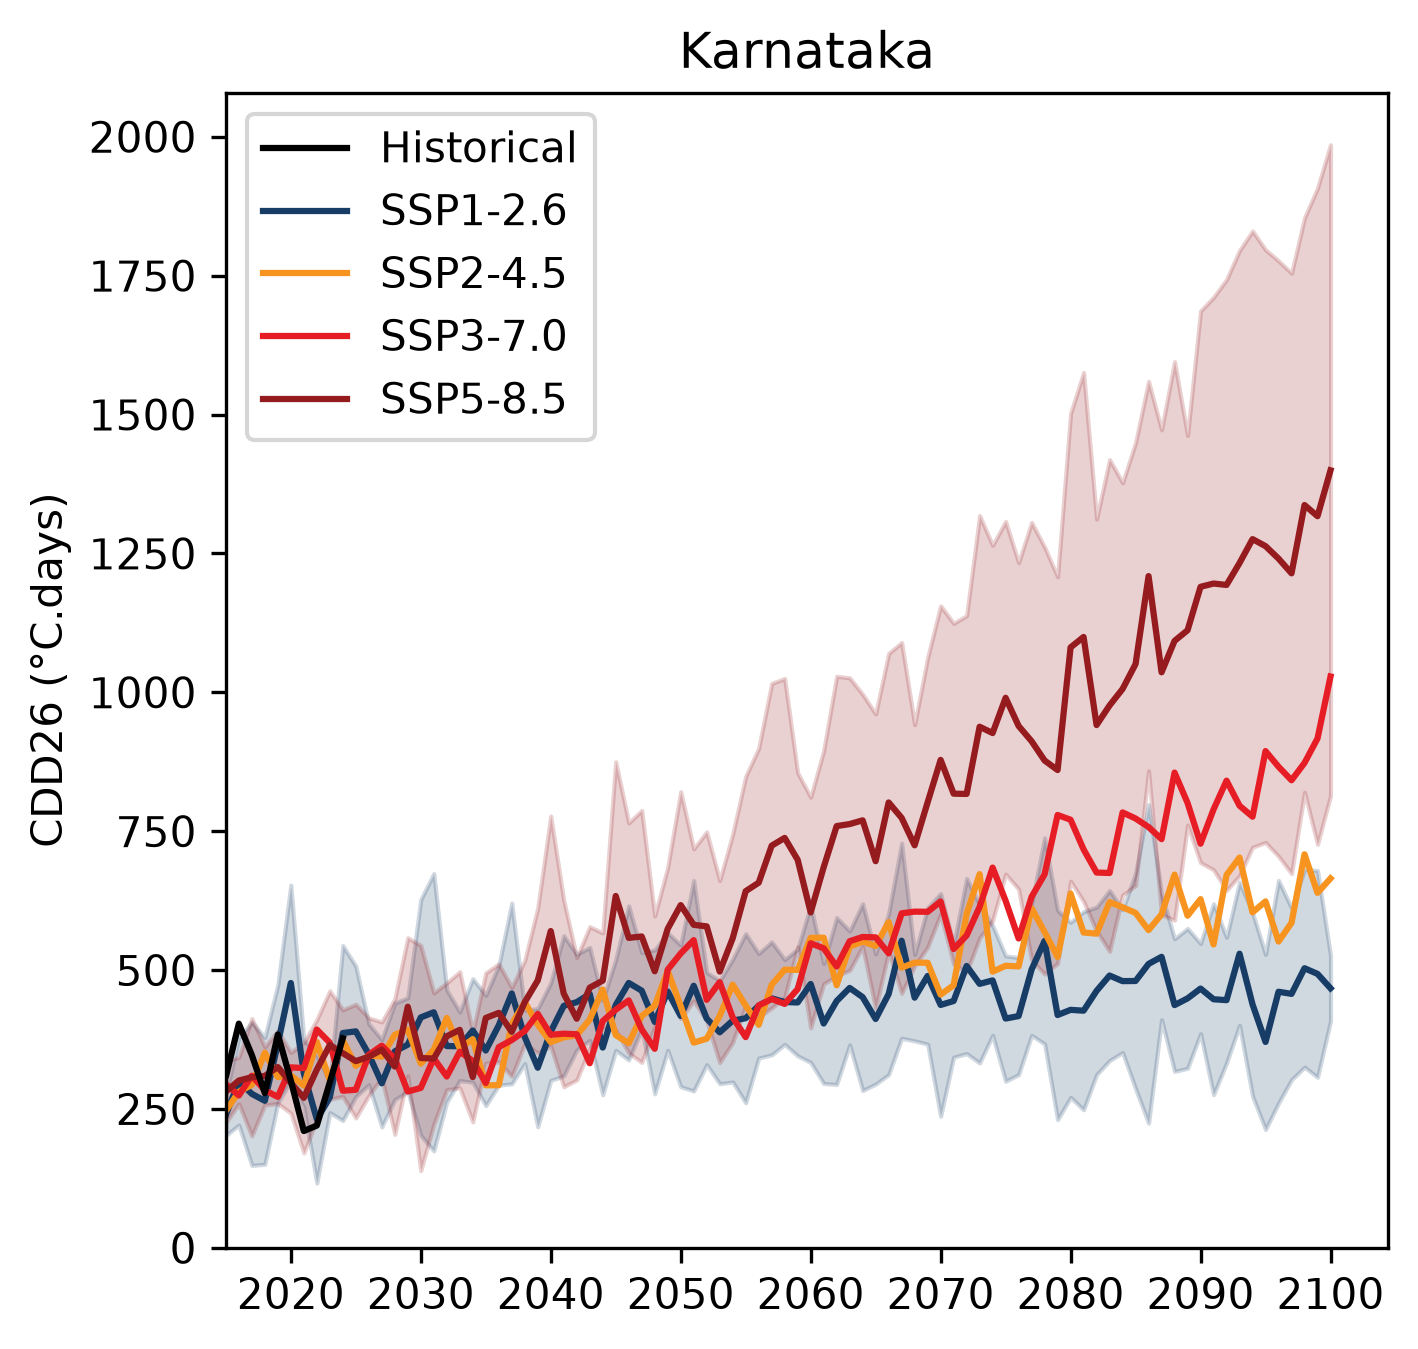
\includegraphics[height=0.25\textheight]{figures/projection_states/projection_cdd26_Karnataka.png}\hfill
   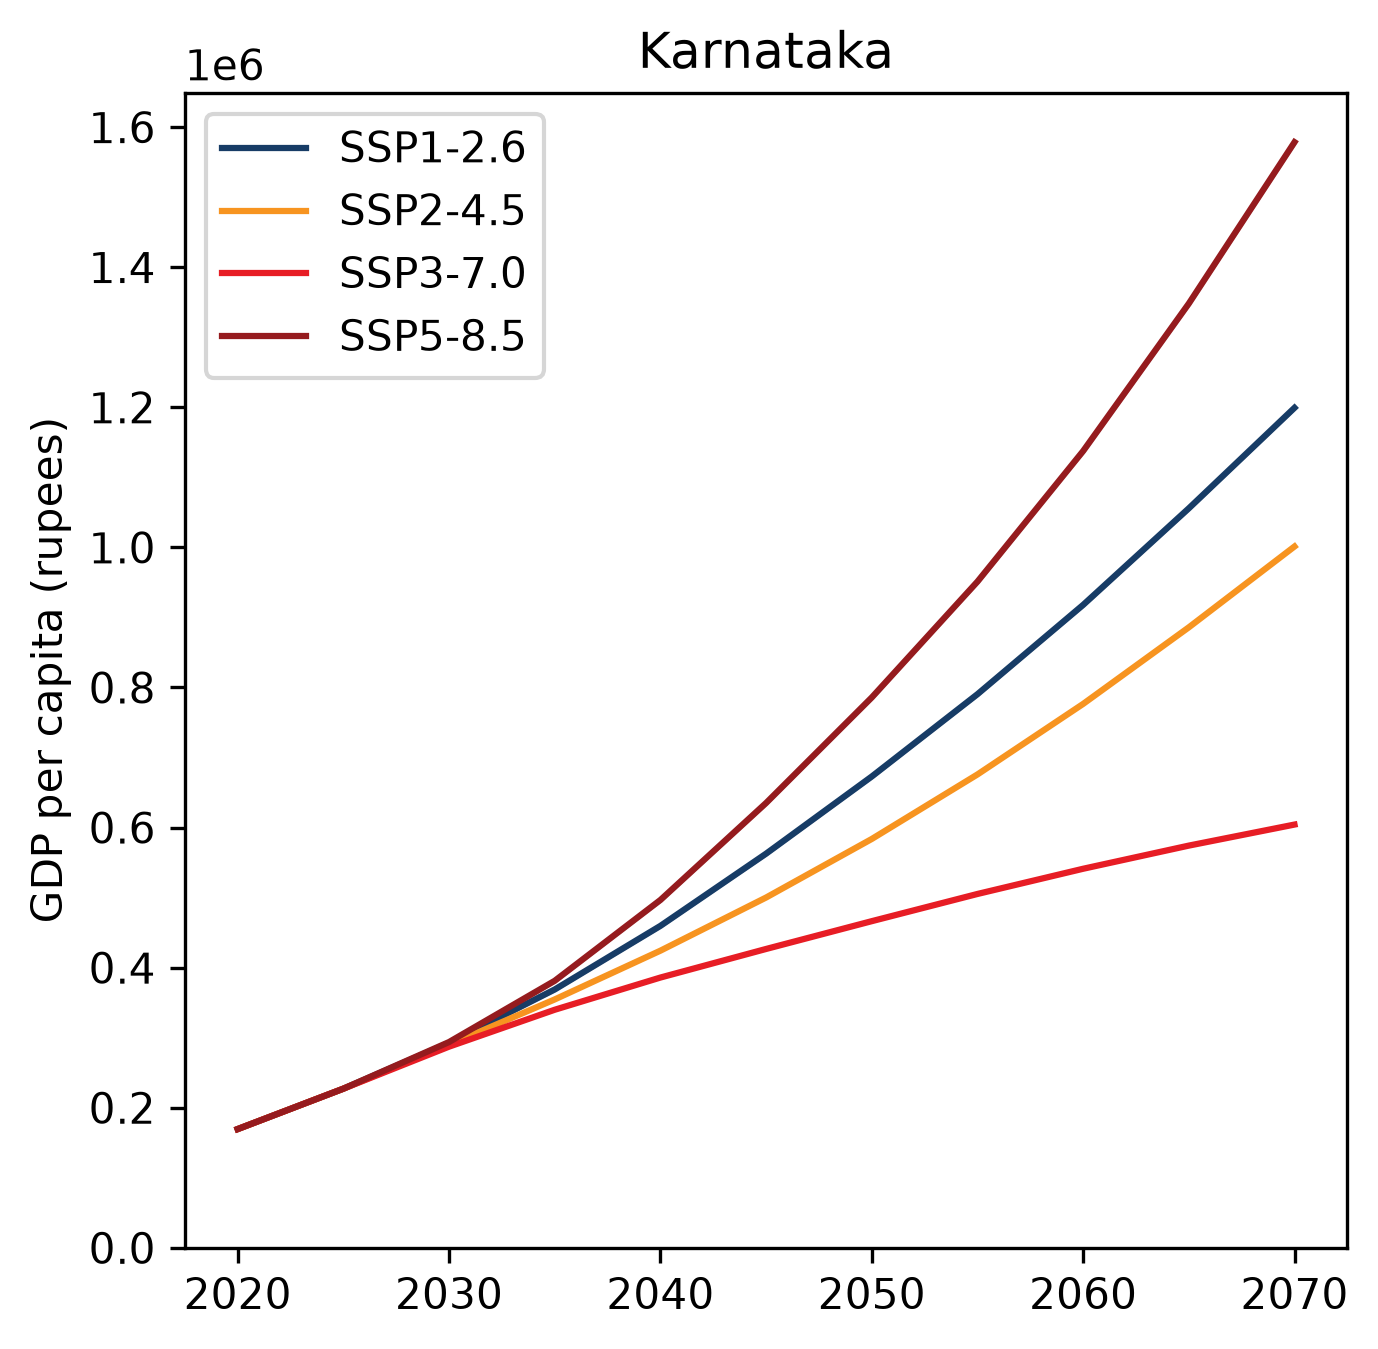
\includegraphics[height=0.25\textheight]{figures/projection_states/projection_gdp_per_capita_Karnataka.png}\\
   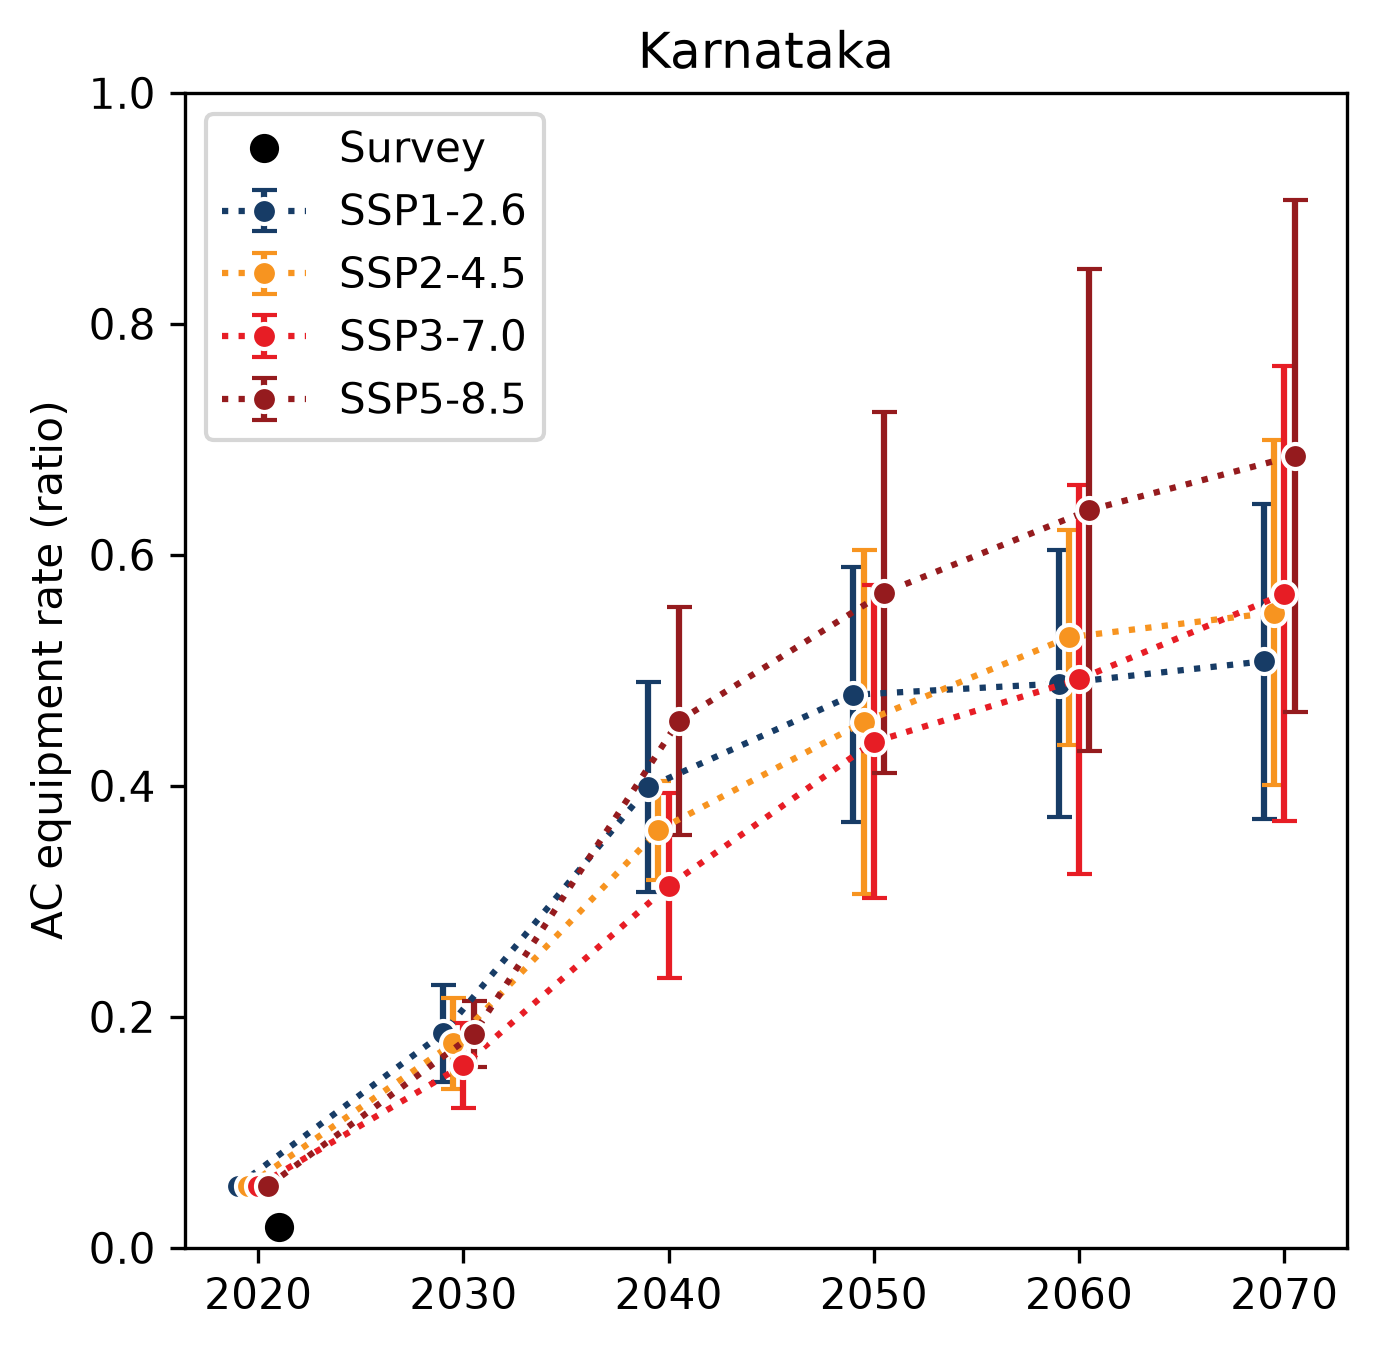
\includegraphics[height=0.25\textheight]{figures/projection_states/projection_ac_rate_Karnataka.png}\hfill
   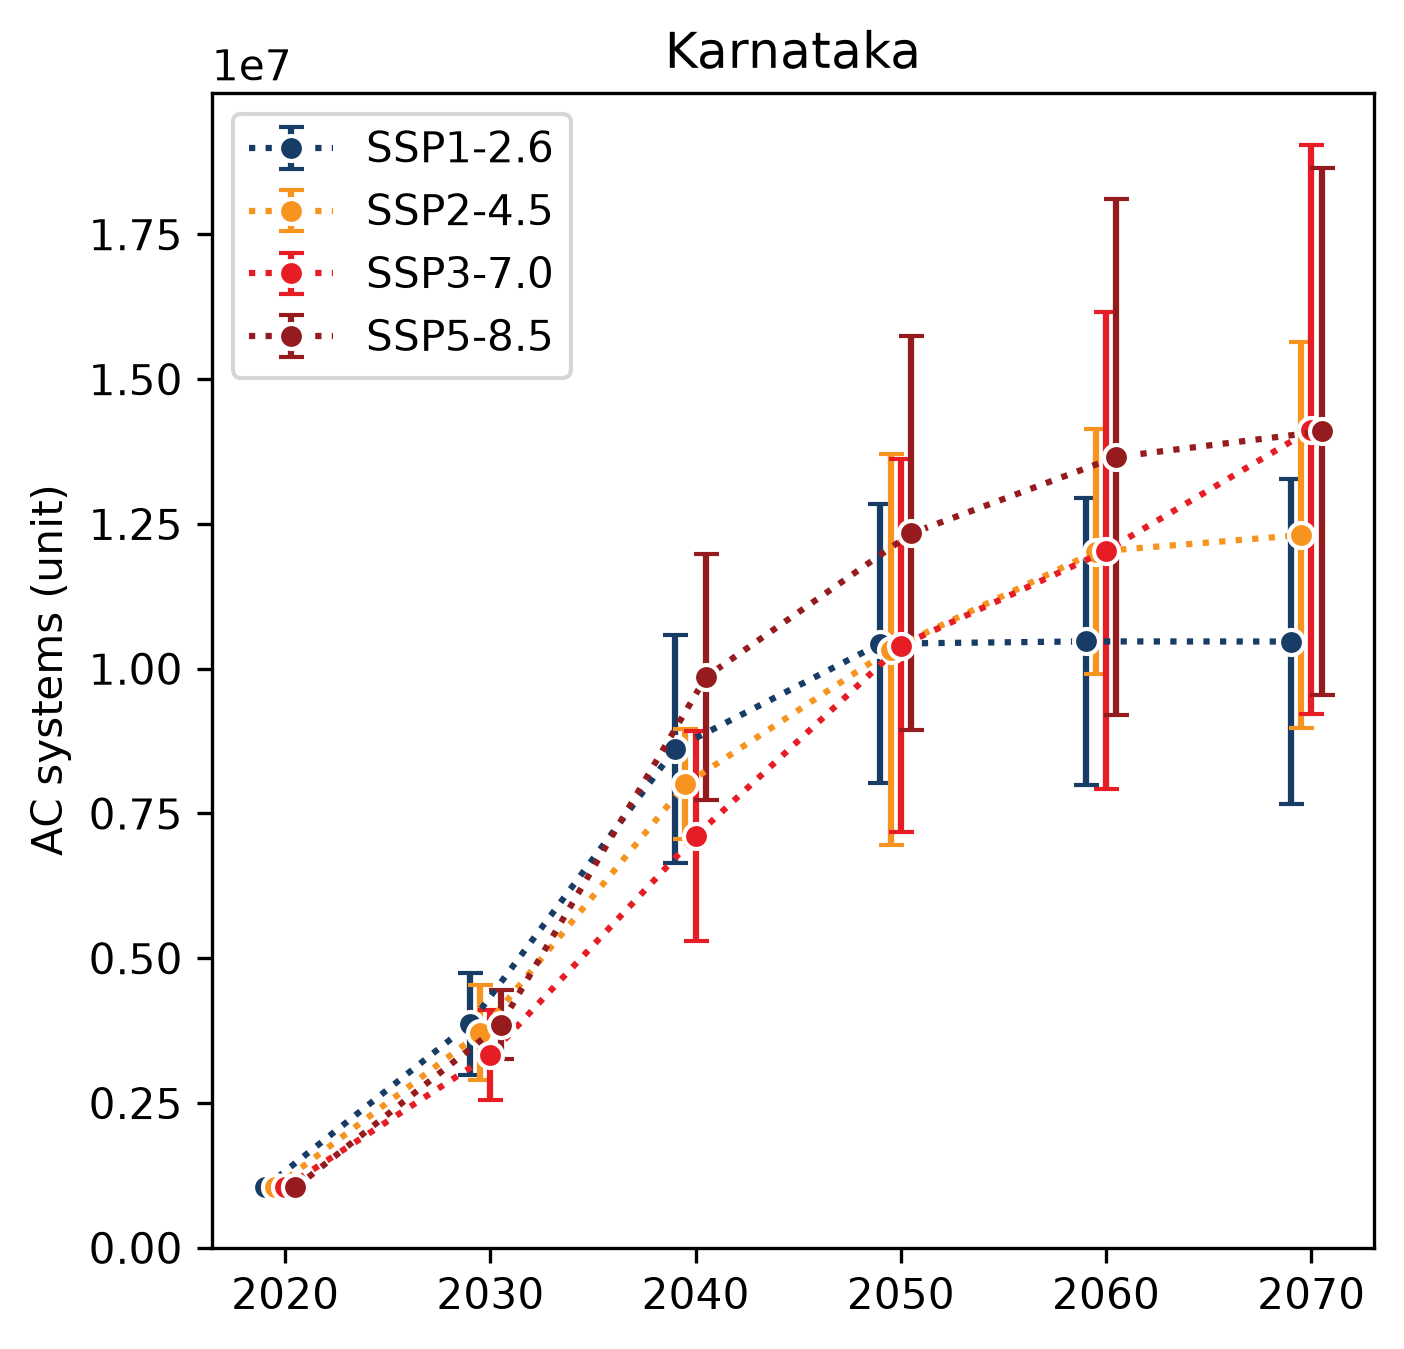
\includegraphics[height=0.25\textheight]{figures/projection_states/projection_ac_systems_Karnataka.png}
   \caption{Projections des différentes variables pour Karnataka}
\end{figure}

\clearpage

\subsubsection{Kerala}

\begin{figure}[ht]
   \centering
   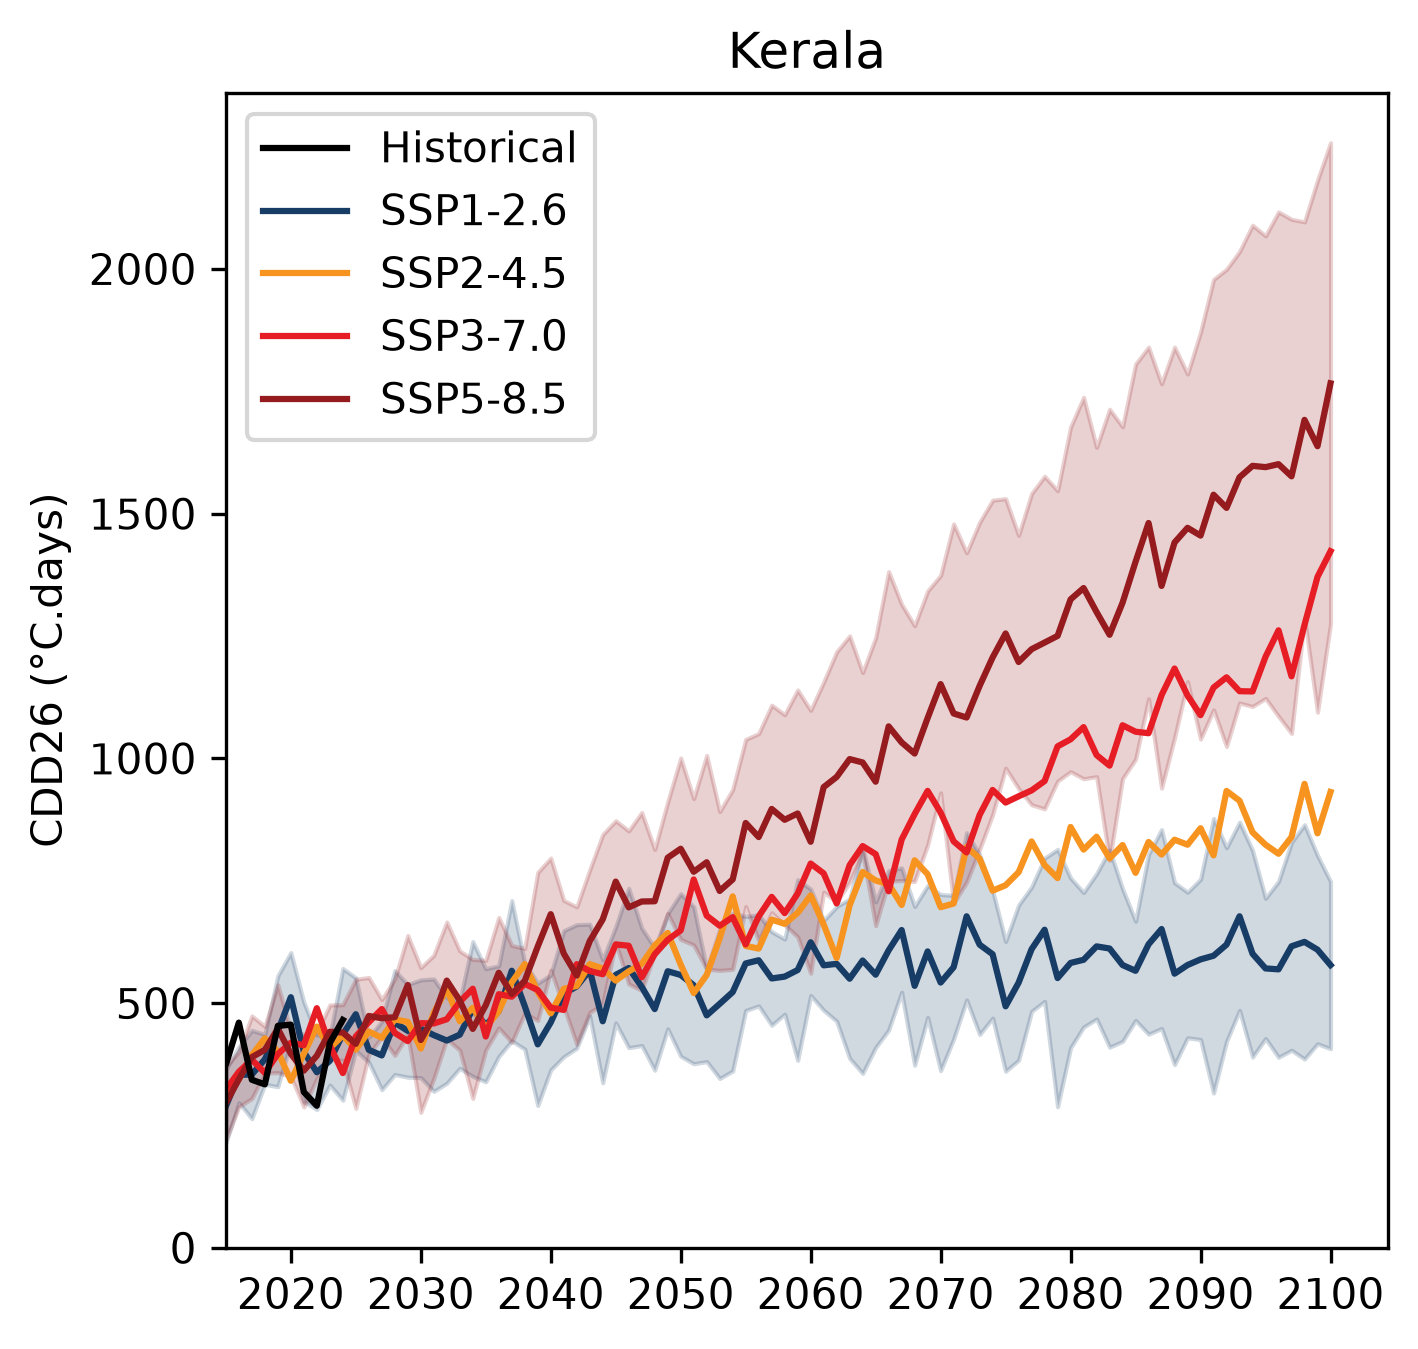
\includegraphics[height=0.25\textheight]{figures/projection_states/projection_cdd26_Kerala.png}\hfill
   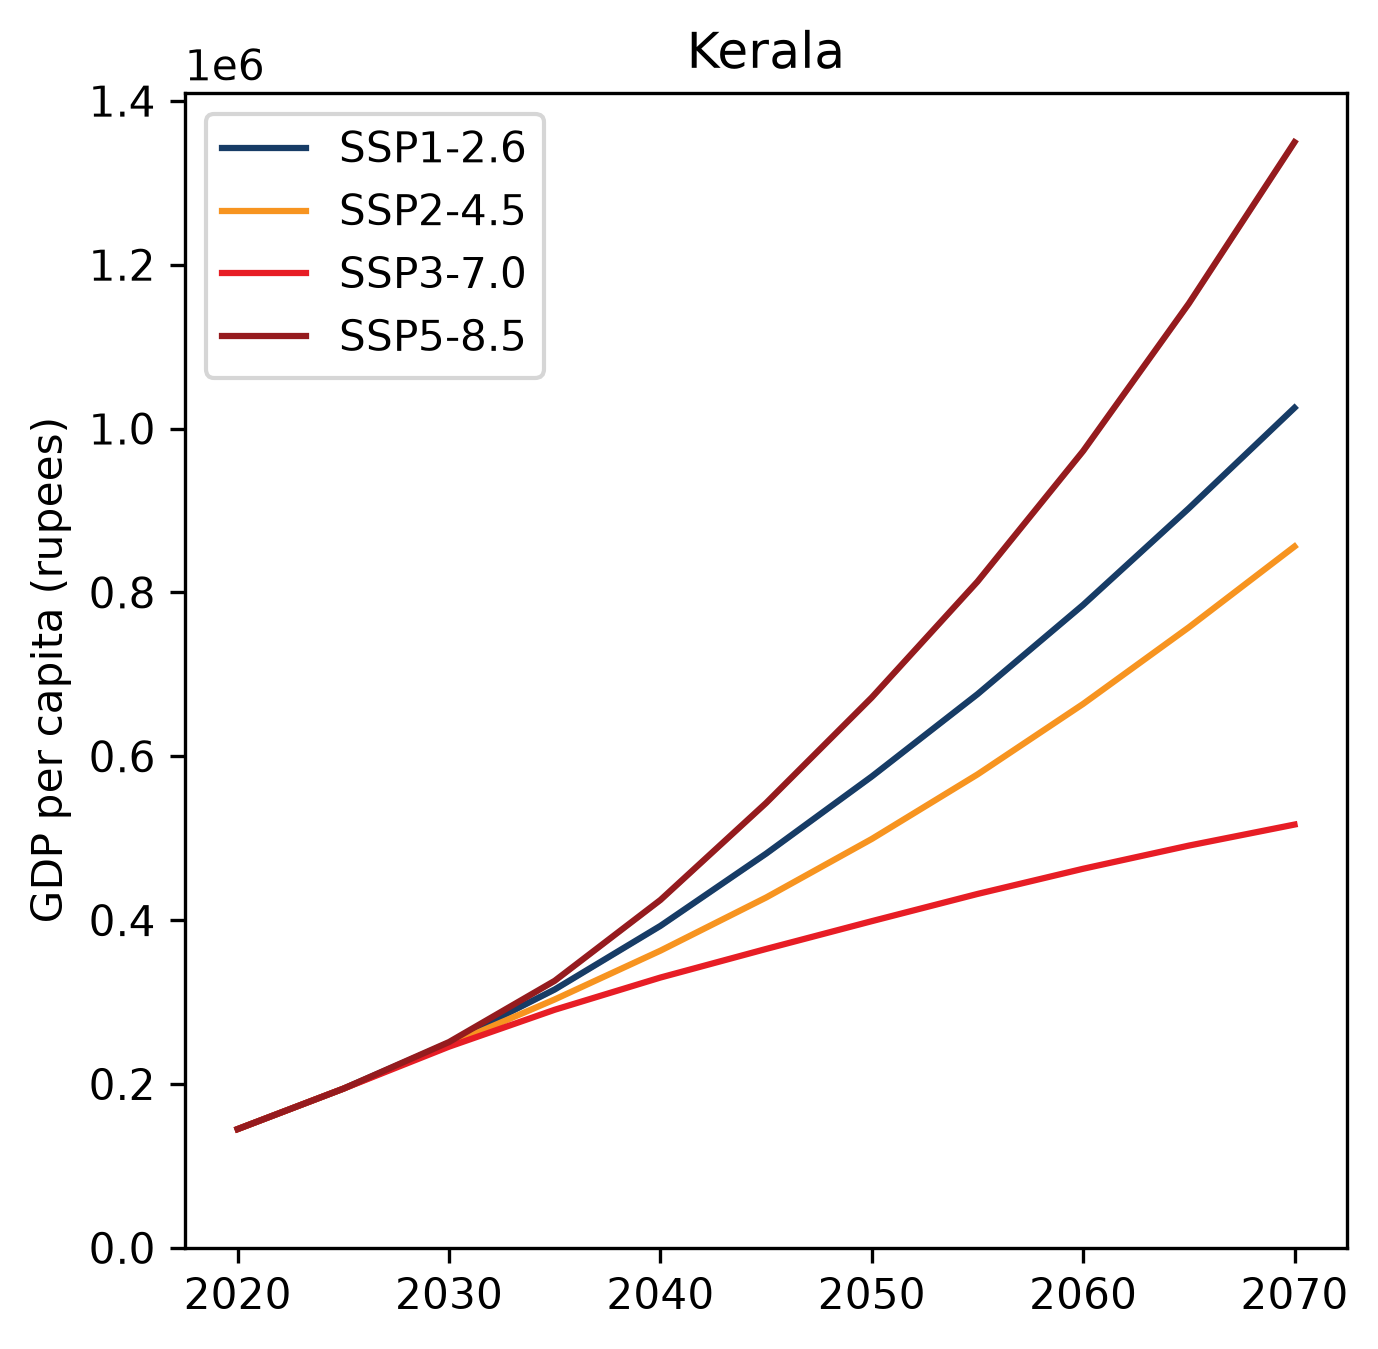
\includegraphics[height=0.25\textheight]{figures/projection_states/projection_gdp_per_capita_Kerala.png}\\
   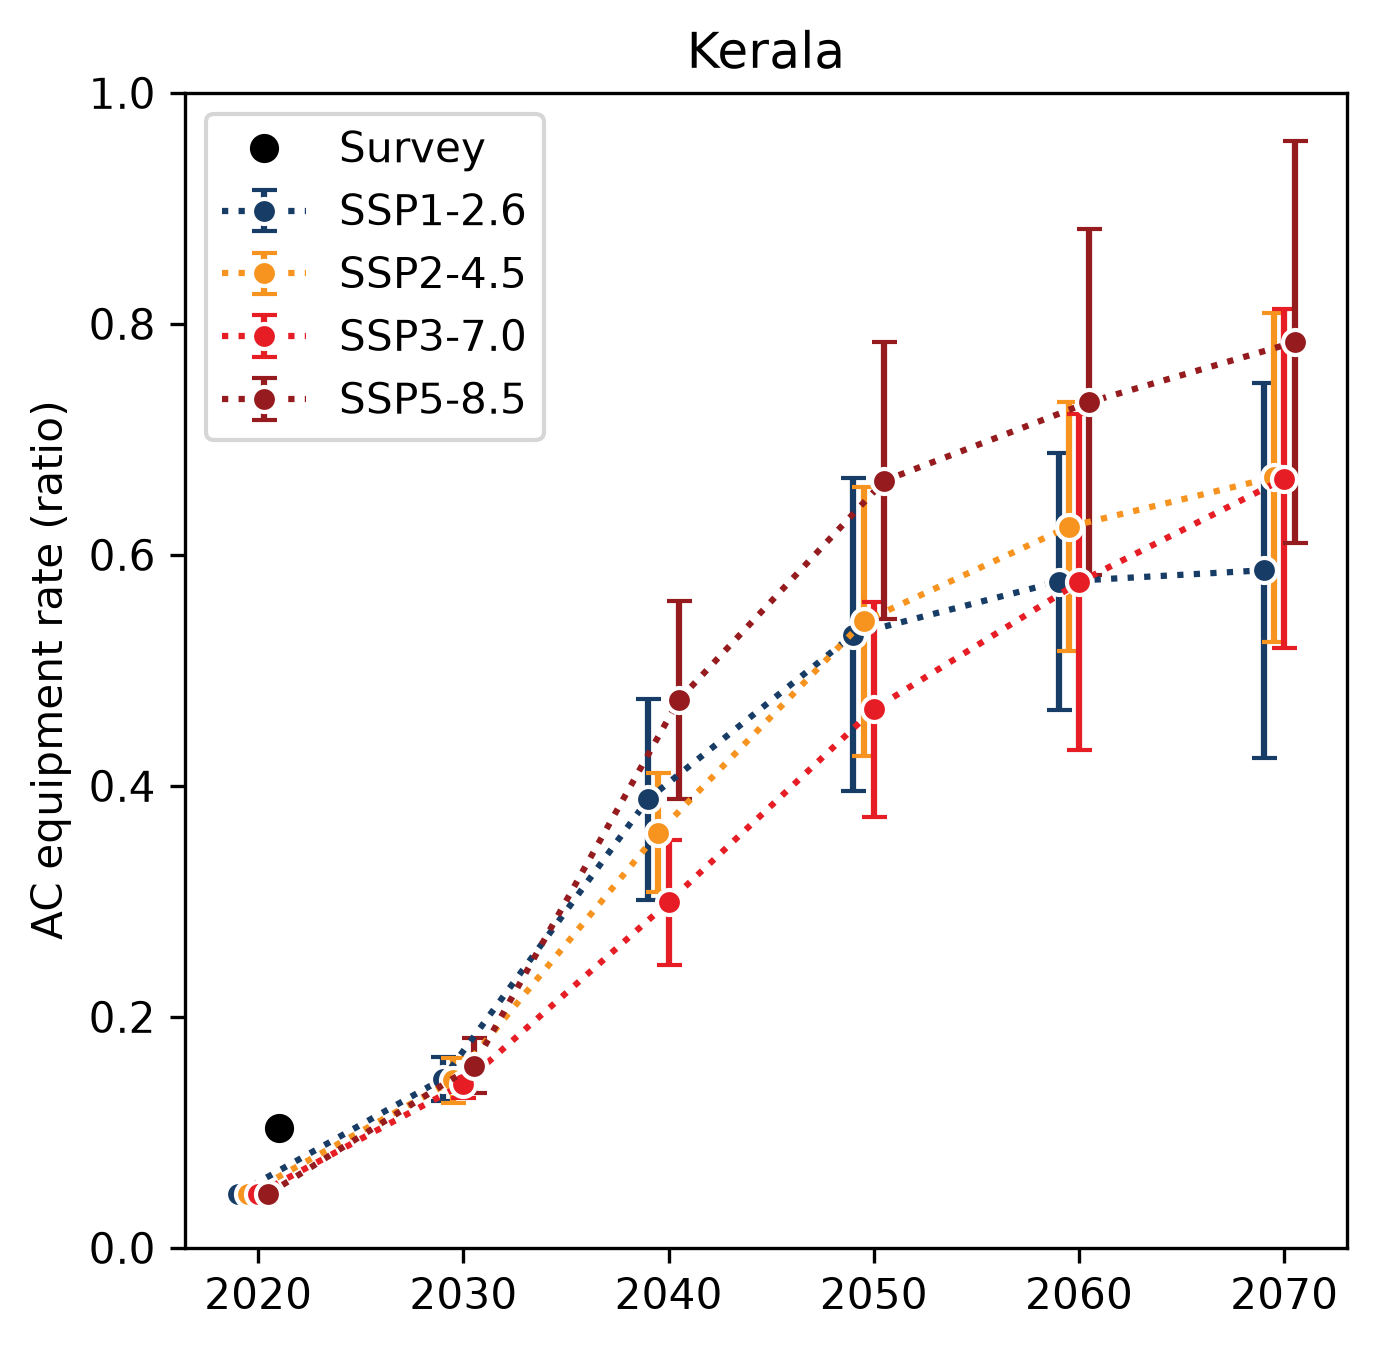
\includegraphics[height=0.25\textheight]{figures/projection_states/projection_ac_rate_Kerala.png}\hfill
   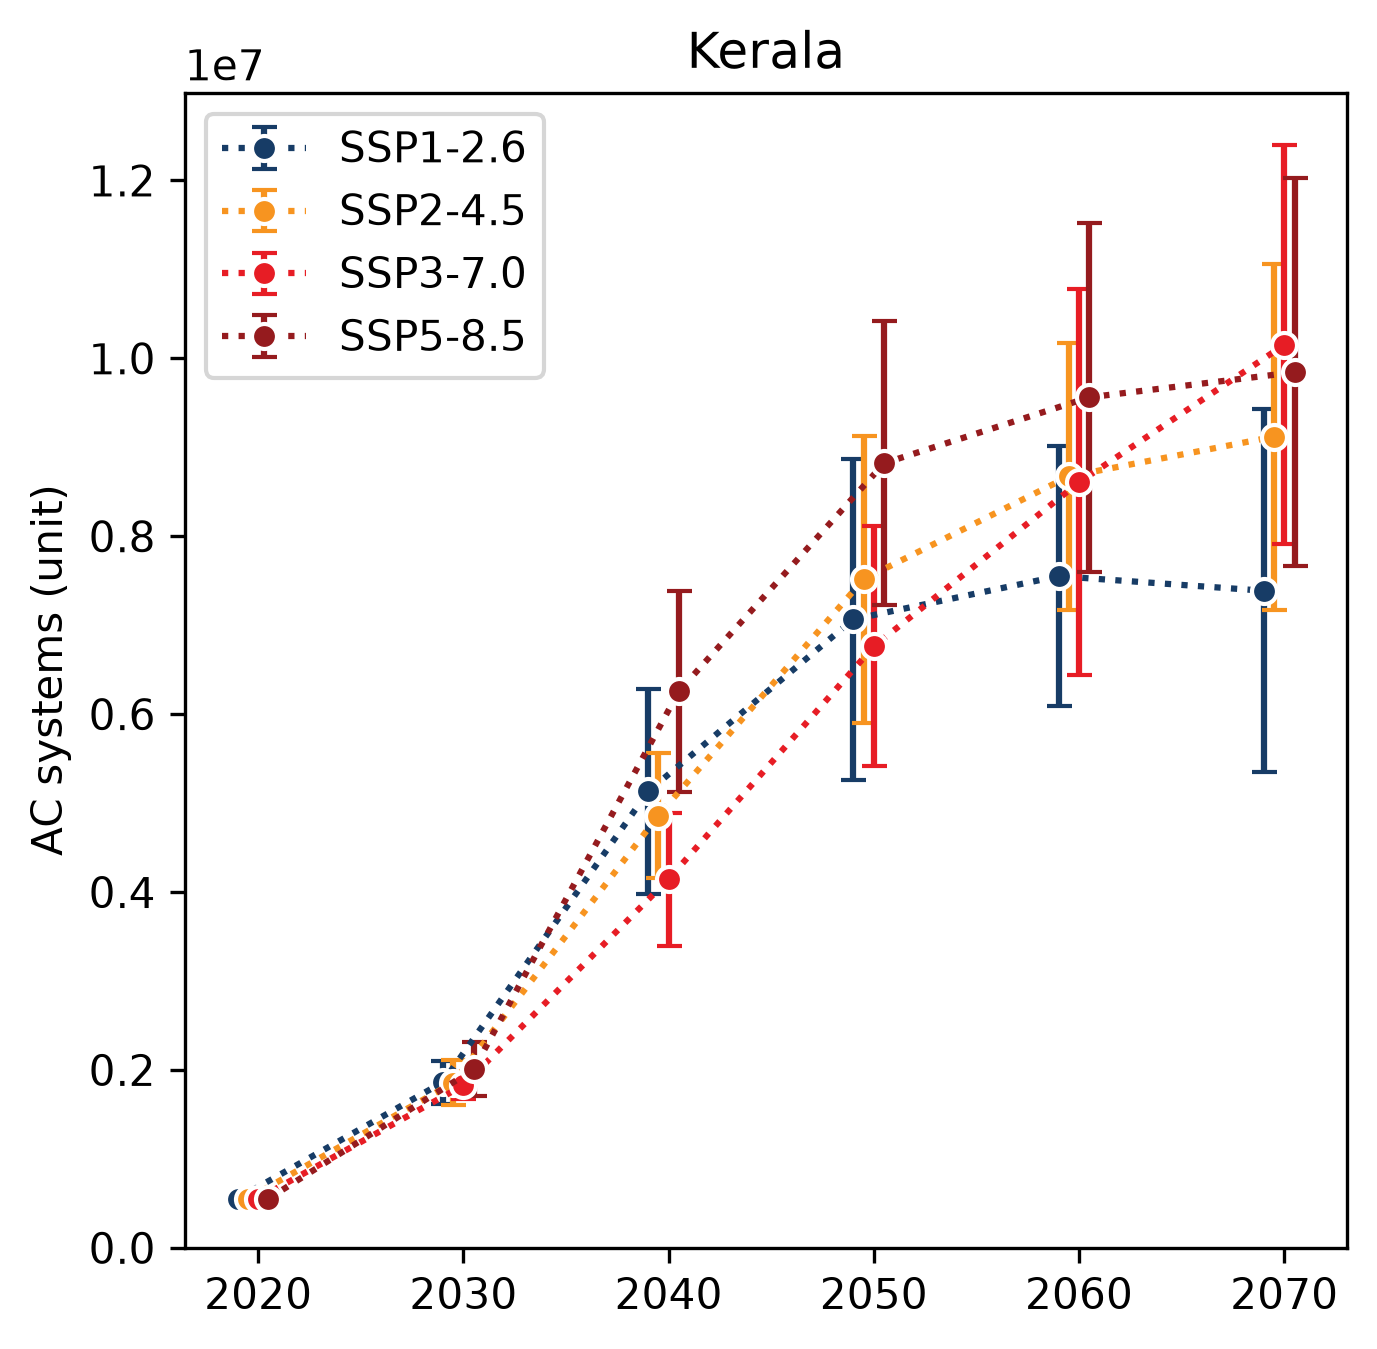
\includegraphics[height=0.25\textheight]{figures/projection_states/projection_ac_systems_Kerala.png}
   \caption{Projections des différentes variables pour Kerala}
\end{figure}

\clearpage

\subsubsection{Madhya Pradesh}

\begin{figure}[ht]
   \centering
   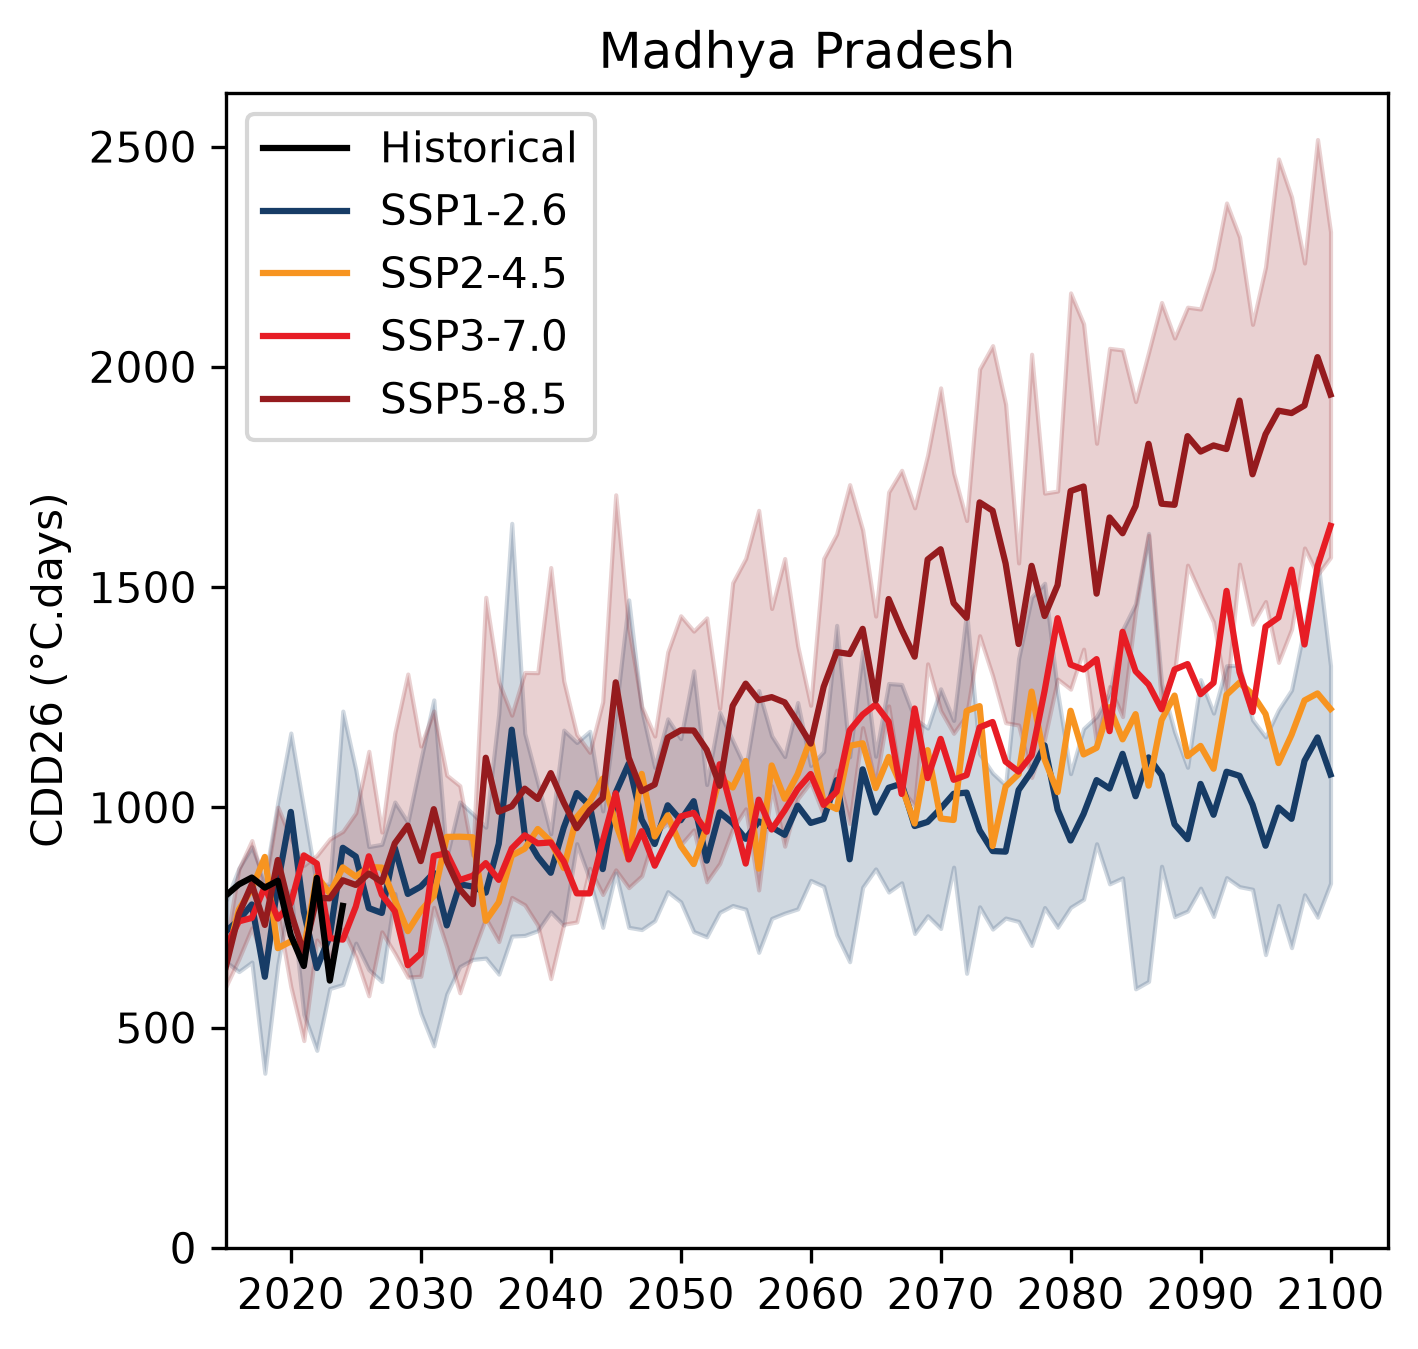
\includegraphics[height=0.25\textheight]{figures/projection_states/projection_cdd26_Madhya Pradesh.png}\hfill
   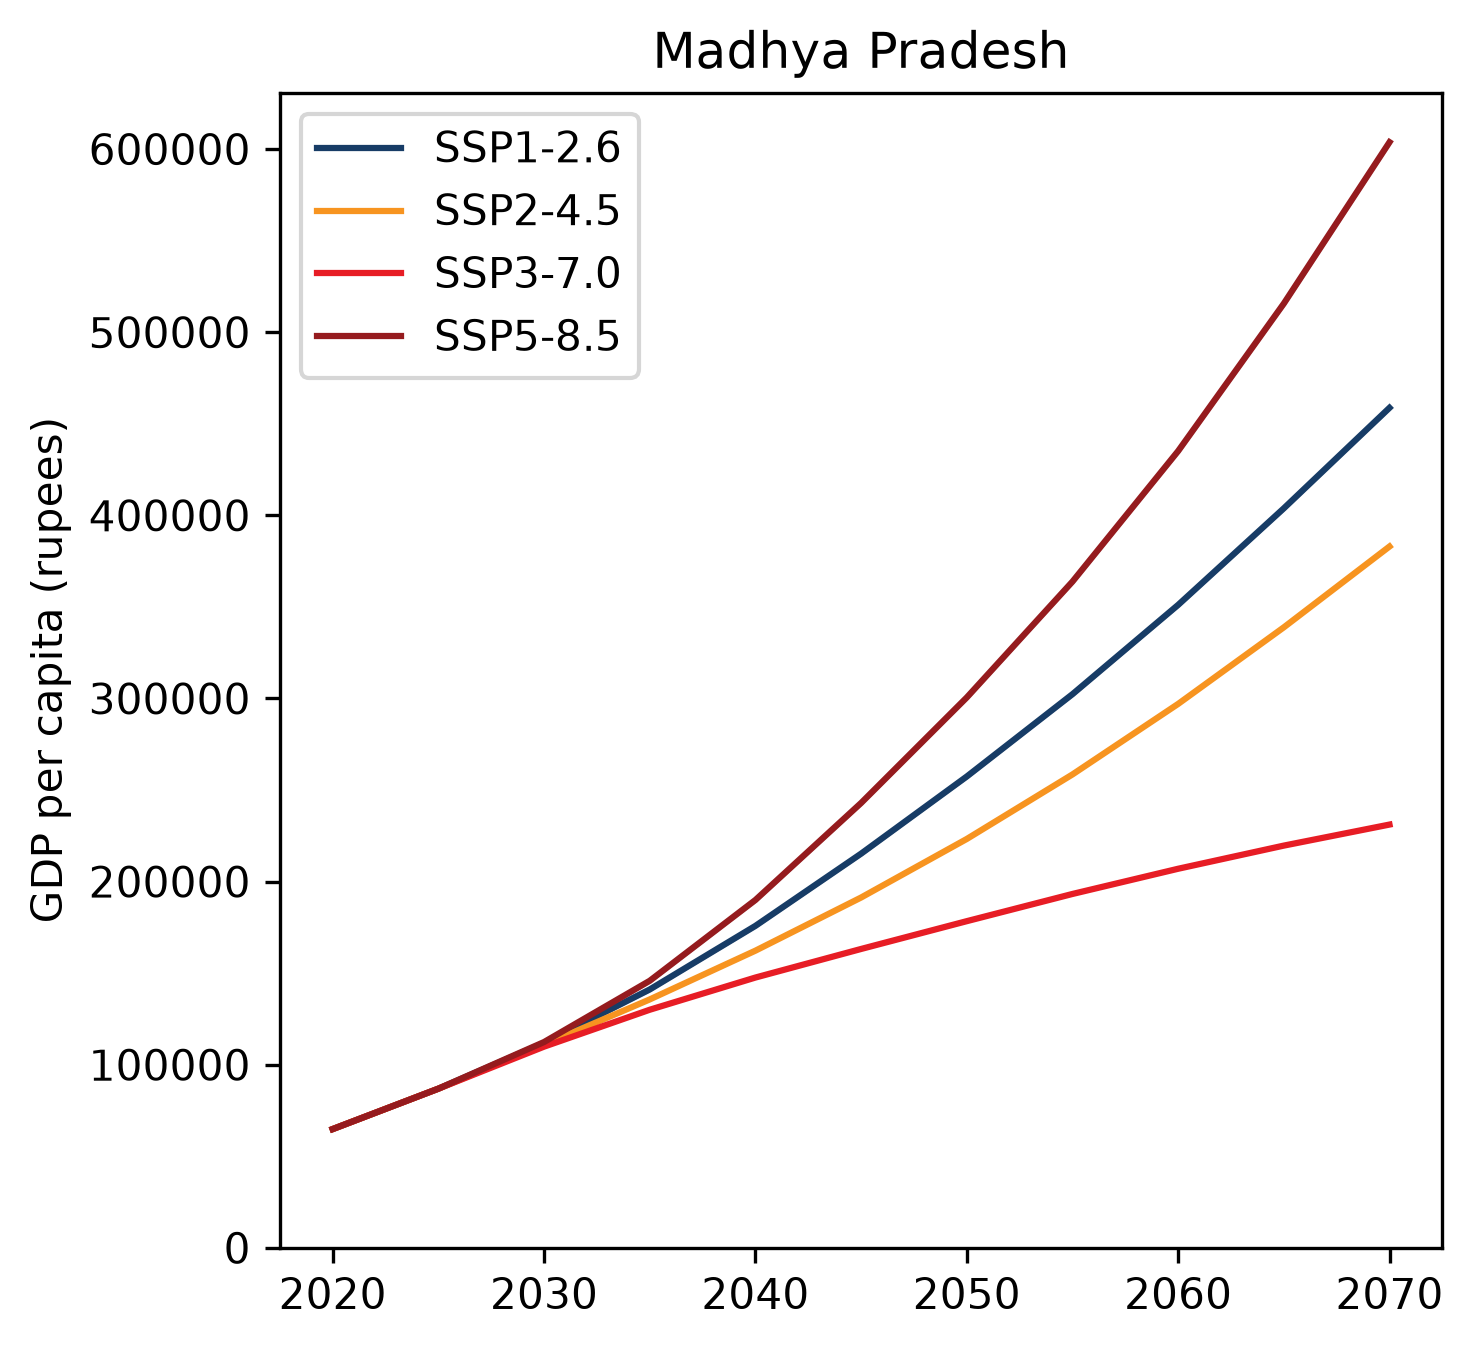
\includegraphics[height=0.25\textheight]{figures/projection_states/projection_gdp_per_capita_Madhya Pradesh.png}\\
   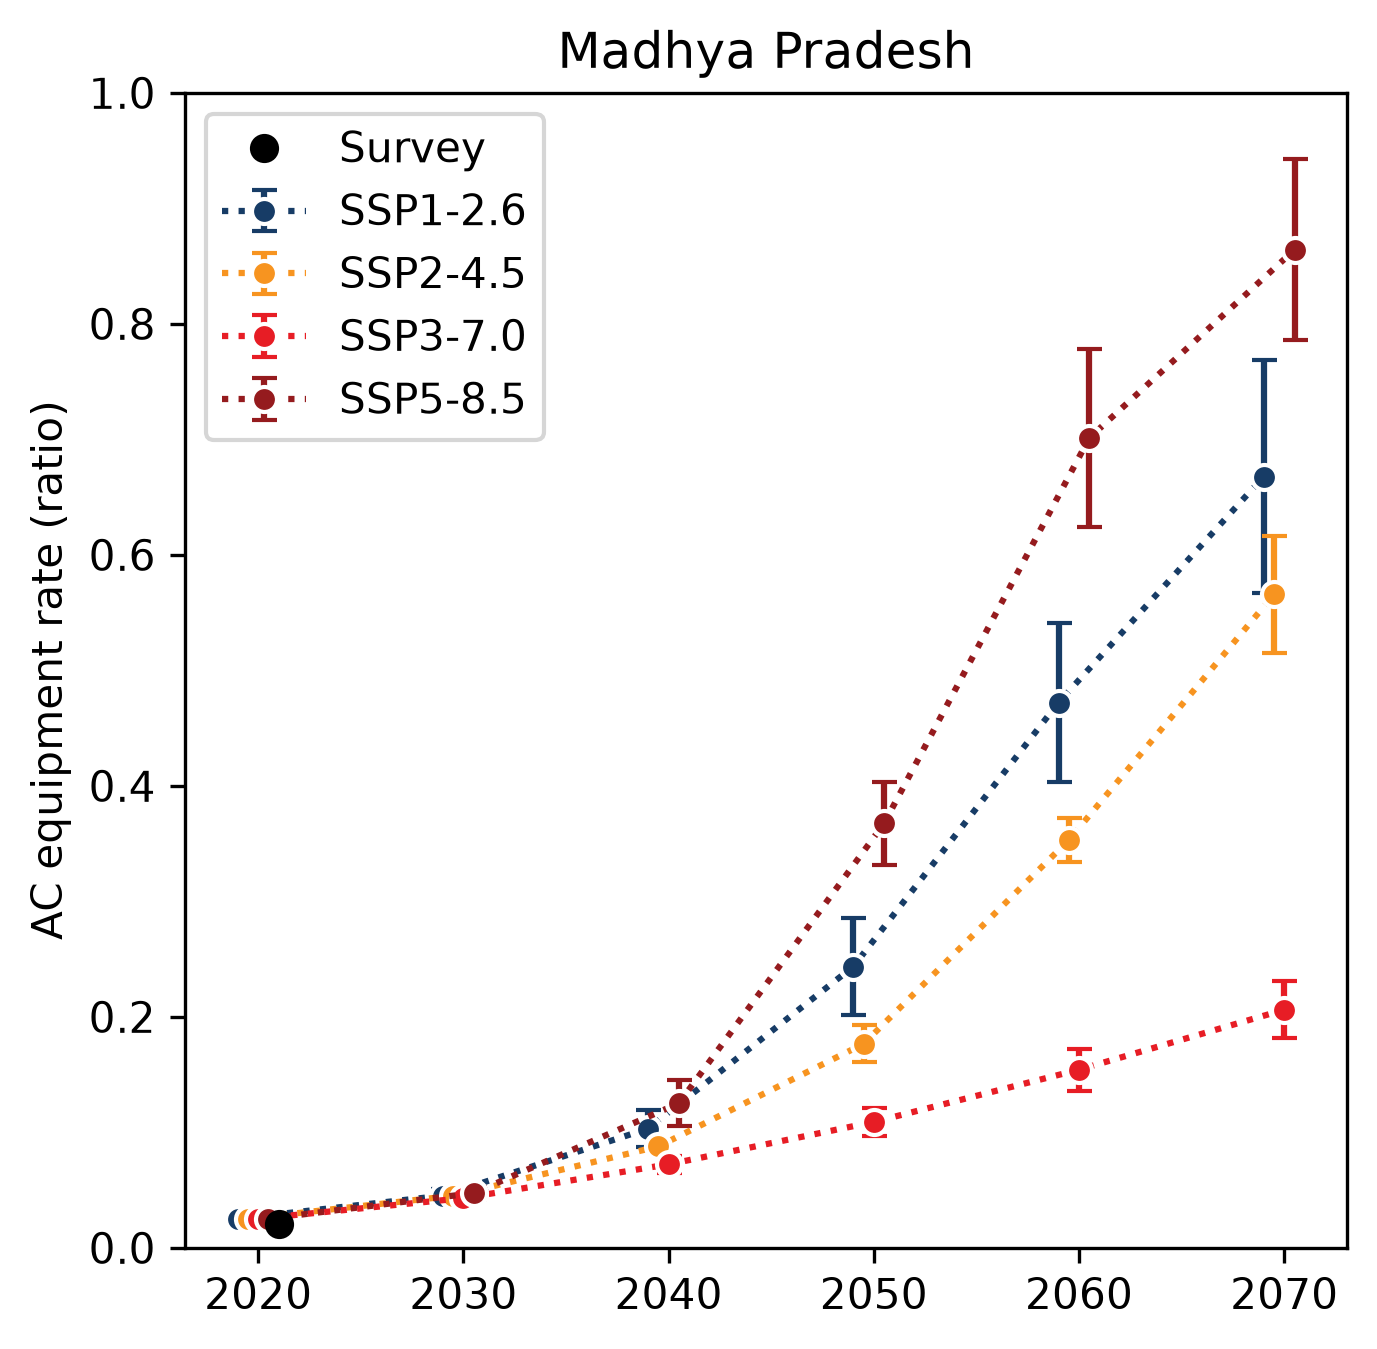
\includegraphics[height=0.25\textheight]{figures/projection_states/projection_ac_rate_Madhya Pradesh.png}\hfill
   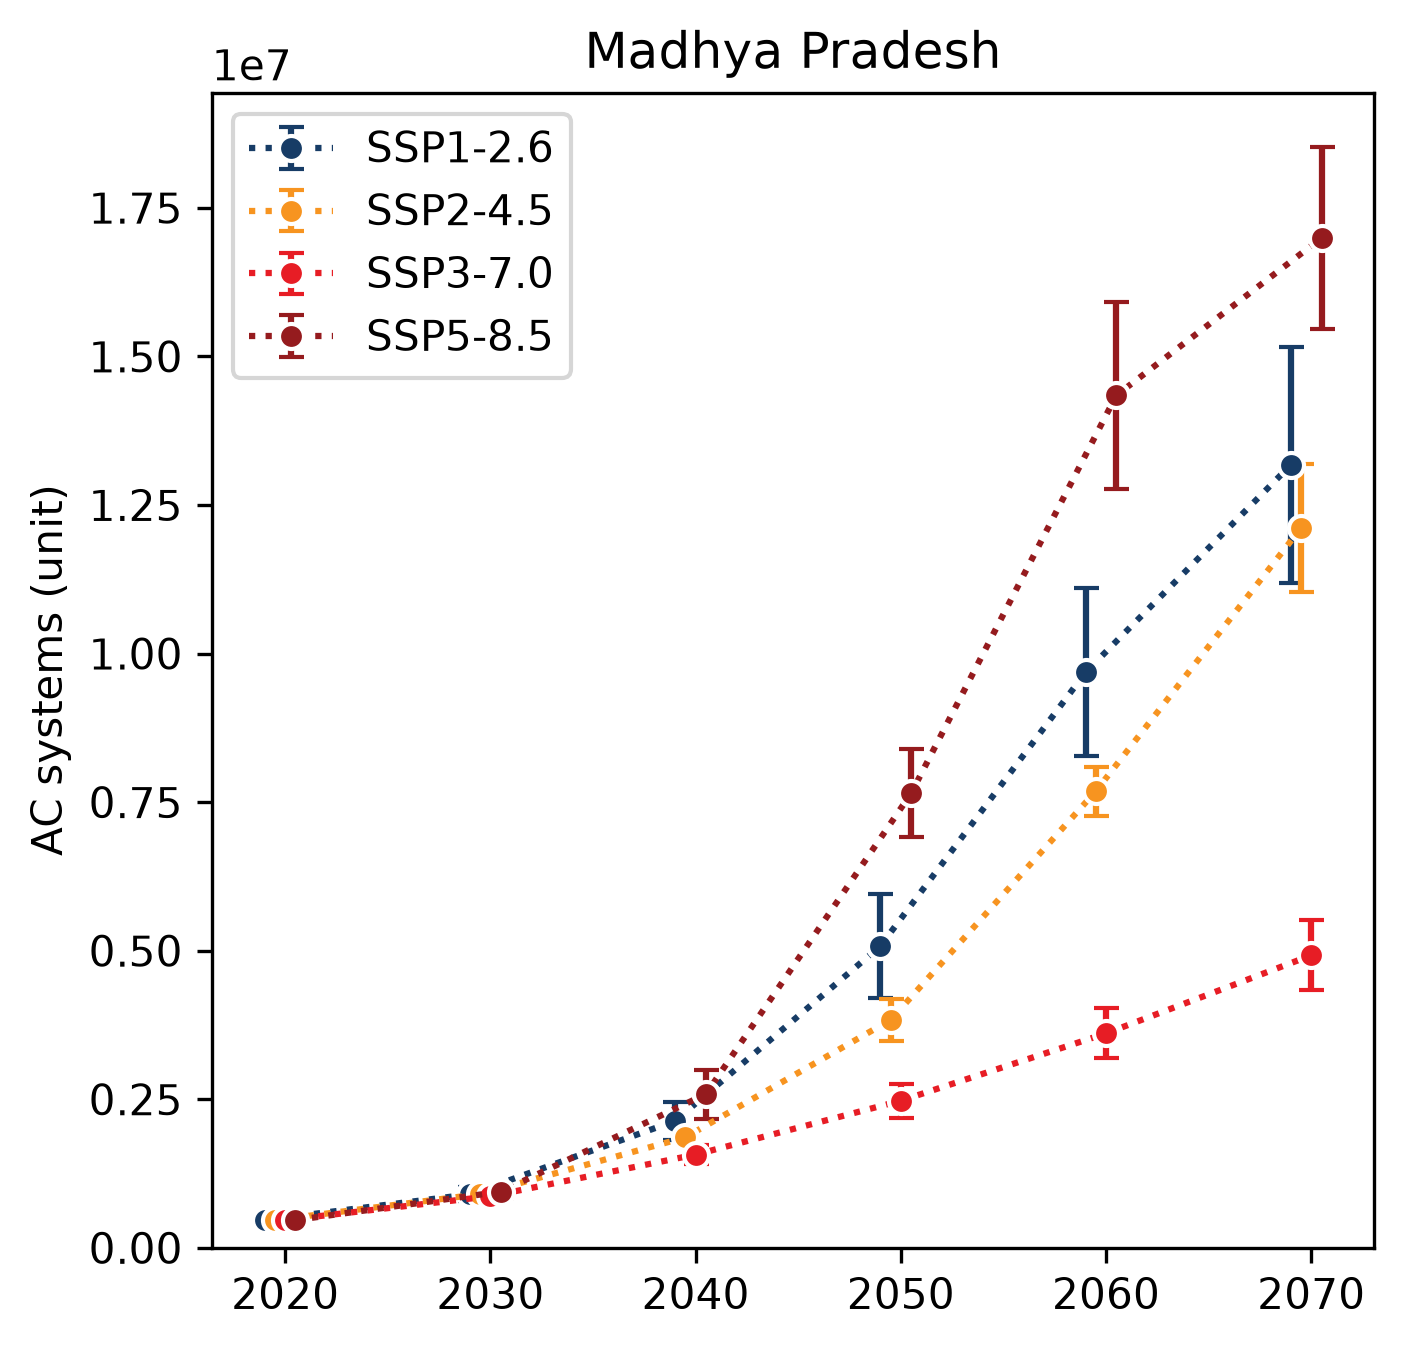
\includegraphics[height=0.25\textheight]{figures/projection_states/projection_ac_systems_Madhya Pradesh.png}
   \caption{Projections des différentes variables pour Madhya Pradesh}
\end{figure}

\clearpage

\subsubsection{Maharashtra}

\begin{figure}[ht]
   \centering
   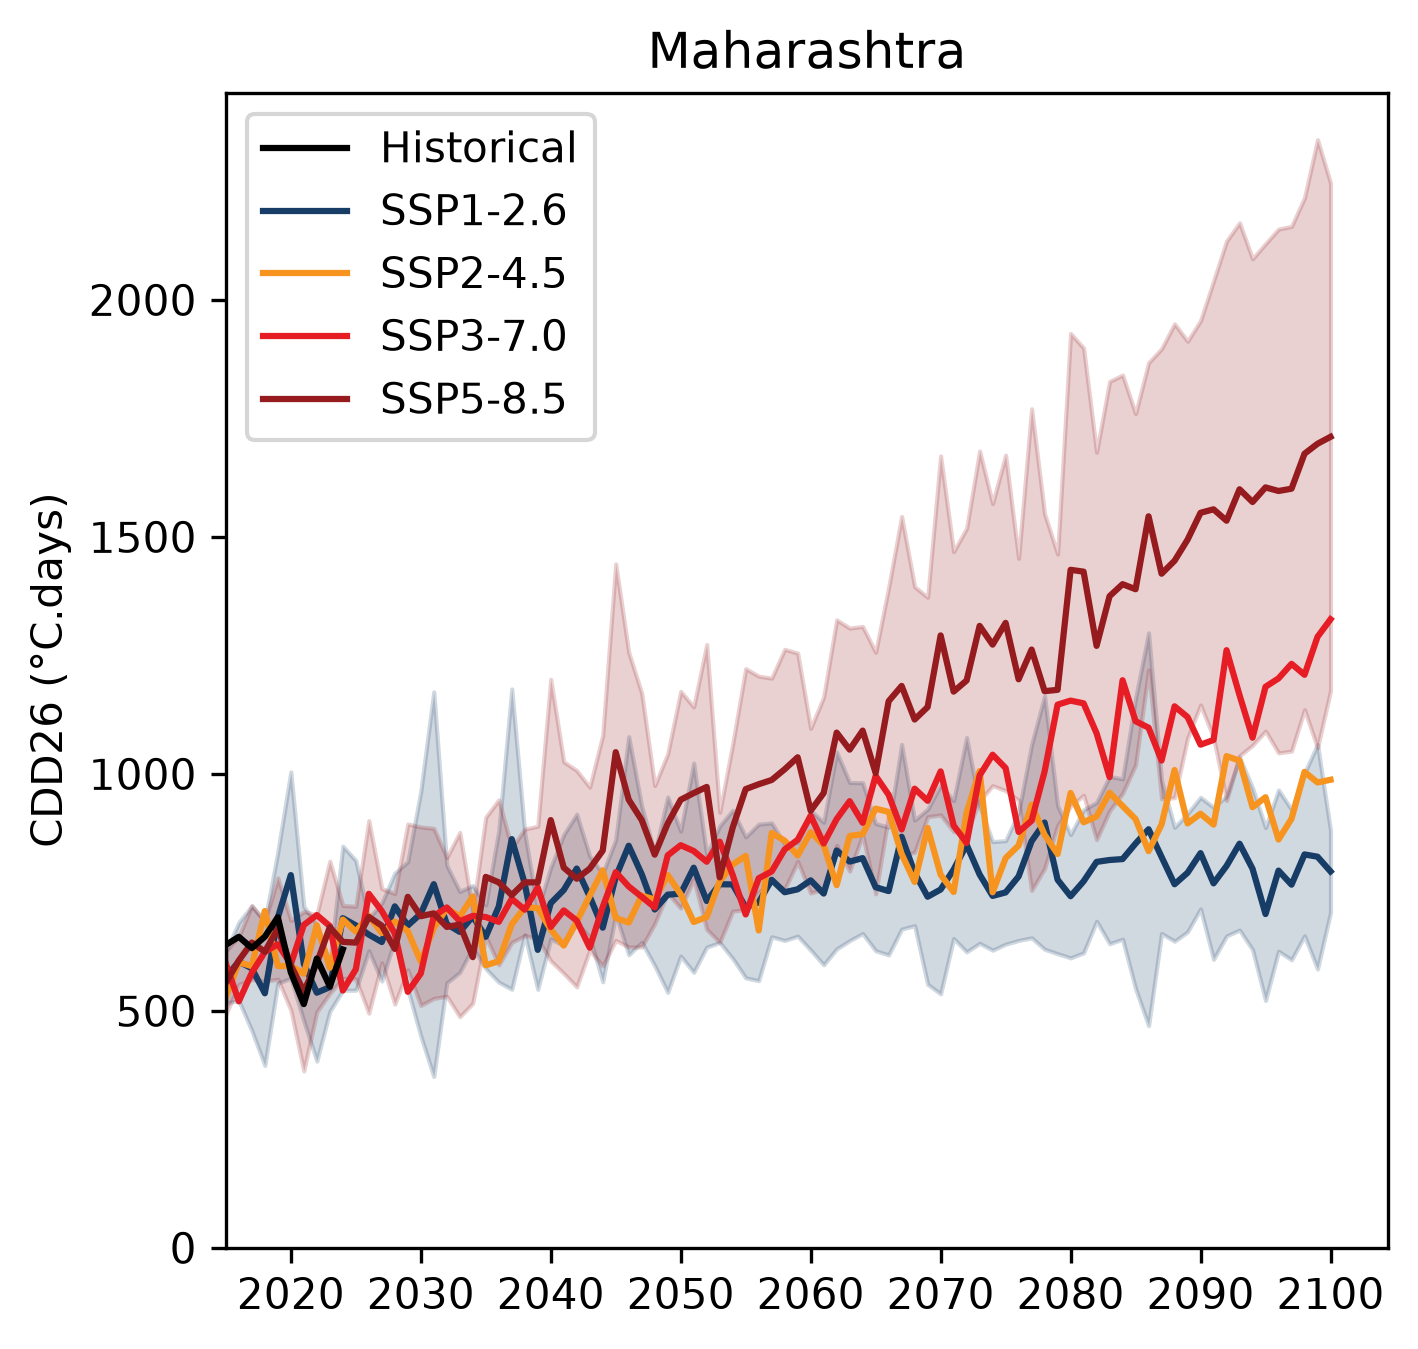
\includegraphics[height=0.25\textheight]{figures/projection_states/projection_cdd26_Maharashtra.png}\hfill
   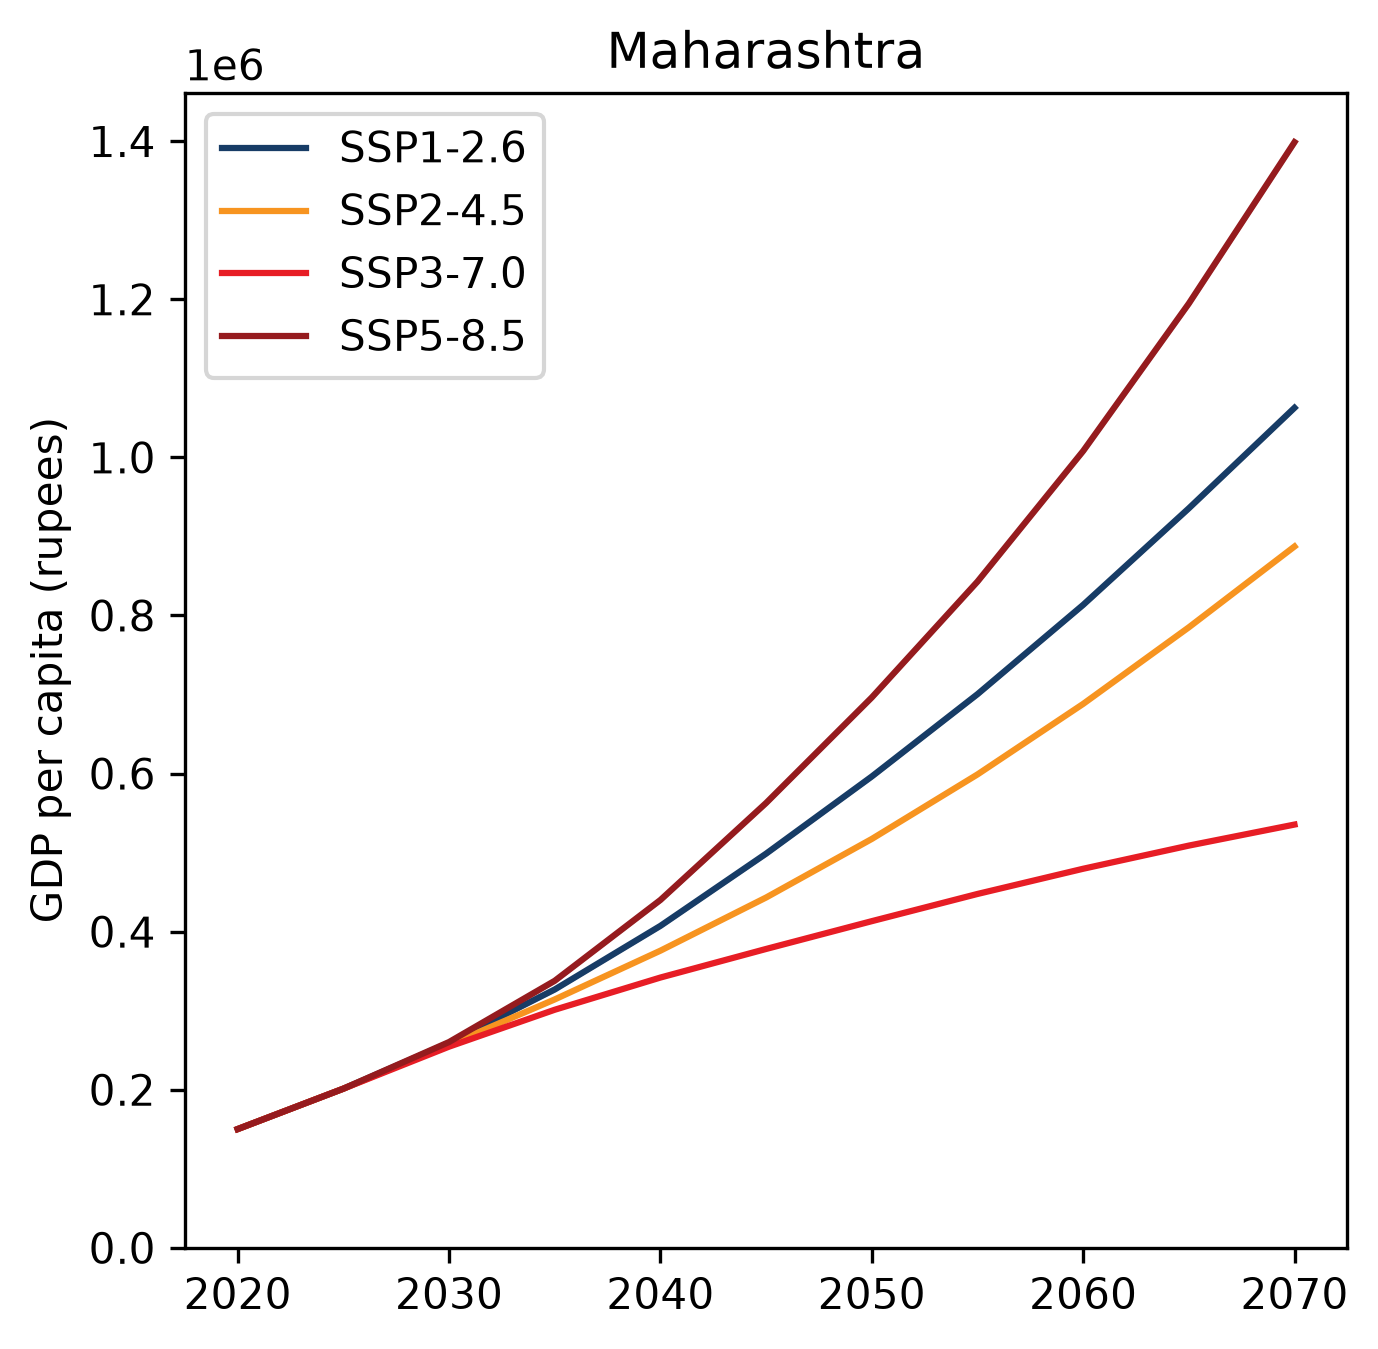
\includegraphics[height=0.25\textheight]{figures/projection_states/projection_gdp_per_capita_Maharashtra.png}\\
   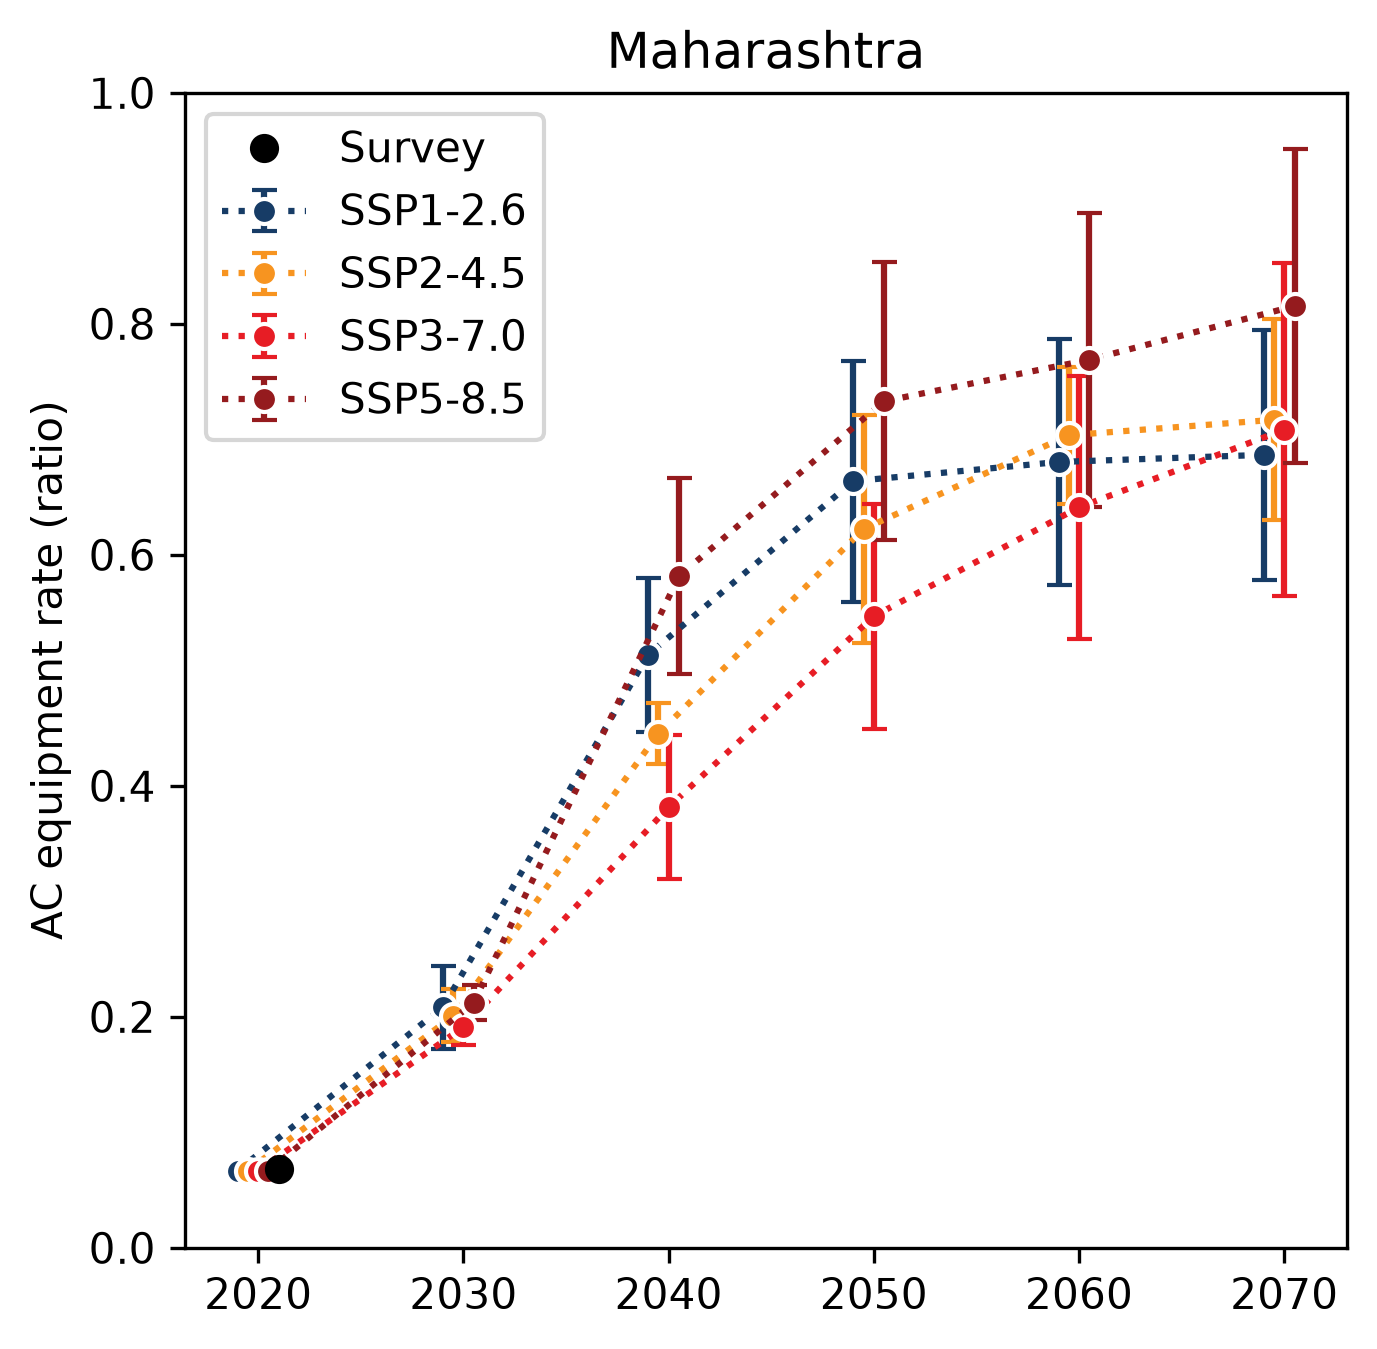
\includegraphics[height=0.25\textheight]{figures/projection_states/projection_ac_rate_Maharashtra.png}\hfill
   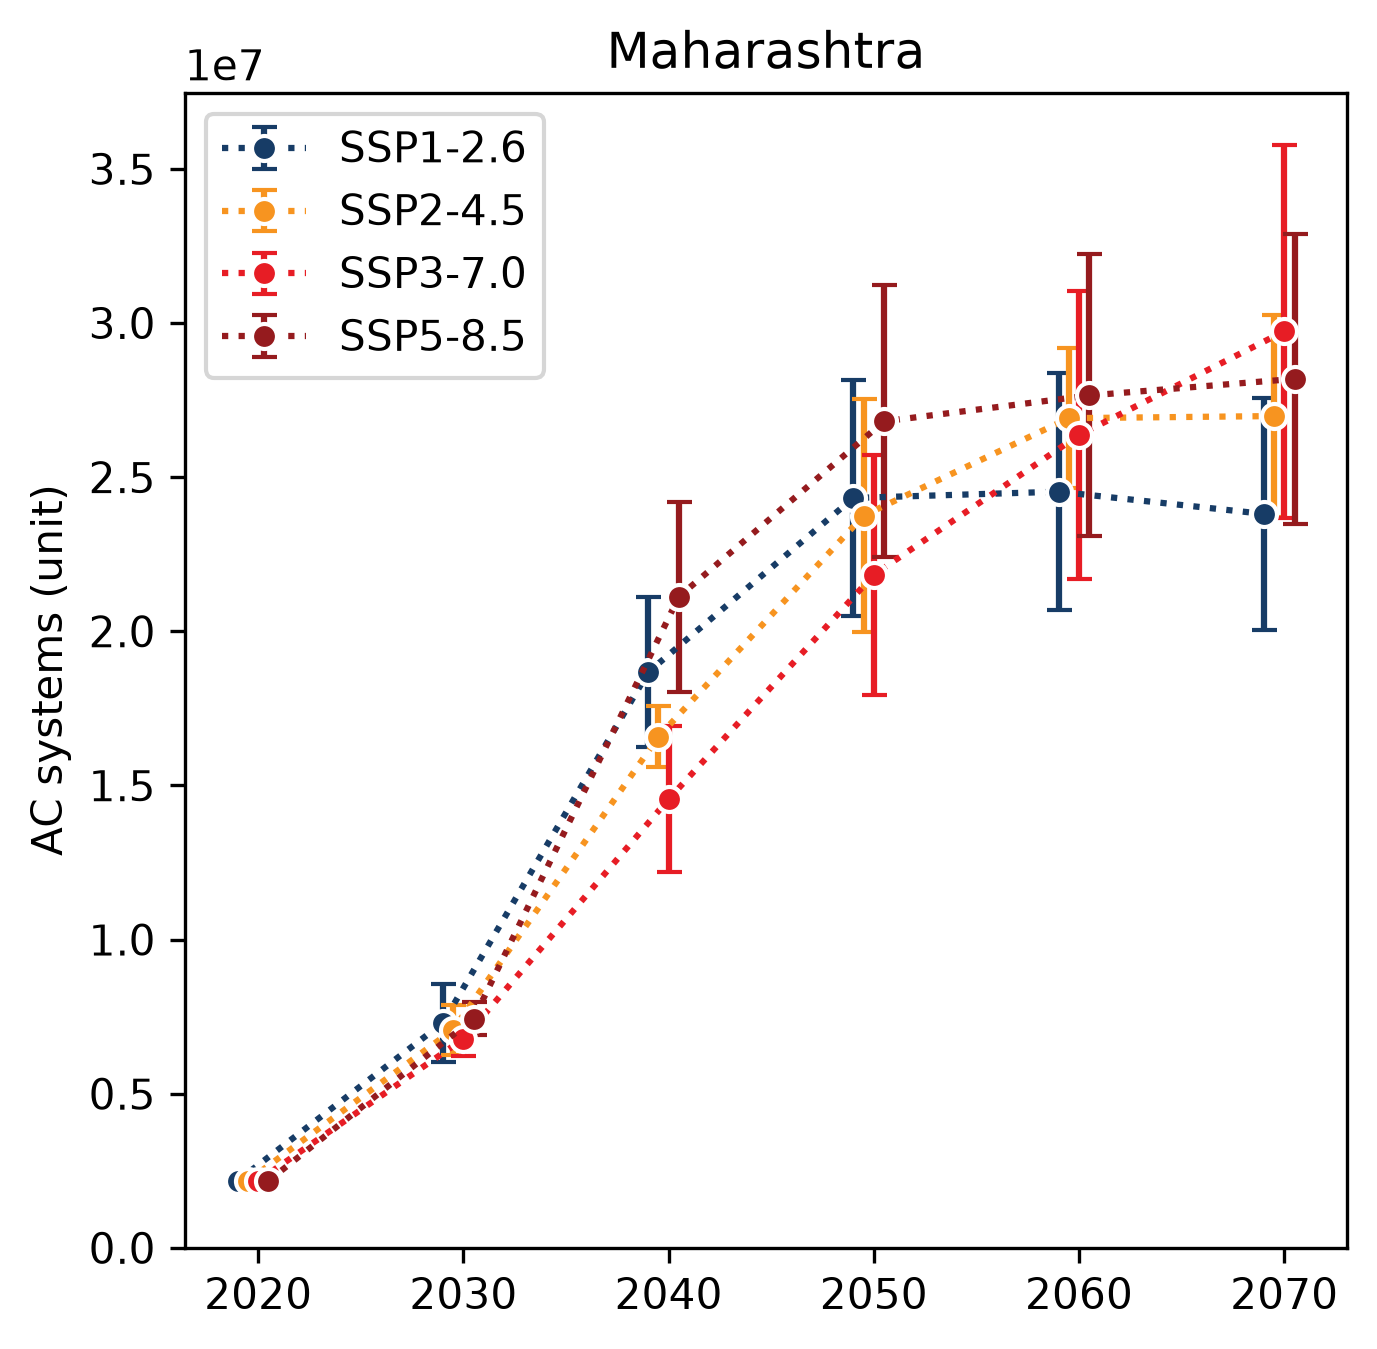
\includegraphics[height=0.25\textheight]{figures/projection_states/projection_ac_systems_Maharashtra.png}
   \caption{Projections des différentes variables pour Maharashtra}
\end{figure}

\clearpage

\subsubsection{Manipur}

\begin{figure}[ht]
   \centering
   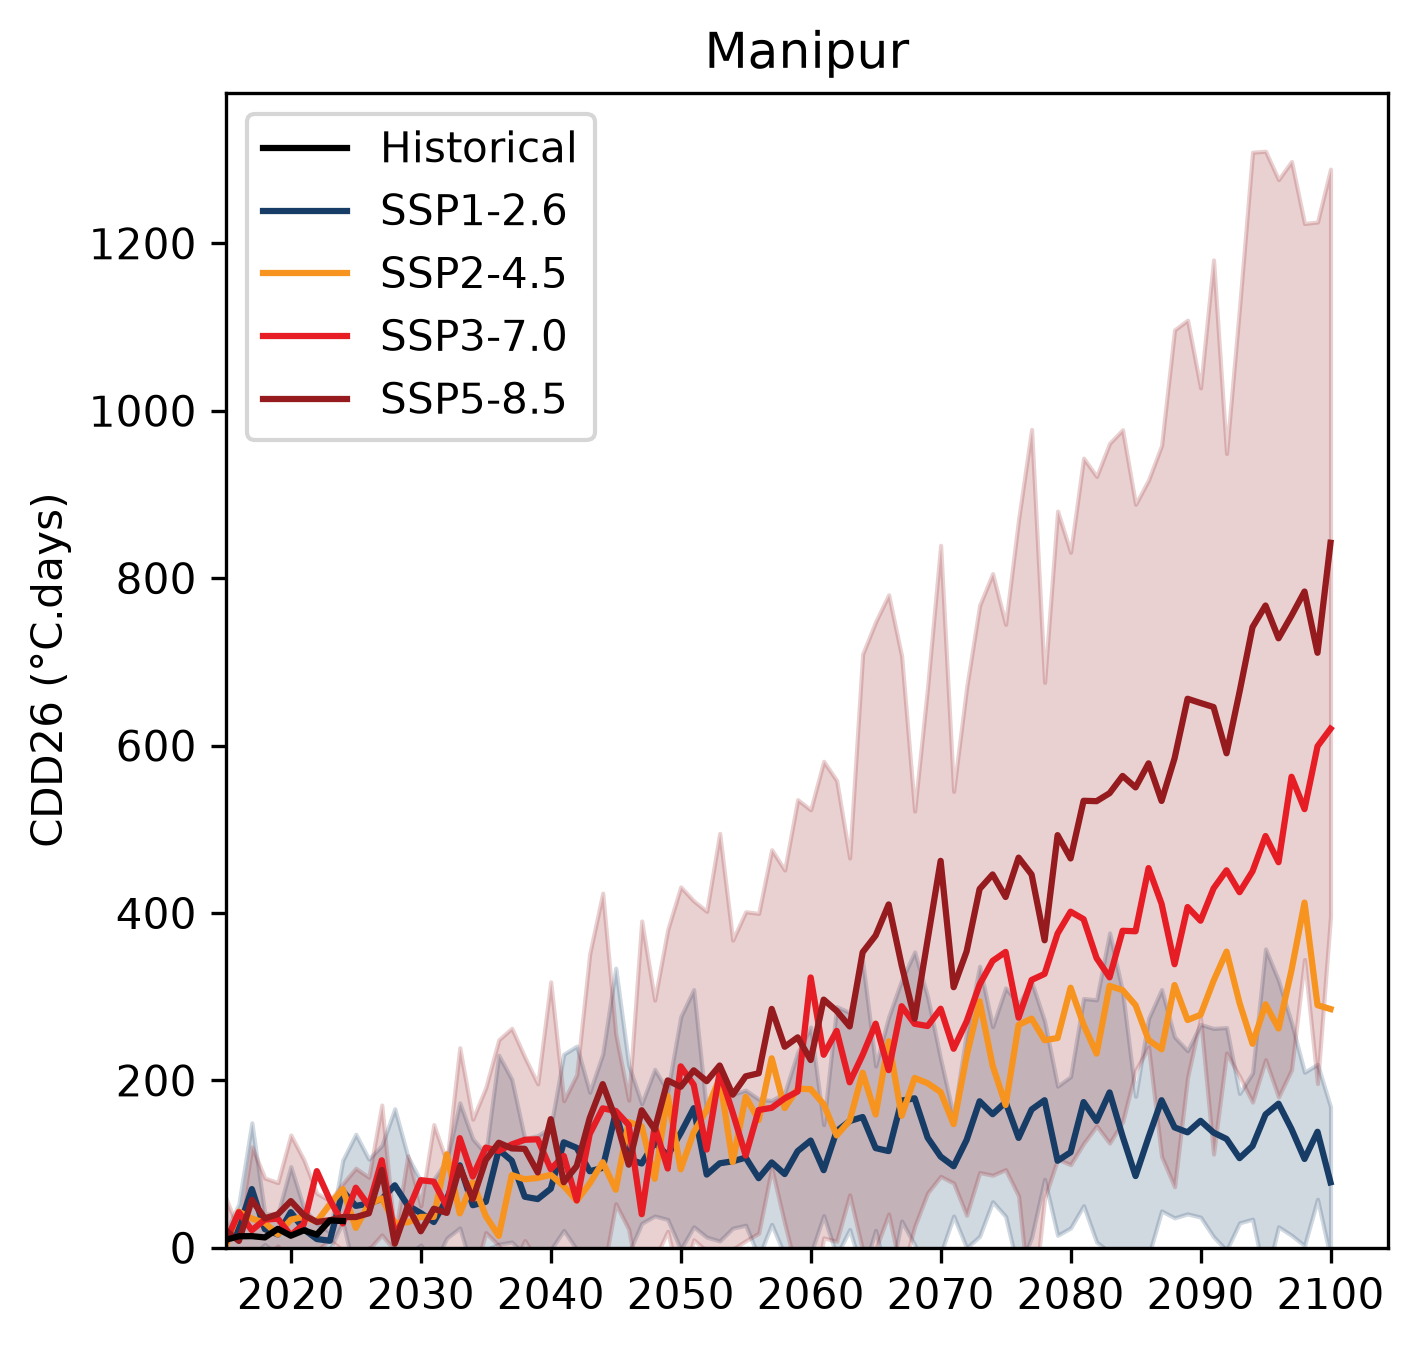
\includegraphics[height=0.25\textheight]{figures/projection_states/projection_cdd26_Manipur.png}\hfill
   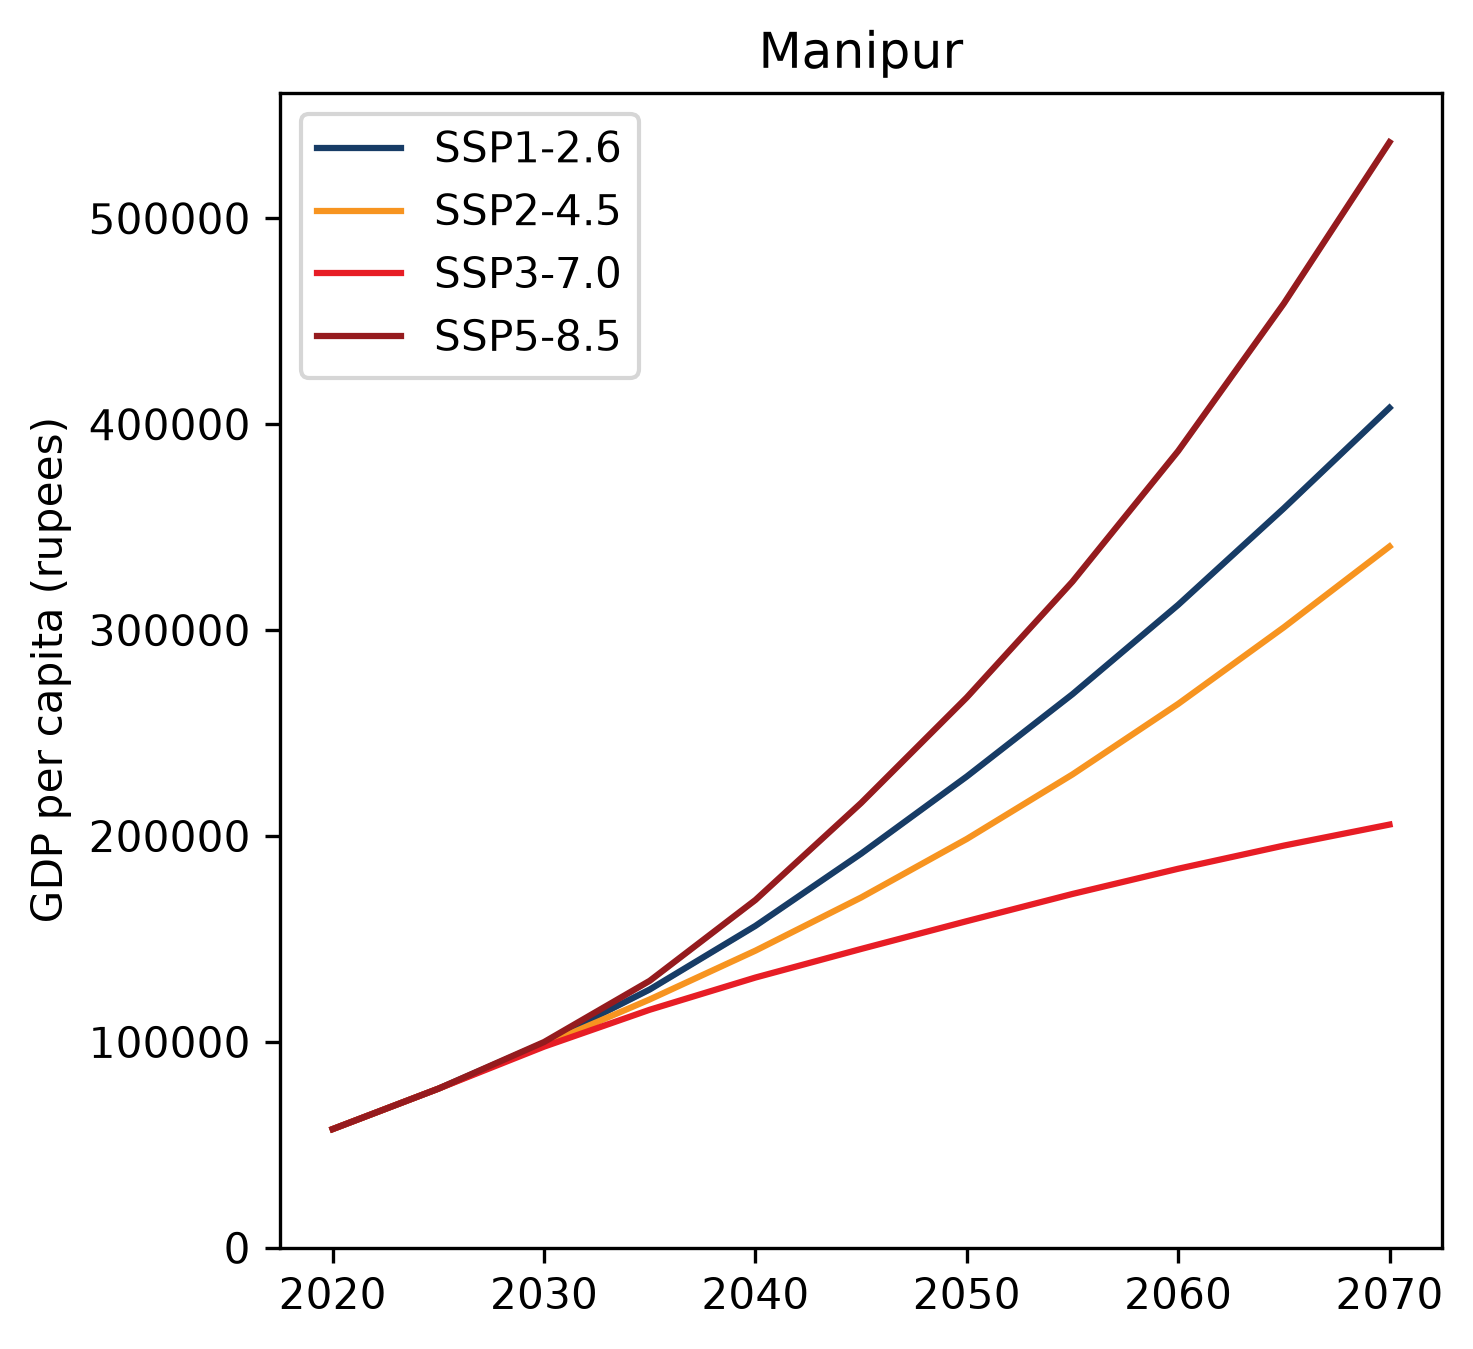
\includegraphics[height=0.25\textheight]{figures/projection_states/projection_gdp_per_capita_Manipur.png}\\
   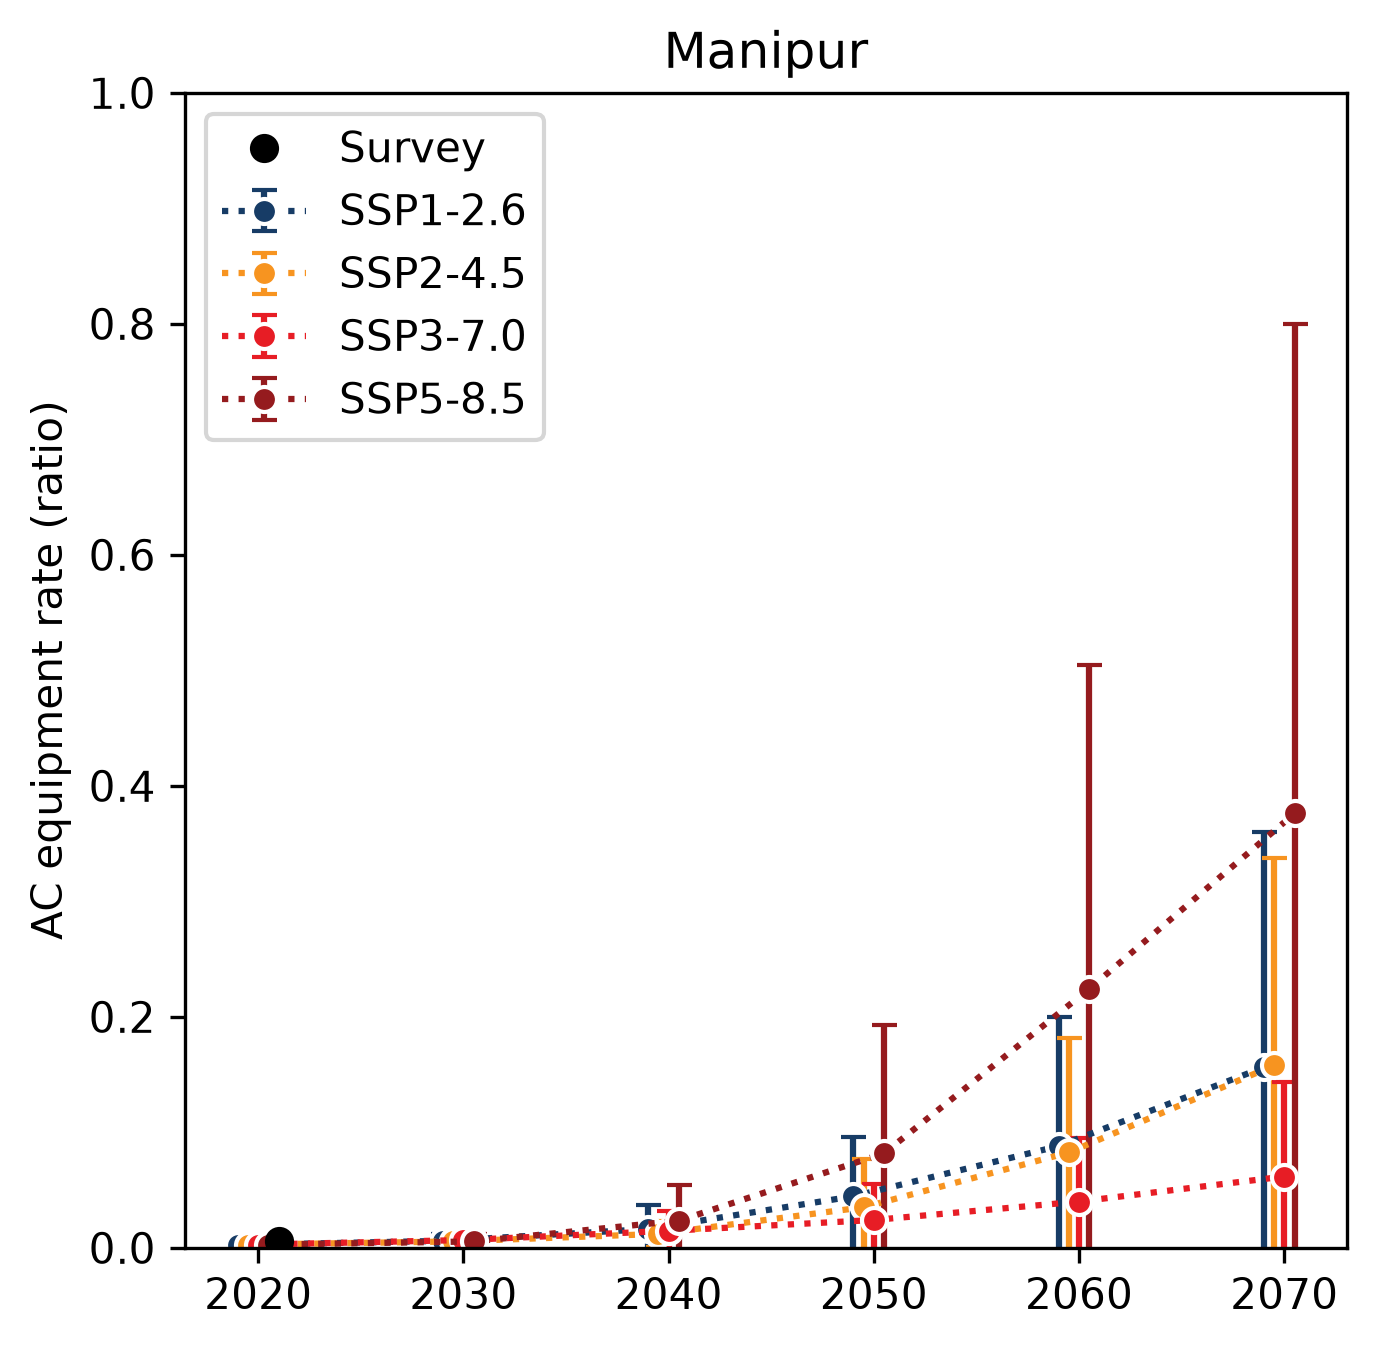
\includegraphics[height=0.25\textheight]{figures/projection_states/projection_ac_rate_Manipur.png}\hfill
   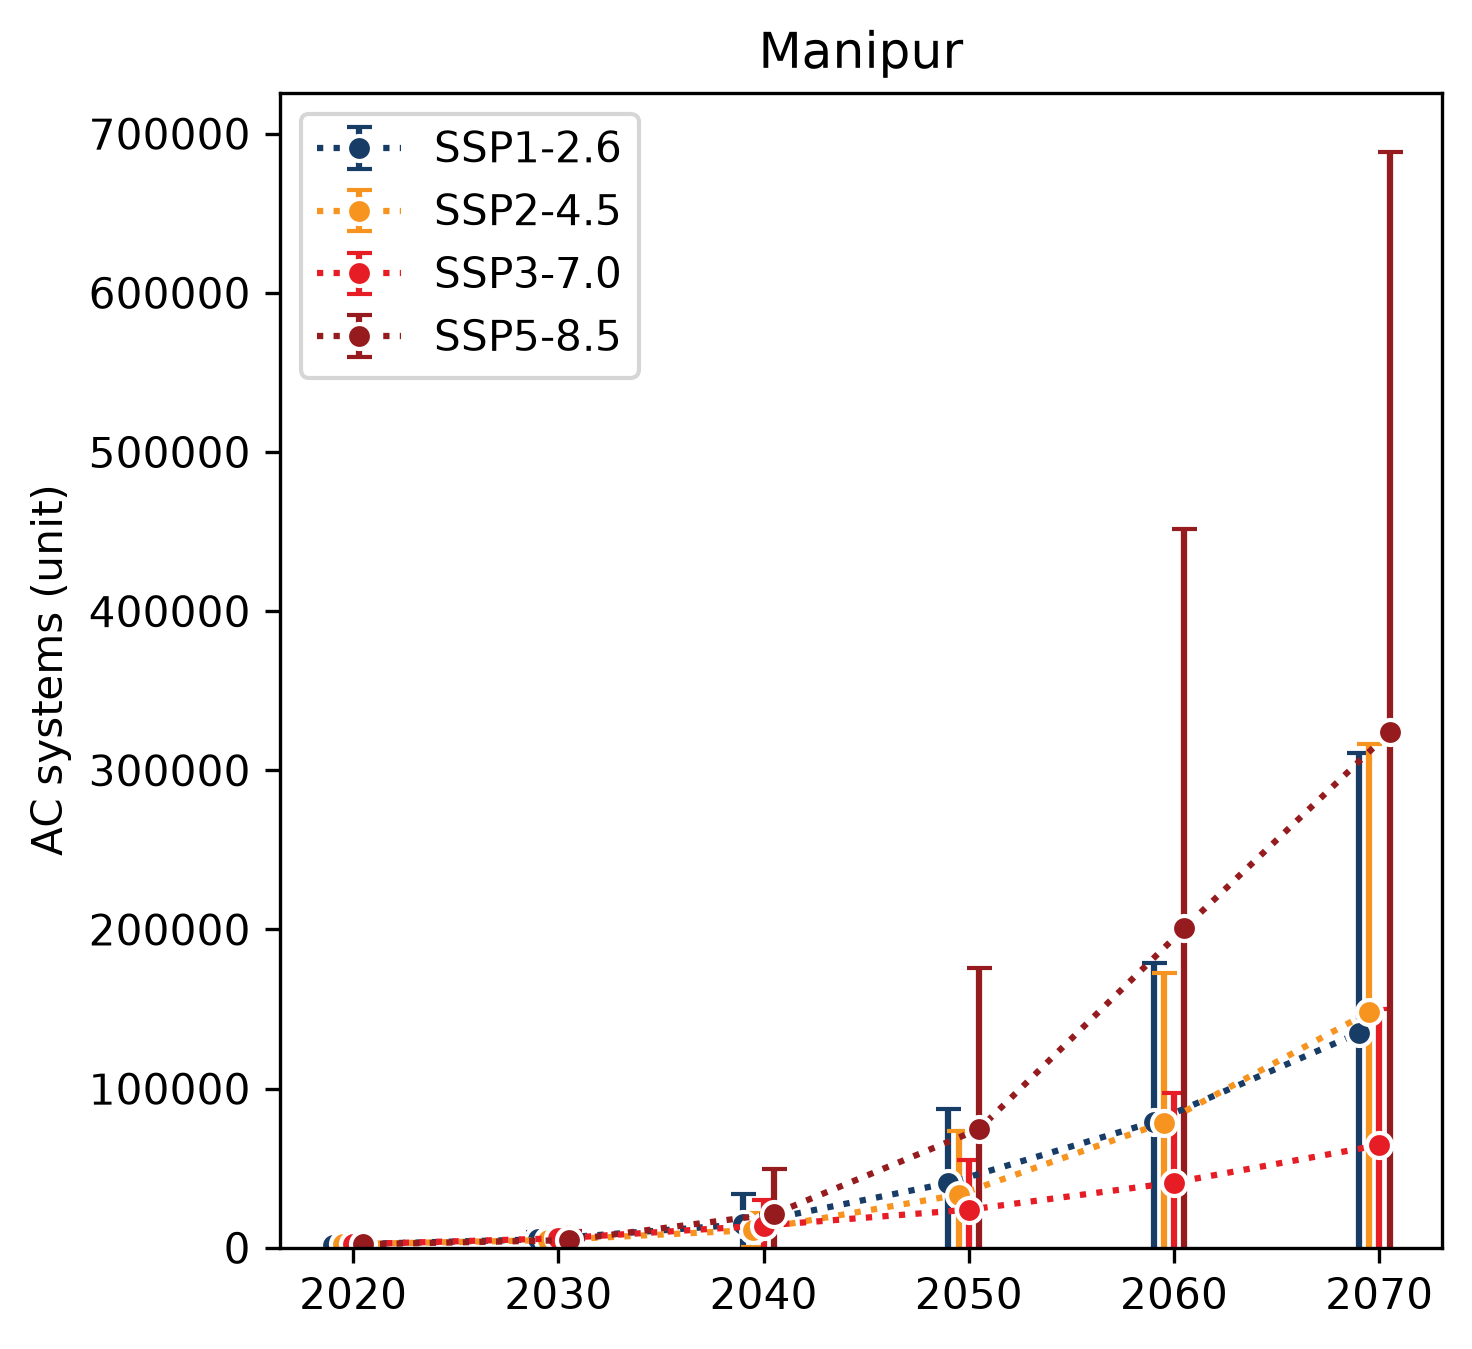
\includegraphics[height=0.25\textheight]{figures/projection_states/projection_ac_systems_Manipur.png}
   \caption{Projections des différentes variables pour Manipur}
\end{figure}

\clearpage

\subsubsection{Meghalaya}

\begin{figure}[ht]
   \centering
   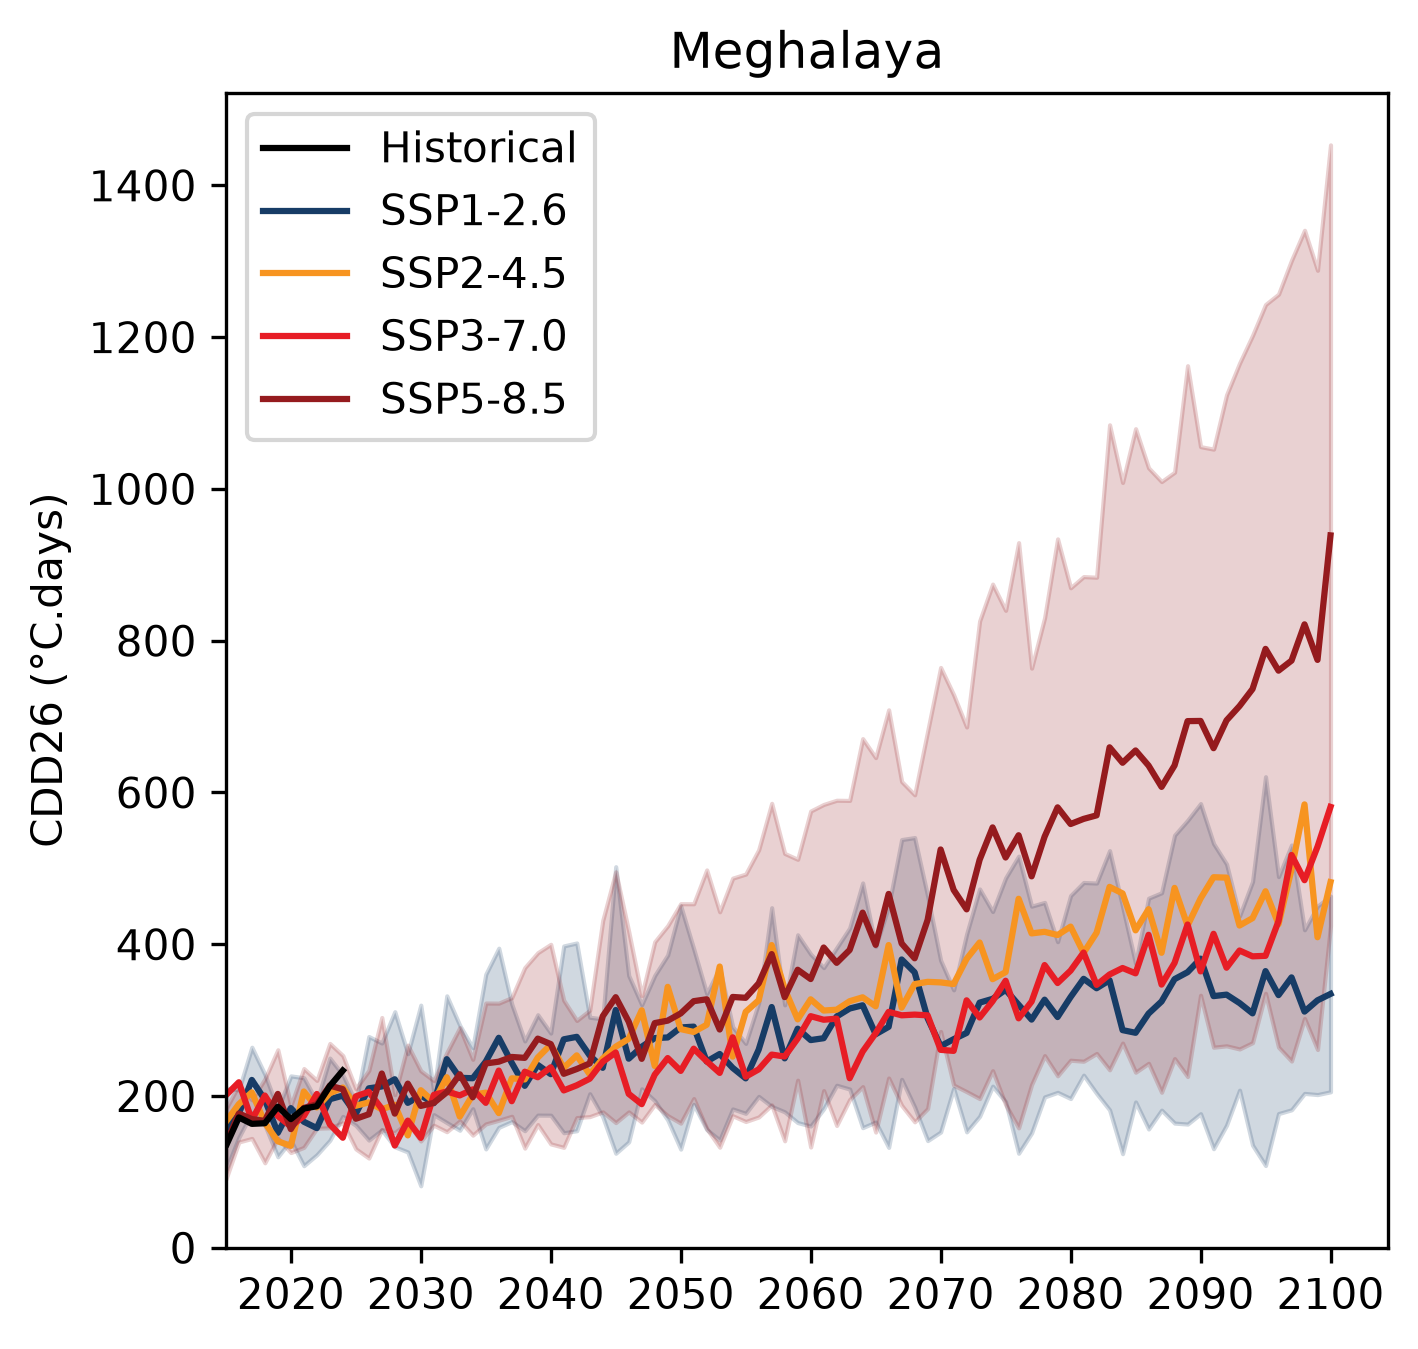
\includegraphics[height=0.25\textheight]{figures/projection_states/projection_cdd26_Meghalaya.png}\hfill
   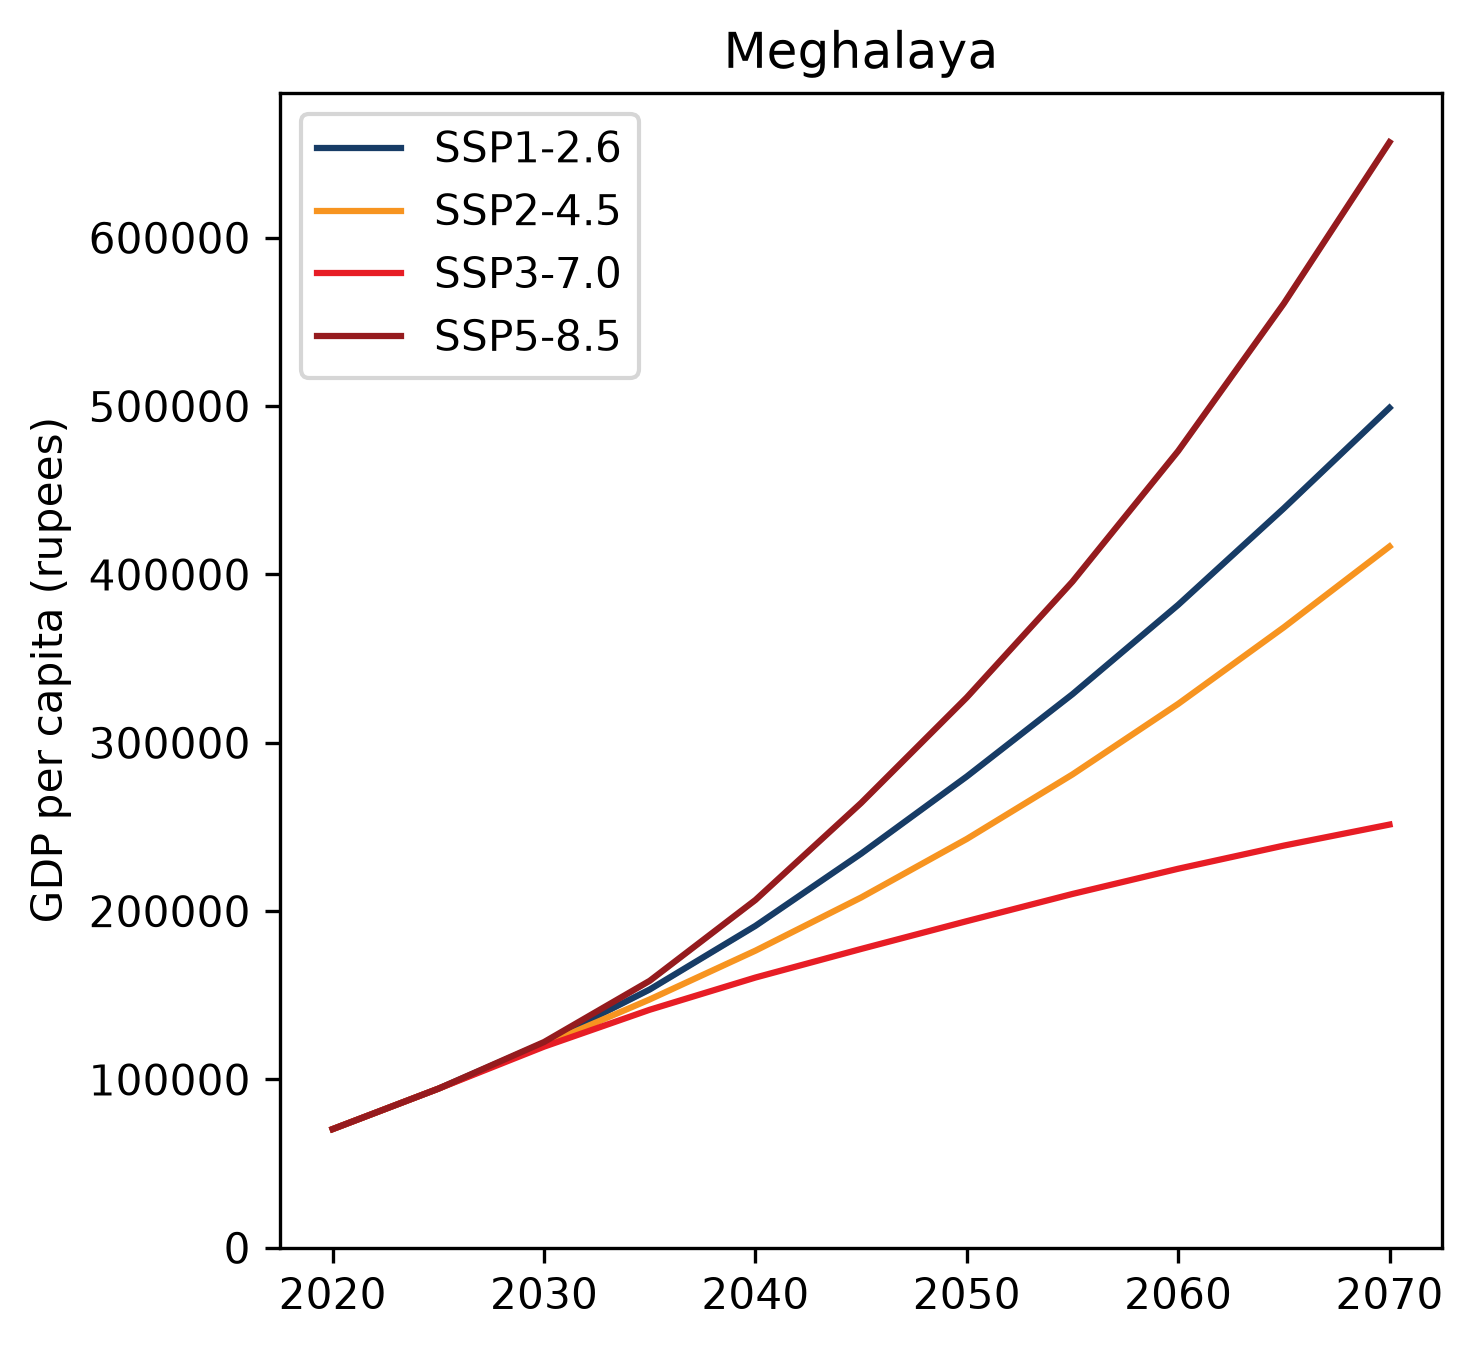
\includegraphics[height=0.25\textheight]{figures/projection_states/projection_gdp_per_capita_Meghalaya.png}\\
   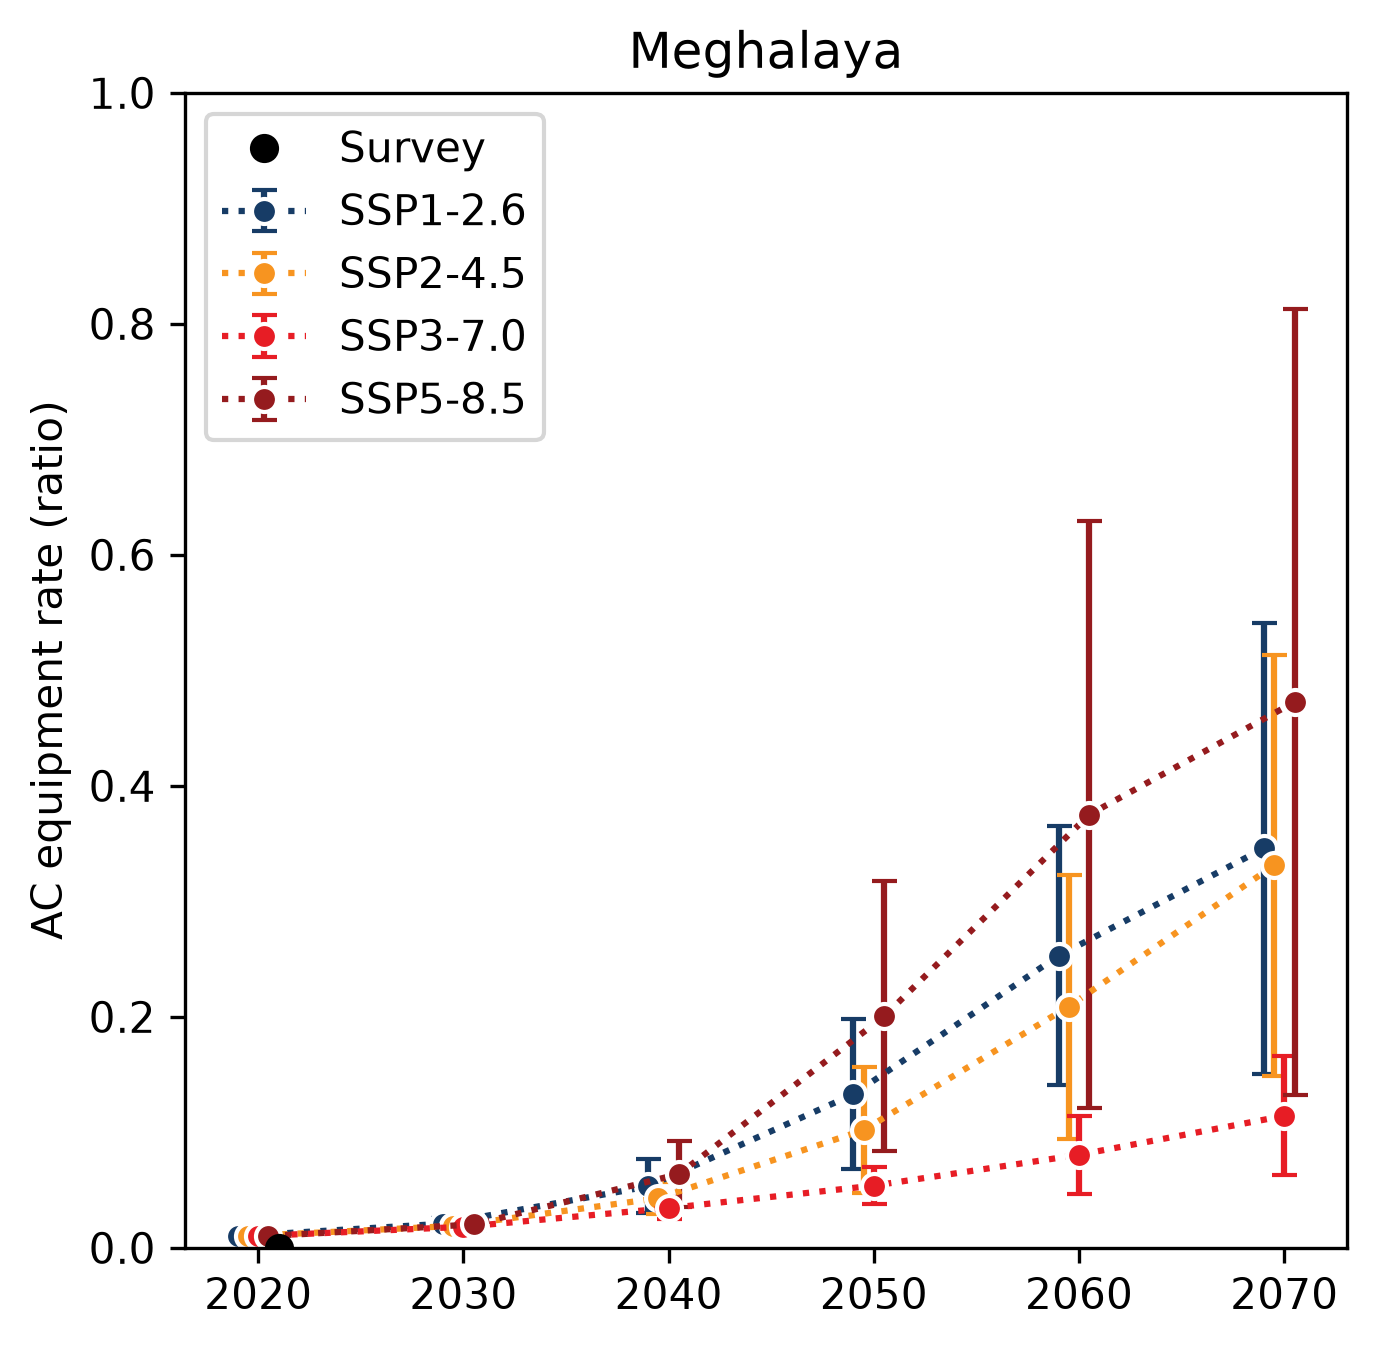
\includegraphics[height=0.25\textheight]{figures/projection_states/projection_ac_rate_Meghalaya.png}\hfill
   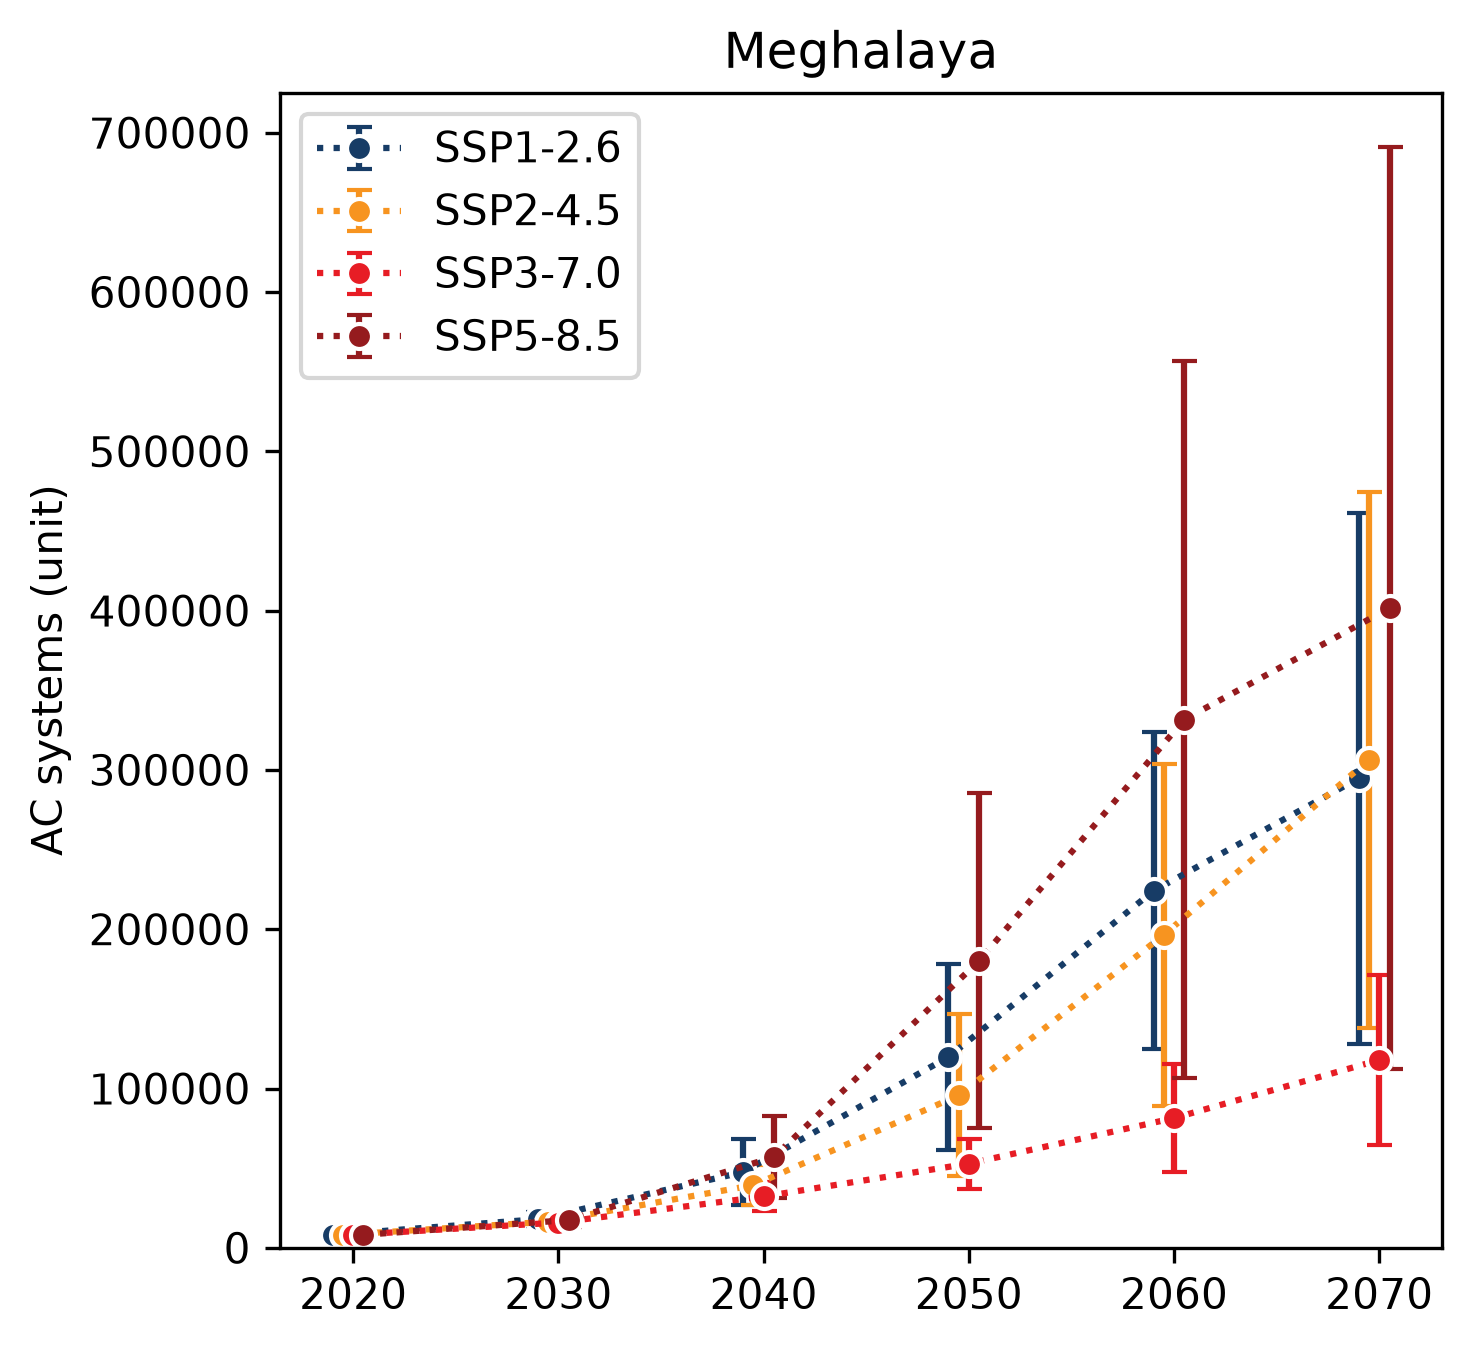
\includegraphics[height=0.25\textheight]{figures/projection_states/projection_ac_systems_Meghalaya.png}
   \caption{Projections des différentes variables pour Meghalaya}
\end{figure}

\clearpage

\subsubsection{Mizoram}

\begin{figure}[ht]
   \centering
   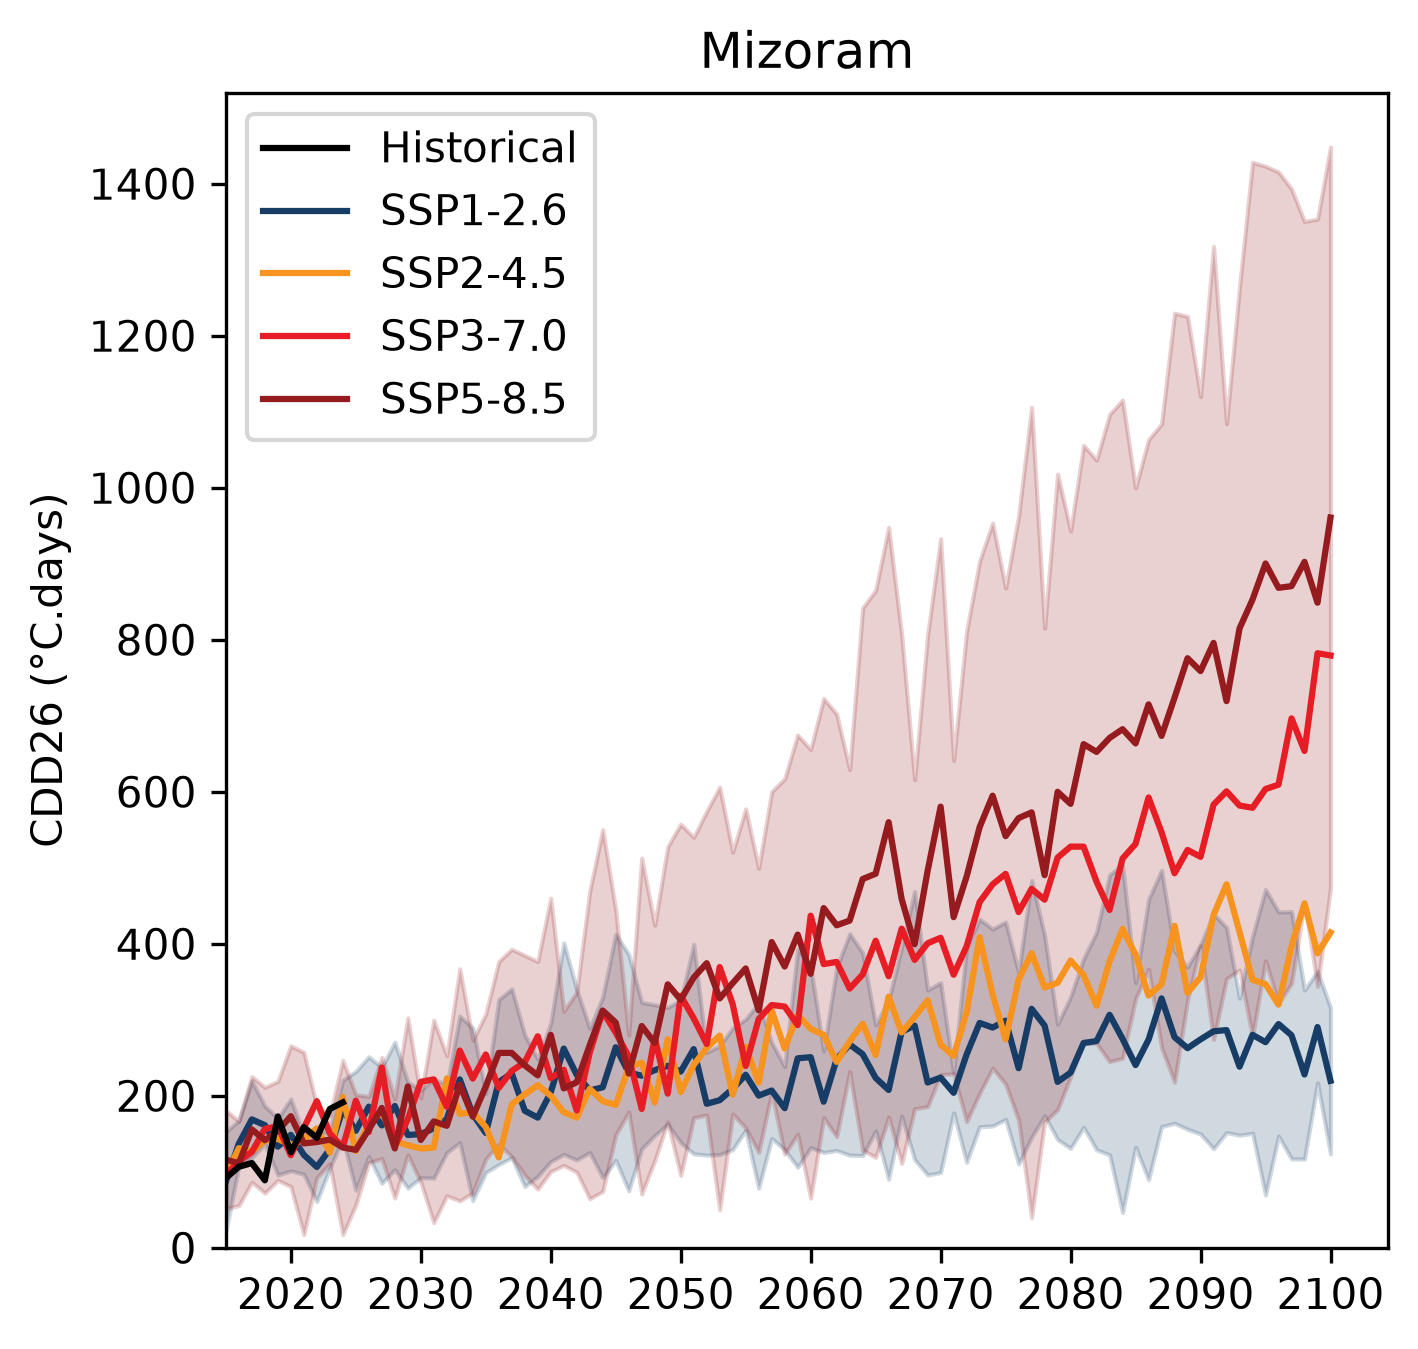
\includegraphics[height=0.25\textheight]{figures/projection_states/projection_cdd26_Mizoram.png}\hfill
   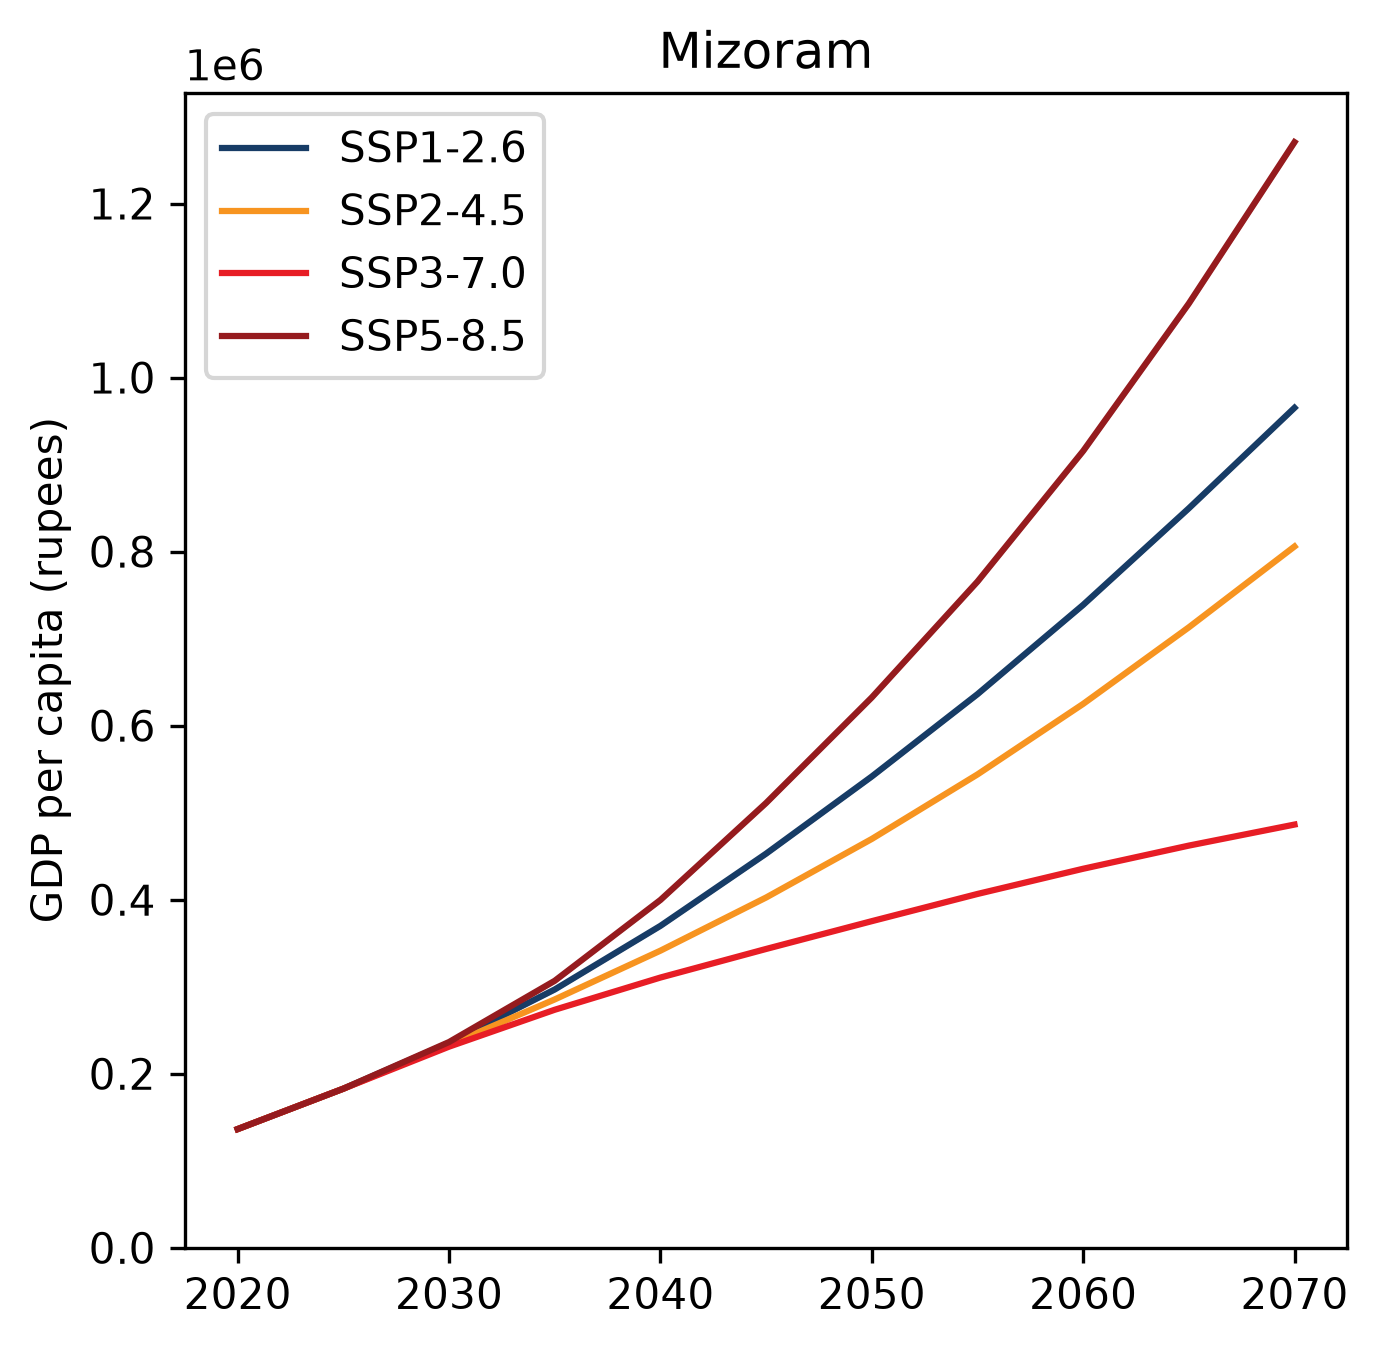
\includegraphics[height=0.25\textheight]{figures/projection_states/projection_gdp_per_capita_Mizoram.png}\\
   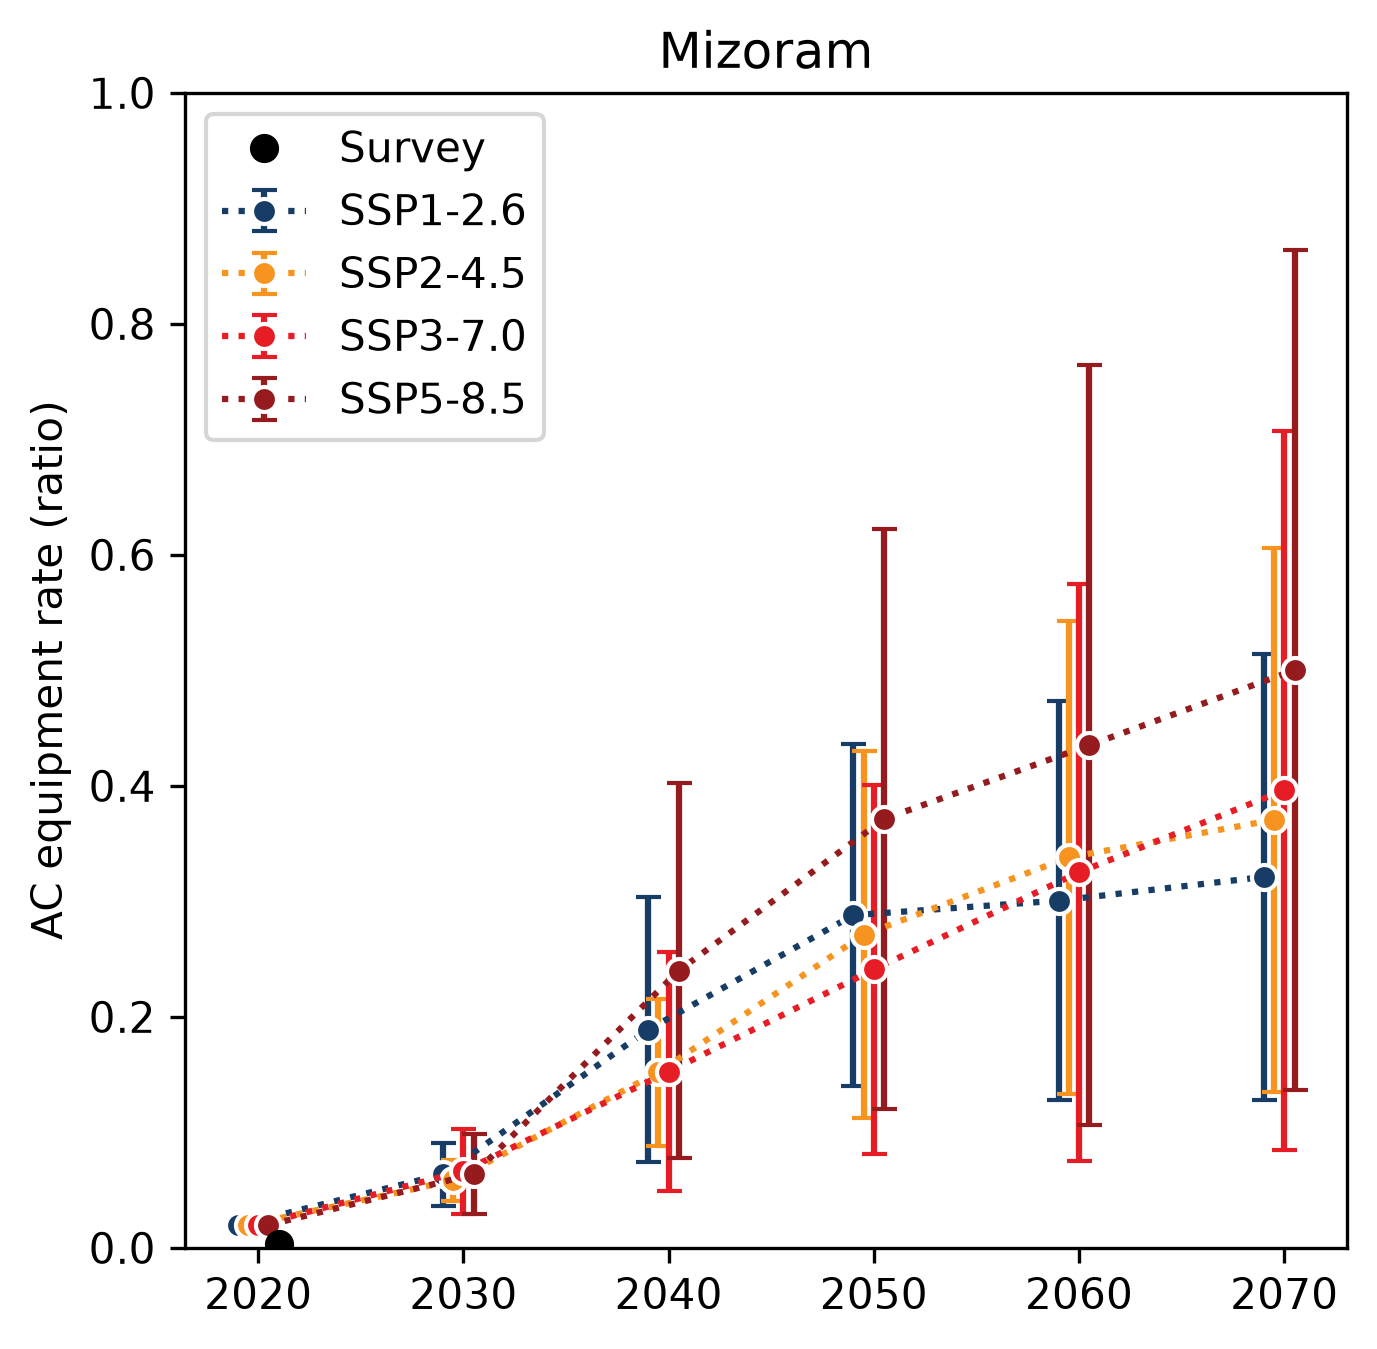
\includegraphics[height=0.25\textheight]{figures/projection_states/projection_ac_rate_Mizoram.png}\hfill
   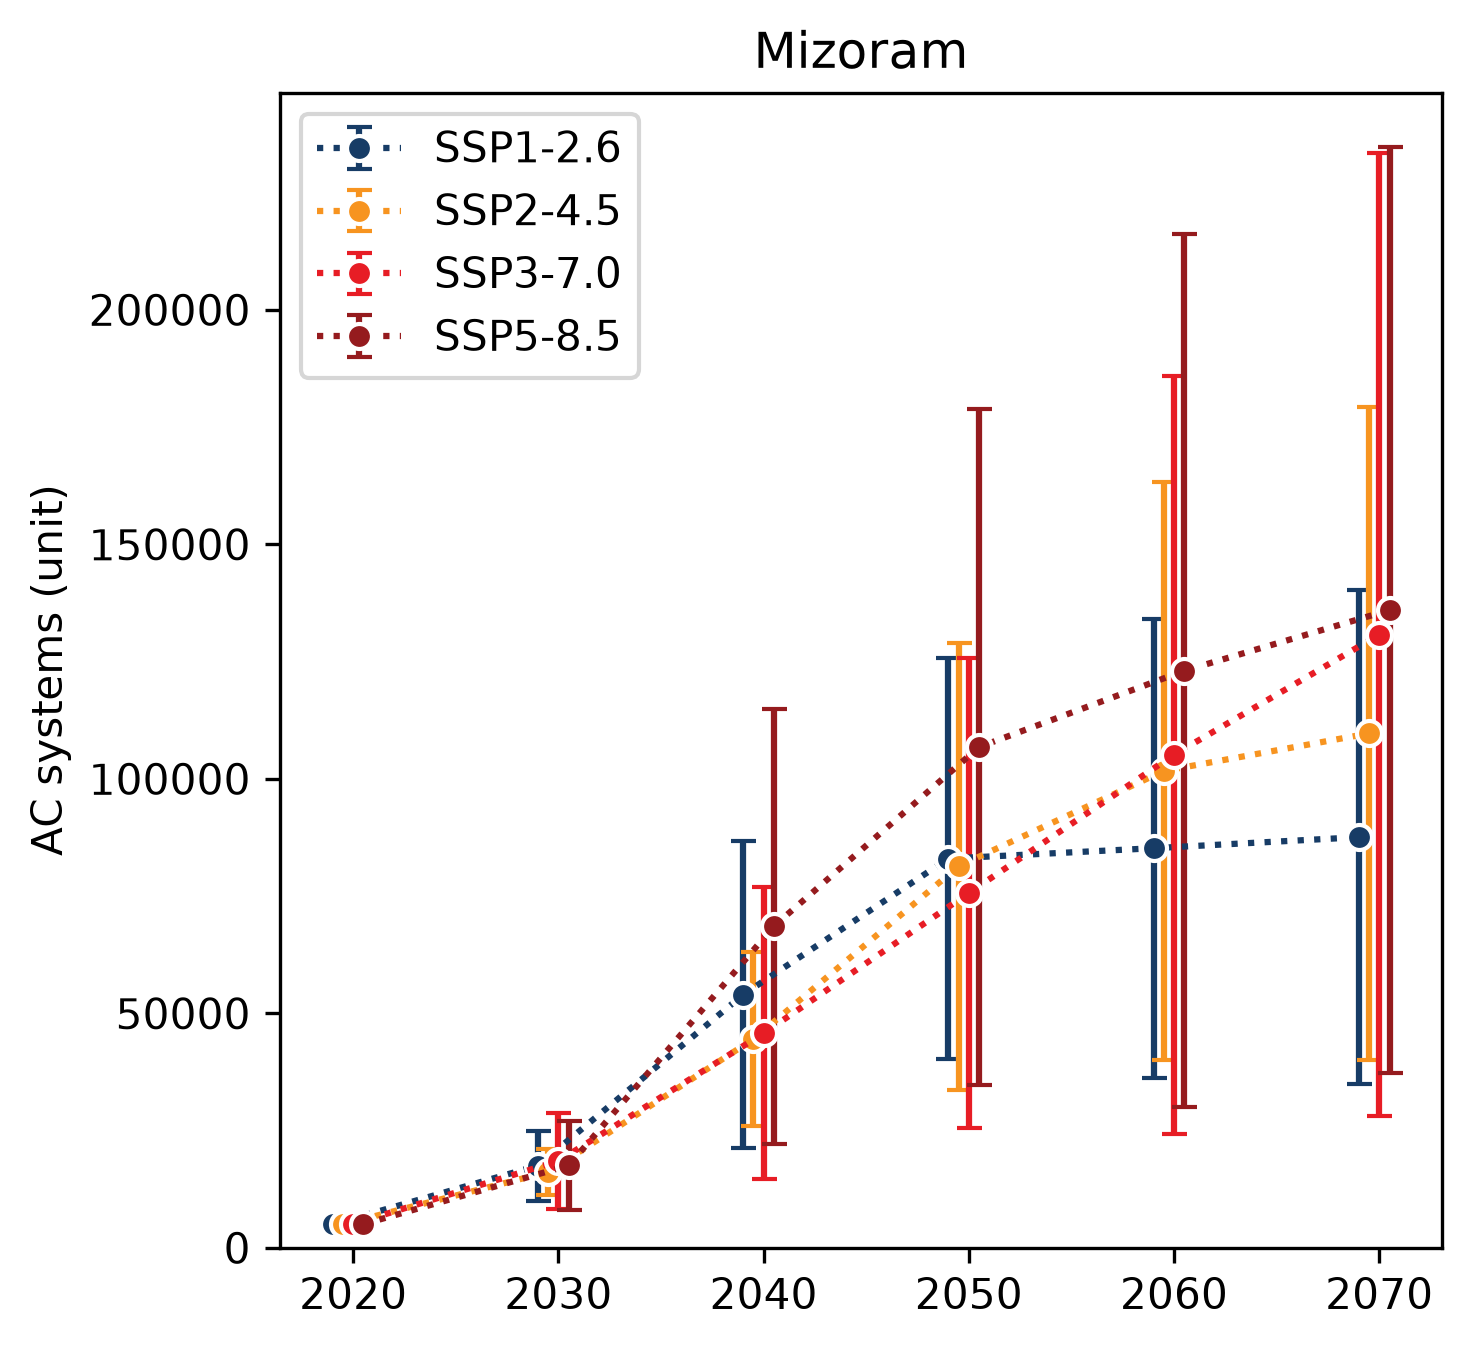
\includegraphics[height=0.25\textheight]{figures/projection_states/projection_ac_systems_Mizoram.png}
   \caption{Projections des différentes variables pour Mizoram}
\end{figure}

\clearpage

\subsubsection{Nagaland}

\begin{figure}[ht]
   \centering
   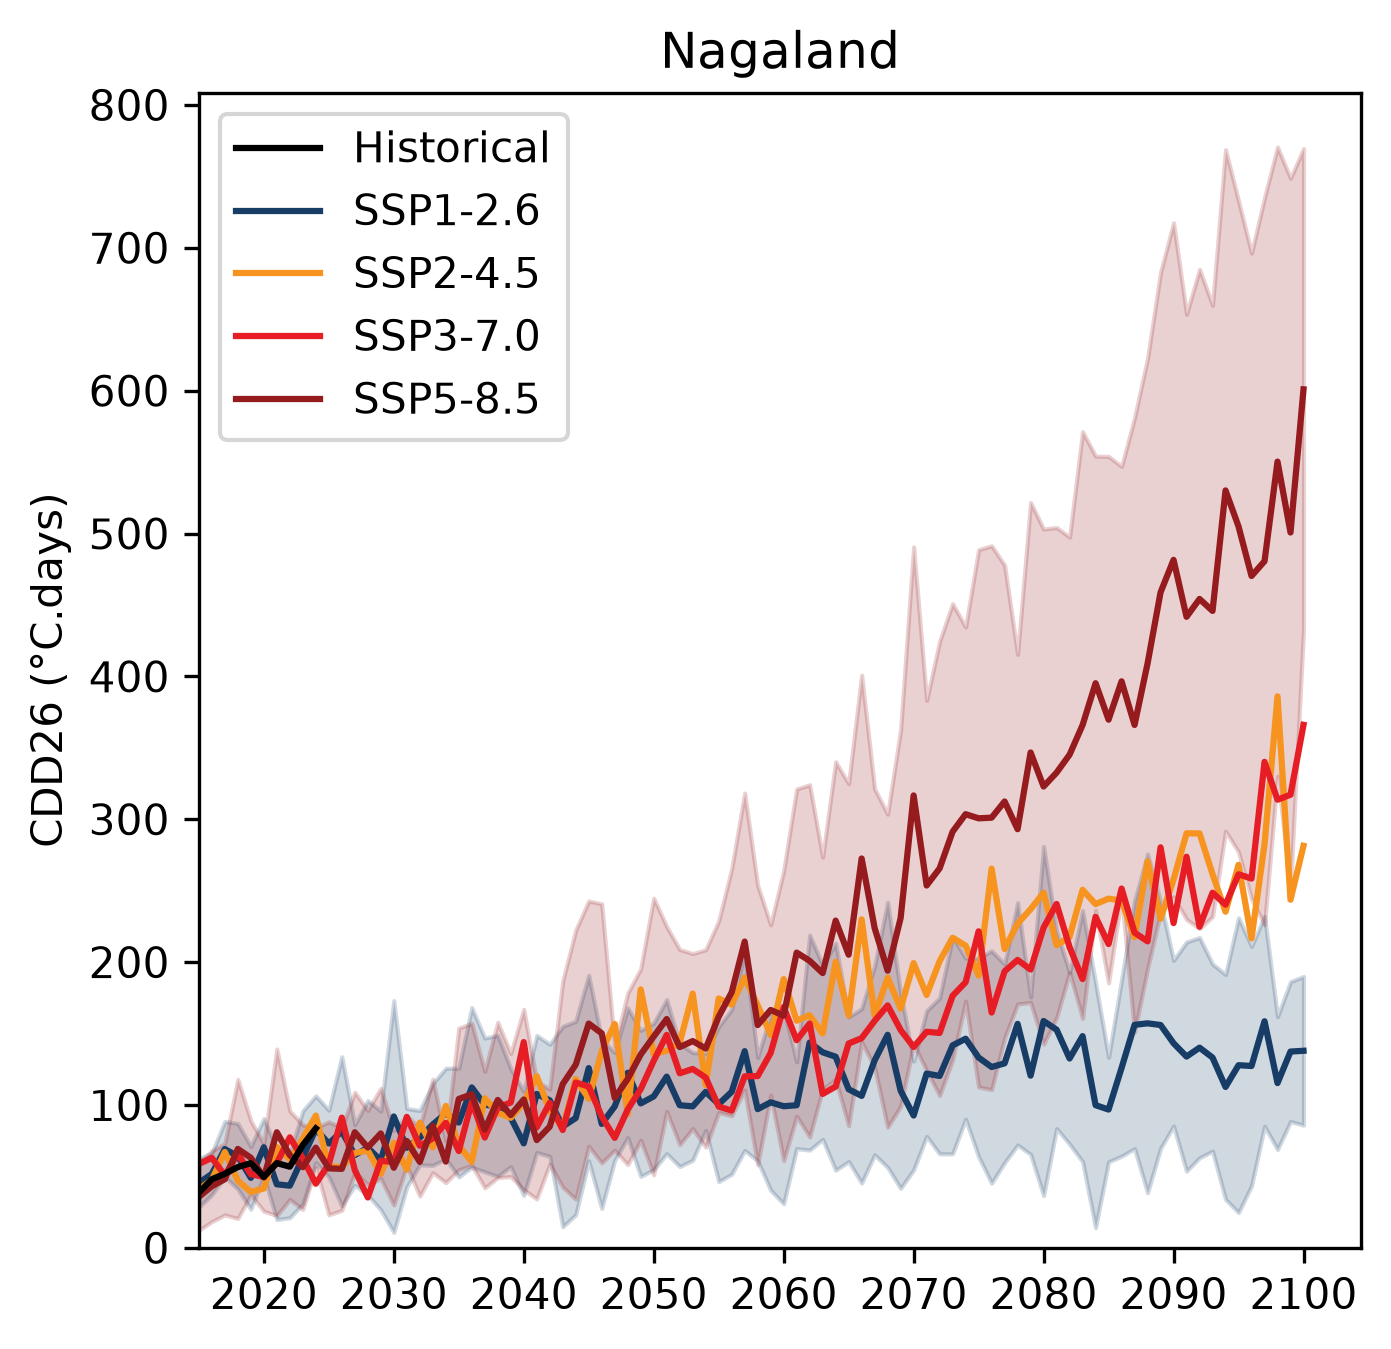
\includegraphics[height=0.25\textheight]{figures/projection_states/projection_cdd26_Nagaland.png}\hfill
   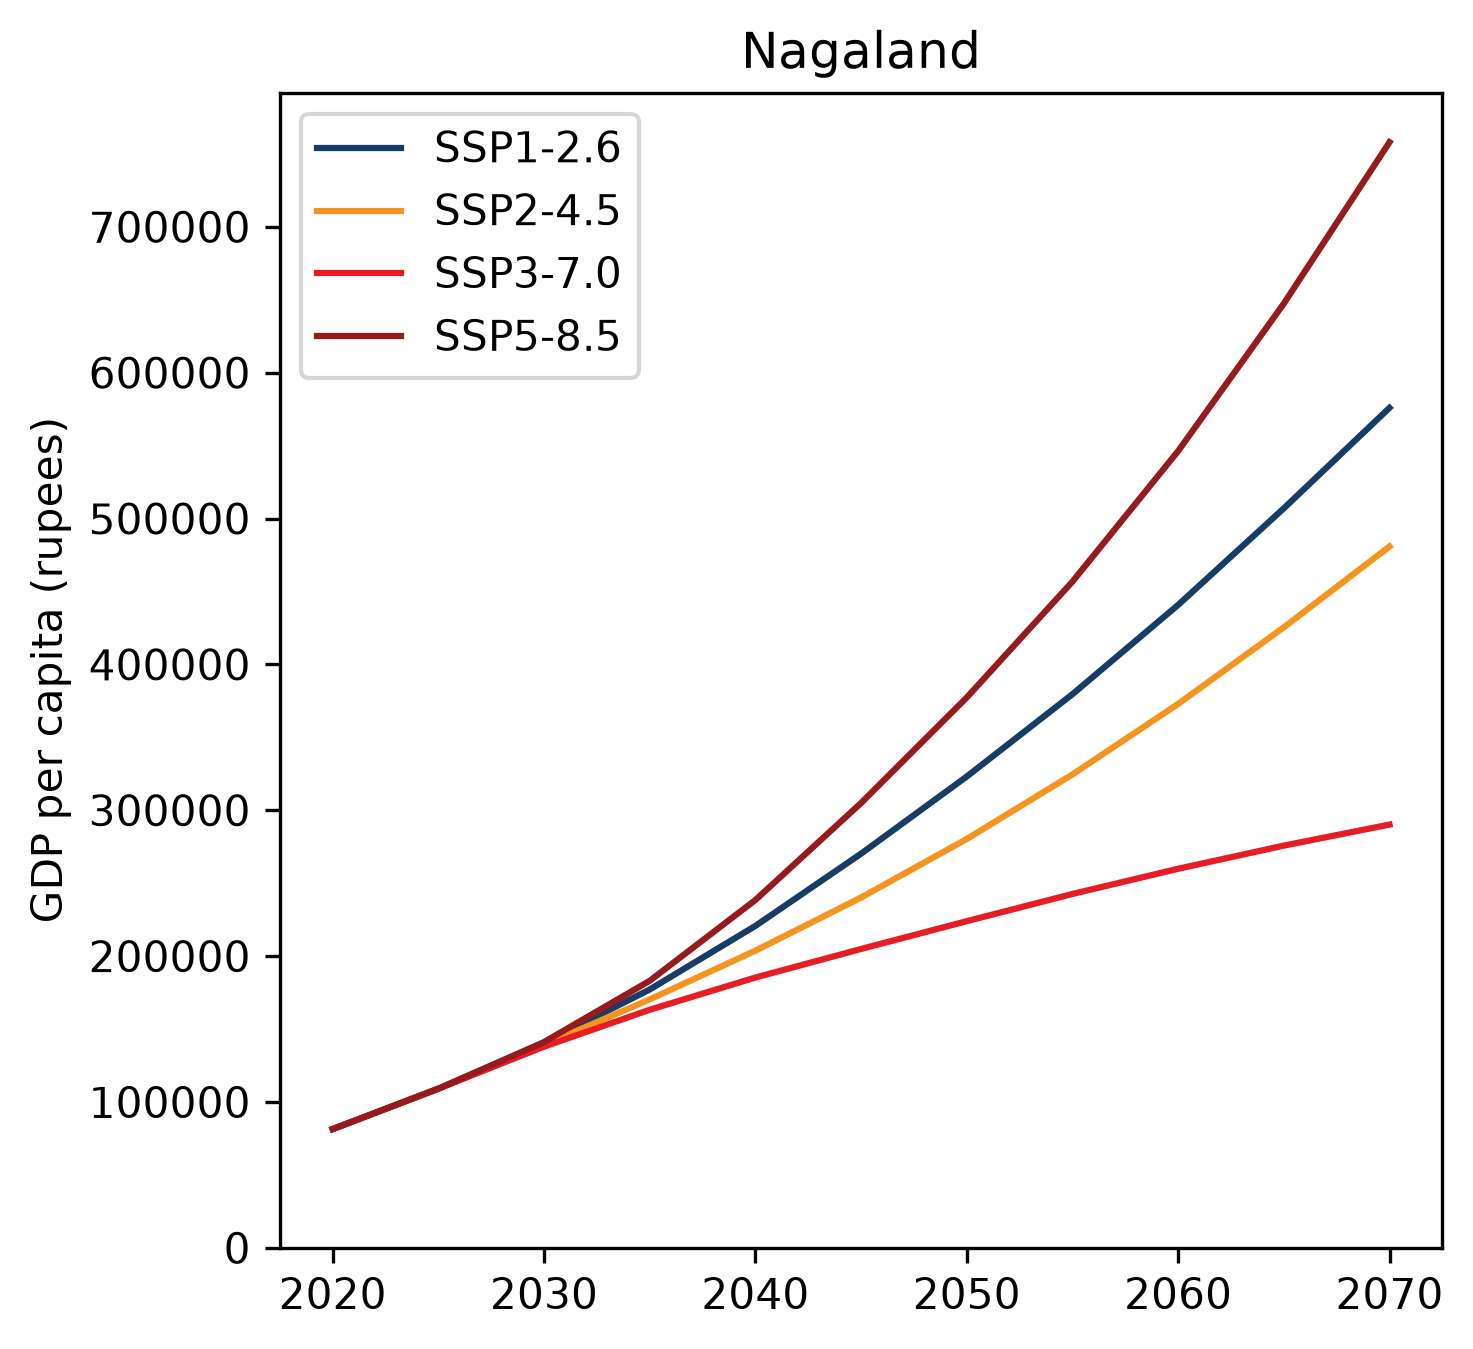
\includegraphics[height=0.25\textheight]{figures/projection_states/projection_gdp_per_capita_Nagaland.png}\\
   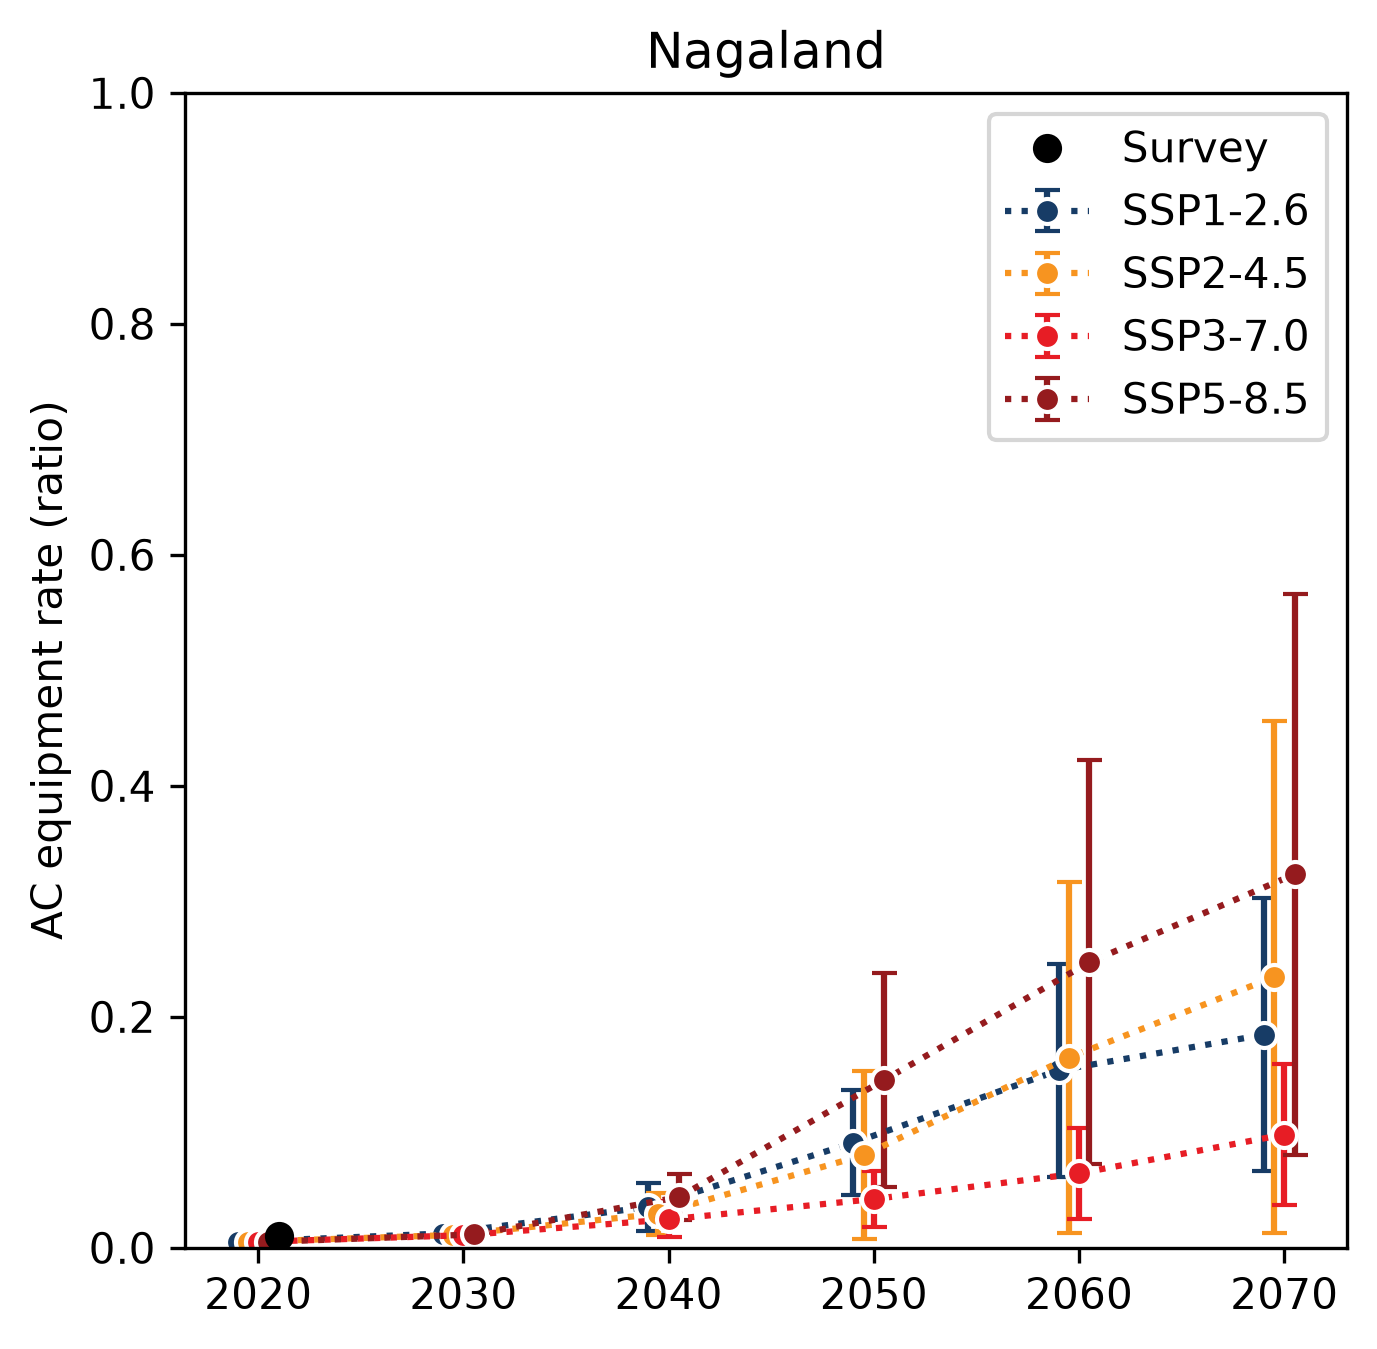
\includegraphics[height=0.25\textheight]{figures/projection_states/projection_ac_rate_Nagaland.png}\hfill
   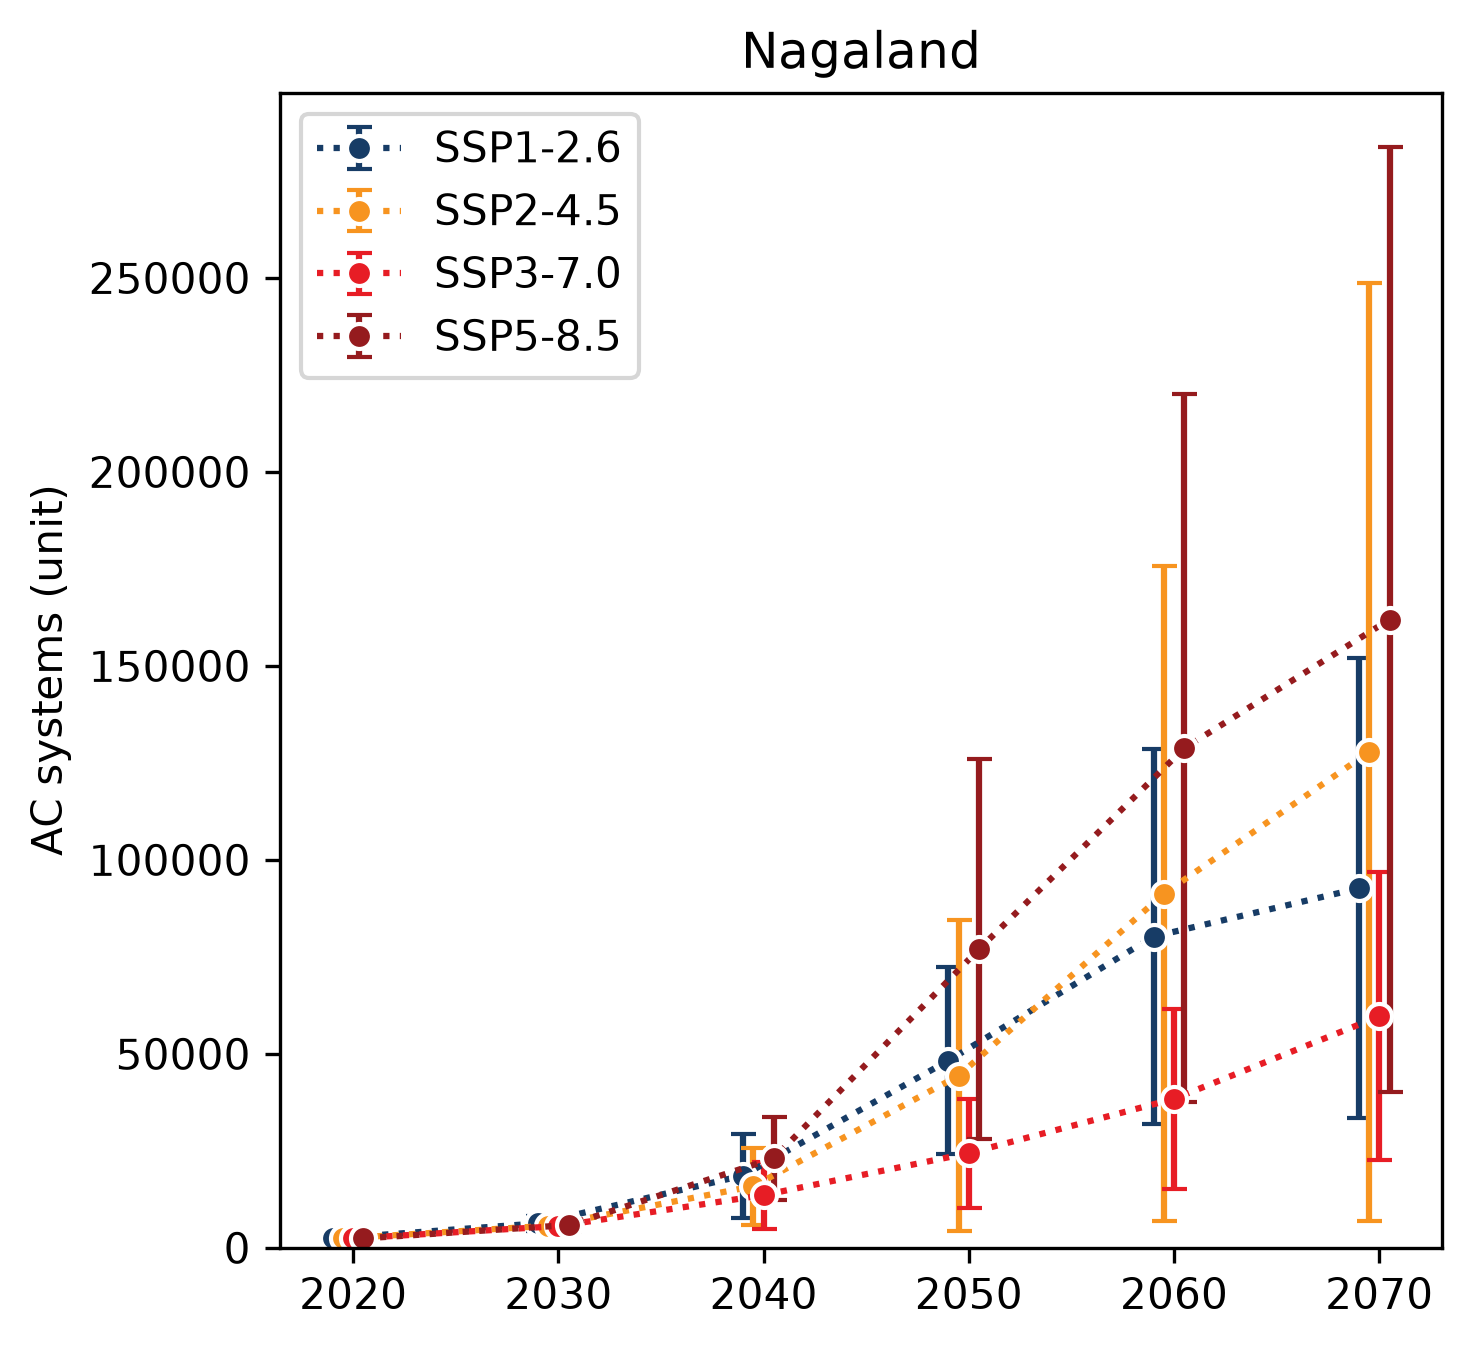
\includegraphics[height=0.25\textheight]{figures/projection_states/projection_ac_systems_Nagaland.png}
   \caption{Projections des différentes variables pour Nagaland}
\end{figure}

\clearpage

\subsubsection{Odisha}

\begin{figure}[ht]
   \centering
   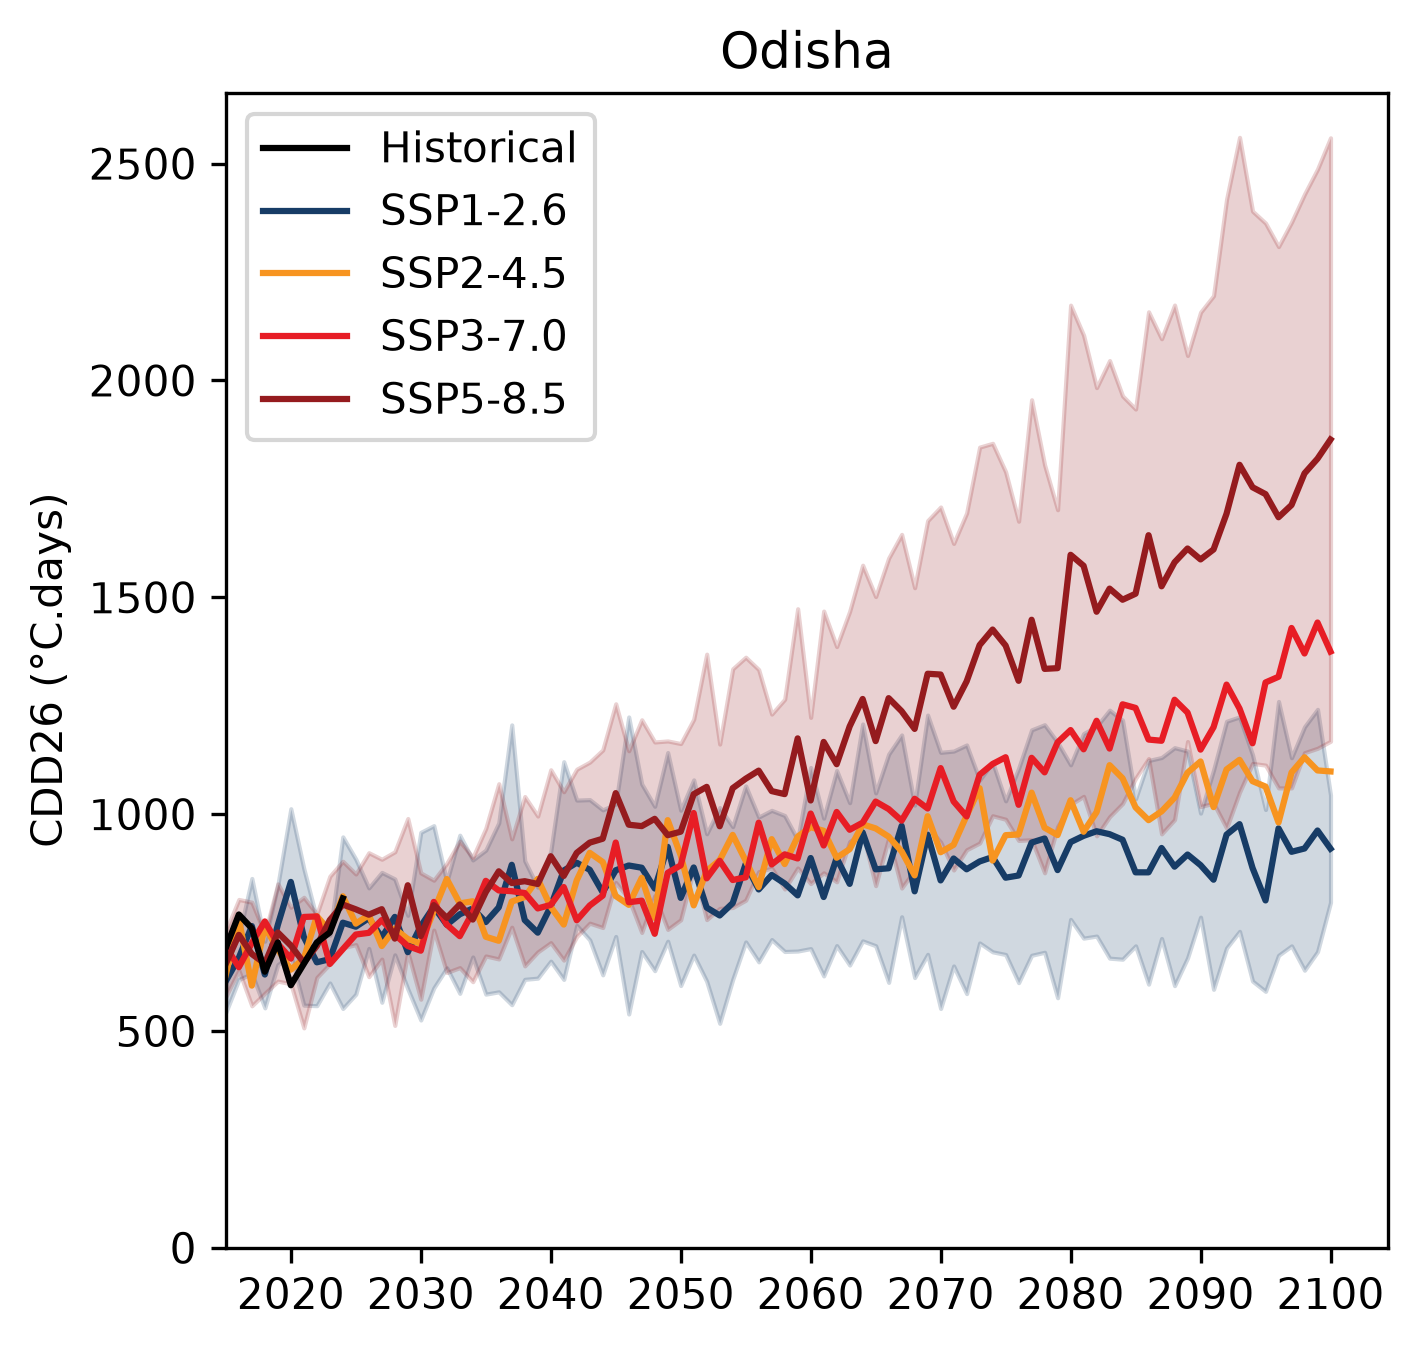
\includegraphics[height=0.25\textheight]{figures/projection_states/projection_cdd26_Odisha.png}\hfill
   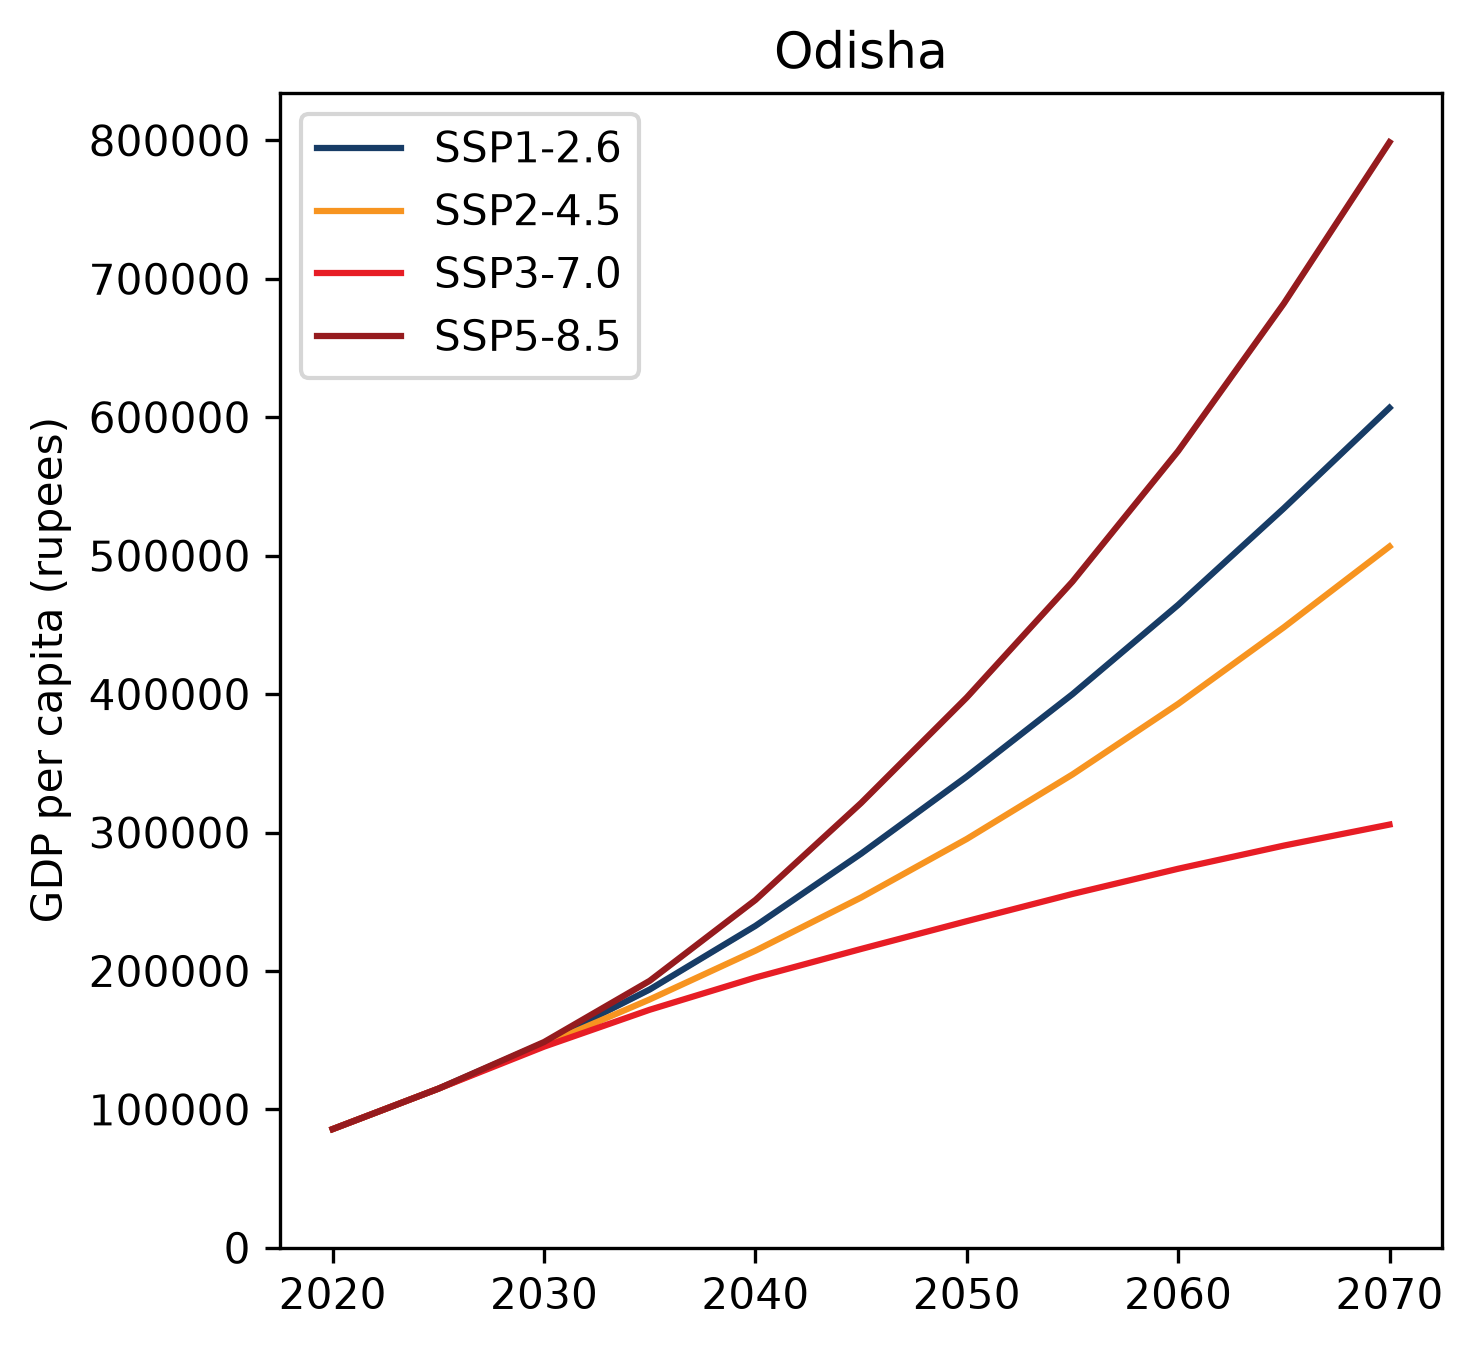
\includegraphics[height=0.25\textheight]{figures/projection_states/projection_gdp_per_capita_Odisha.png}\\
   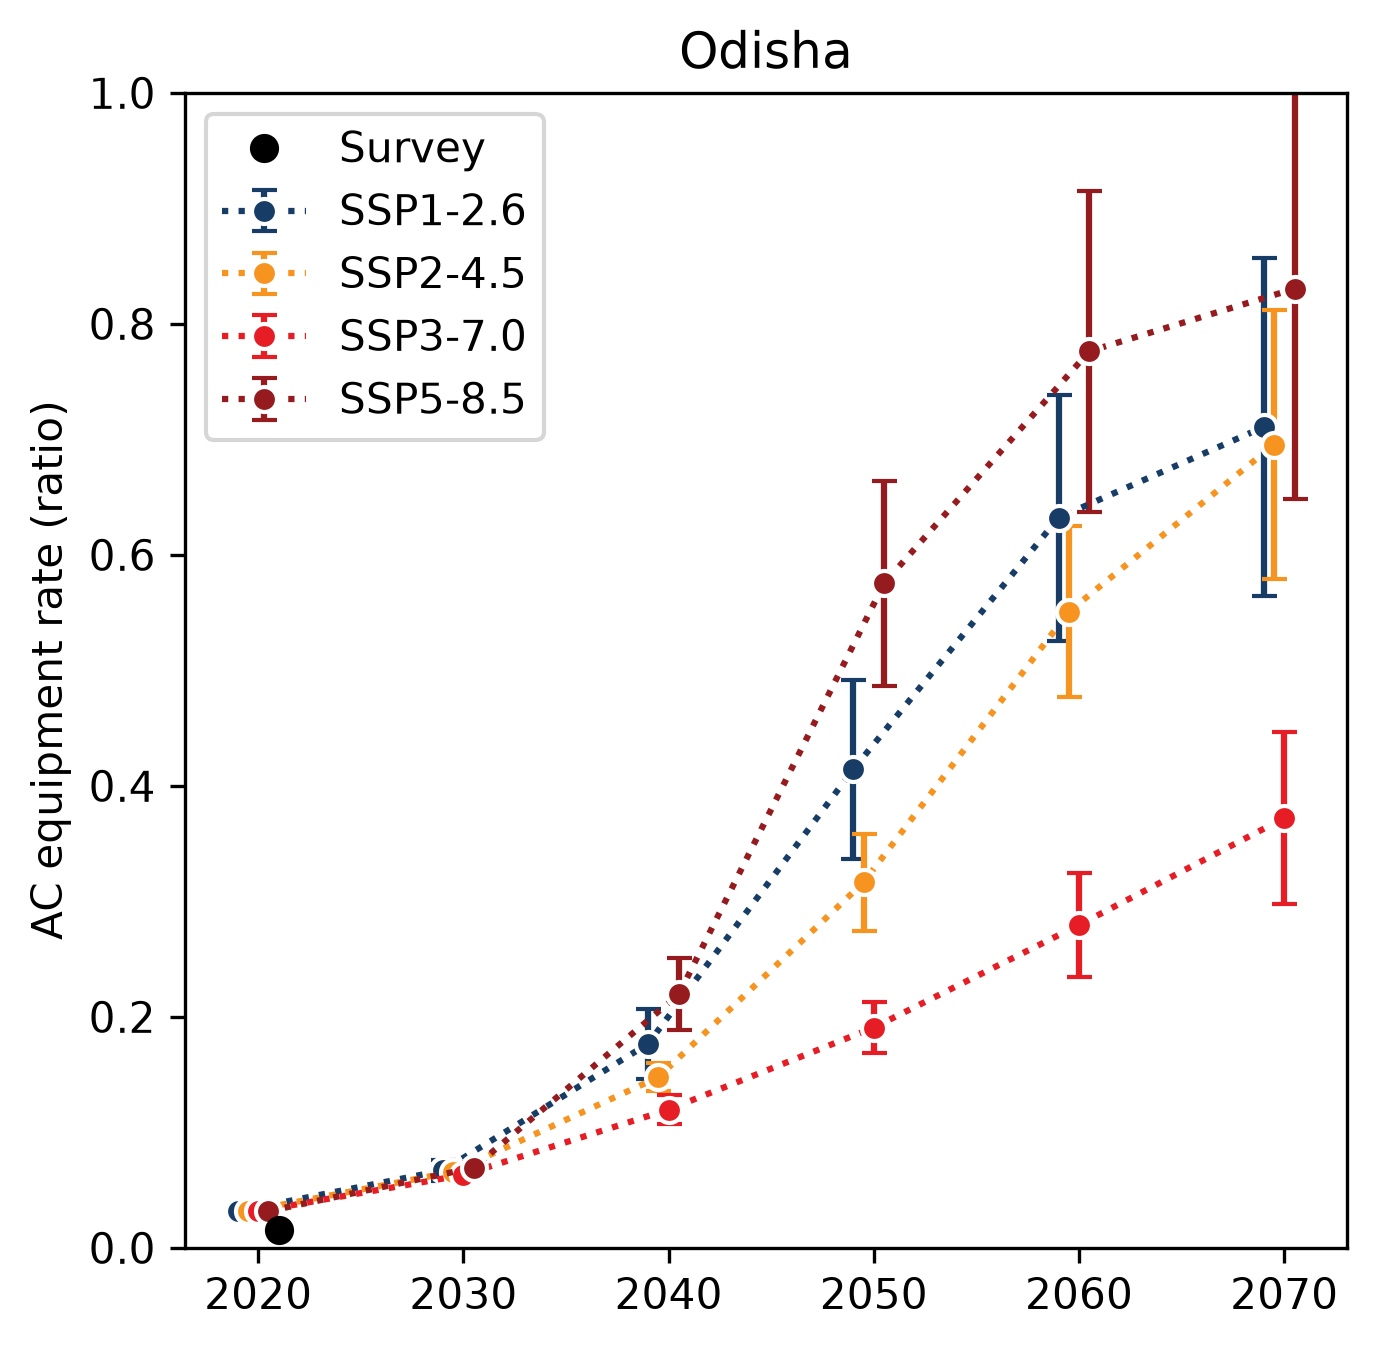
\includegraphics[height=0.25\textheight]{figures/projection_states/projection_ac_rate_Odisha.png}\hfill
   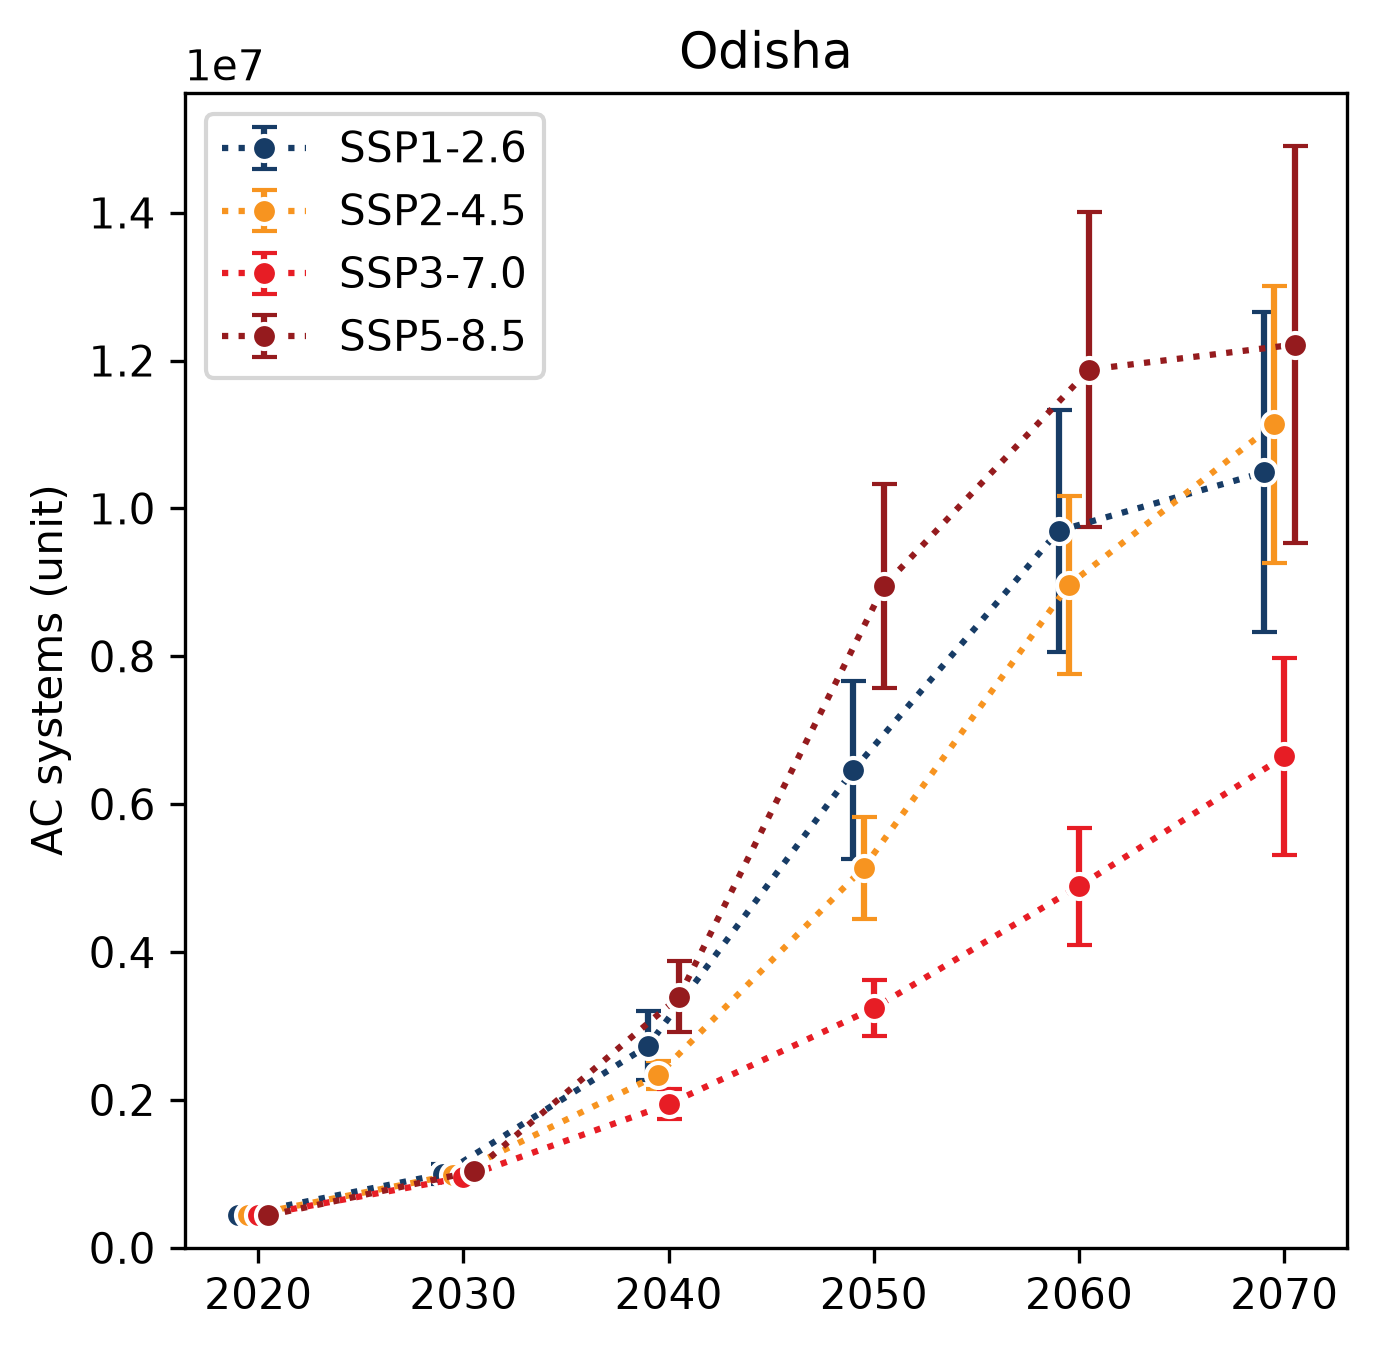
\includegraphics[height=0.25\textheight]{figures/projection_states/projection_ac_systems_Odisha.png}
   \caption{Projections des différentes variables pour Odisha}
\end{figure}

\clearpage

\subsubsection{Puducherry}

\begin{figure}[ht]
   \centering
   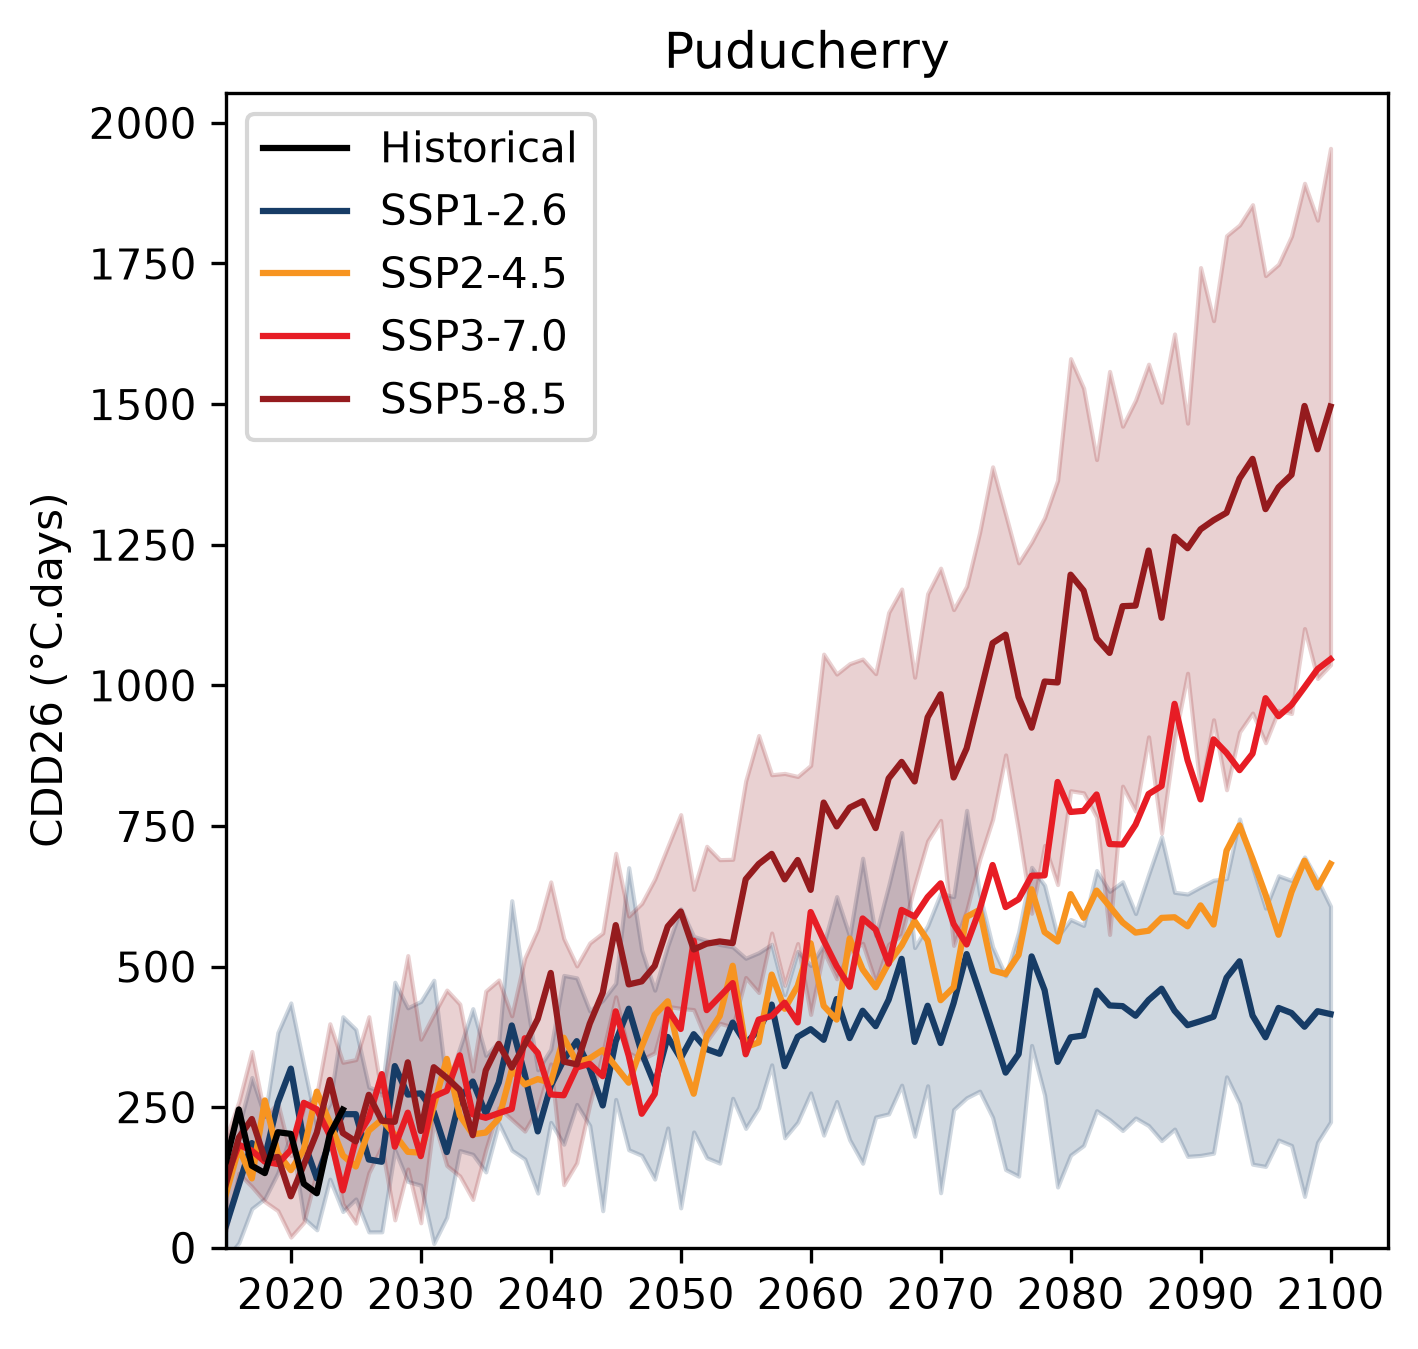
\includegraphics[height=0.25\textheight]{figures/projection_states/projection_cdd26_Puducherry.png}\hfill
   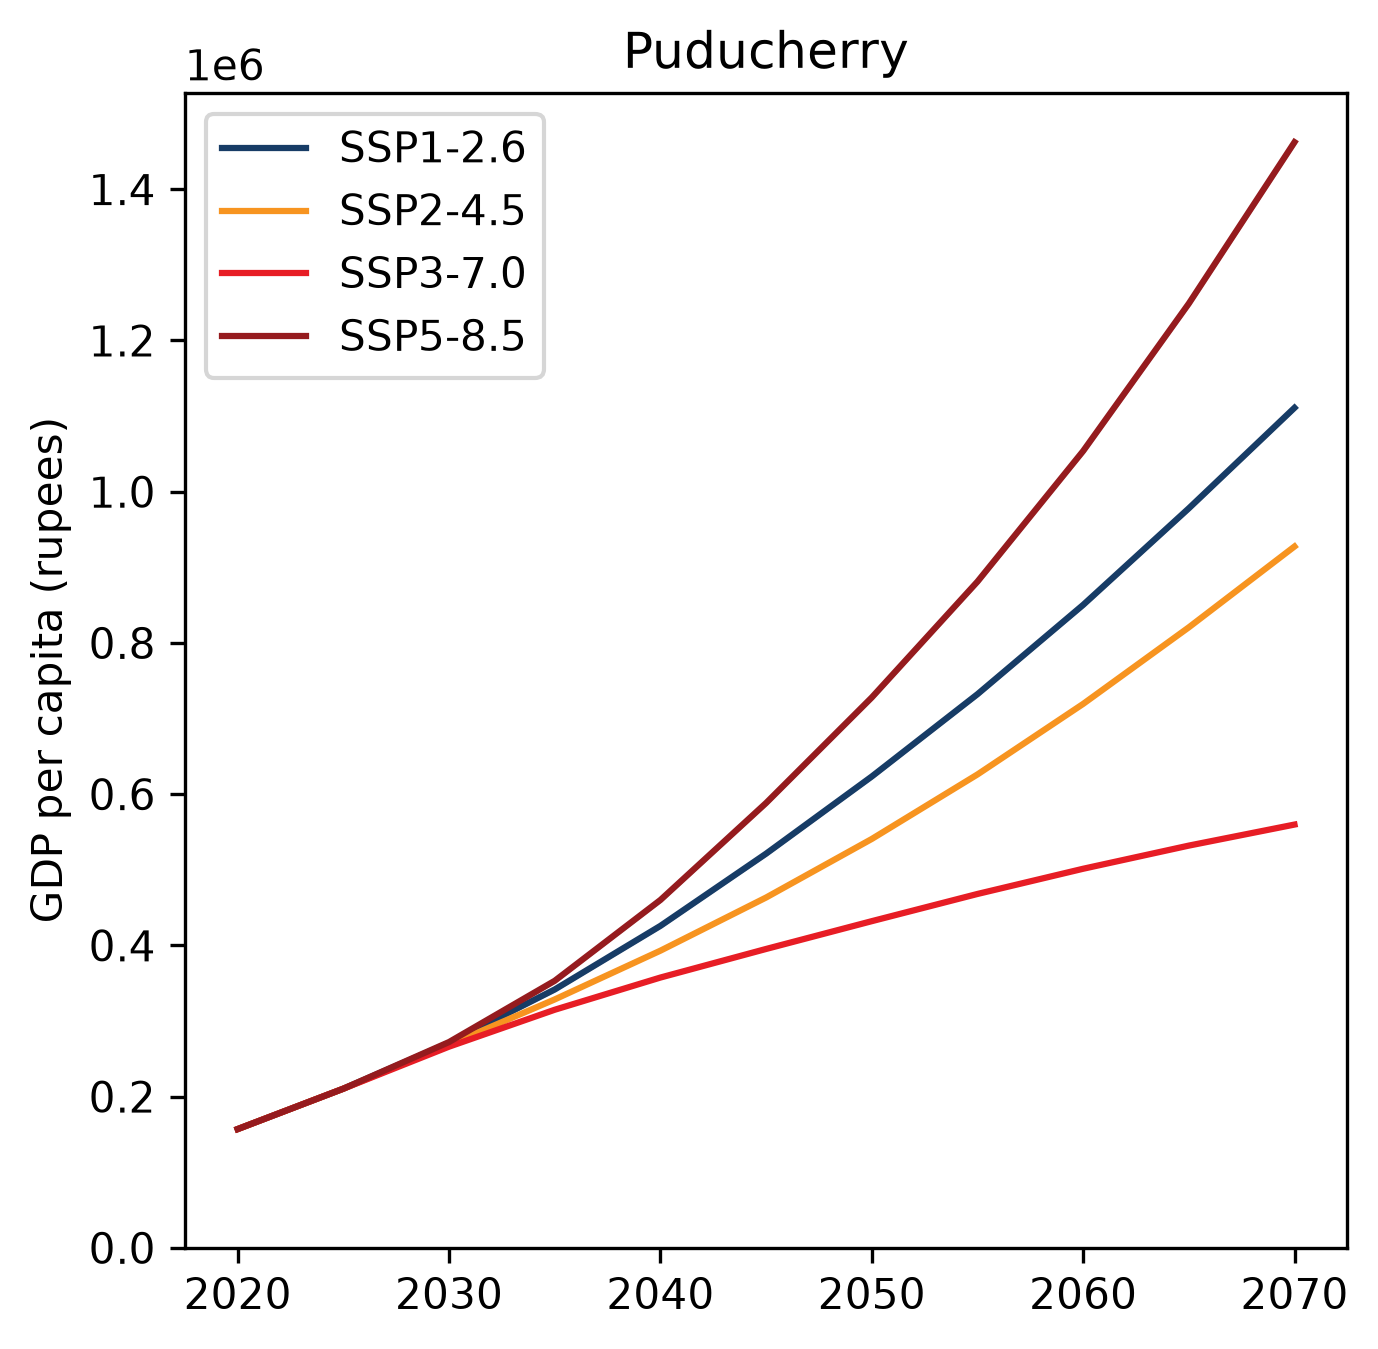
\includegraphics[height=0.25\textheight]{figures/projection_states/projection_gdp_per_capita_Puducherry.png}\\
   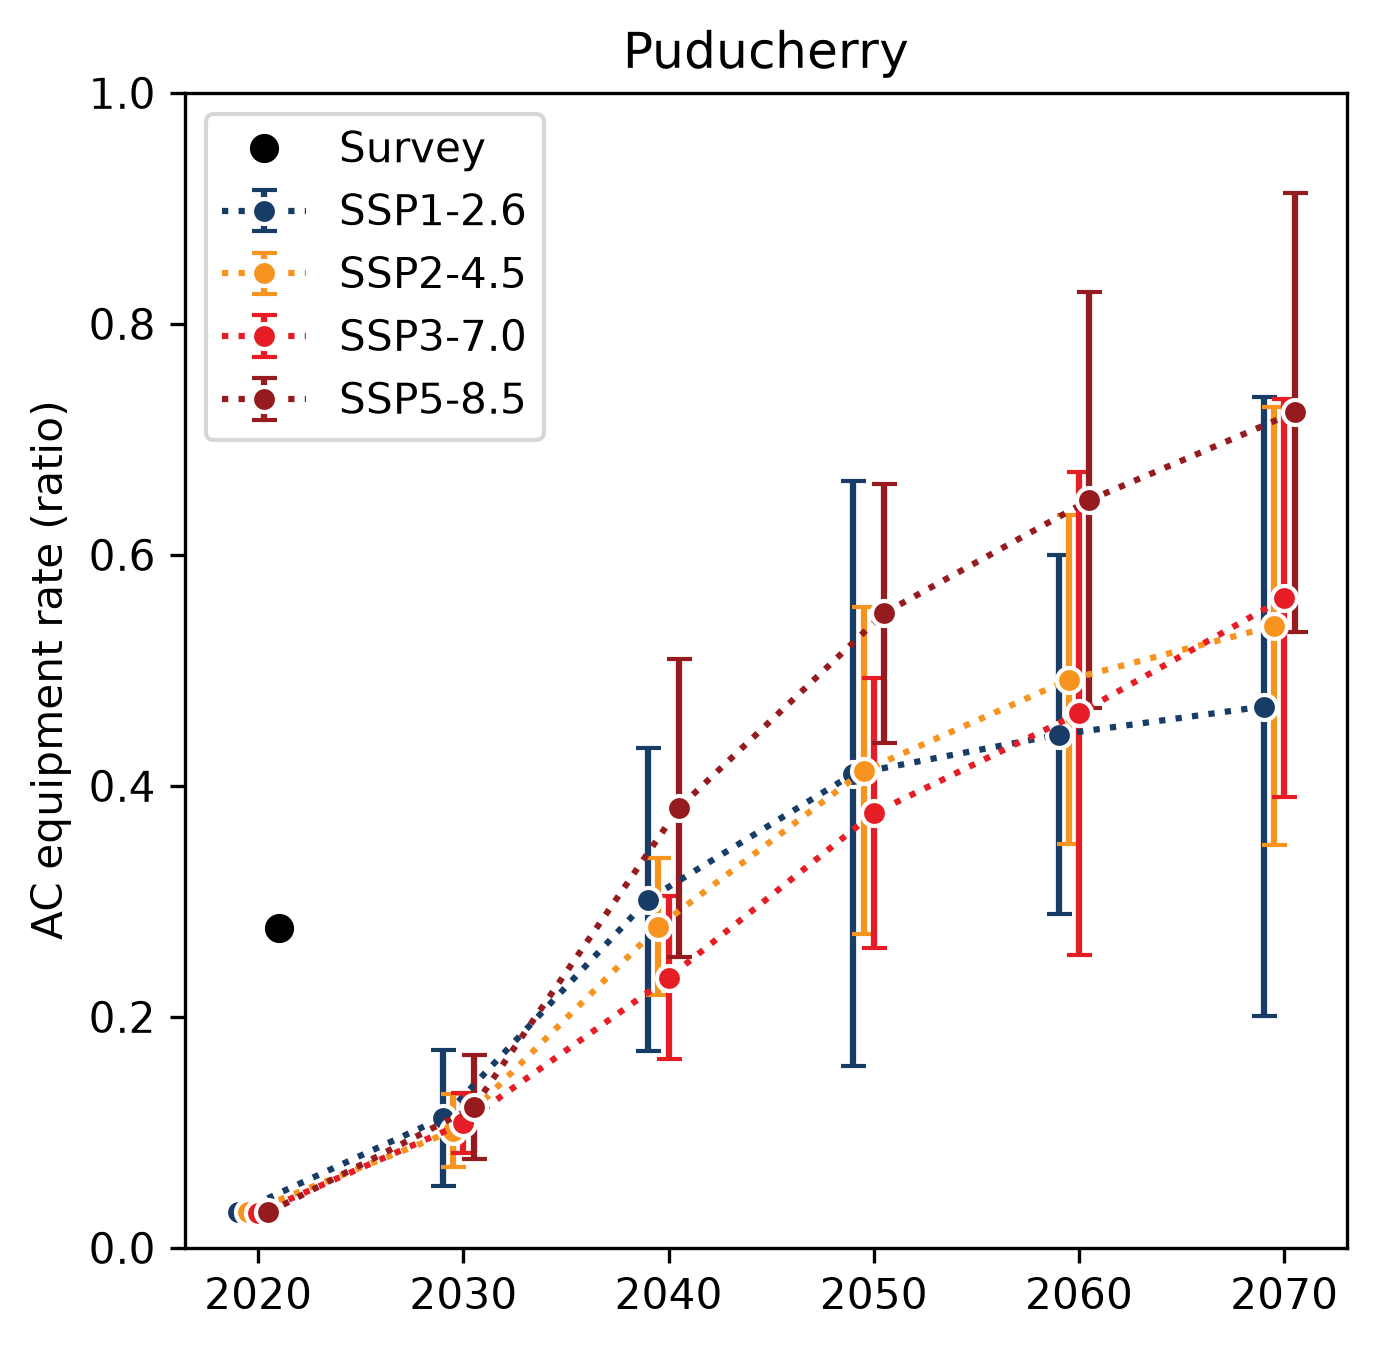
\includegraphics[height=0.25\textheight]{figures/projection_states/projection_ac_rate_Puducherry.png}\hfill
   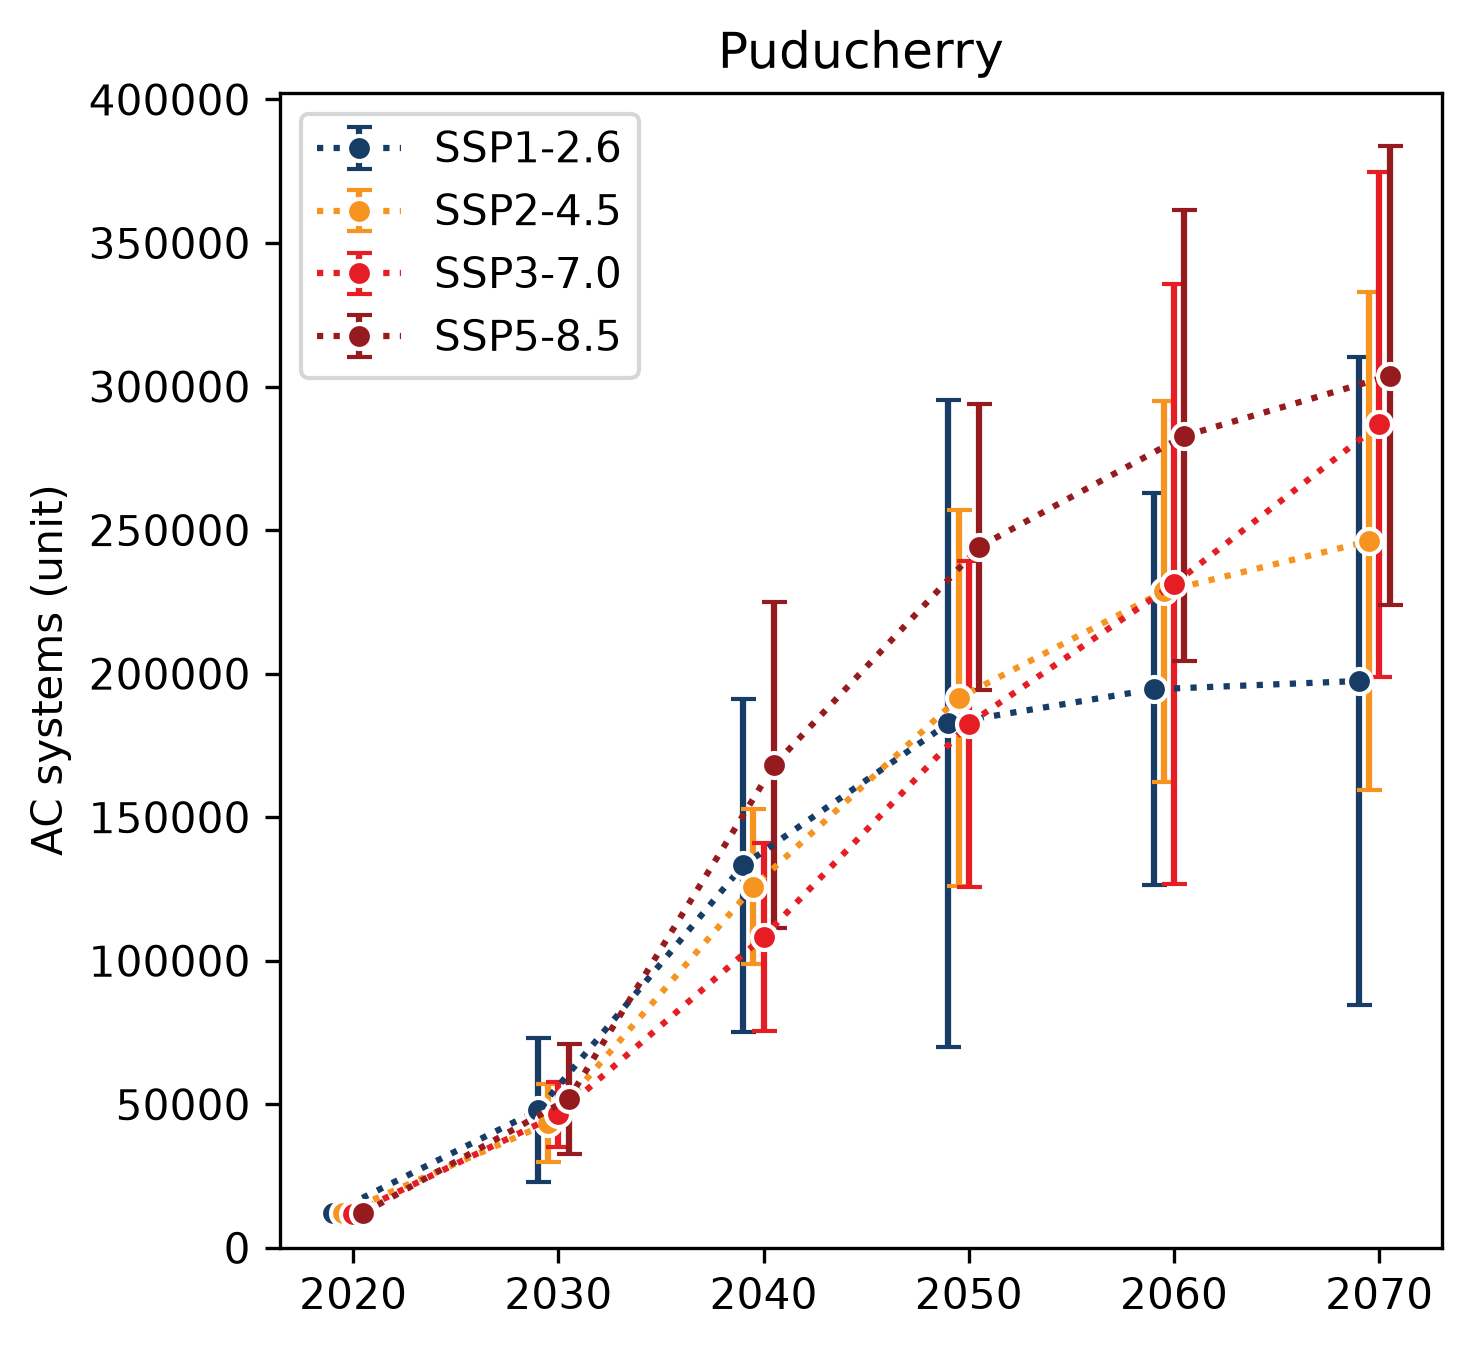
\includegraphics[height=0.25\textheight]{figures/projection_states/projection_ac_systems_Puducherry.png}
   \caption{Projections des différentes variables pour Puducherry}
\end{figure}

\clearpage

\subsubsection{Punjab}

\begin{figure}[ht]
   \centering
   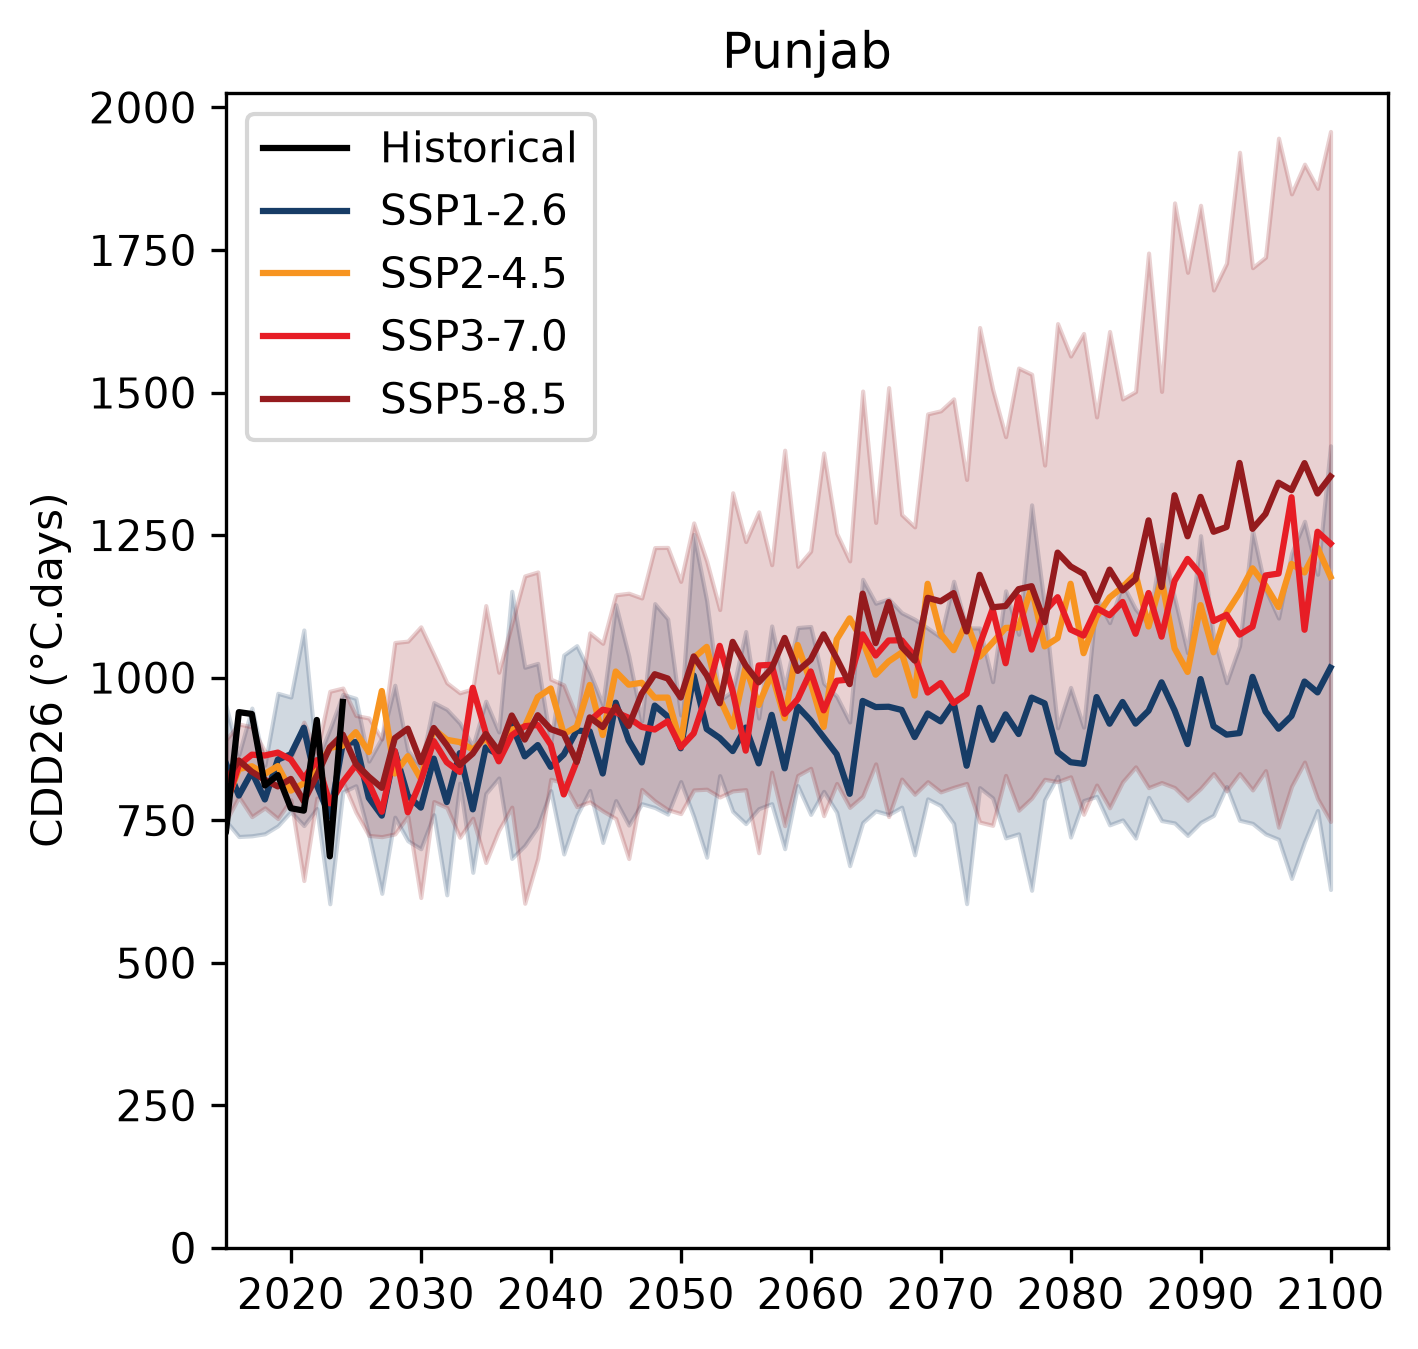
\includegraphics[height=0.25\textheight]{figures/projection_states/projection_cdd26_Punjab.png}\hfill
   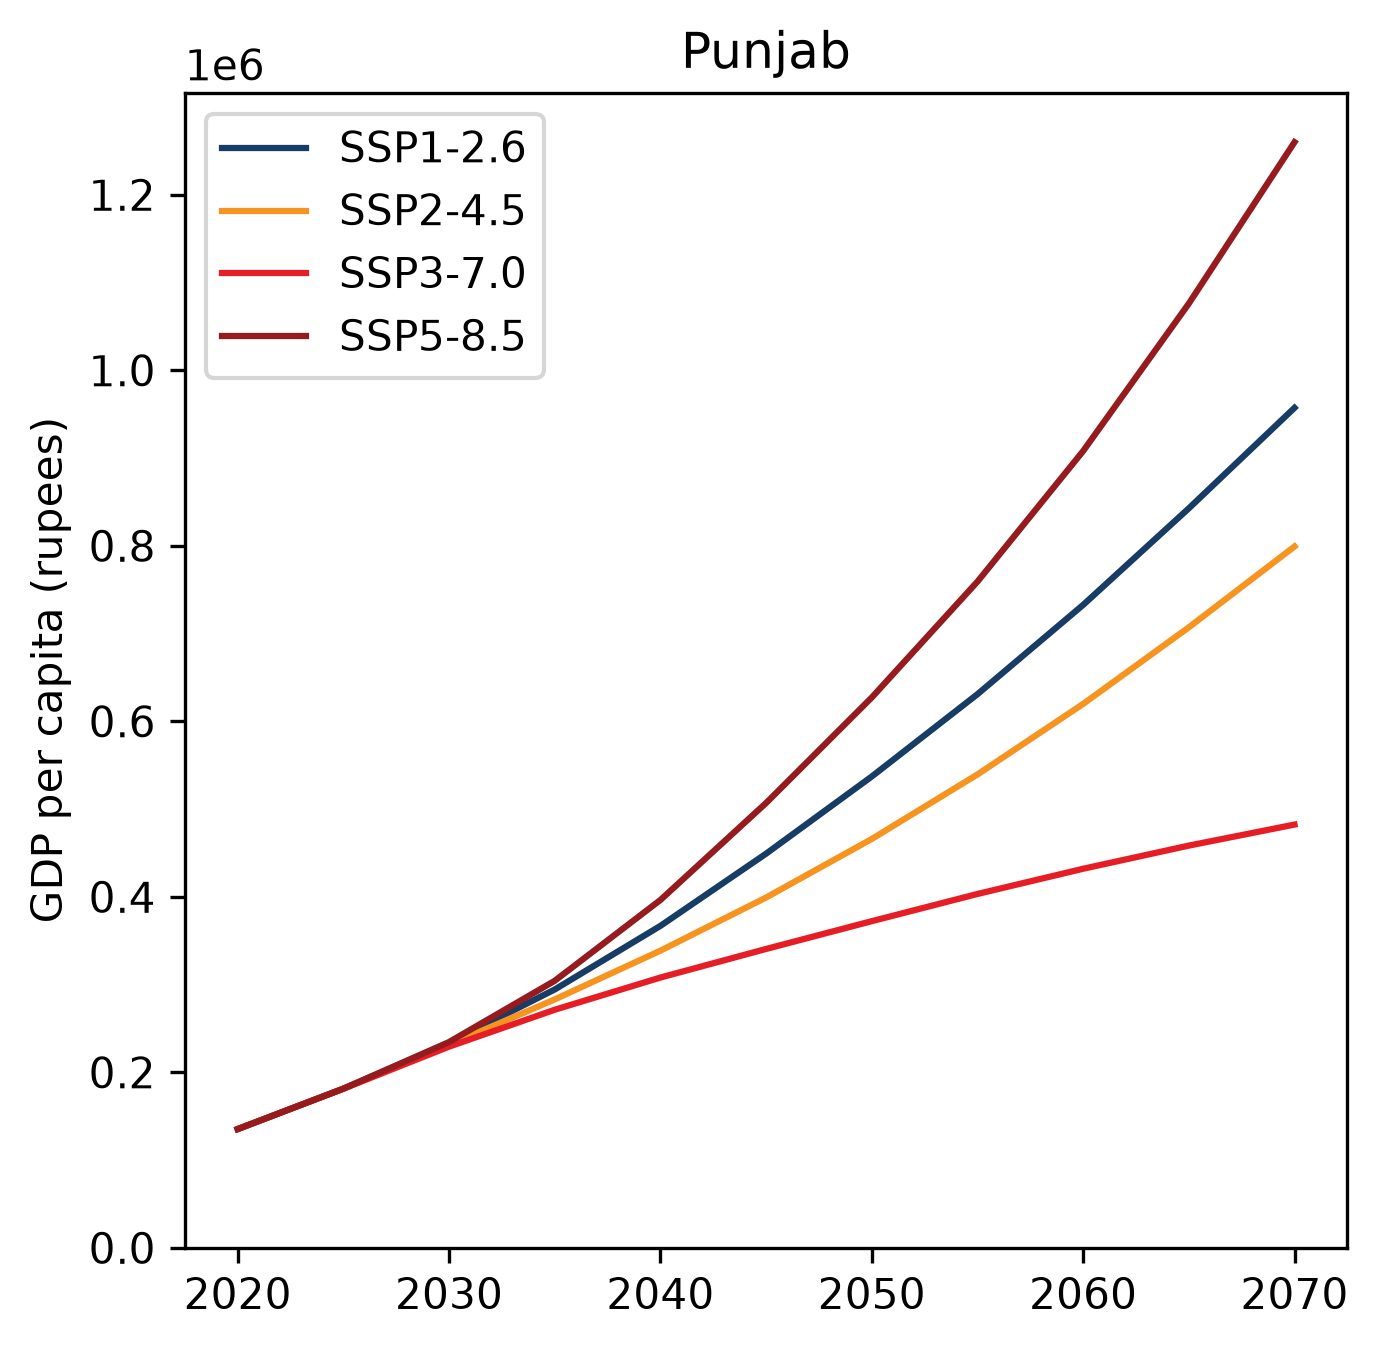
\includegraphics[height=0.25\textheight]{figures/projection_states/projection_gdp_per_capita_Punjab.png}\\
   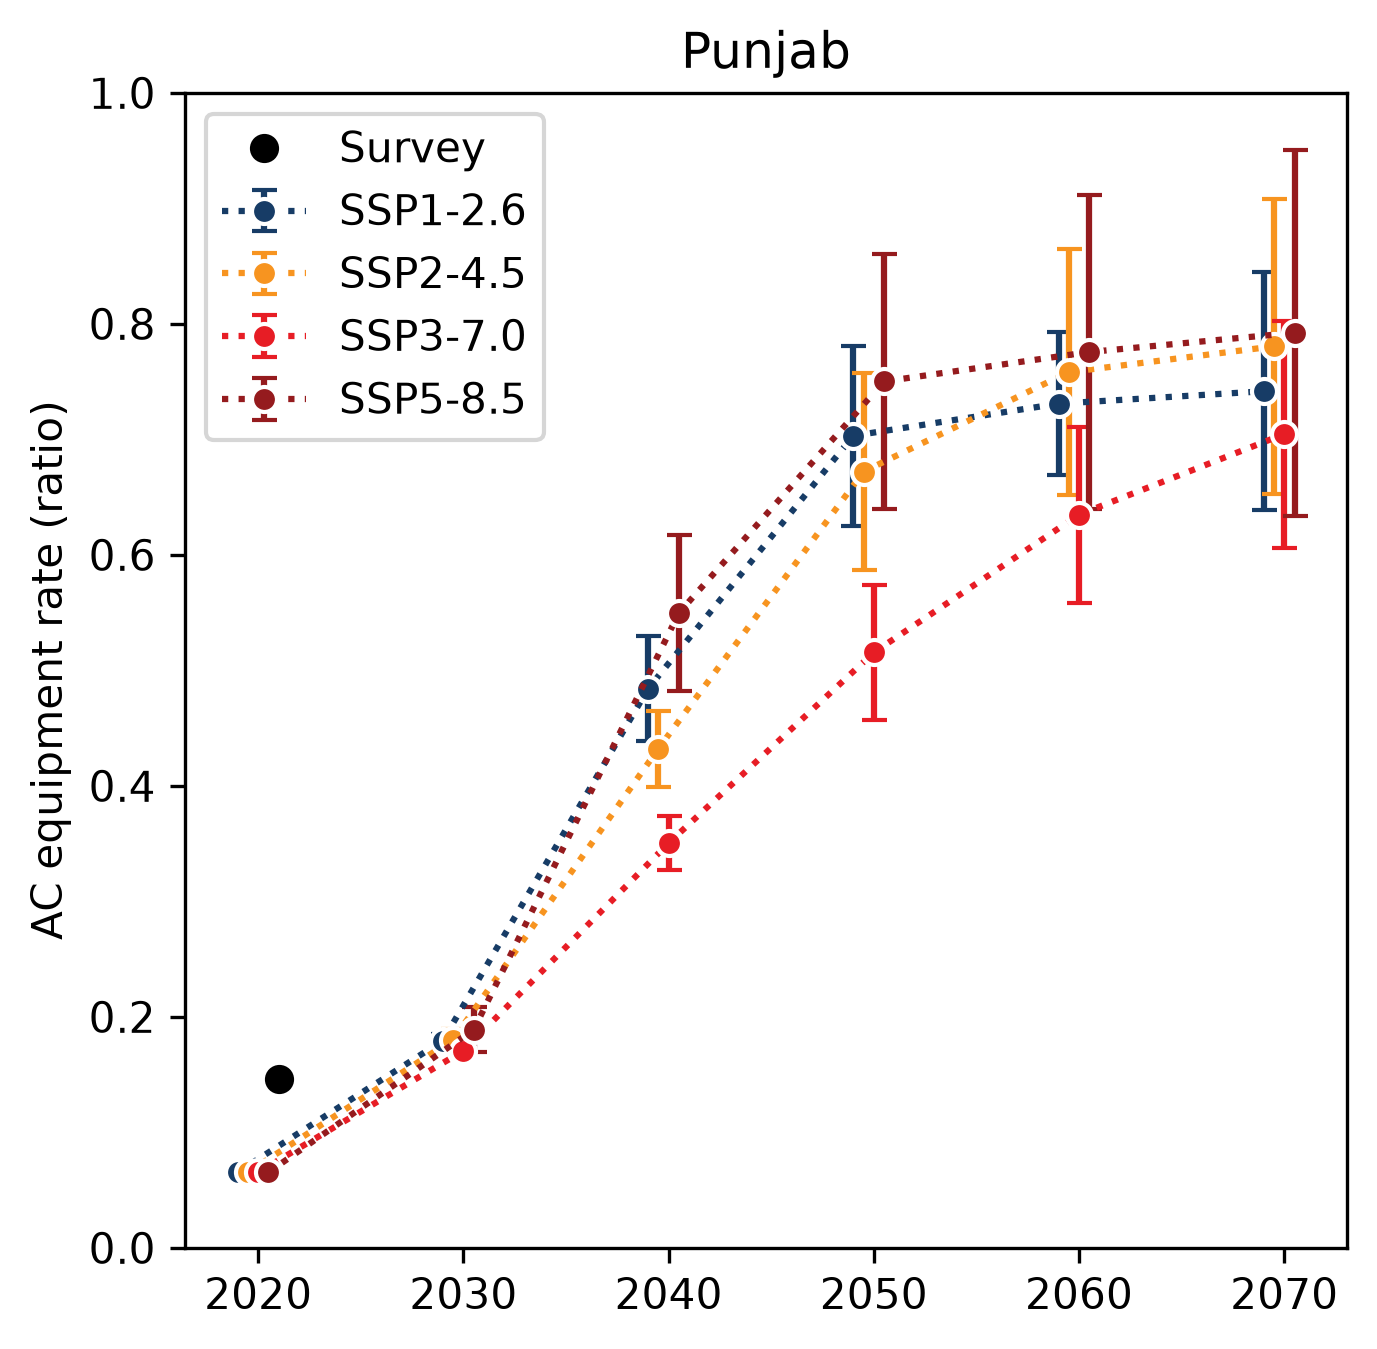
\includegraphics[height=0.25\textheight]{figures/projection_states/projection_ac_rate_Punjab.png}\hfill
   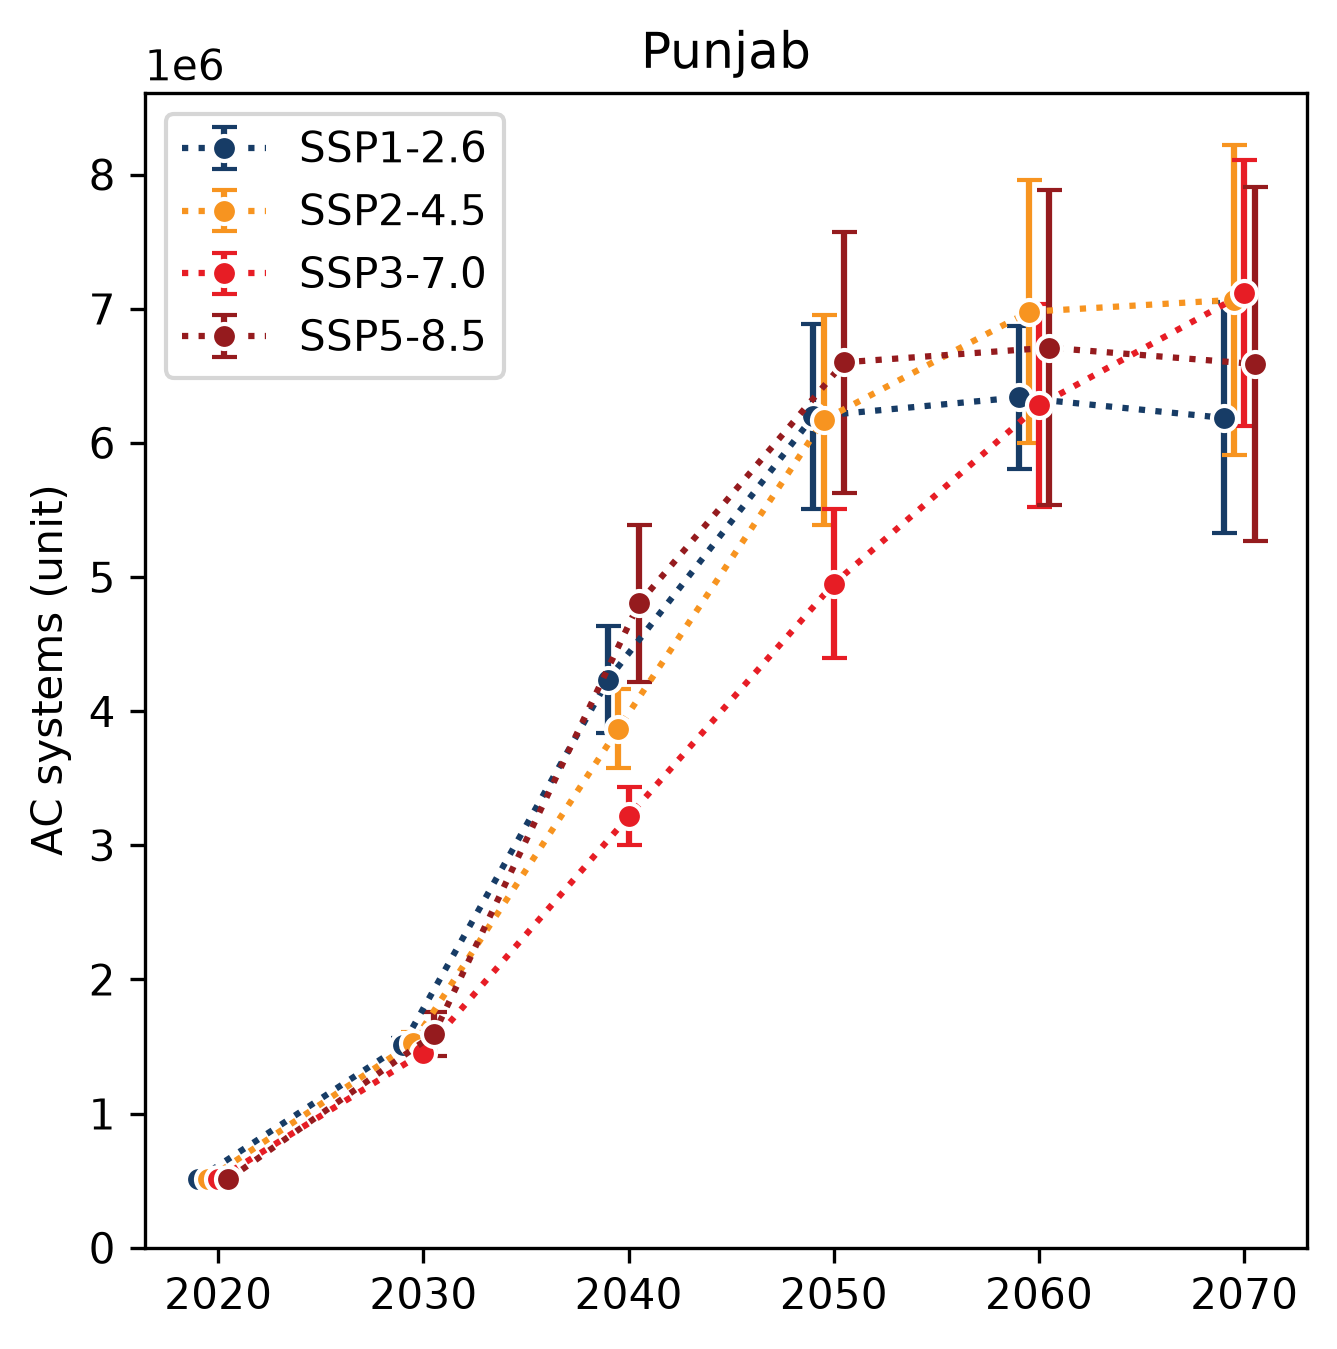
\includegraphics[height=0.25\textheight]{figures/projection_states/projection_ac_systems_Punjab.png}
   \caption{Projections des différentes variables pour Punjab}
\end{figure}

\clearpage

\subsubsection{Rajasthan}

\begin{figure}[ht]
   \centering
   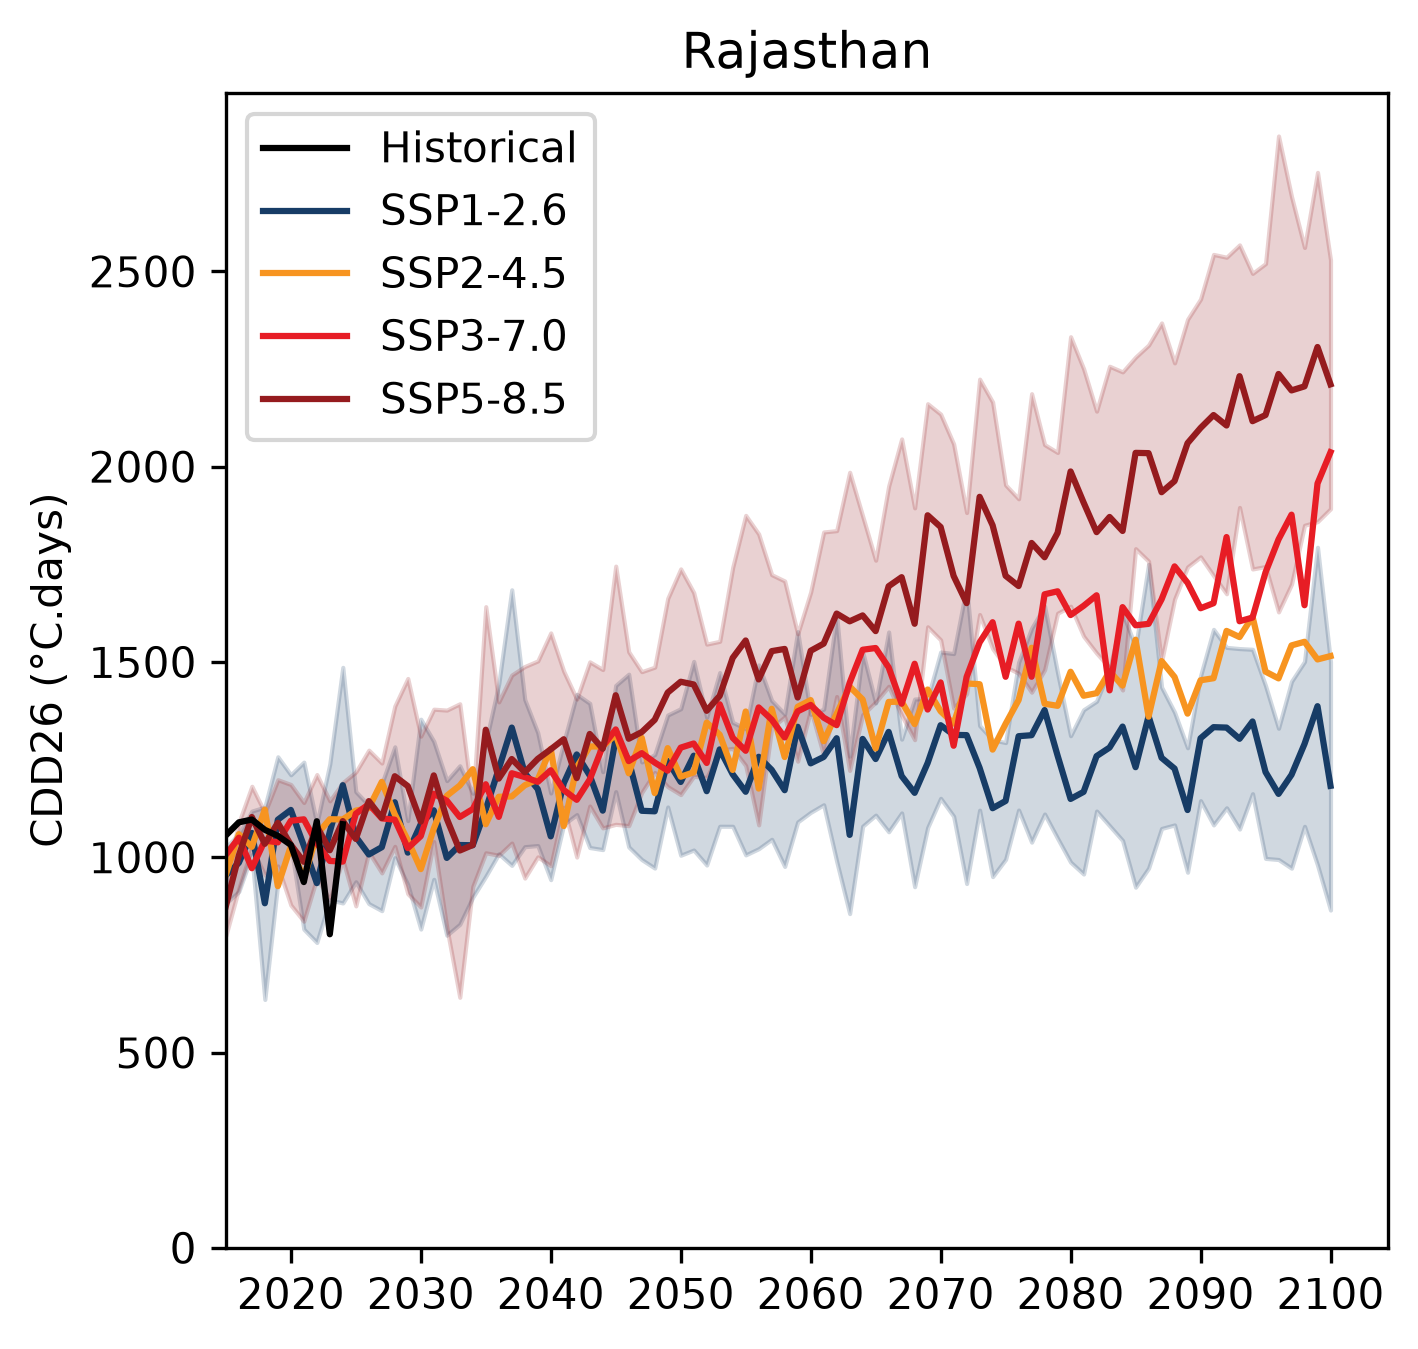
\includegraphics[height=0.25\textheight]{figures/projection_states/projection_cdd26_Rajasthan.png}\hfill
   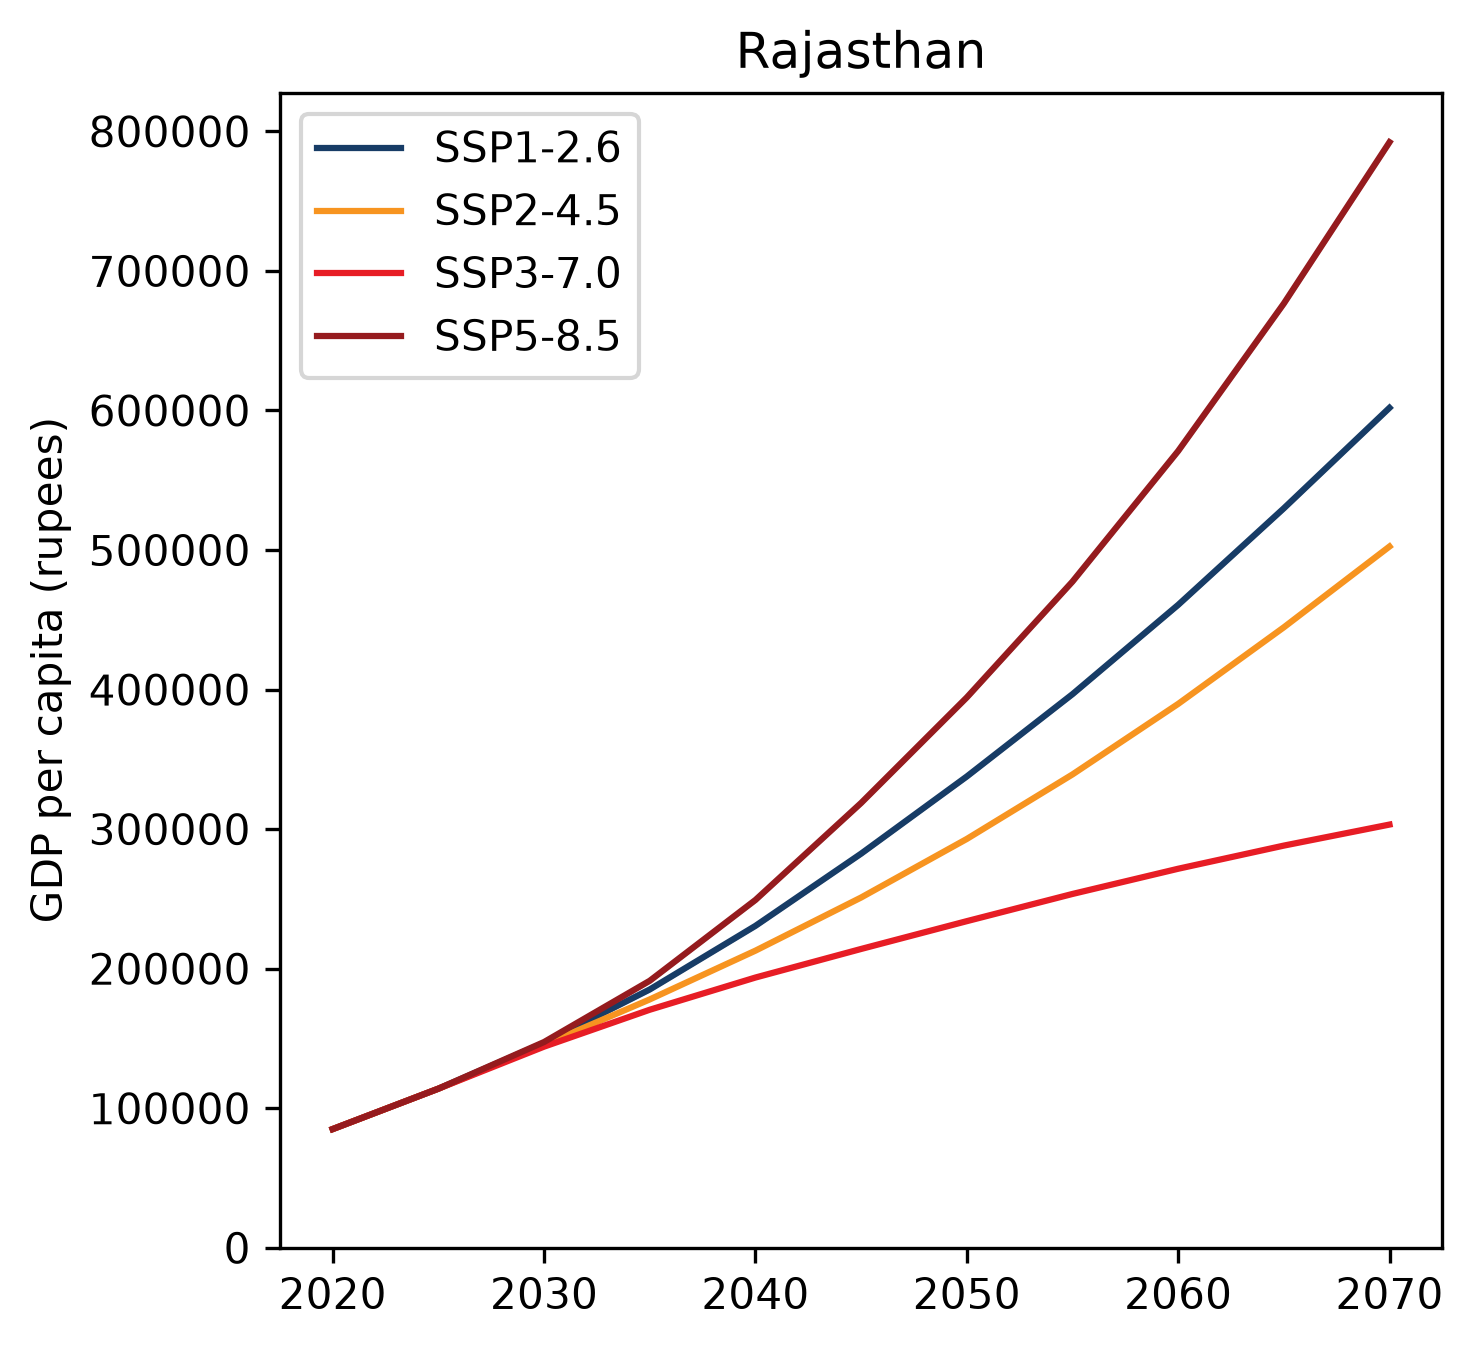
\includegraphics[height=0.25\textheight]{figures/projection_states/projection_gdp_per_capita_Rajasthan.png}\\
   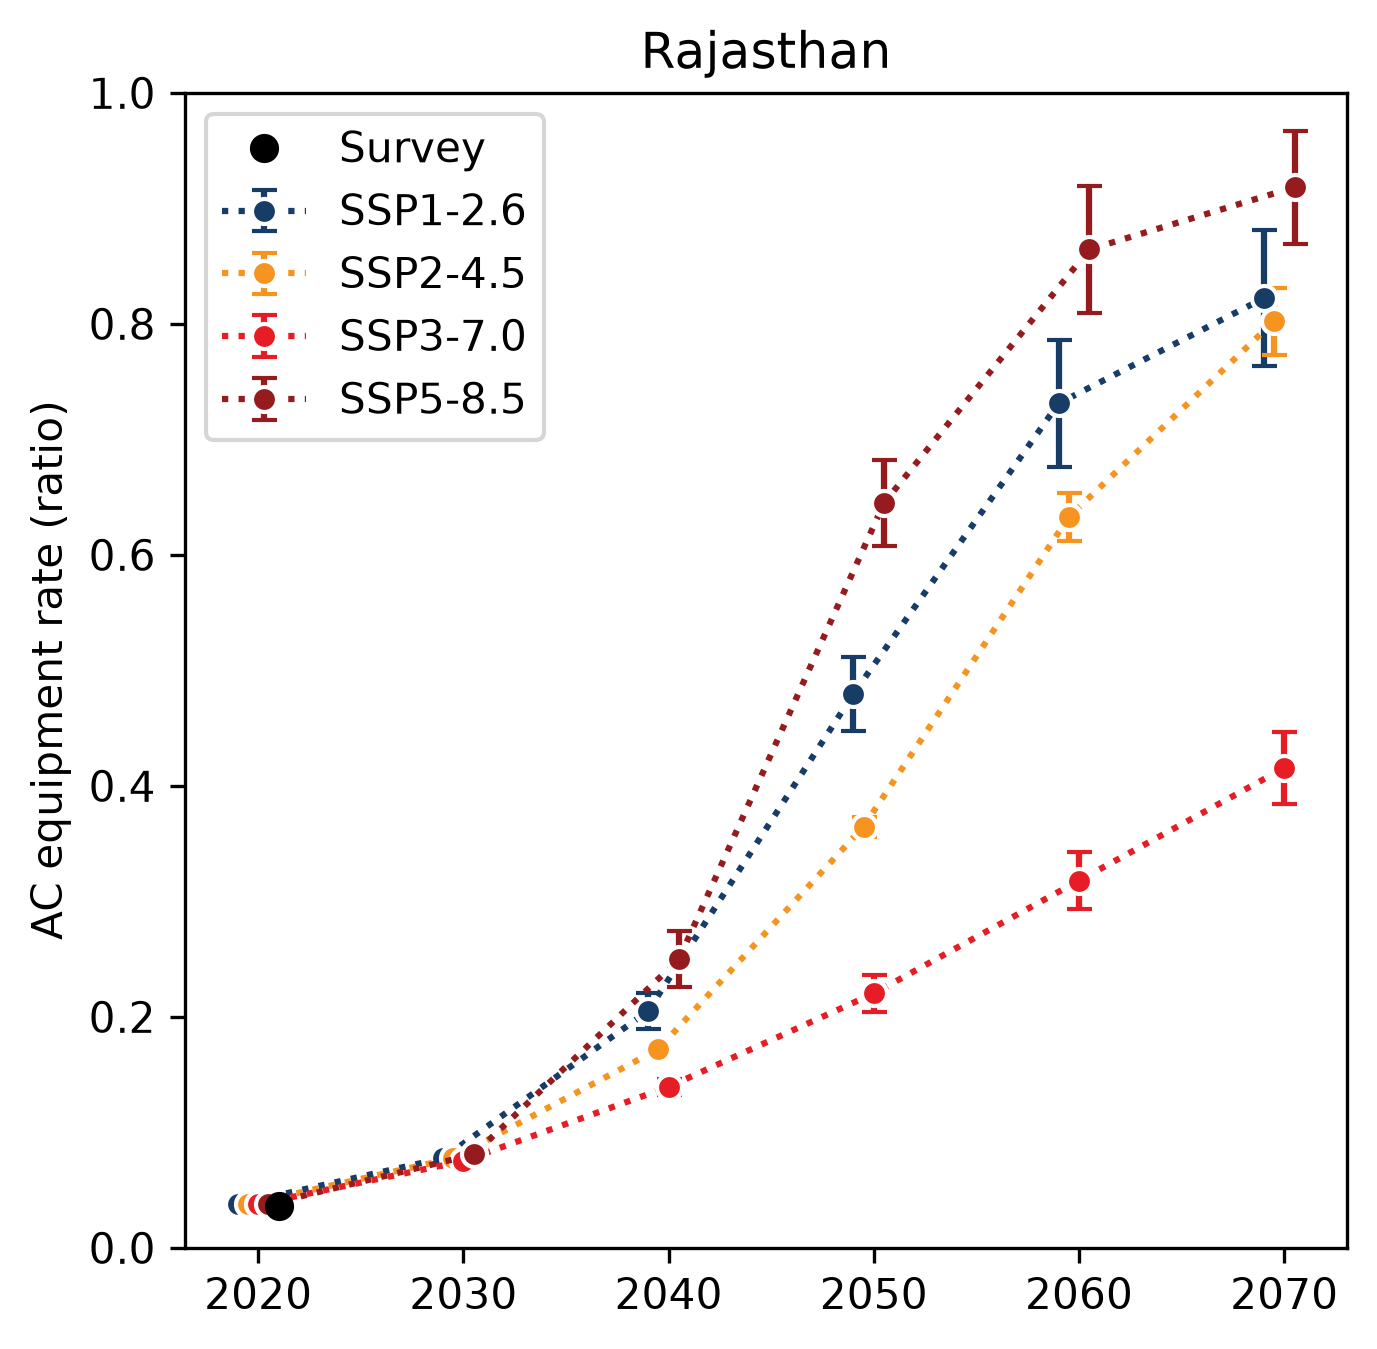
\includegraphics[height=0.25\textheight]{figures/projection_states/projection_ac_rate_Rajasthan.png}\hfill
   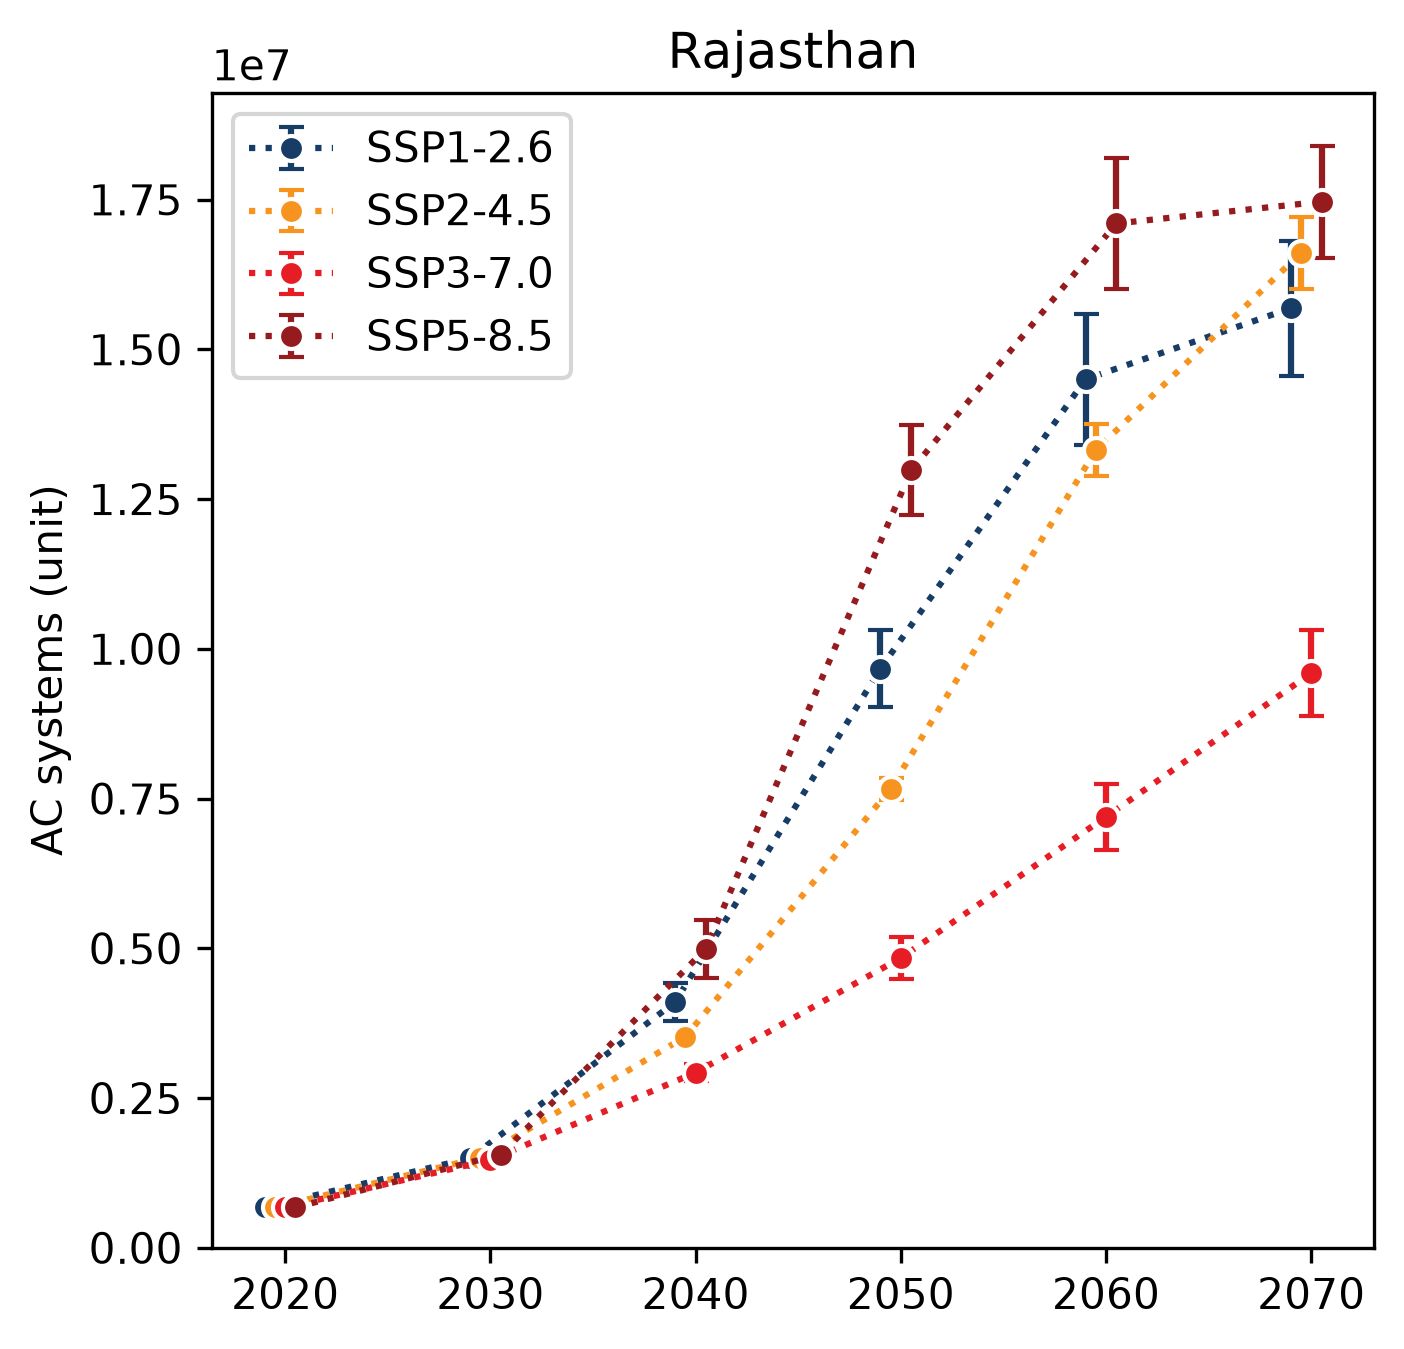
\includegraphics[height=0.25\textheight]{figures/projection_states/projection_ac_systems_Rajasthan.png}
   \caption{Projections des différentes variables pour Rajasthan}
\end{figure}

\clearpage

\subsubsection{Sikkim}

\begin{figure}[ht]
   \centering
   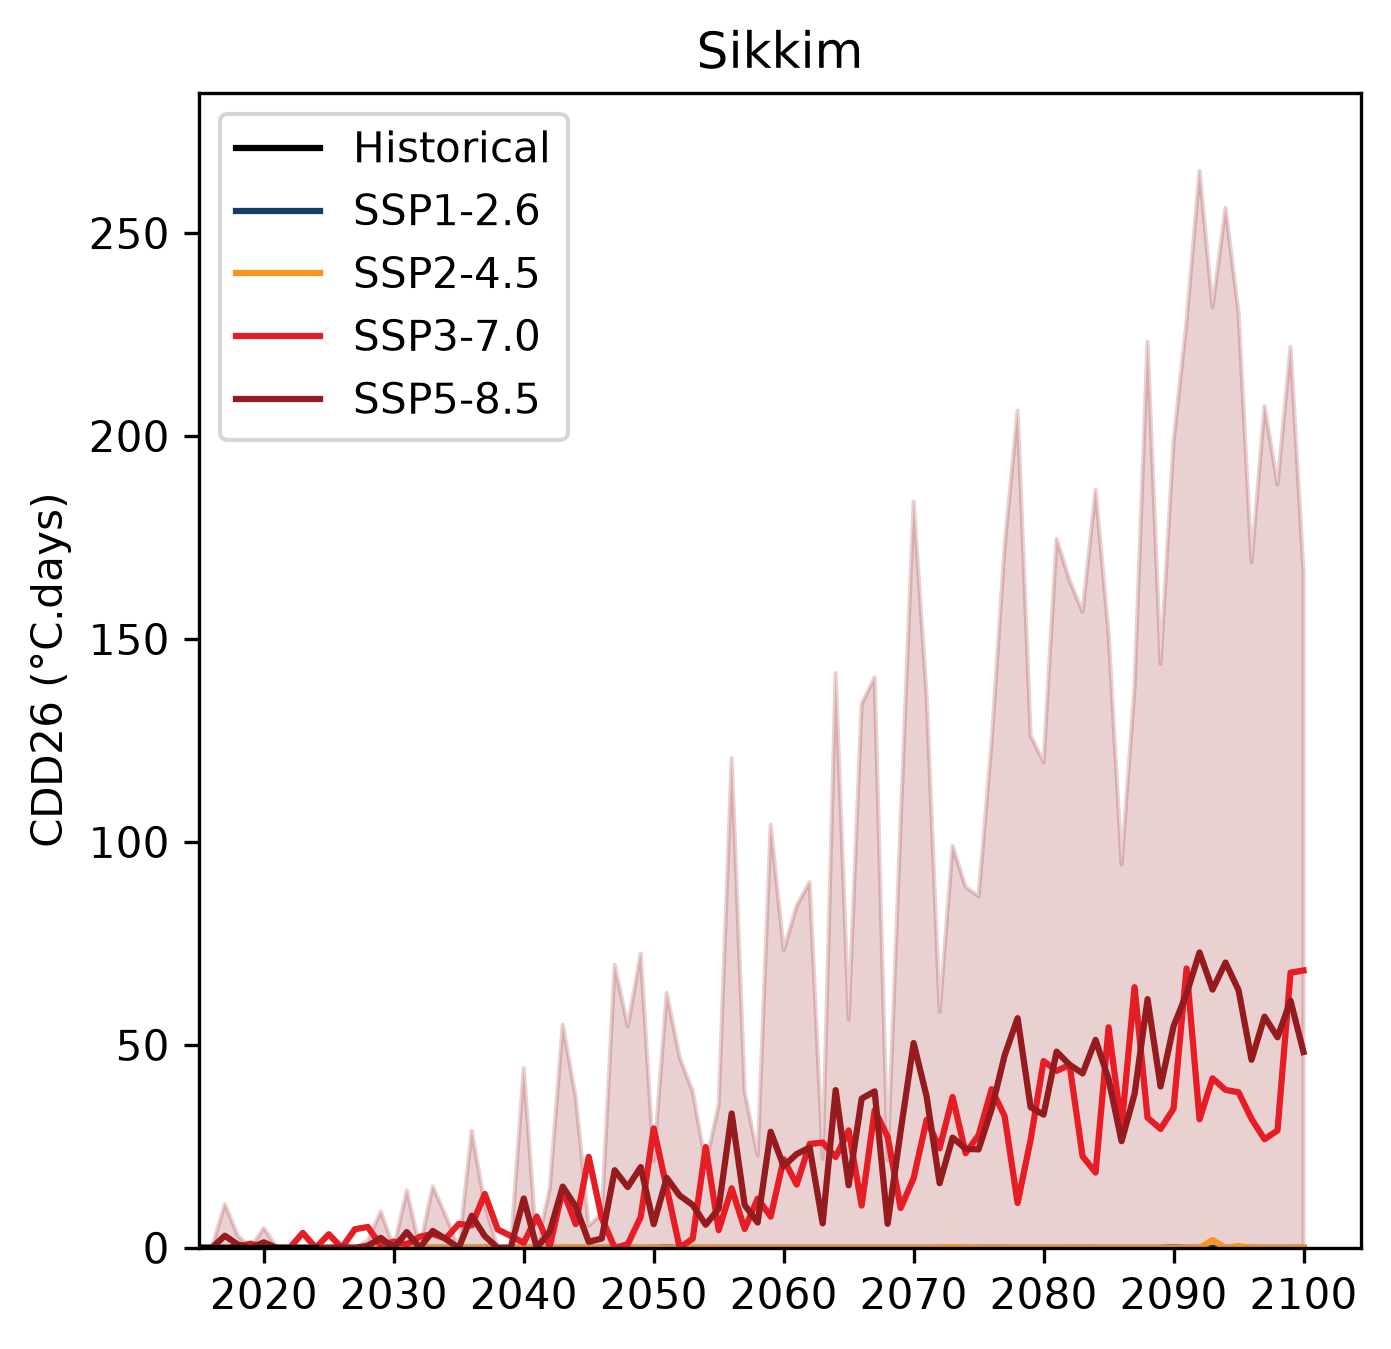
\includegraphics[height=0.25\textheight]{figures/projection_states/projection_cdd26_Sikkim.png}\hfill
   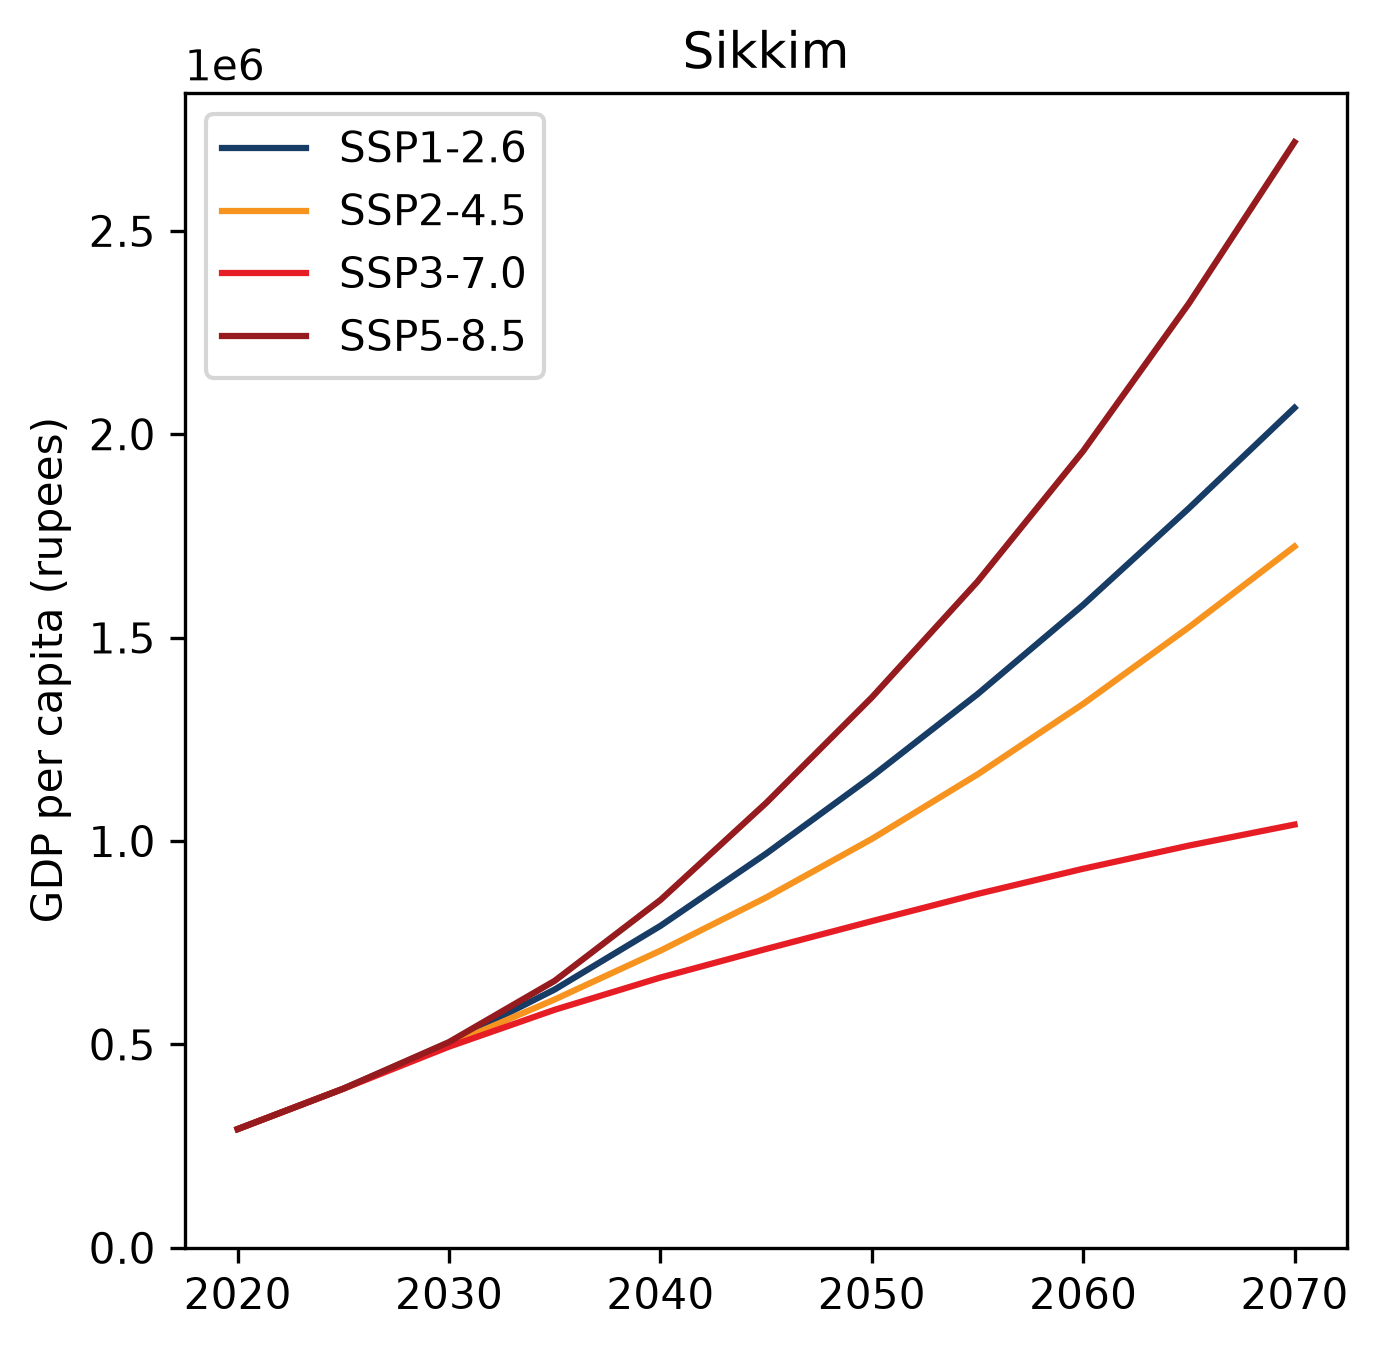
\includegraphics[height=0.25\textheight]{figures/projection_states/projection_gdp_per_capita_Sikkim.png}\\
   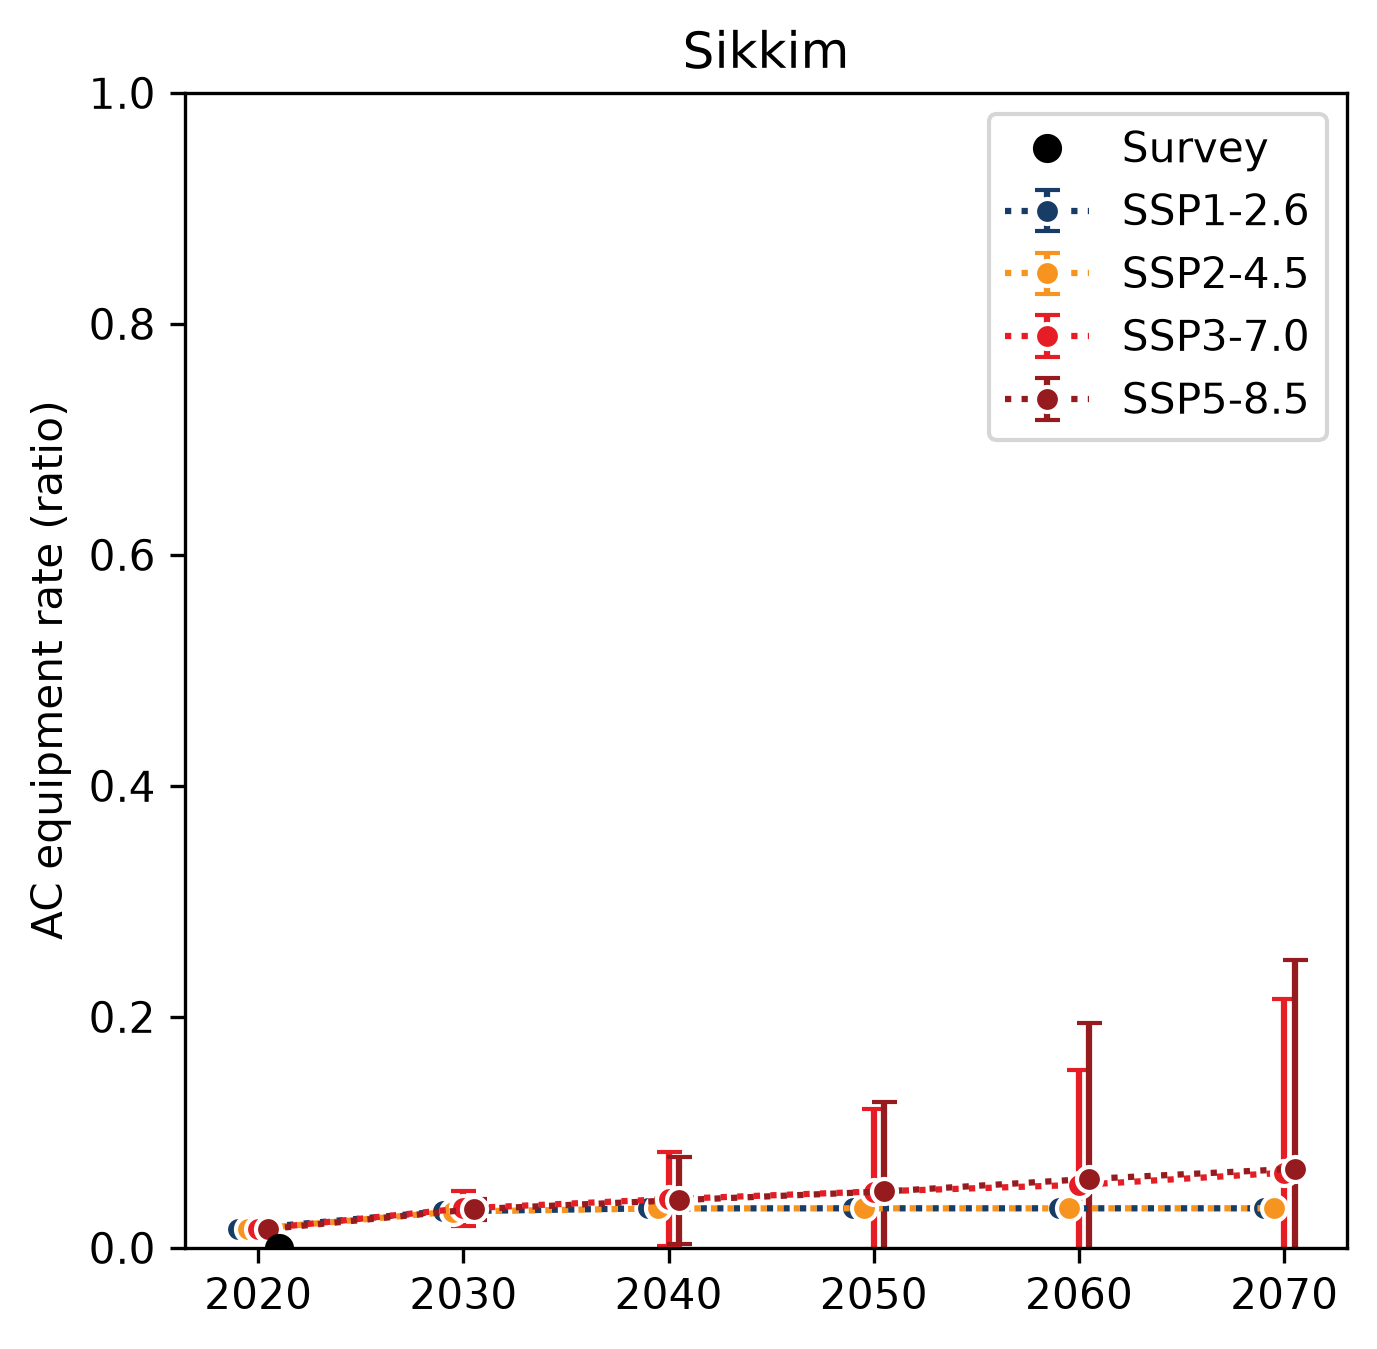
\includegraphics[height=0.25\textheight]{figures/projection_states/projection_ac_rate_Sikkim.png}\hfill
   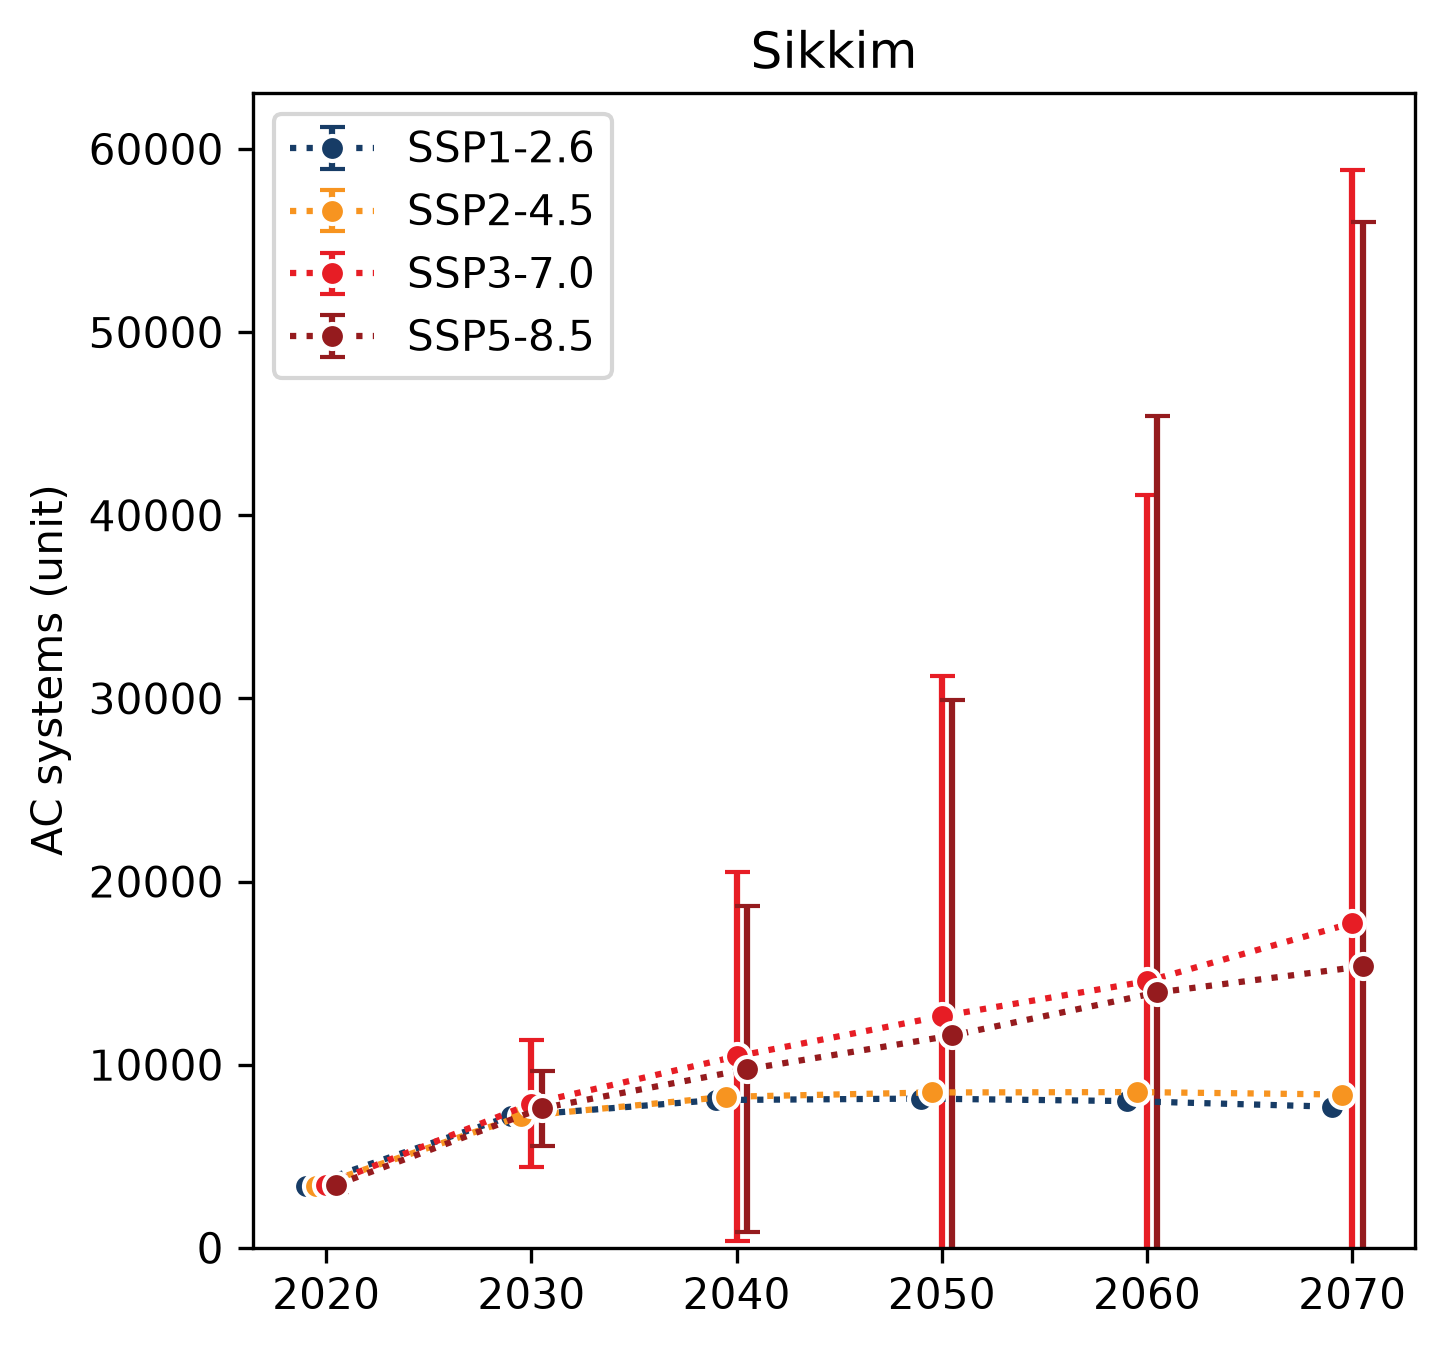
\includegraphics[height=0.25\textheight]{figures/projection_states/projection_ac_systems_Sikkim.png}
   \caption{Projections des différentes variables pour Sikkim}
\end{figure}

\clearpage

\subsubsection{Tamil Nadu}

\begin{figure}[ht]
   \centering
   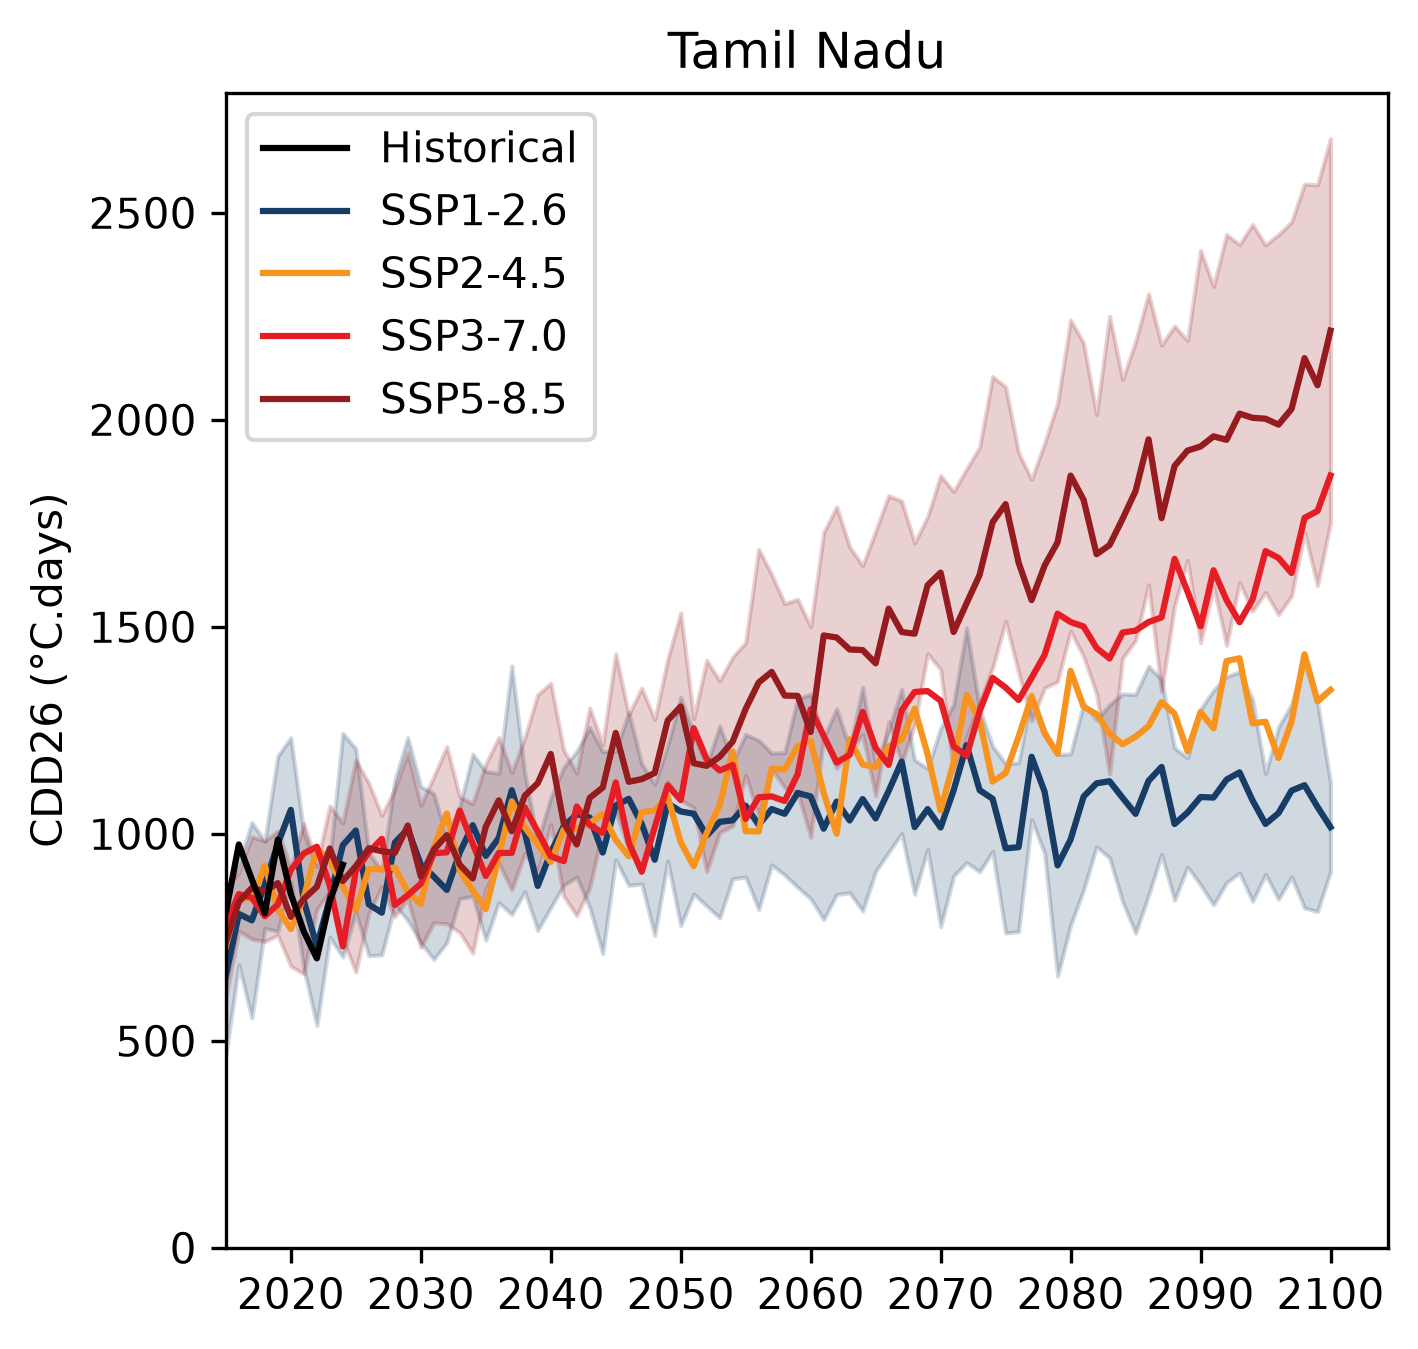
\includegraphics[height=0.25\textheight]{figures/projection_states/projection_cdd26_Tamil Nadu.png}\hfill
   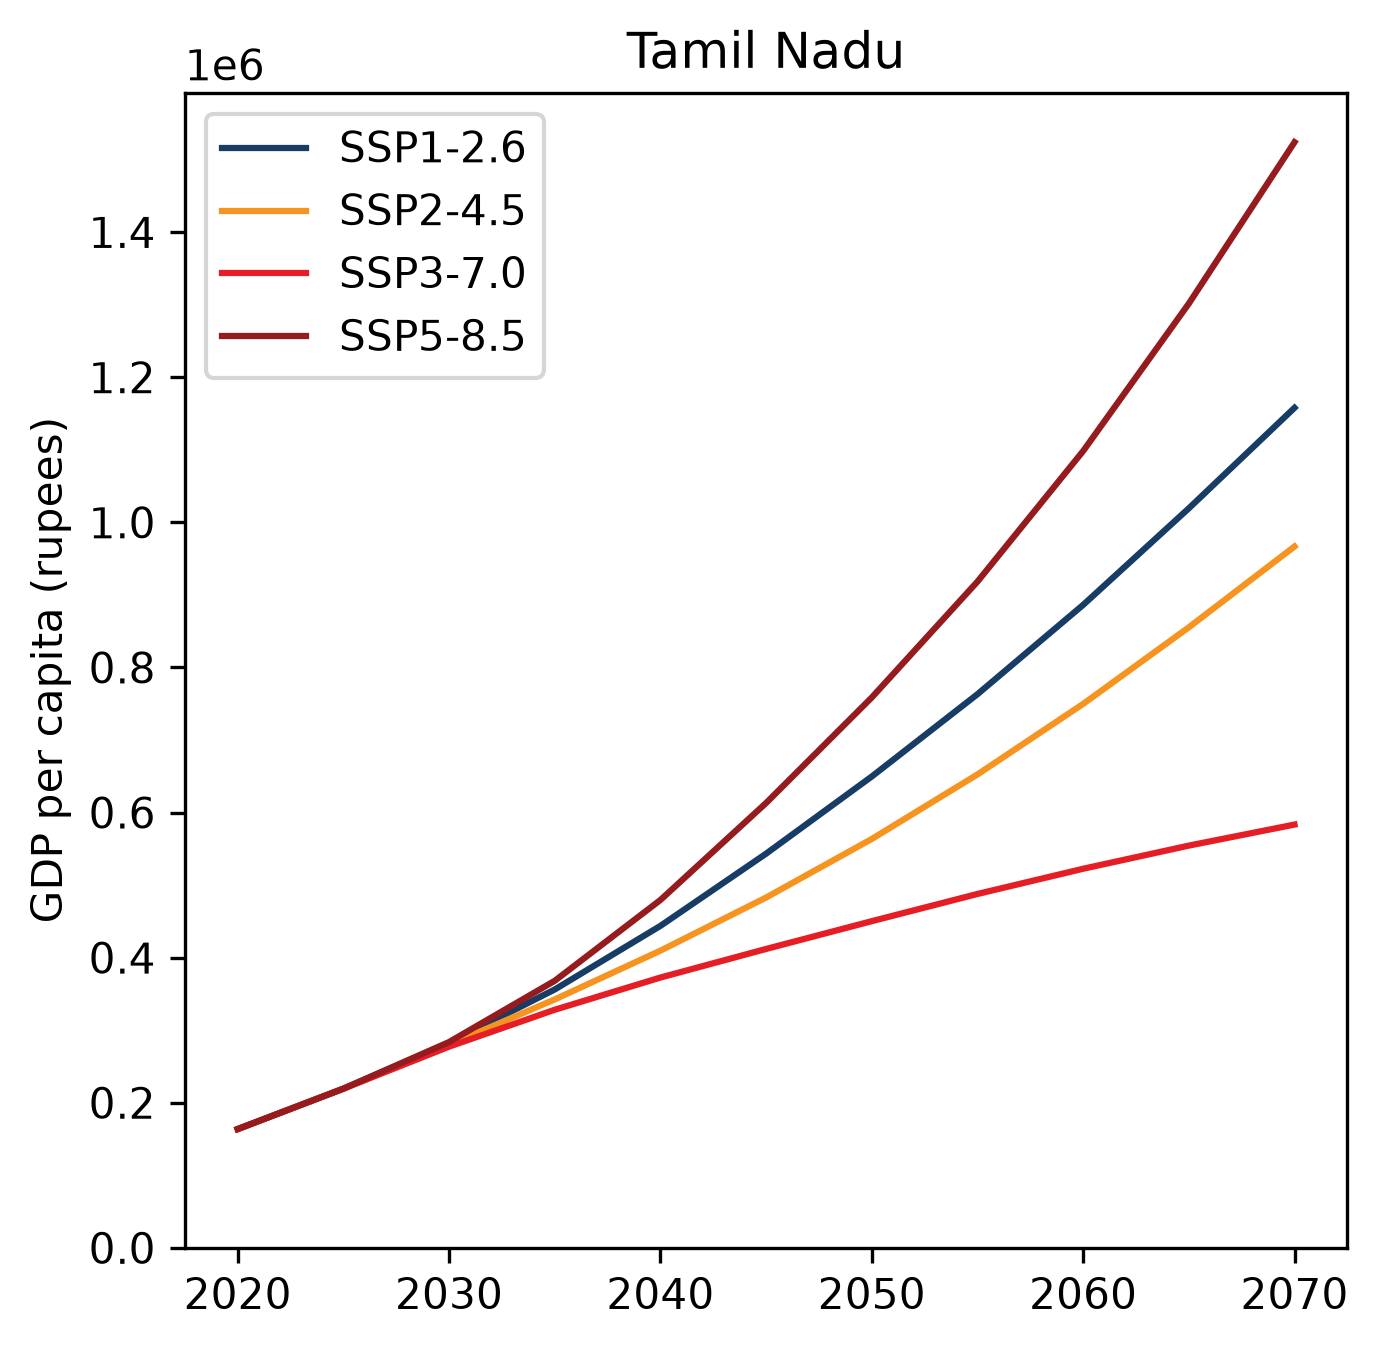
\includegraphics[height=0.25\textheight]{figures/projection_states/projection_gdp_per_capita_Tamil Nadu.png}\\
   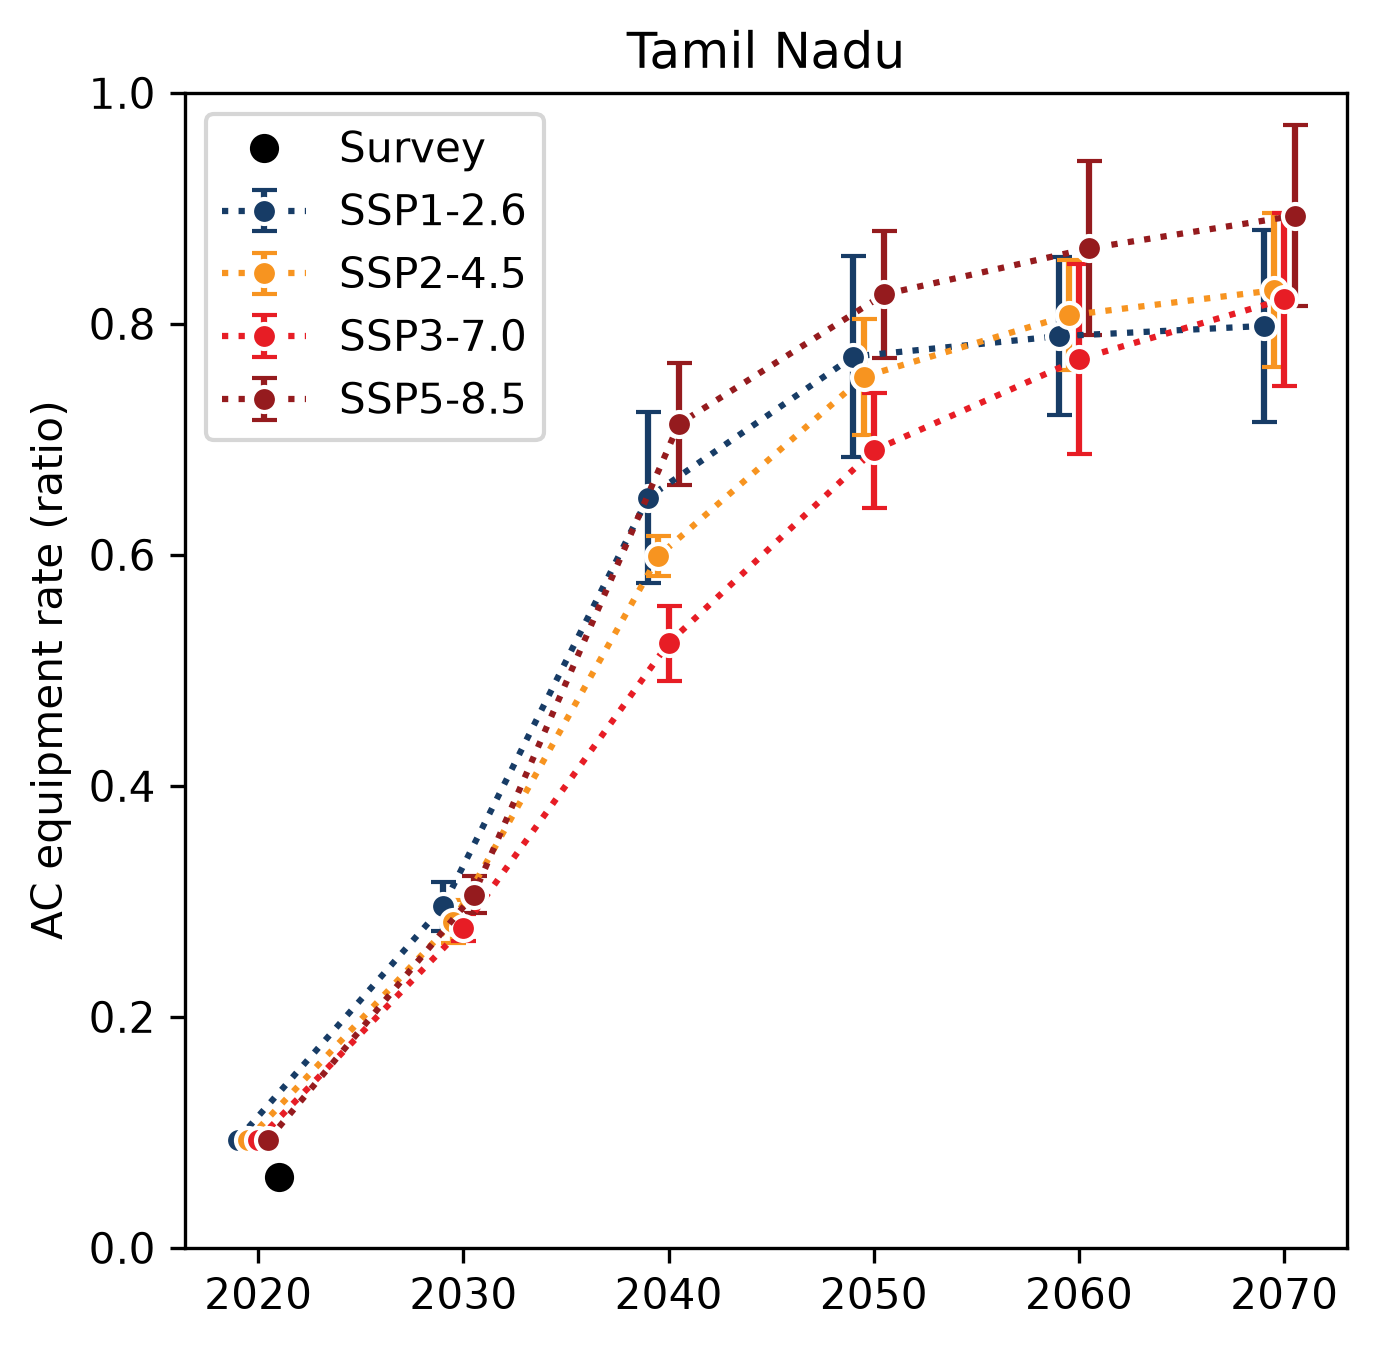
\includegraphics[height=0.25\textheight]{figures/projection_states/projection_ac_rate_Tamil Nadu.png}\hfill
   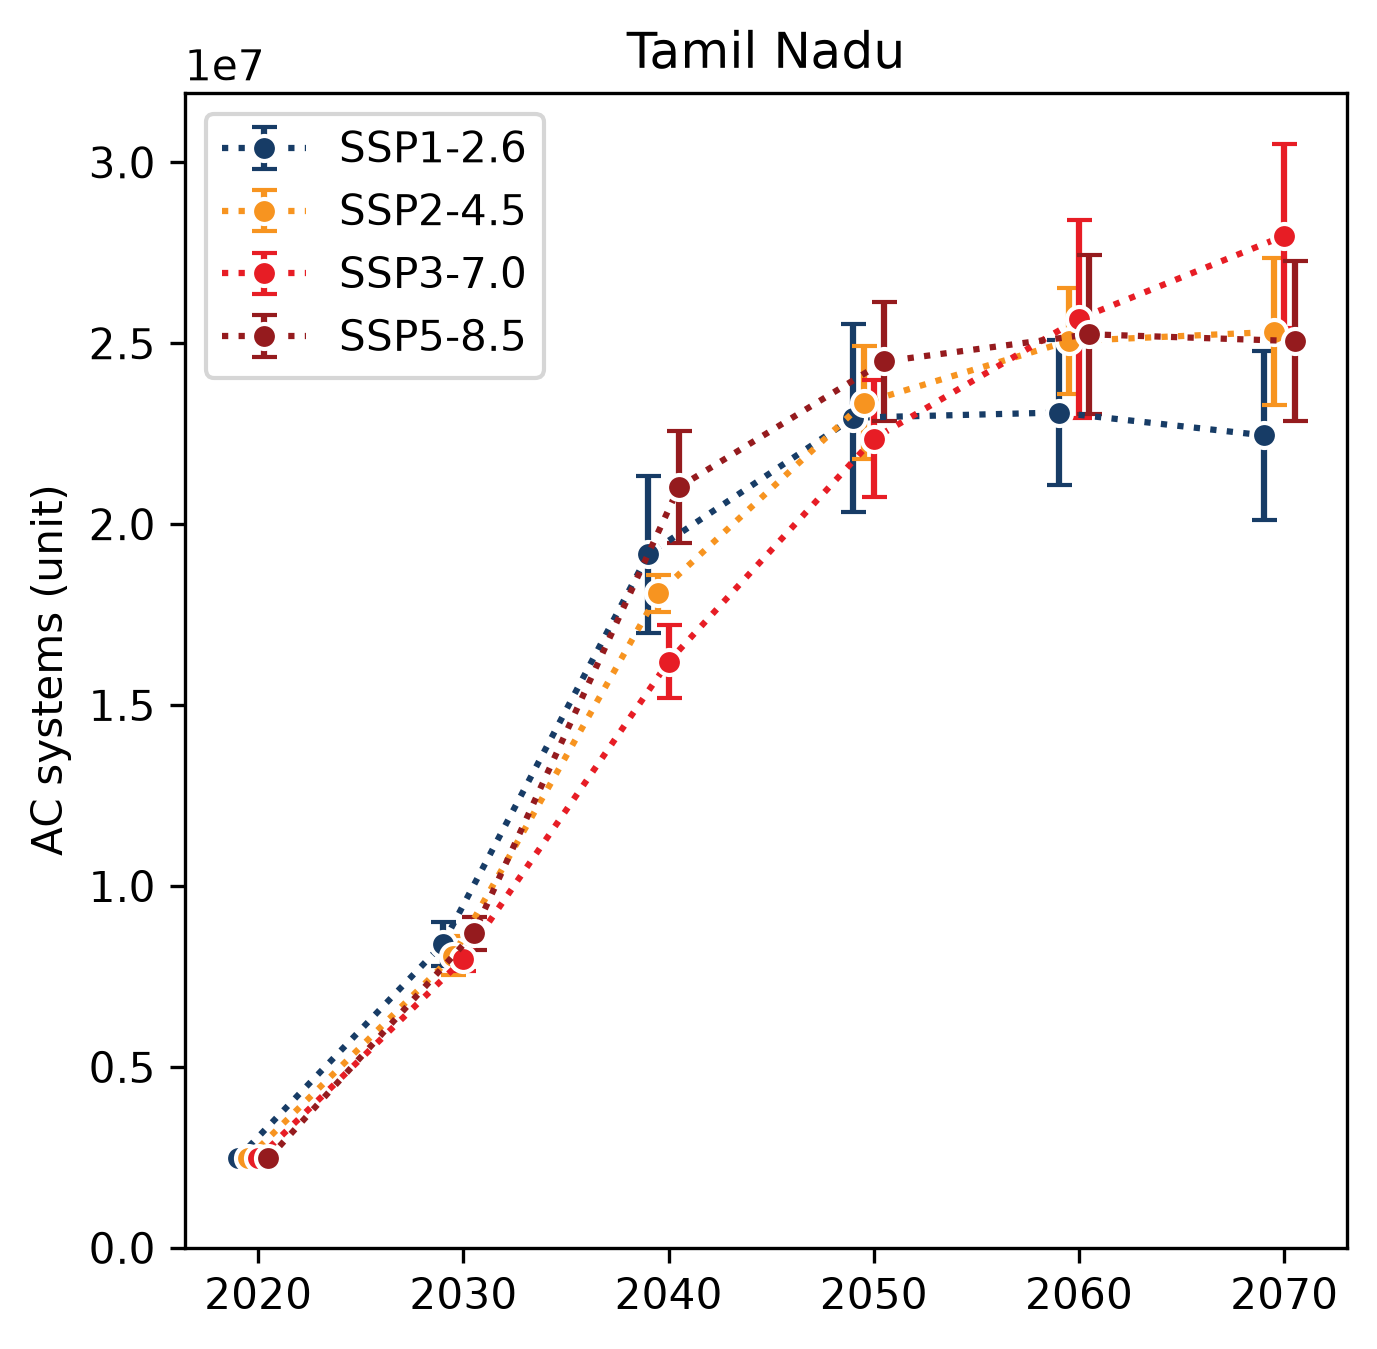
\includegraphics[height=0.25\textheight]{figures/projection_states/projection_ac_systems_Tamil Nadu.png}
   \caption{Projections des différentes variables pour Tamil Nadu}
\end{figure}

\clearpage

\subsubsection{Telangana}

\begin{figure}[ht]
   \centering
   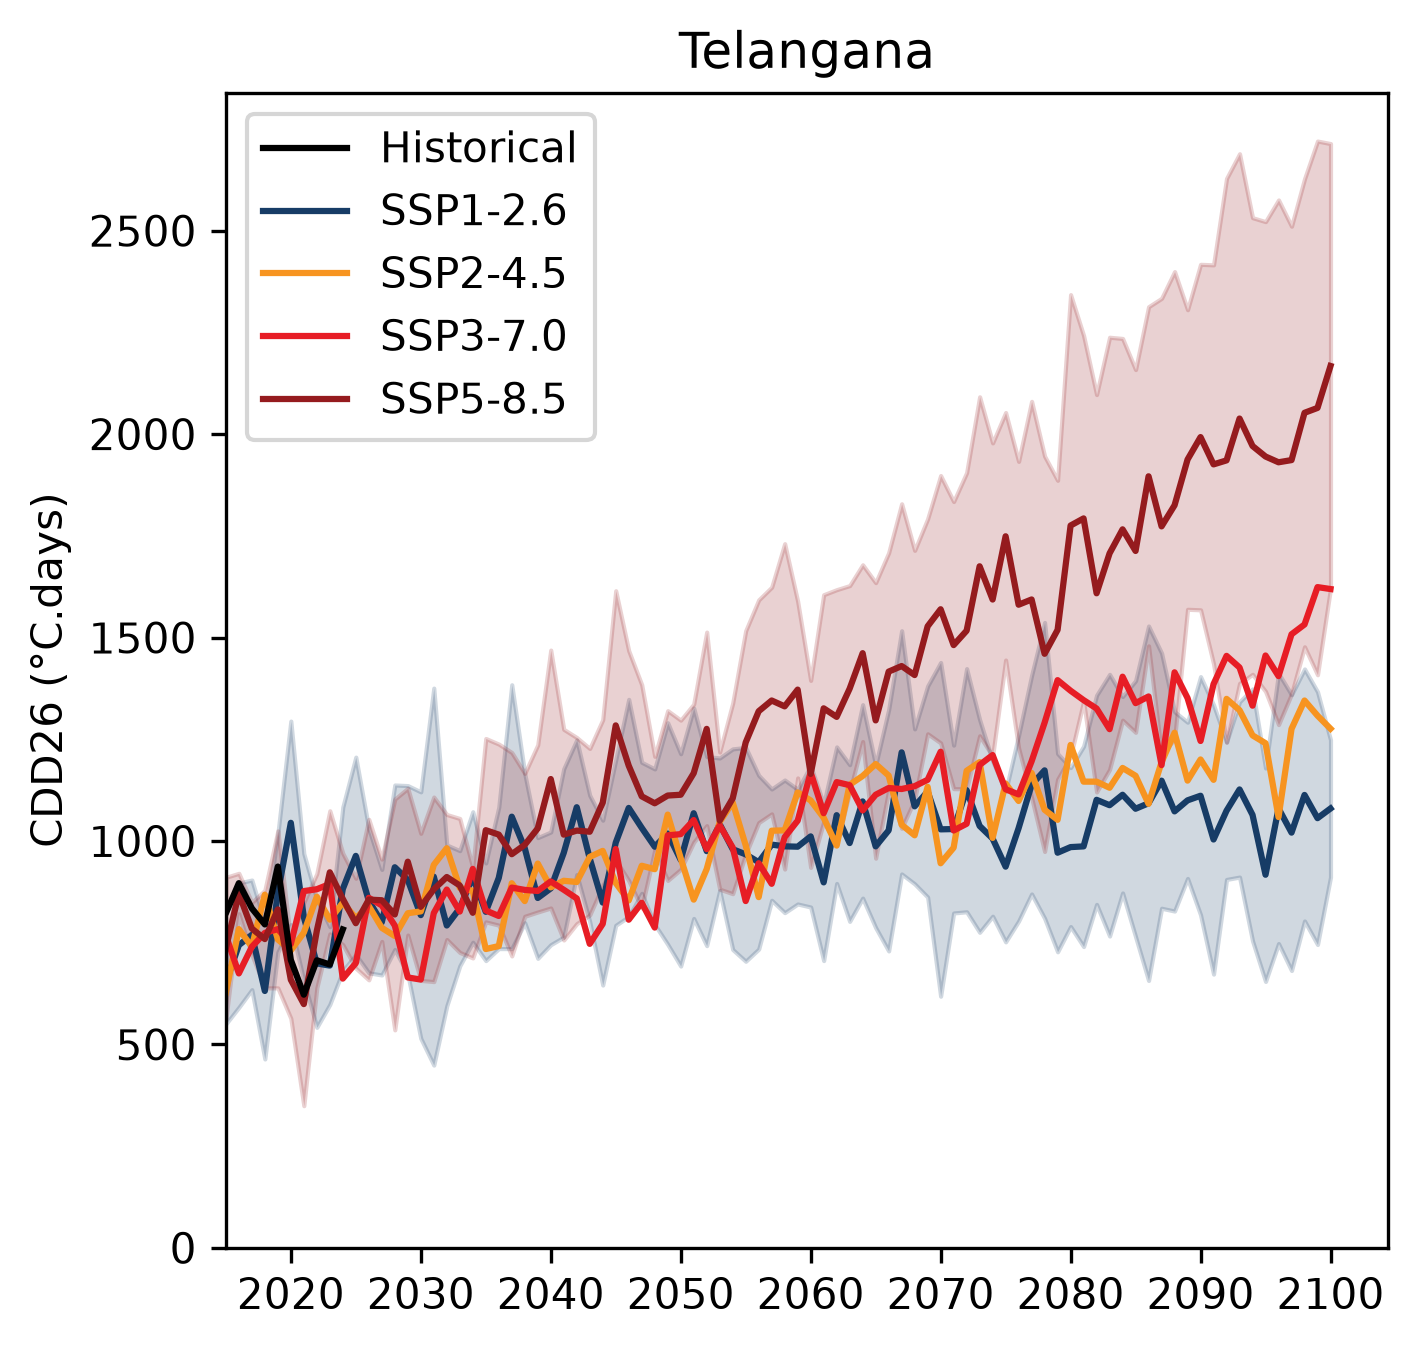
\includegraphics[height=0.25\textheight]{figures/projection_states/projection_cdd26_Telangana.png}\hfill
   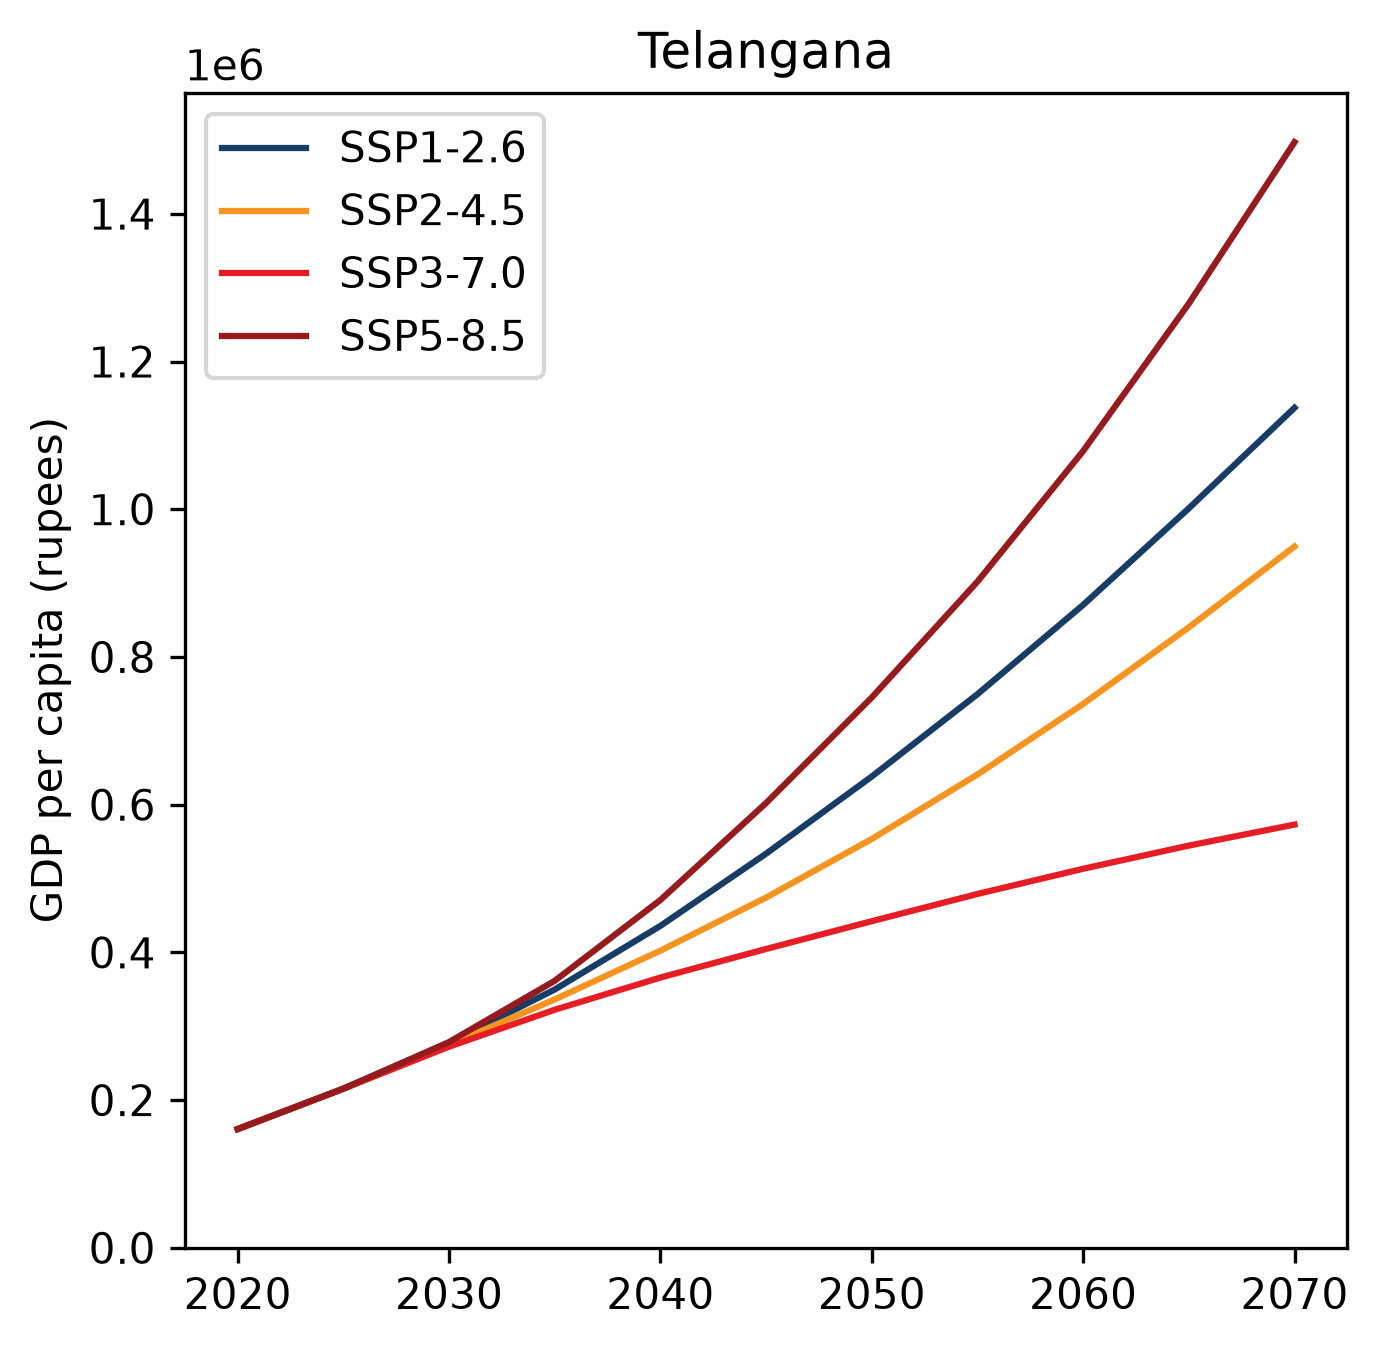
\includegraphics[height=0.25\textheight]{figures/projection_states/projection_gdp_per_capita_Telangana.png}\\
   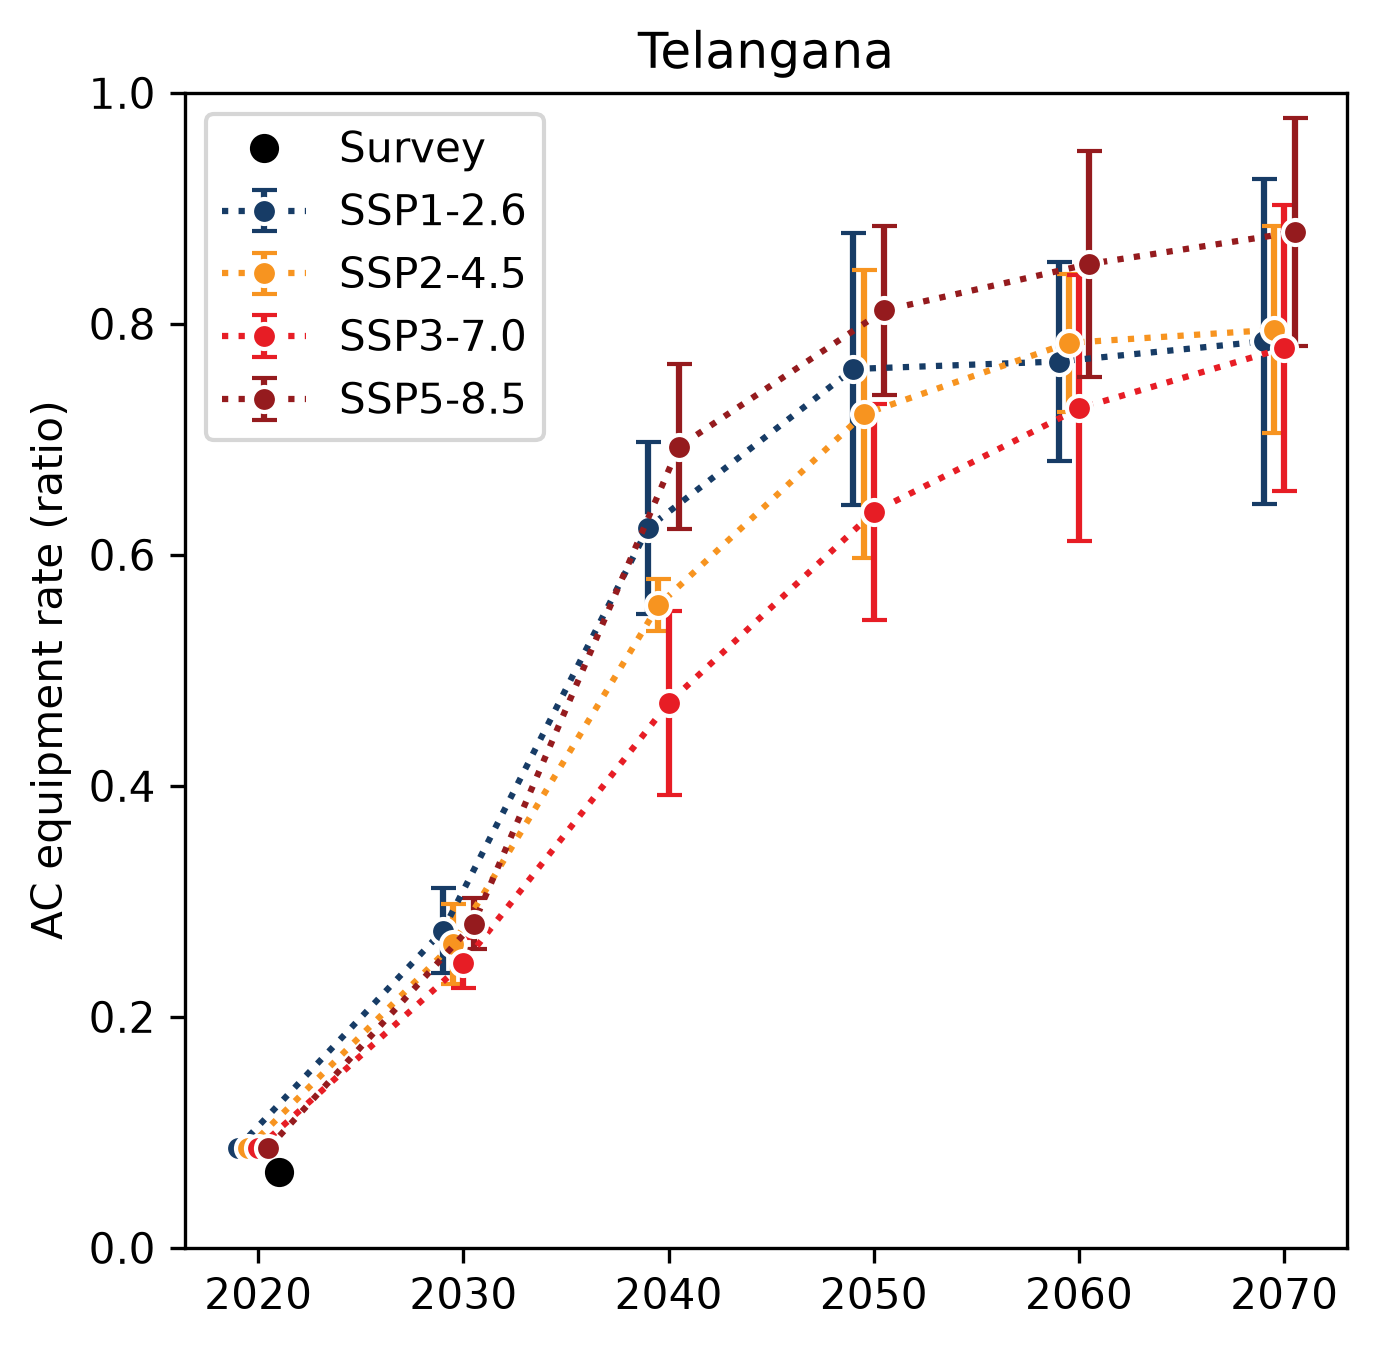
\includegraphics[height=0.25\textheight]{figures/projection_states/projection_ac_rate_Telangana.png}\hfill
   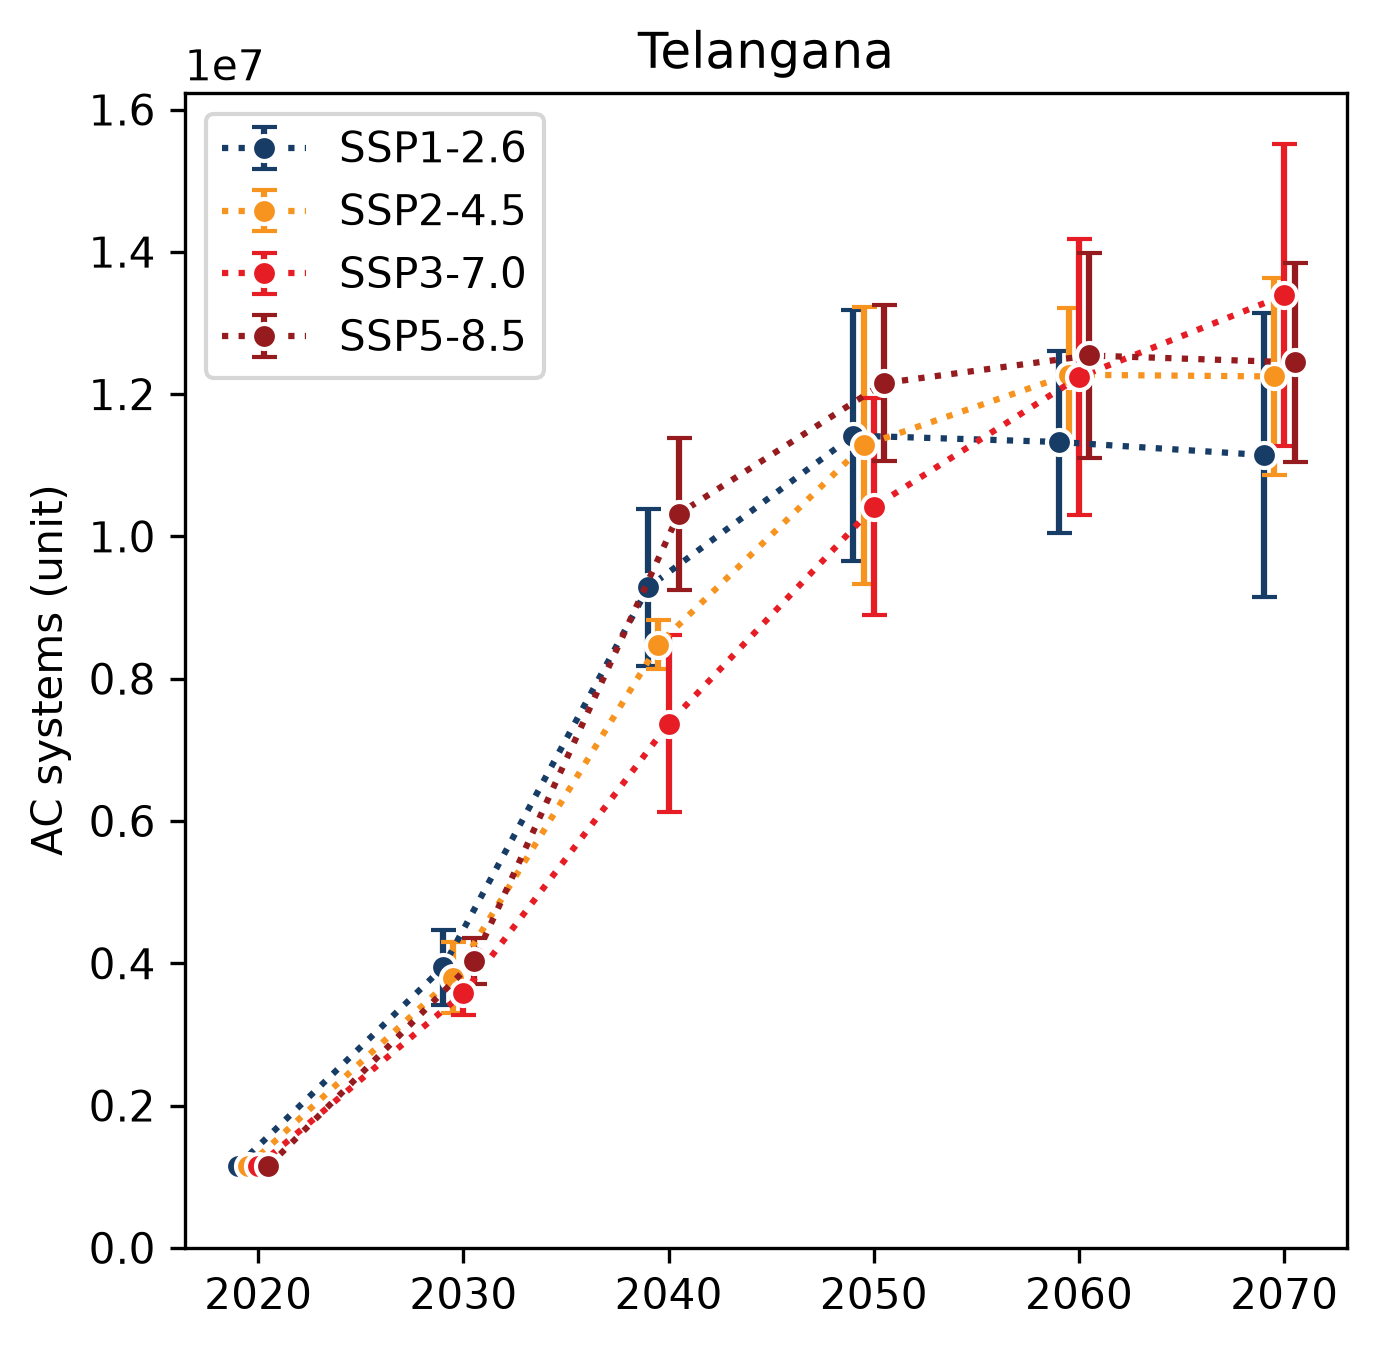
\includegraphics[height=0.25\textheight]{figures/projection_states/projection_ac_systems_Telangana.png}
   \caption{Projections des différentes variables pour Telangana}
\end{figure}

\clearpage

\subsubsection{Tripura}

\begin{figure}[ht]
   \centering
   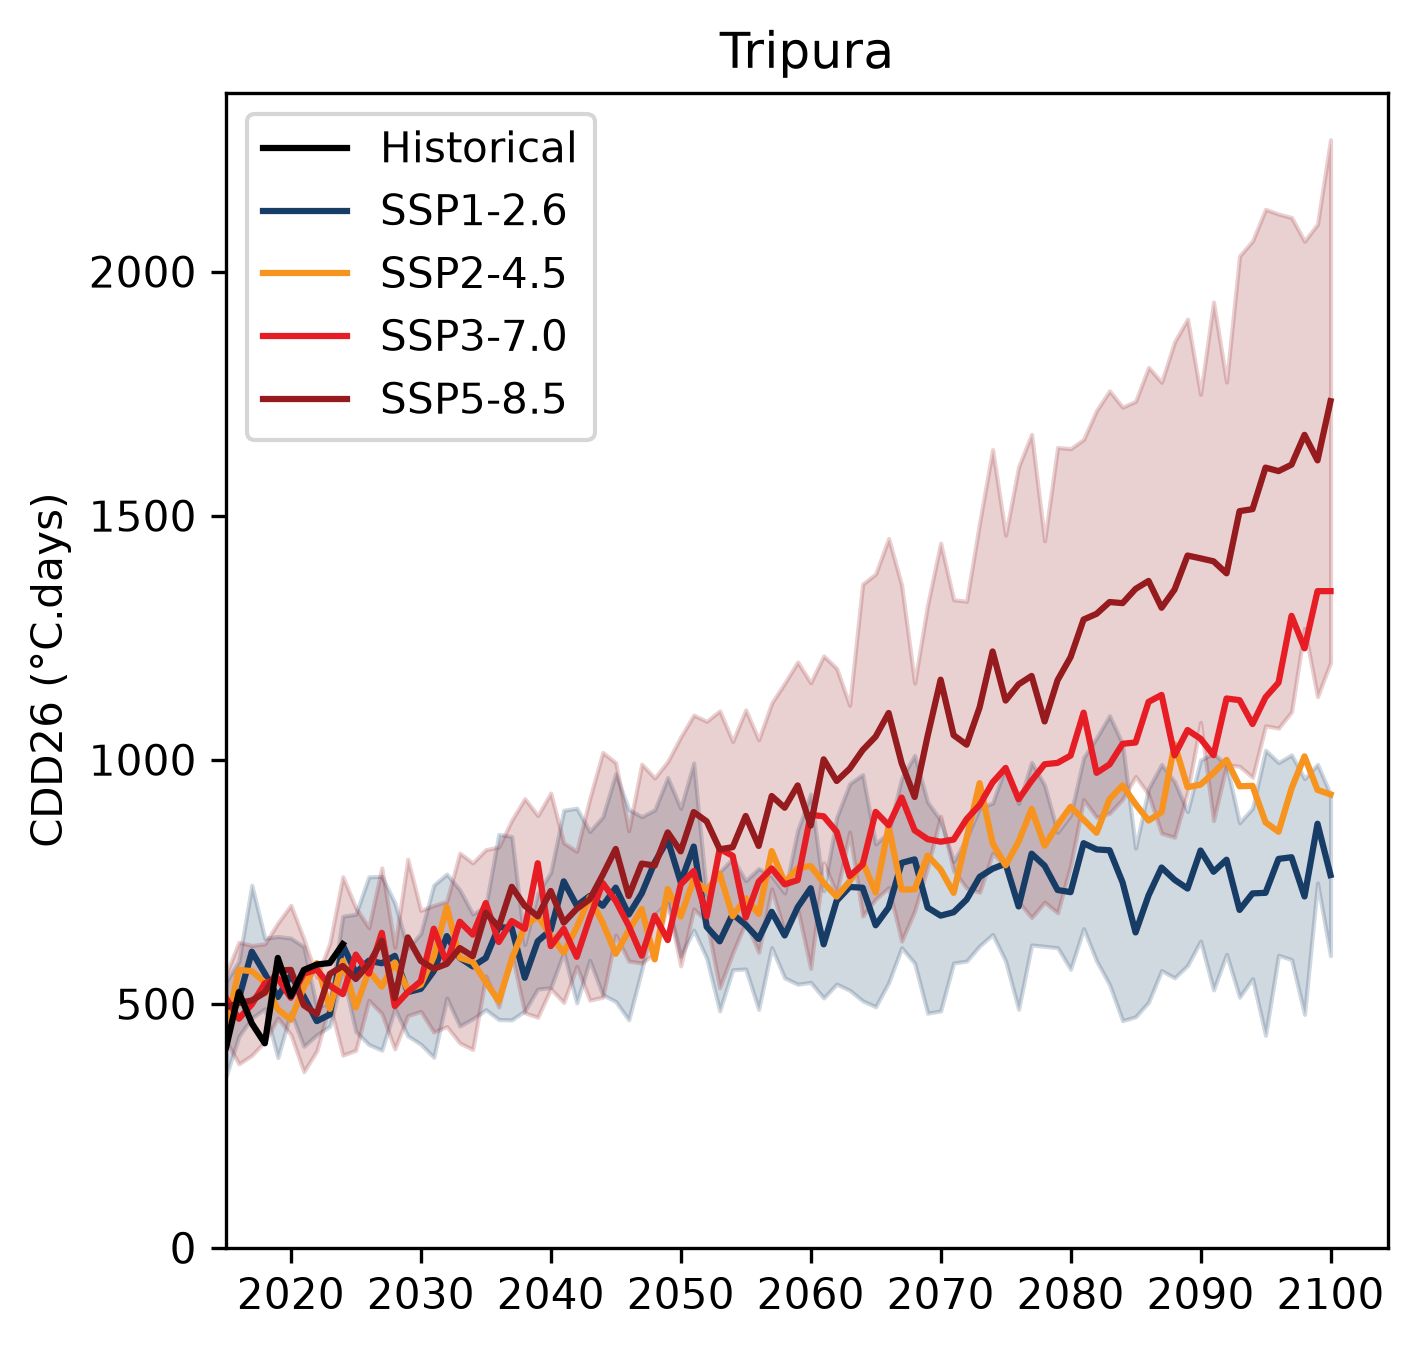
\includegraphics[height=0.25\textheight]{figures/projection_states/projection_cdd26_Tripura.png}\hfill
   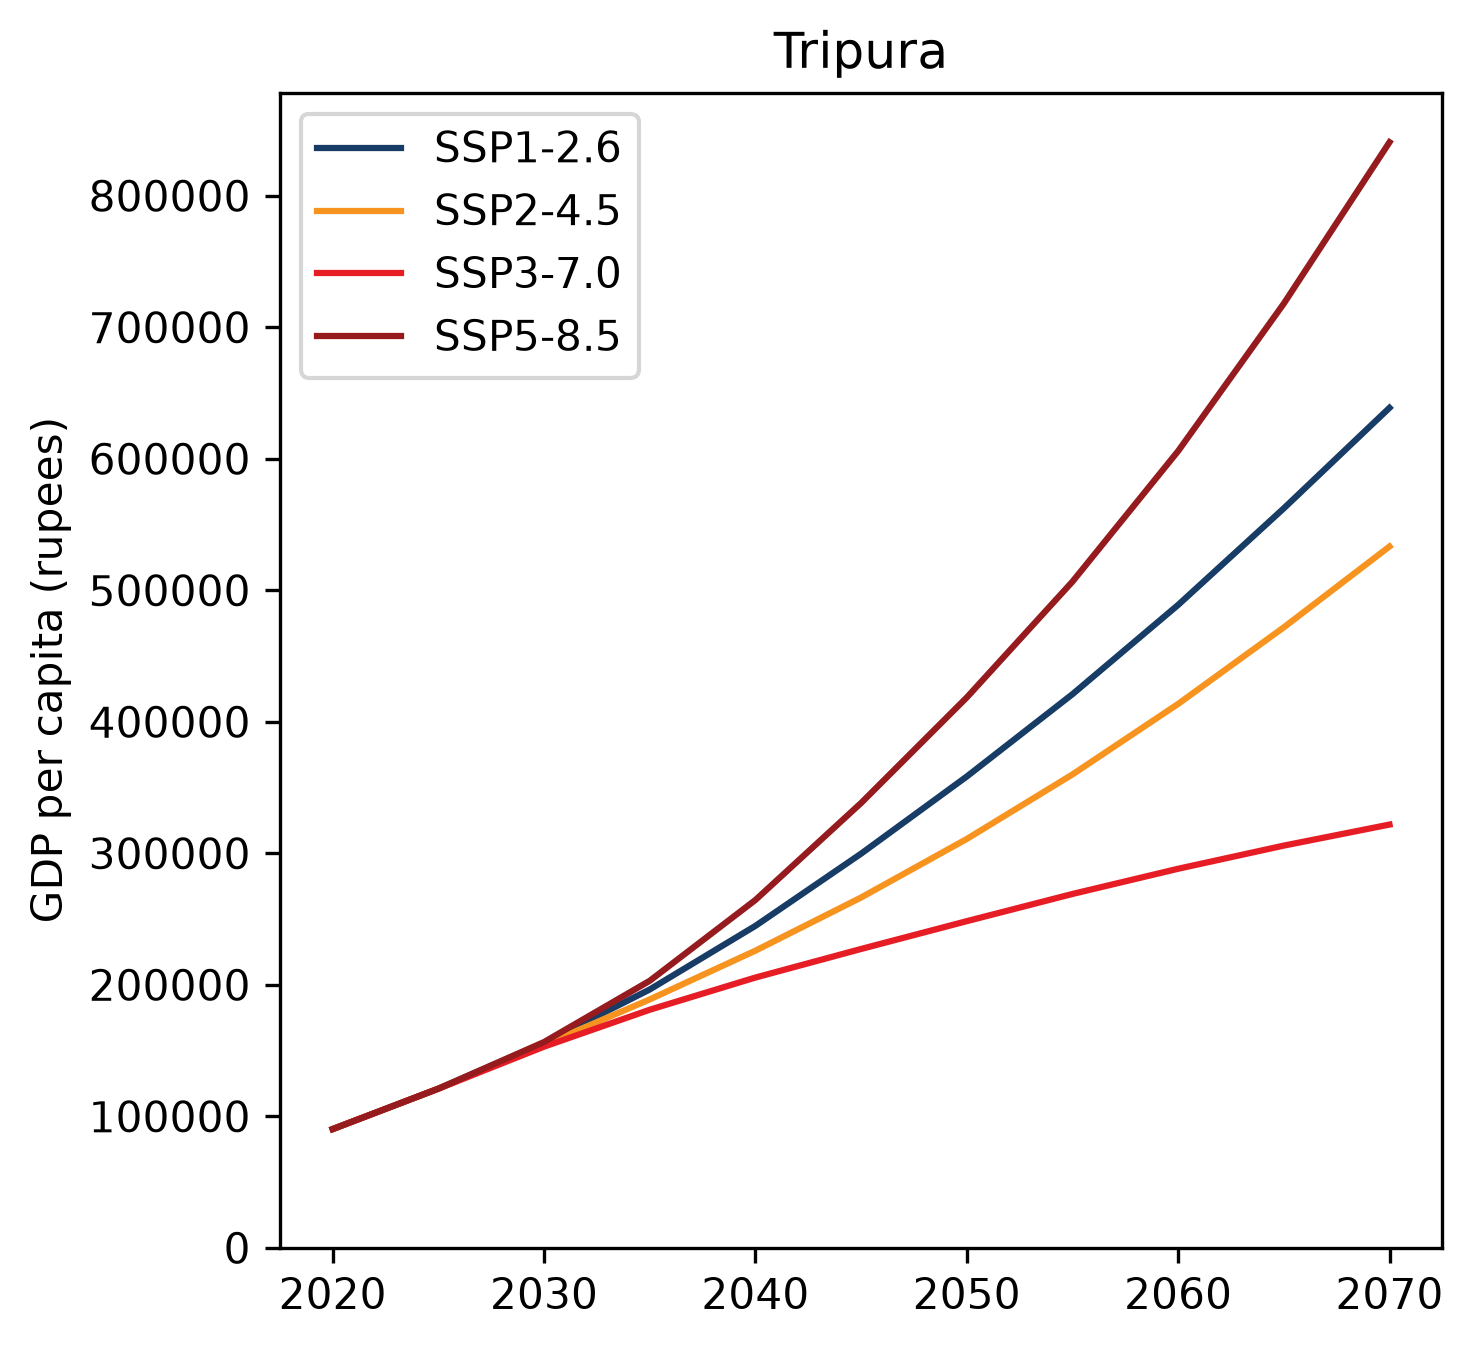
\includegraphics[height=0.25\textheight]{figures/projection_states/projection_gdp_per_capita_Tripura.png}\\
   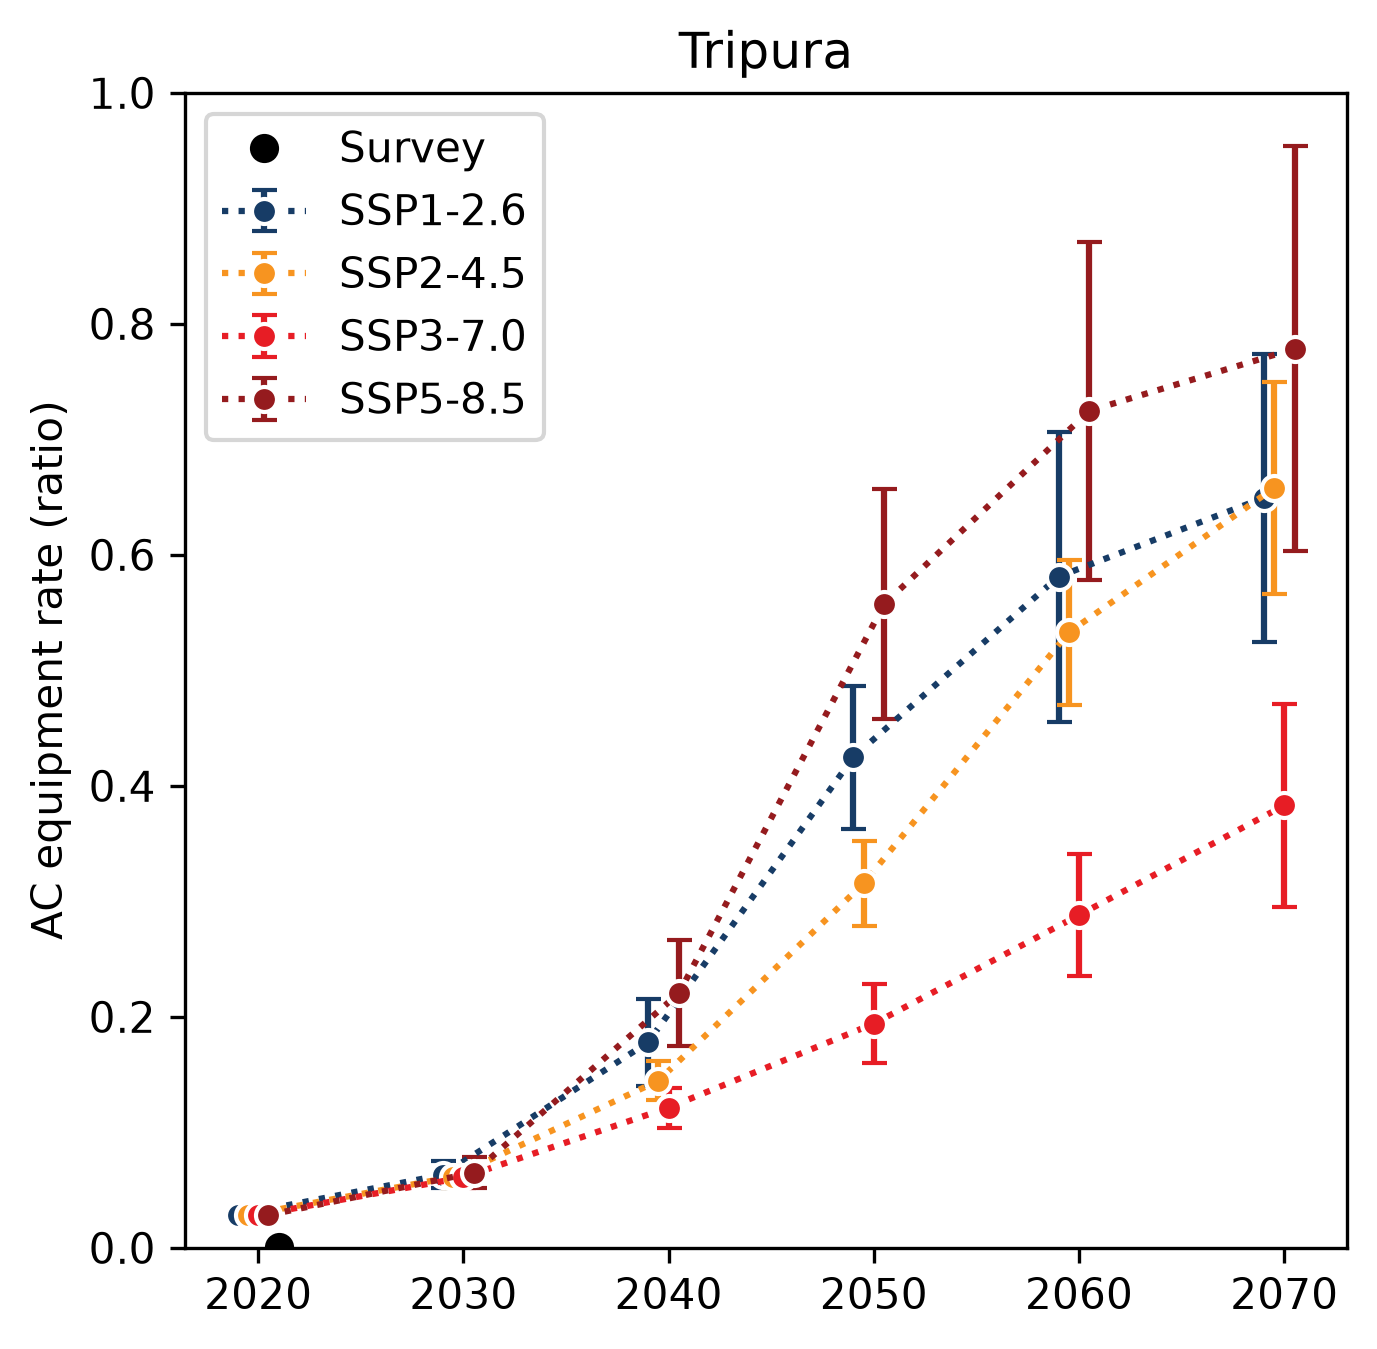
\includegraphics[height=0.25\textheight]{figures/projection_states/projection_ac_rate_Tripura.png}\hfill
   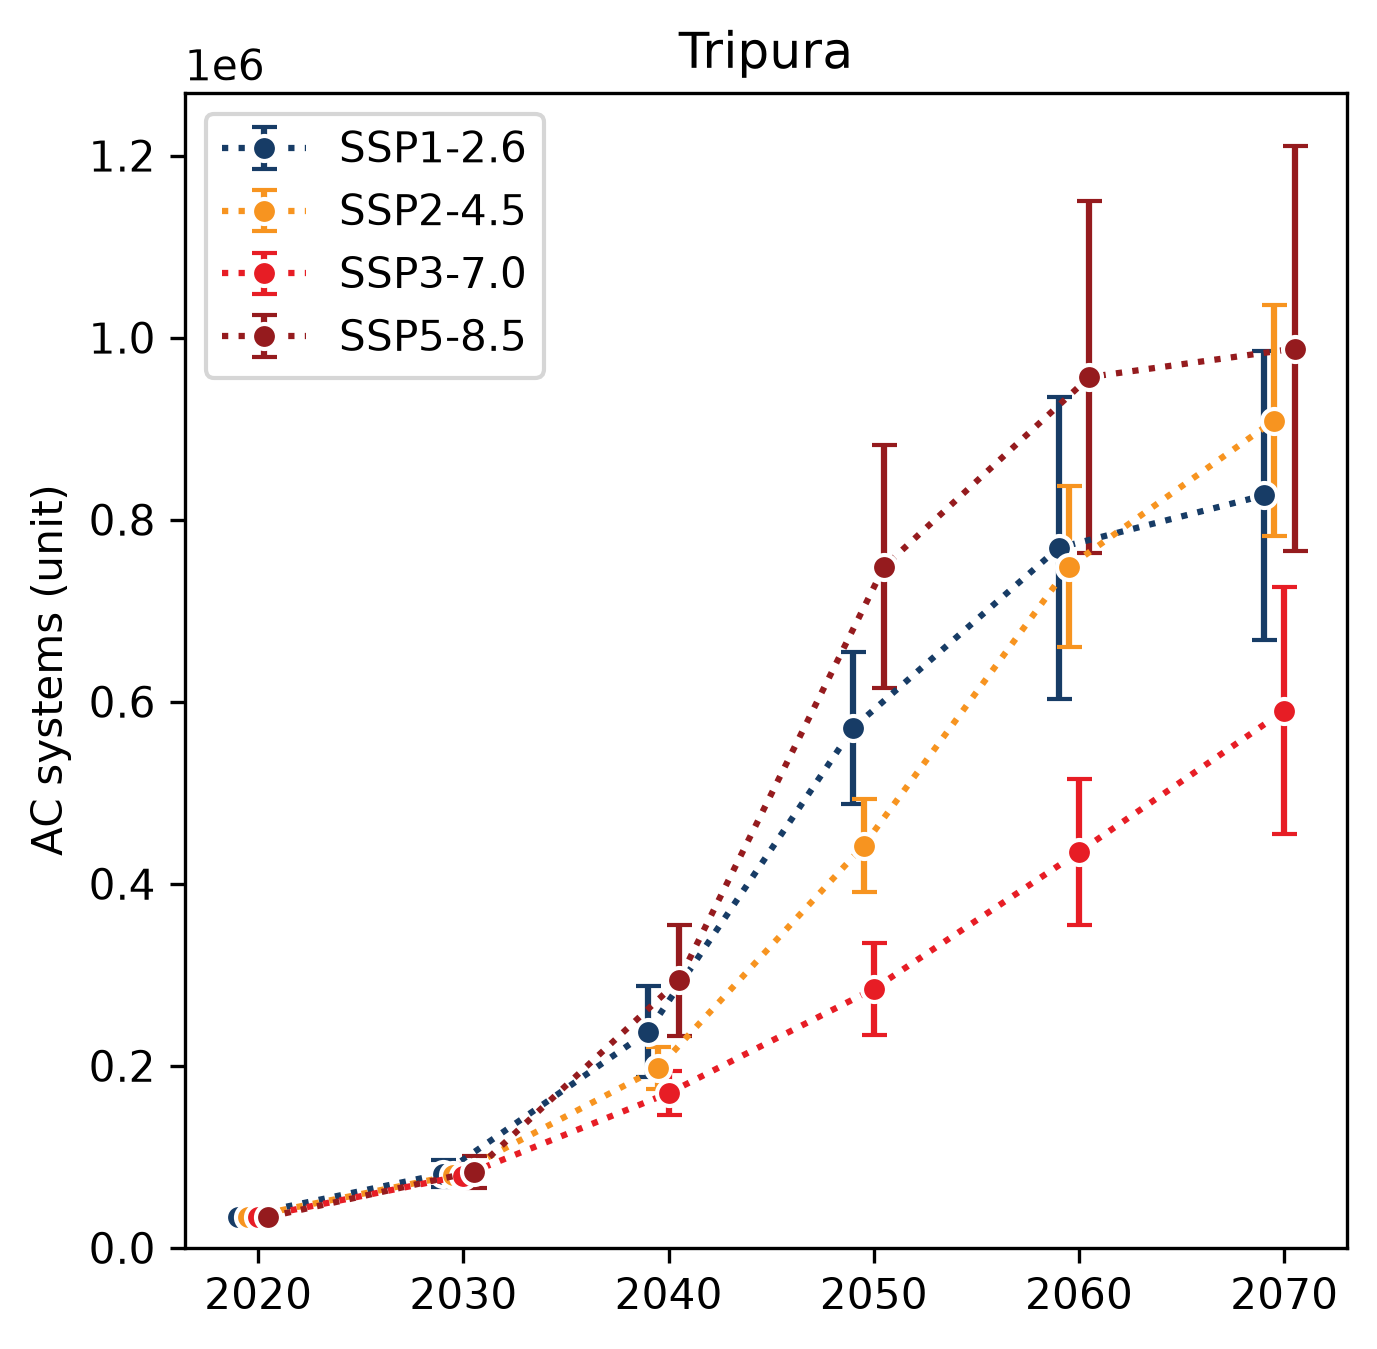
\includegraphics[height=0.25\textheight]{figures/projection_states/projection_ac_systems_Tripura.png}
   \caption{Projections des différentes variables pour Tripura}
\end{figure}

\clearpage

\subsubsection{Uttar Pradesh}

\begin{figure}[ht]
   \centering
   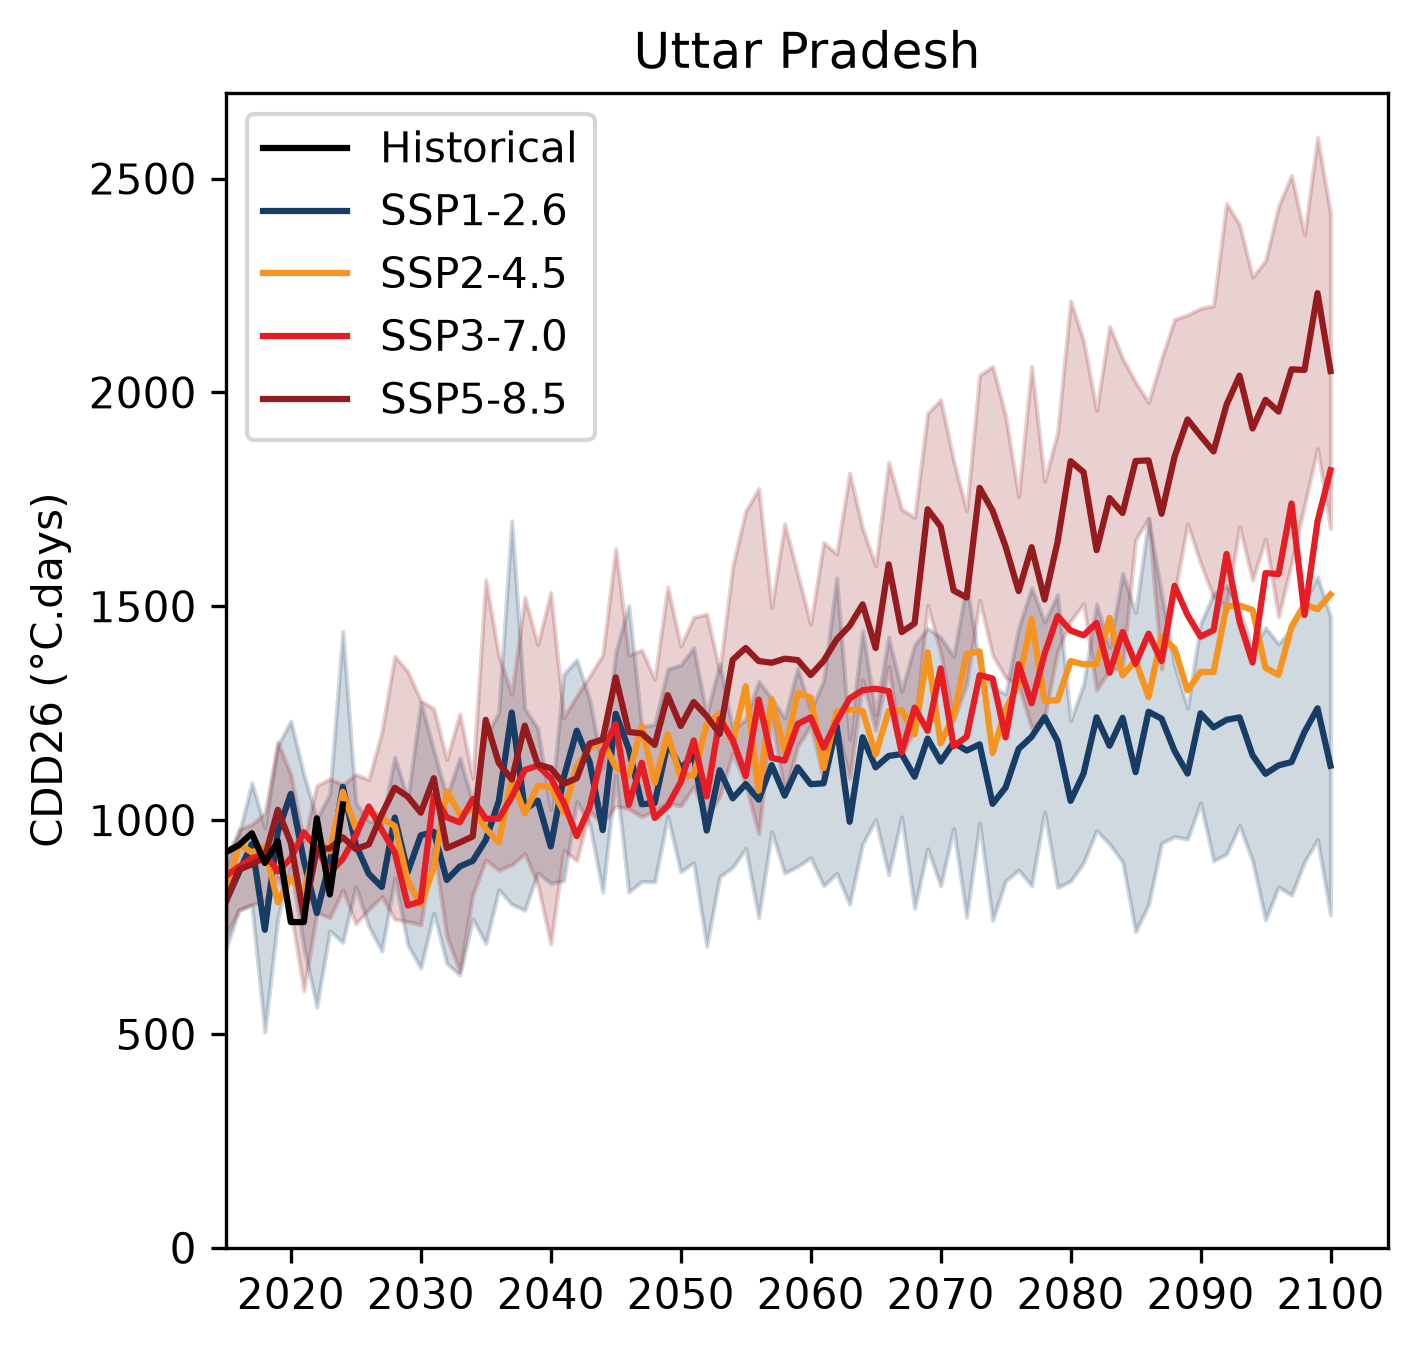
\includegraphics[height=0.25\textheight]{figures/projection_states/projection_cdd26_Uttar Pradesh.png}\hfill
   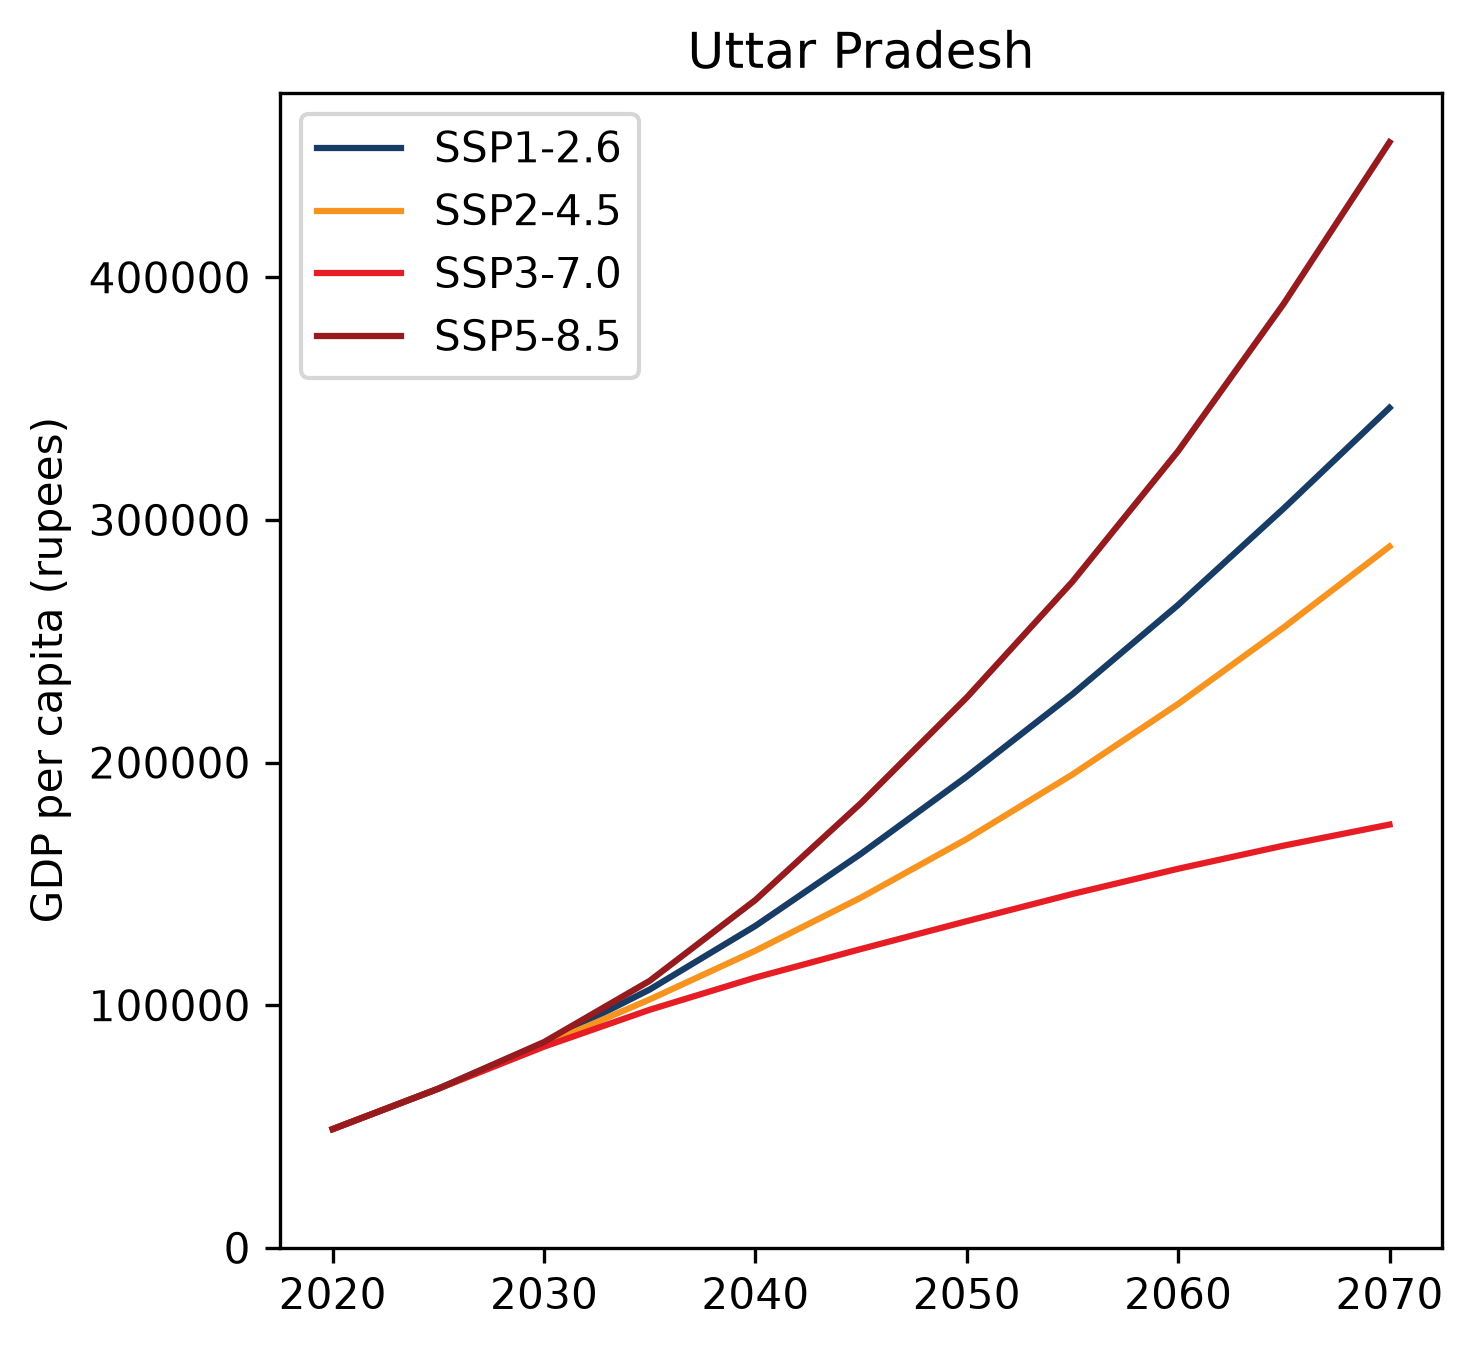
\includegraphics[height=0.25\textheight]{figures/projection_states/projection_gdp_per_capita_Uttar Pradesh.png}\\
   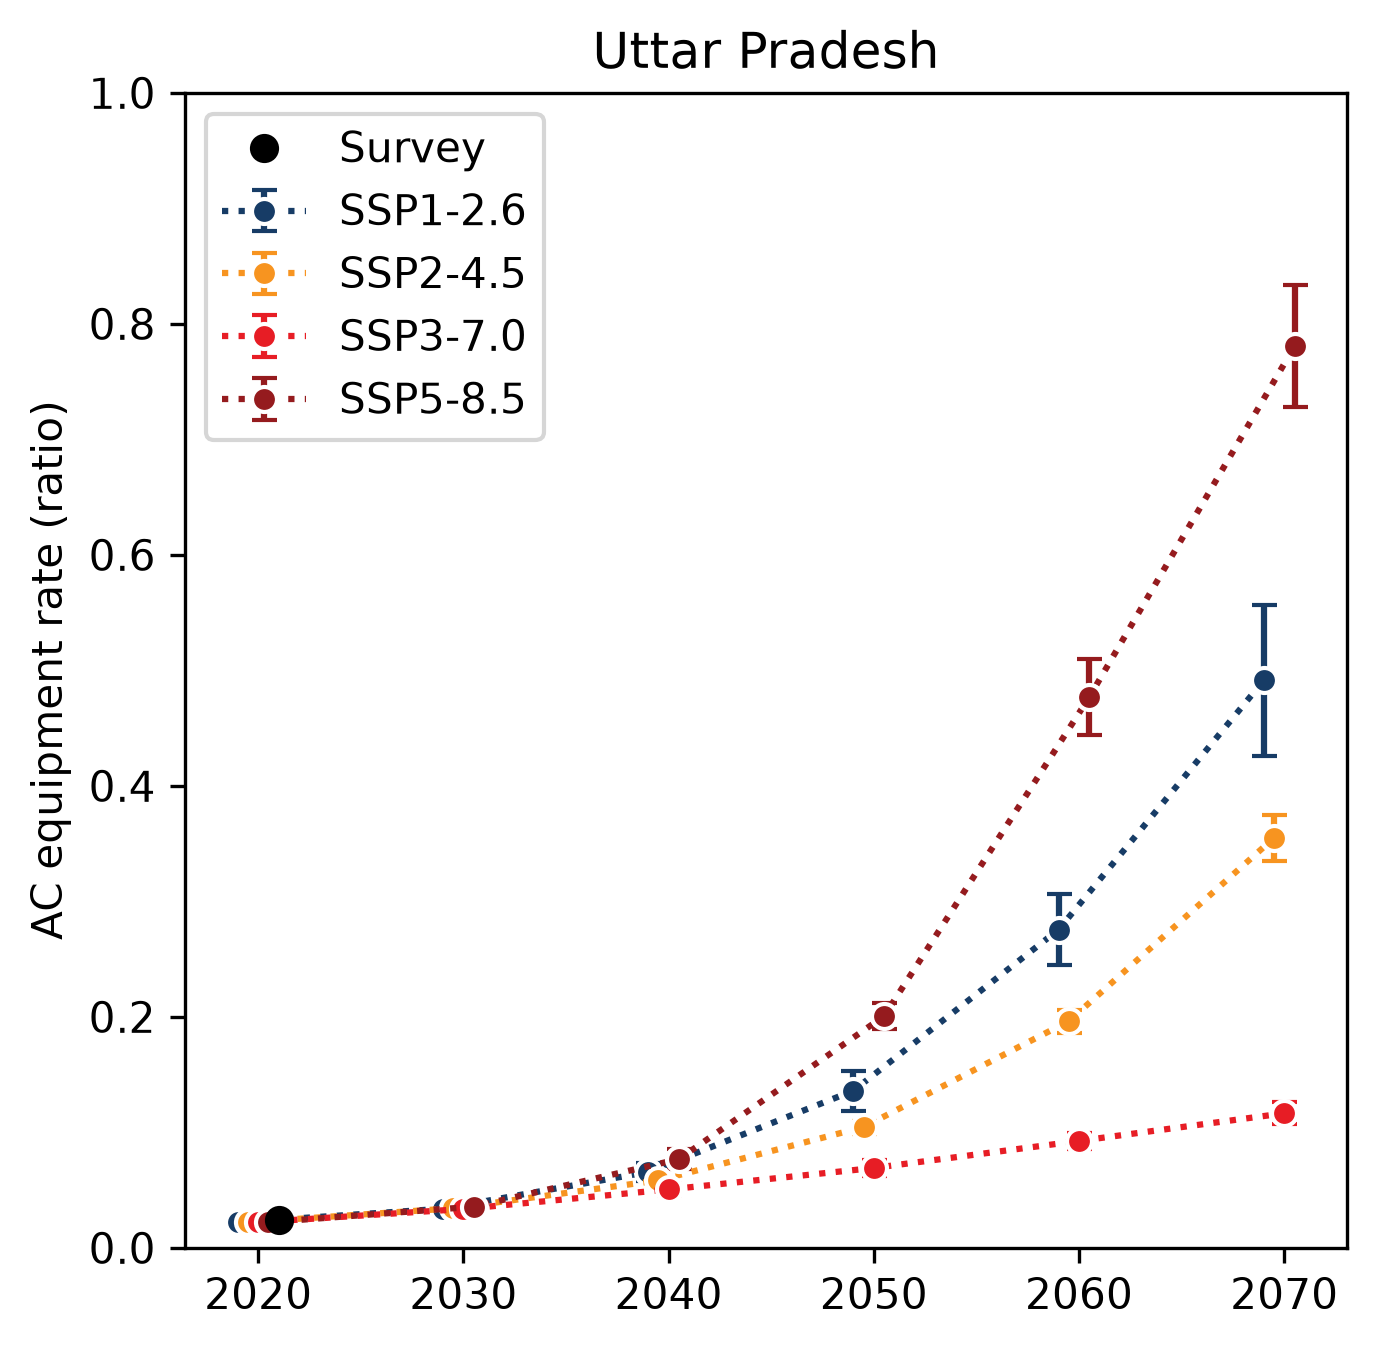
\includegraphics[height=0.25\textheight]{figures/projection_states/projection_ac_rate_Uttar Pradesh.png}\hfill
   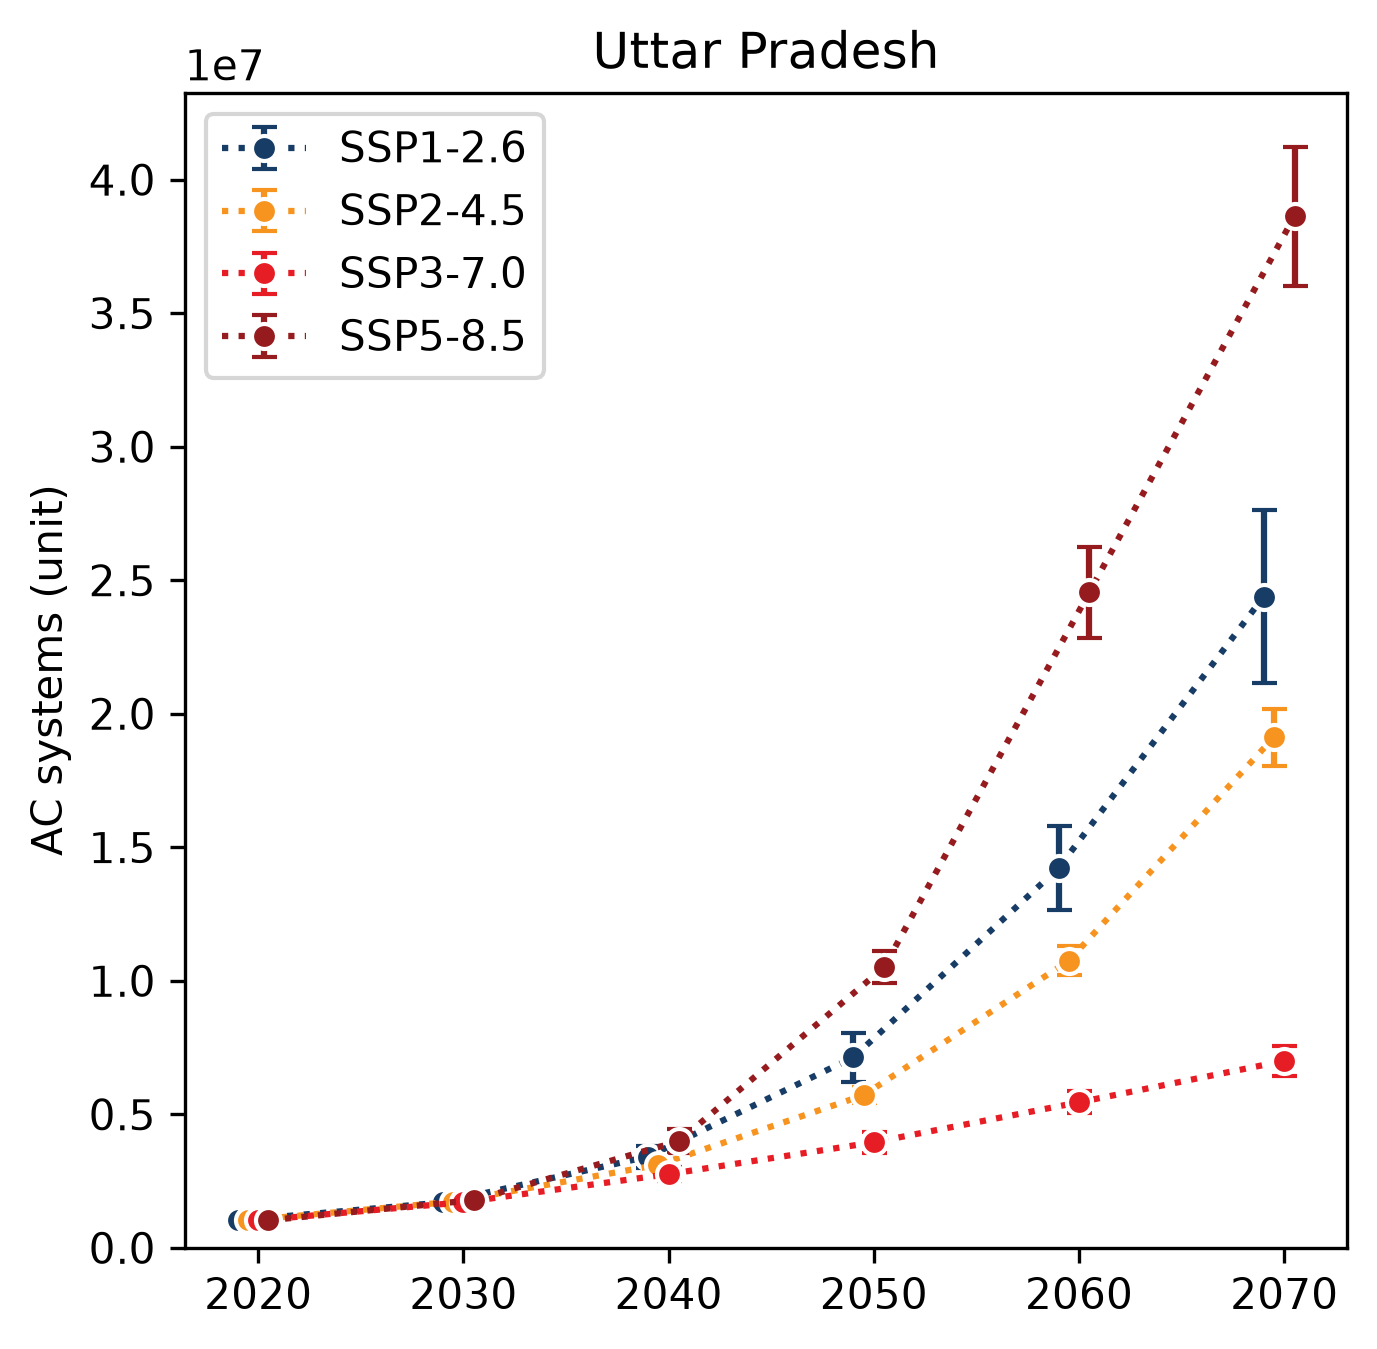
\includegraphics[height=0.25\textheight]{figures/projection_states/projection_ac_systems_Uttar Pradesh.png}
   \caption{Projections des différentes variables pour Uttar Pradesh}
\end{figure}

\clearpage

\subsubsection{Uttarakhand}

\begin{figure}[ht]
   \centering
   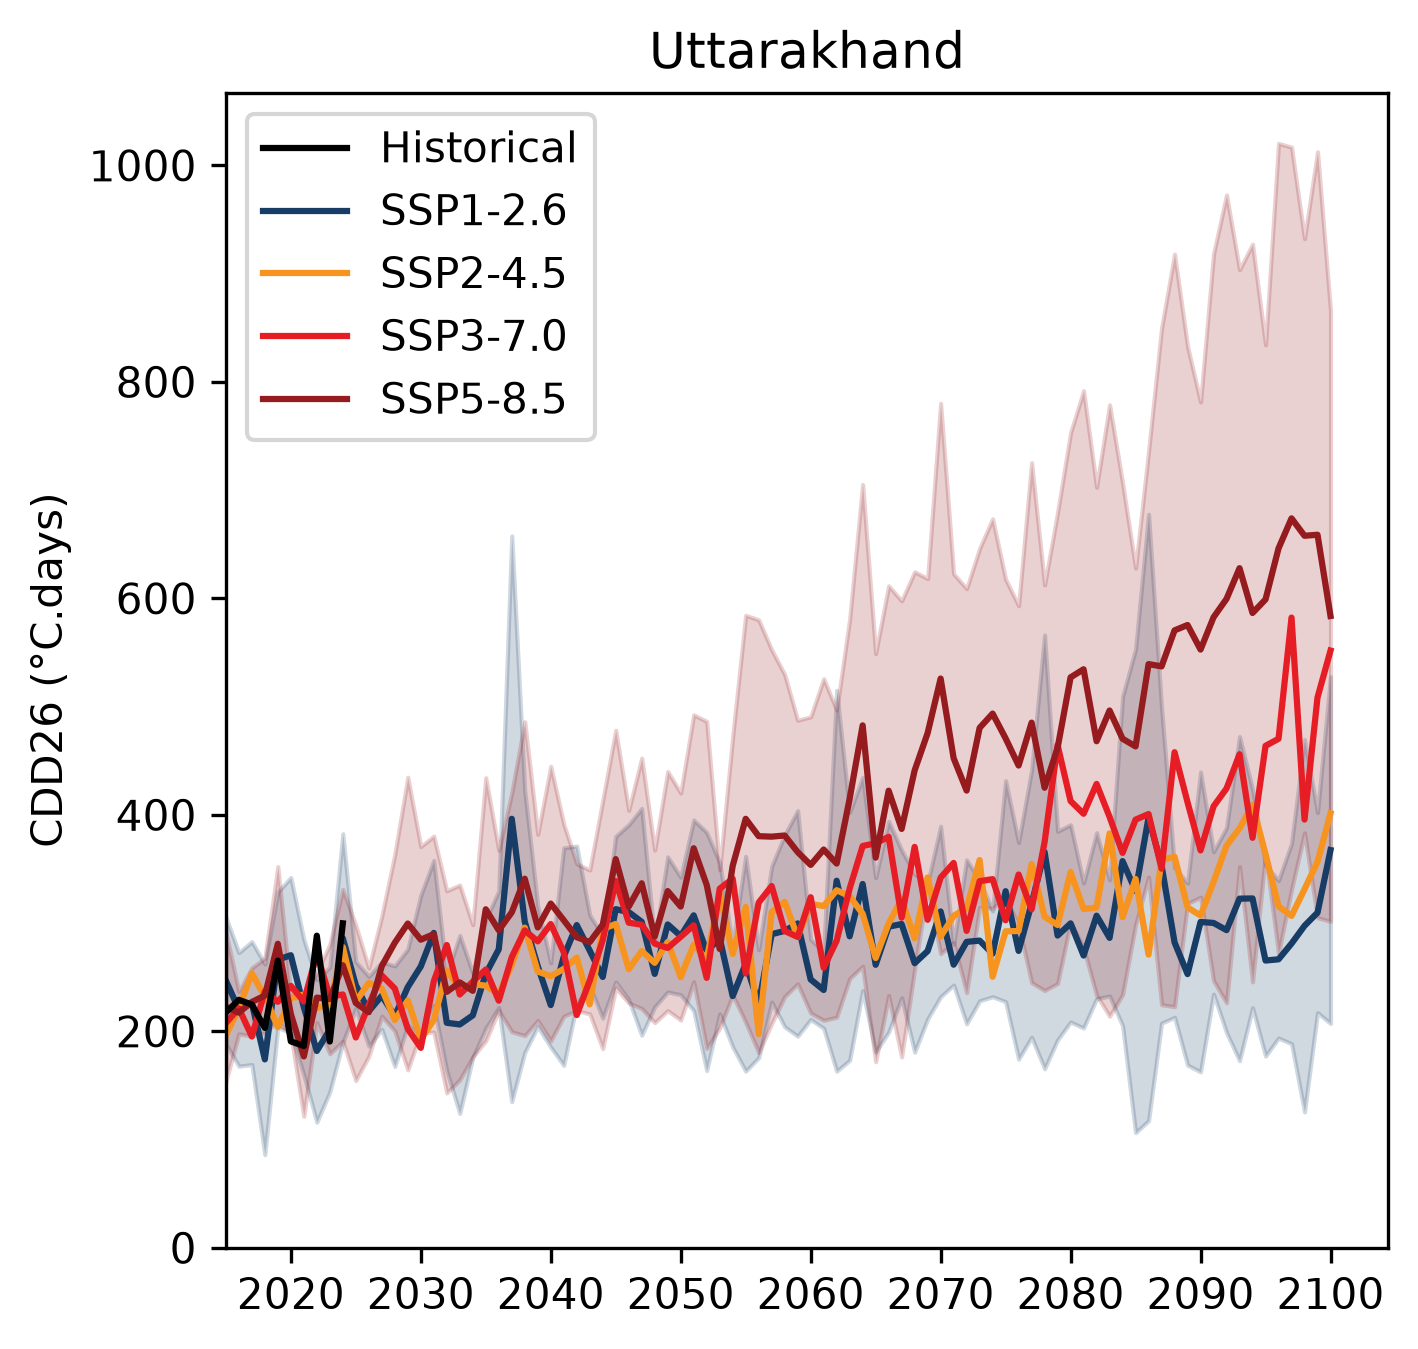
\includegraphics[height=0.25\textheight]{figures/projection_states/projection_cdd26_Uttarakhand.png}\hfill
   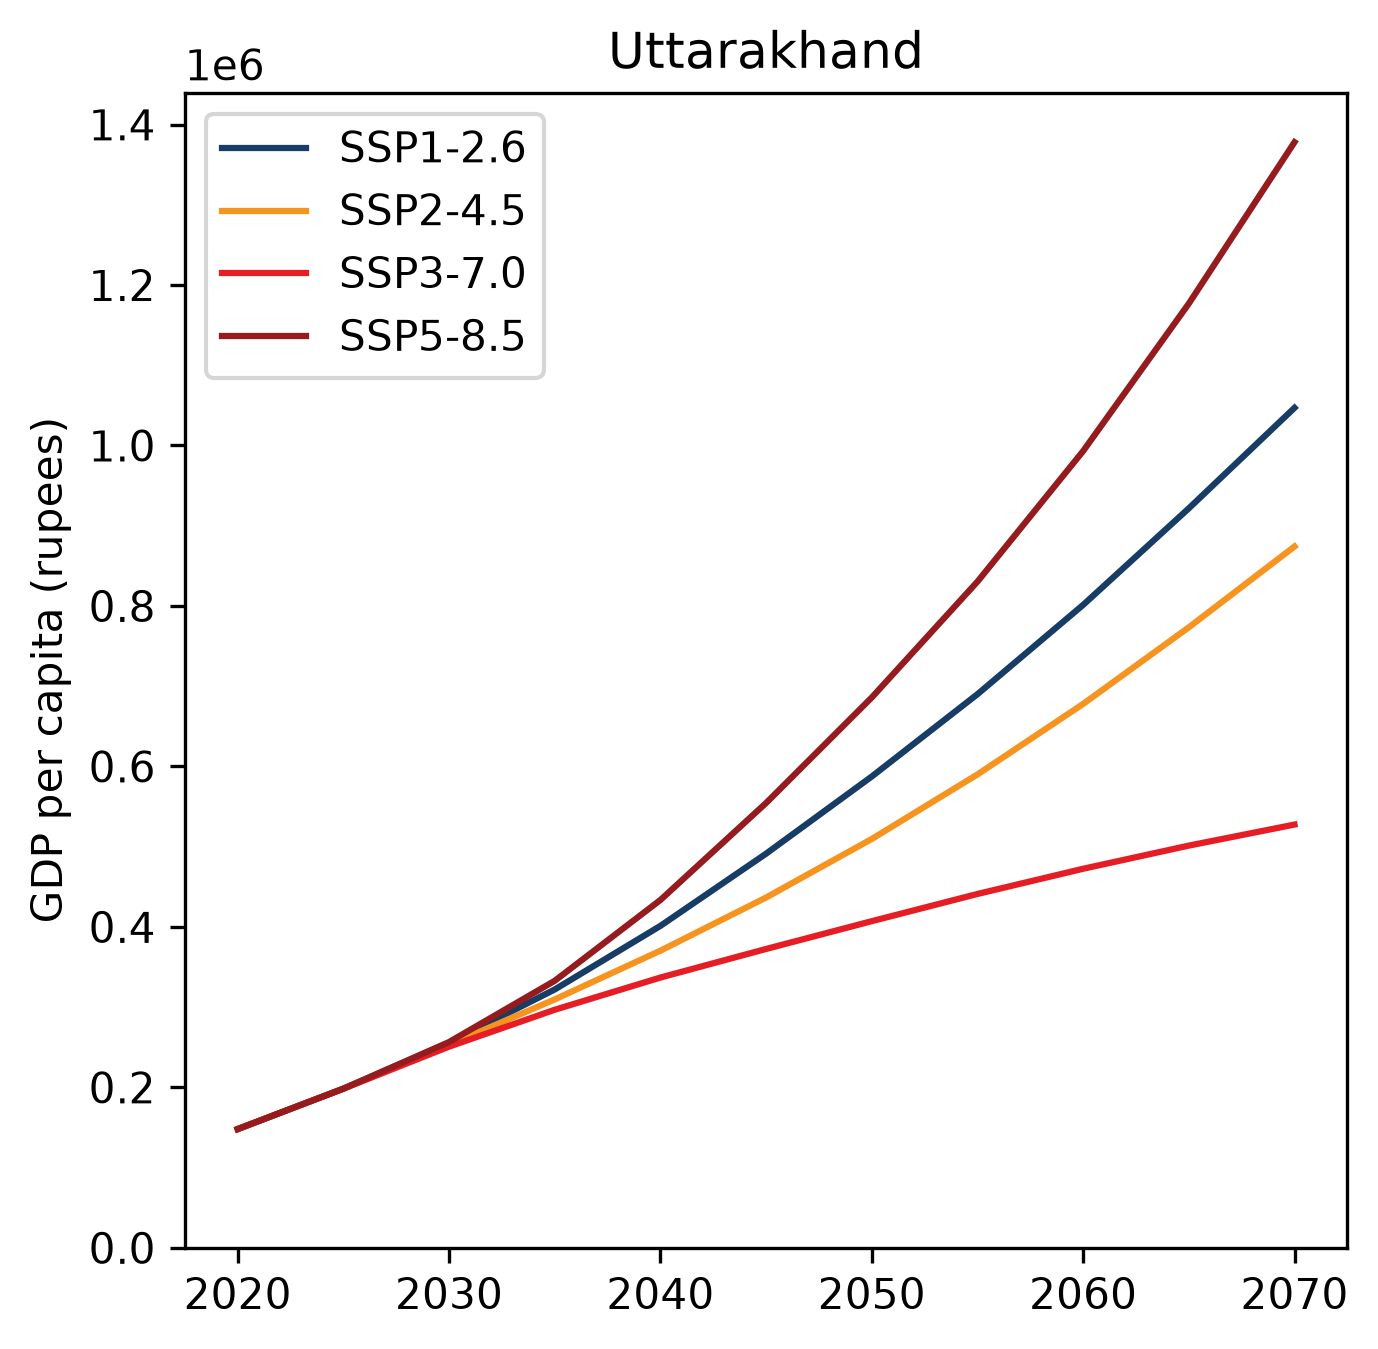
\includegraphics[height=0.25\textheight]{figures/projection_states/projection_gdp_per_capita_Uttarakhand.png}\\
   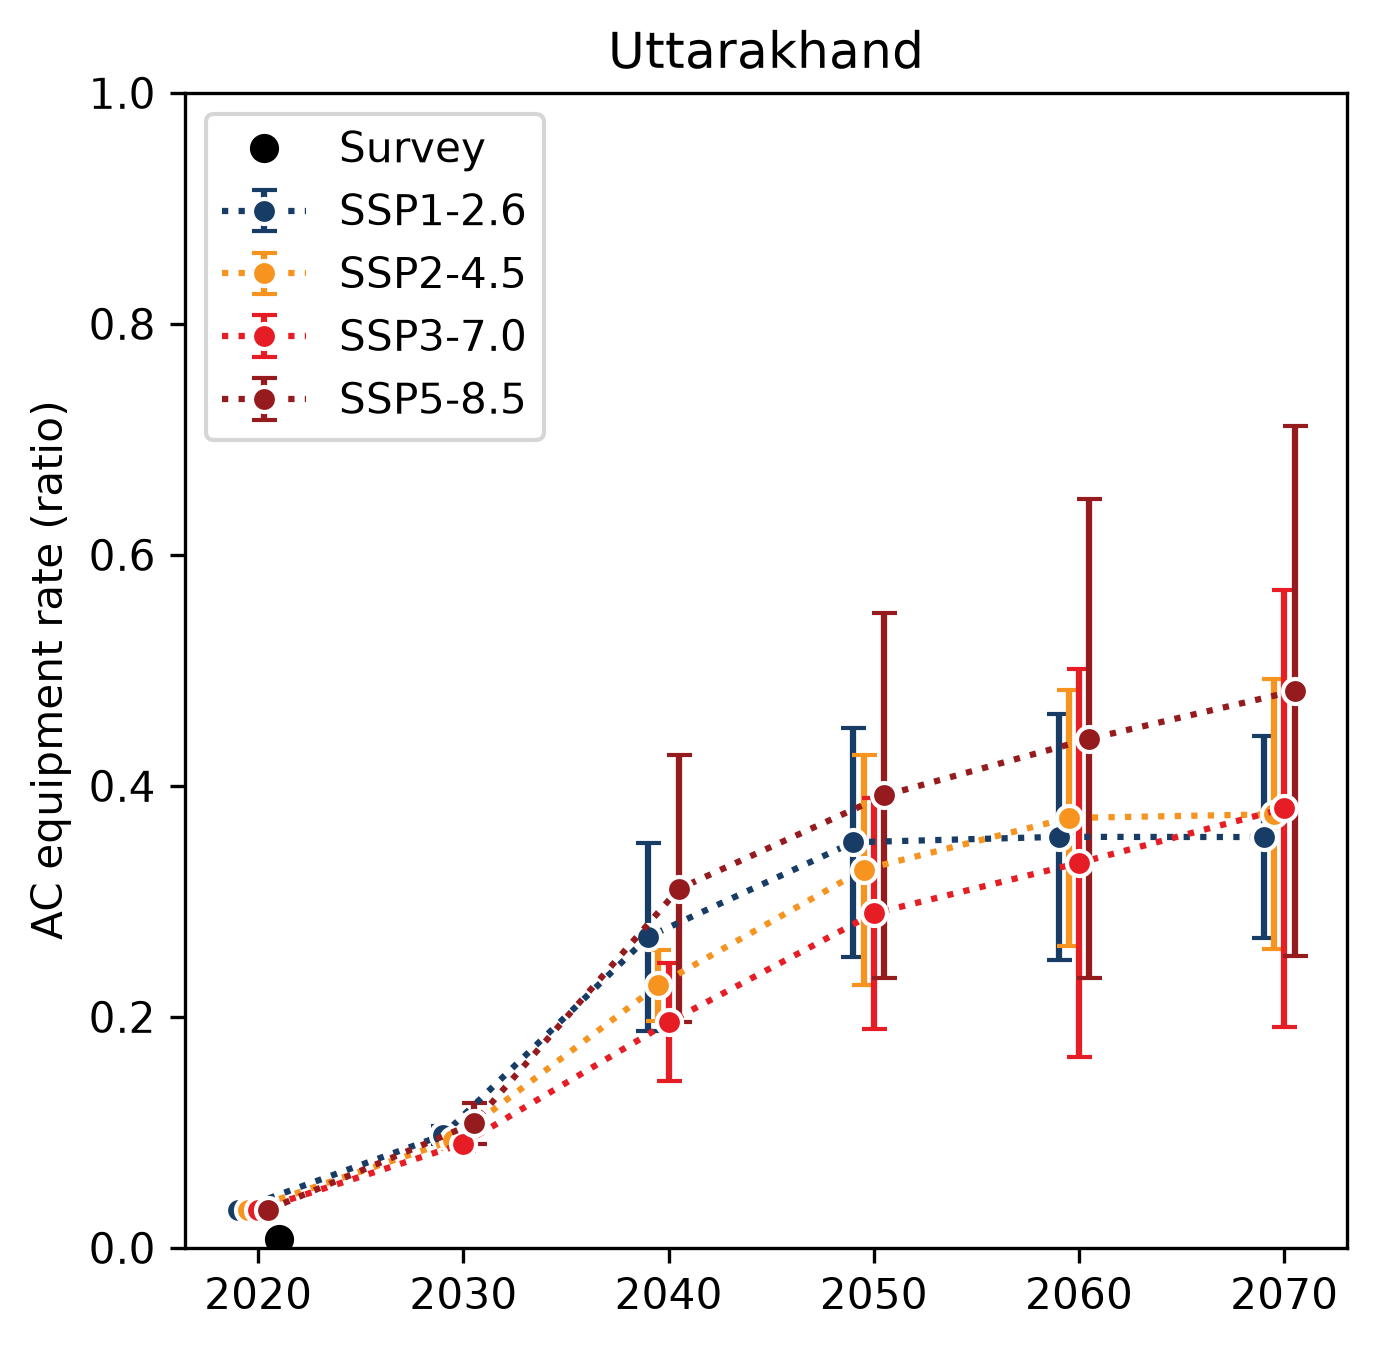
\includegraphics[height=0.25\textheight]{figures/projection_states/projection_ac_rate_Uttarakhand.png}\hfill
   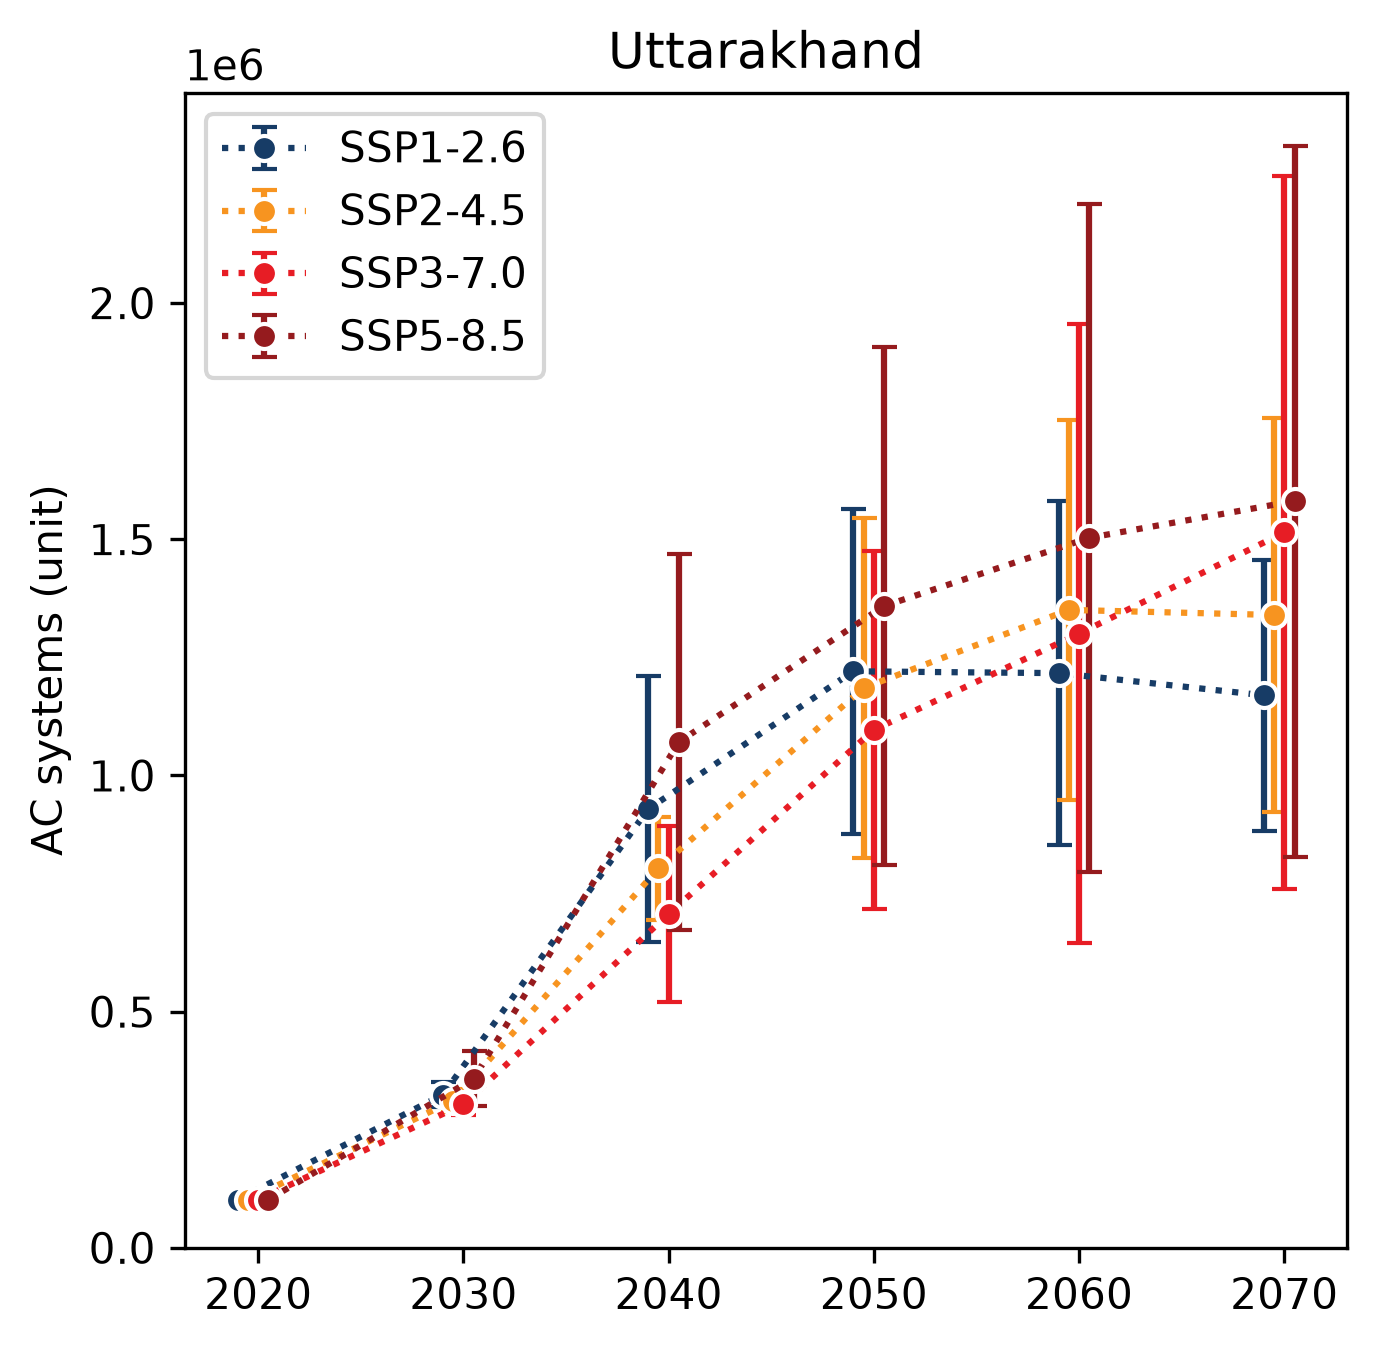
\includegraphics[height=0.25\textheight]{figures/projection_states/projection_ac_systems_Uttarakhand.png}
   \caption{Projections des différentes variables pour Uttarakhand}
\end{figure}

\clearpage

\subsubsection{West Bengal}

\begin{figure}[ht]
   \centering
   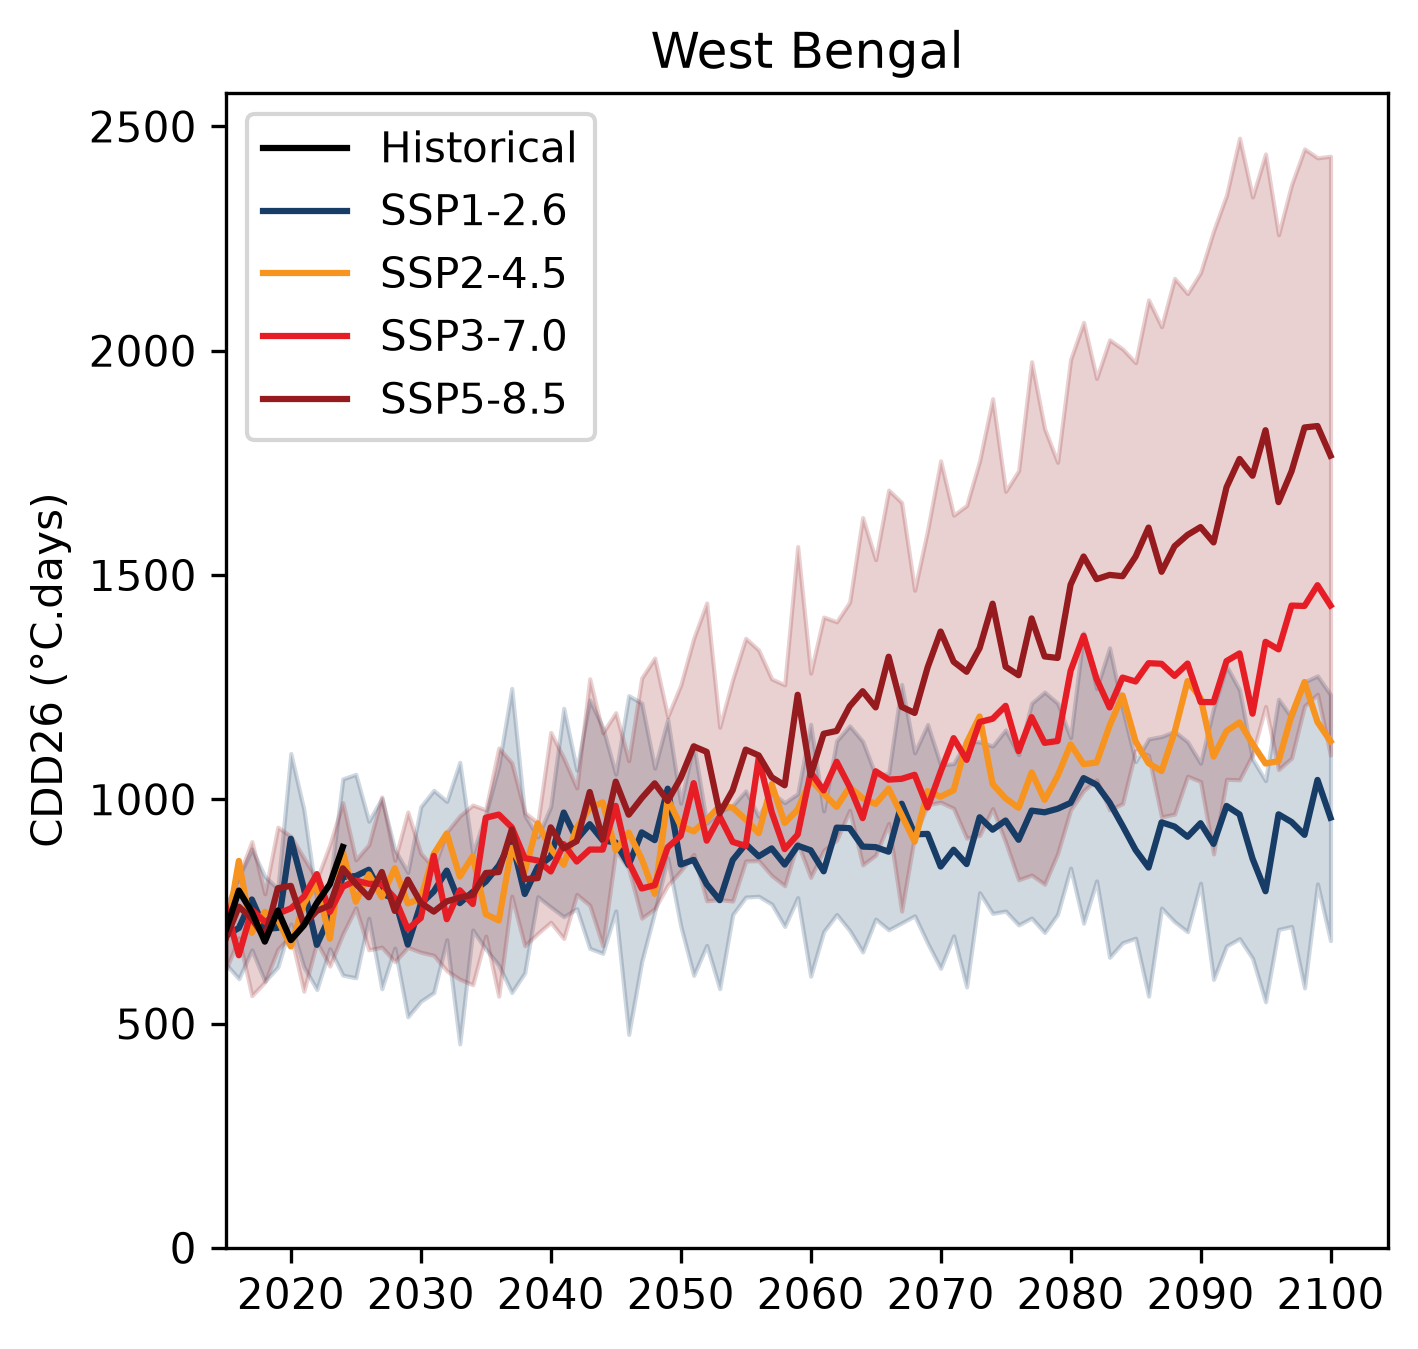
\includegraphics[height=0.25\textheight]{figures/projection_states/projection_cdd26_West Bengal.png}\hfill
   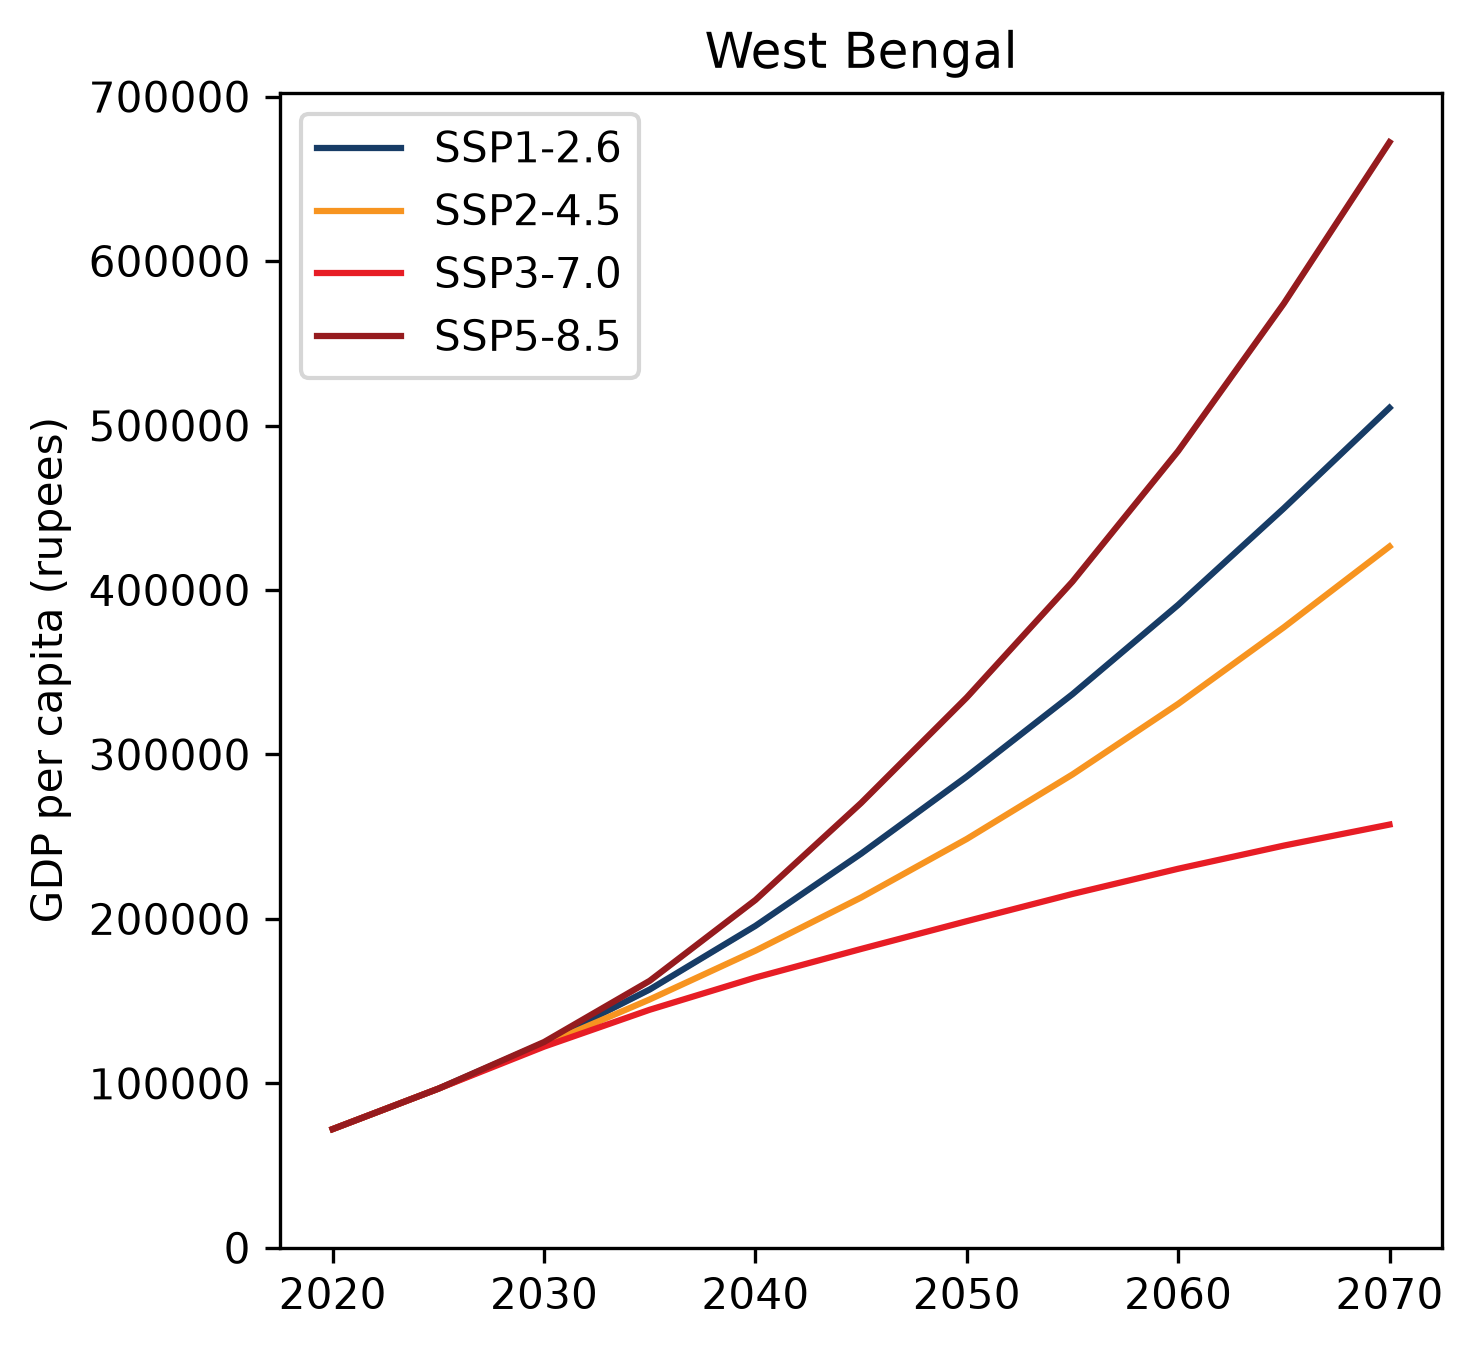
\includegraphics[height=0.25\textheight]{figures/projection_states/projection_gdp_per_capita_West Bengal.png}\\
   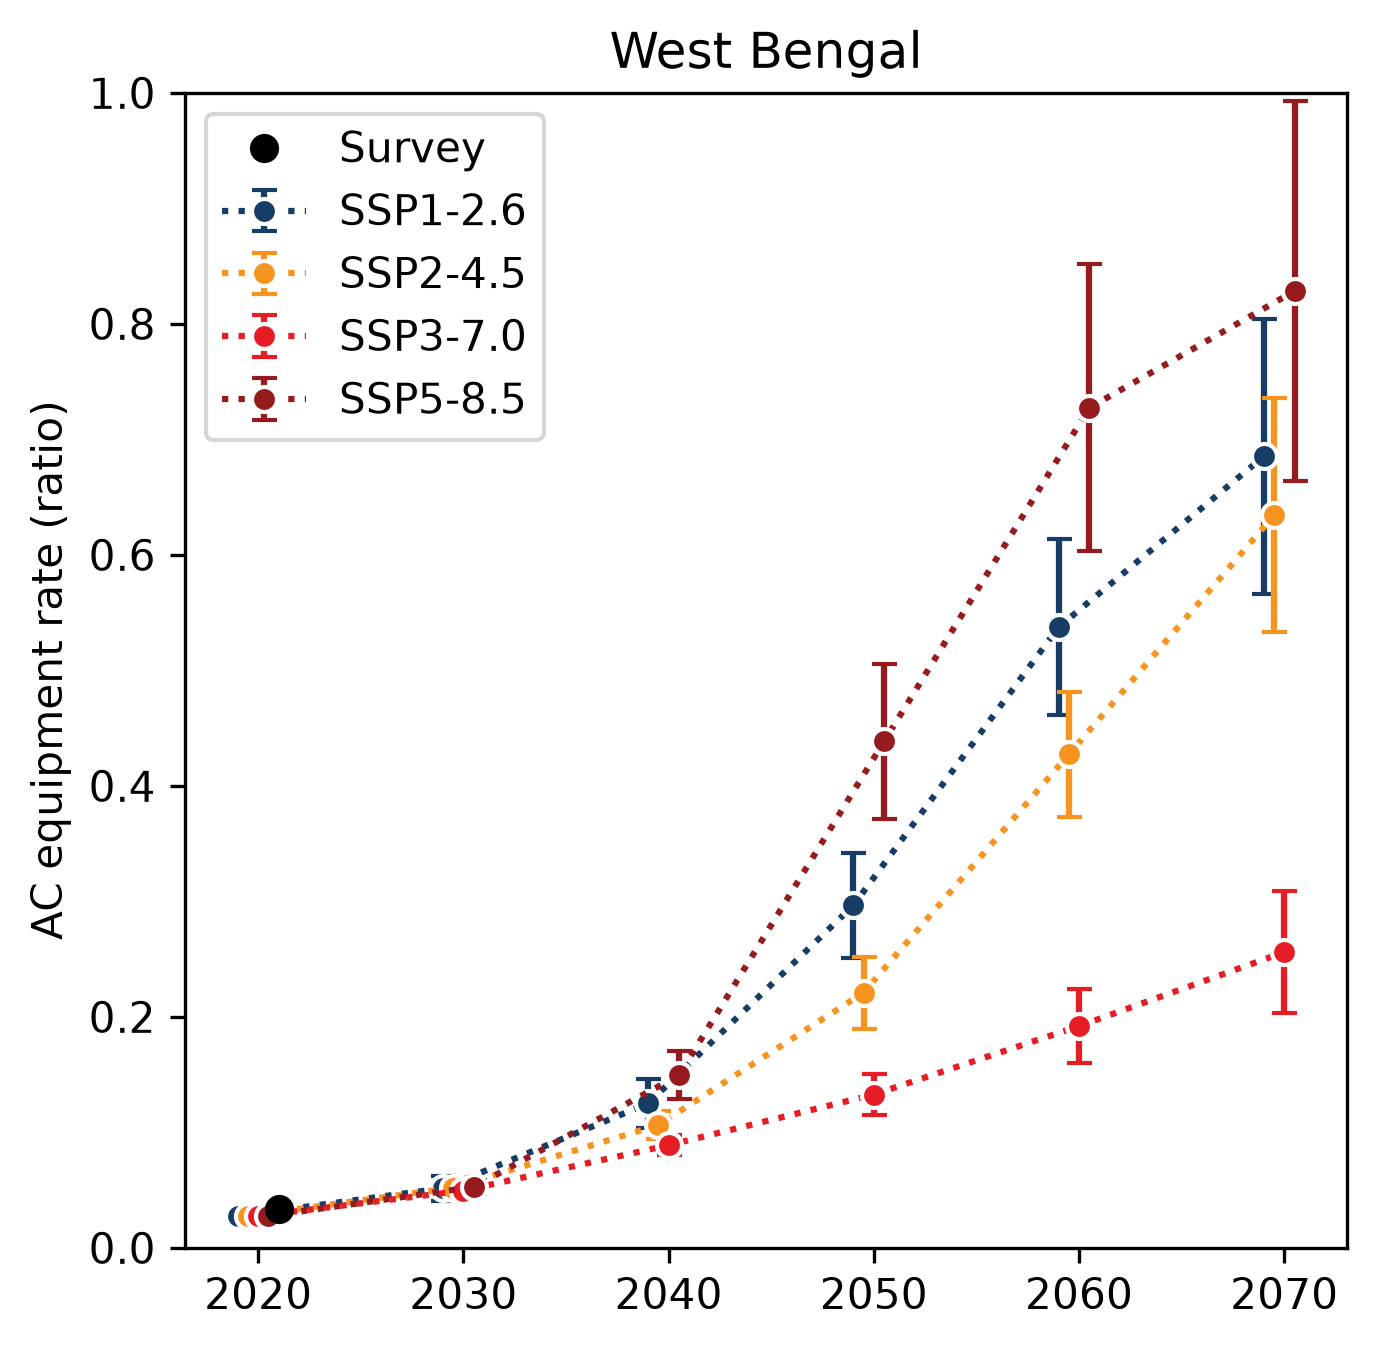
\includegraphics[height=0.25\textheight]{figures/projection_states/projection_ac_rate_West Bengal.png}\hfill
   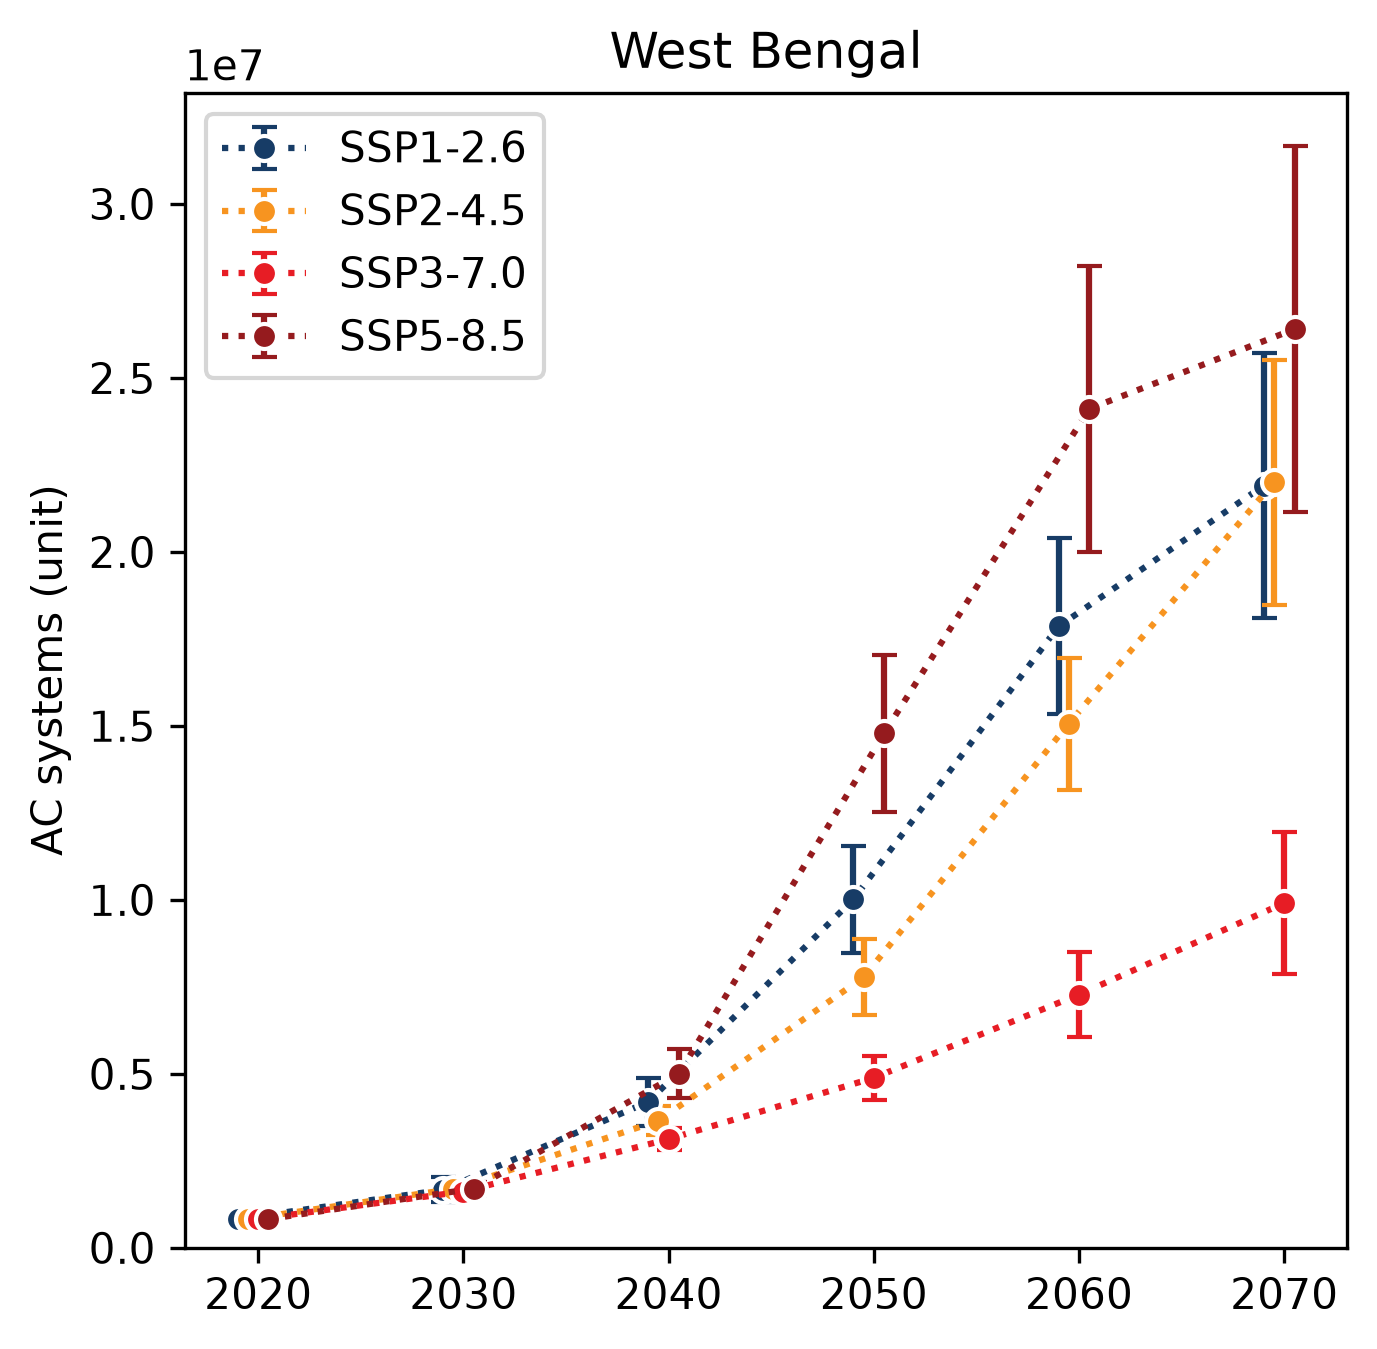
\includegraphics[height=0.25\textheight]{figures/projection_states/projection_ac_systems_West Bengal.png}
   \caption{Projections des différentes variables pour West Bengal}
\end{figure}



\clearpage
\printbibliography
\end{document}